%% Abstract.

\chapter*{Abstract}
\addcontentsline{toc}{chapter}{Abstract}

Galërkin methods have significantly influenced numerical analysis by providing a unified framework for approximating solutions to differential equations. Their versatility has led to advancements in stability, accuracy, and computational efficiency, with applications spanning fluid dynamics, electromagnetics, and high-order numerical simulations.

This thesis investigates the discontinuous Galërkin method for the space-time discretization of a particular class of PDEs.

After a brief review of the preliminaries, the method is first formally introduced for the broader class of parabolic problems and later specialized to the convection-diffusion-reaction problem, for which an explicit derivation and error analysis are carried out. It is shown that, under certain assumptions of mesh shape regularity and sufficient regularity of the exact solution, the errors are of order $\BigO{h^p + \tau^q}$, where $p$ and $q$ represent the orders of approximation in space and time, respectively.

The algorithm is implemented from scratch in \lstinline{C++23}, requiring the development of methods and classes for handling standard algebraic objects, a polygonal mesher, and a solver for sparse linear systems, as well as tailored methods for constructing the problem based on its discretization and performing the necessary quadratures.

Numerical tests performed using the aforementioned implementation in both the parabolic and hyperbolic cases validate the algorithm and its implementation, confirming the expected orders of convergence for the error derived in the theoretical analysis across various norms.

The results obtained not only confirm the effectiveness of this approach but also lay the groundwork for future research, particularly in the direction of adaptivity.

%% Table of Contents.

\newpage
\tableofcontents
\thispagestyle{plain}

%% Chapters.

% Introduction.

\newpage
\chapter*{Introduction}
\addcontentsline{toc}{chapter}{Introduction} \label{chapter:introduction}
\pagenumbering{arabic}

% \begin{epigraphs}
%     \qitem{TBA}{TBA}
% \end{epigraphs}

\section{Background and Motivation}

\acrfull{pdes} are fundamental in modeling a wide range of physical, biological, and engineering phenomena, including fluid dynamics, electromagnetism, and structural mechanics. Their study dates back to the works of Euler, Laplace, and Fourier, who formulated many of the classical equations still used today. Over time, the development of solution techniques has played a crucial role in advancing physics, engineering, and applied mathematics. However, solving \acrshort{pdes} analytically is often infeasible, except for specific cases with simple geometries and boundary conditions. This limitation necessitates numerical methods that approximate solutions efficiently and accurately.

Among numerical techniques, Galërkin methods have significantly influenced computational mathematics. First introduced by Boris Galërkin in the early 20th century, these methods provide a systematic framework for approximating \acrshort{pdes} solutions by projecting them onto a finite-dimensional function space. They have since evolved into various formulations, including the \acrfull{fem} and the \acrfull{dgm}, both of which offer significant advantages. By transforming the original problem into a system of algebraic equations, these methods enable numerical solutions to complex \acrshort{pdes} that arise in real-world applications. Their flexibility in handling irregular geometries, adaptive refinement, and stability properties makes them particularly effective for problems where classical approaches, such as finite difference methods, struggle.

\newpage
\section{Outline of the Thesis}

This thesis focuses on the discontinuous Galërkin method, first introduced in \citetitle{Reed1973} as an extension of Galërkin methods that allows discontinuities between elements, offering enhanced stability properties and adaptability for high-order approximations. The study is structured to provide a coherent progression from theoretical foundations to numerical implementation and results.

\Cref{chapter:preliminaries} provides a brief review of the necessary mathematical preliminaries, introducing key function spaces that are fundamental for formulating weak solutions of \acrshort{pdes}. This chapter establishes notation and ensures completeness, laying the groundwork for the subsequent theoretical developments.

\Cref{chapter:dg} investigates the \acrshort{dgm} for a class of parabolic problems. After a brief introduction to Bochner spaces, it presents the model parabolic problem and its weak formulation. The chapter then develops a discretization that is continuous in space and discontinuous in time, analyzing its stability and accuracy.

\Cref{chapter:cdr} specialises the \acrshort{dgm} to the case of \acrfull{cdr} problems, detailing a discontinuous discretization of both space and time and providing a comprehensive error analysis of the method on which numerical tests are based.

\Cref{chapter:implementation} details the practical aspects of implementing the algorithm based on the \acrshort{dgm} for \acrshort{cdr} problems. It discusses the various components of the computational framework, including the handling of mesh generation, numerical integration, and the solution of the resulting algebraic systems. This chapter bridges the theoretical aspects developed in earlier chapters with their computational realization.

\Cref{chapter:results} presents the numerical results obtained by testing the implemented algorithm on a known exact solution of a \acrshort{cdr} problem. The chapter describes the testing conditions, evaluates the observed numerical behavior against theoretical predictions, and analyzes the effectiveness of the method. These results validate the algorithm and provide insights into its performance, concluding the thesis.

% Preliminaries.

\newpage
\chapter{Preliminaries} \label{chapter:preliminaries}

This chapter develops the mathematical basics behind the theory of \acrlong{pdes} and of the \acrlong{dgm}.

\section{Function Spaces}

The function spaces introduced in this section provide an ideal setting for studying and characterizing solutions of \acrshort{pdes}.

\subsection{Lebesgue Spaces}

Following \cite[p. 89]{Brezis2010}, let $(\Omega, \SA, \mu)$ denote a measure space, where $\Omega \subseteq \Rd{d}$, $\SA$ is a $\sigma$-algebra on $\Omega$, and $\mu$ is a measure. Assume that $\Omega$ is $\sigma$-finite, that is there exist $\left\{ \Omega_n \right\}_{n \in \N} \subset \SA$ such that:
\begin{align}
    & \Omega = \bigcup_{n \in \N} \Omega_n, \\
    & \mu(\Omega_n) < +\infty \text{ for all } n \in \N.
\end{align}

\begin{definition}[$\Lp{1}(\Omega, \SA, \mu)$]
    \begin{gather}
        \Lp{1}(\Omega, \SA, \mu) = \left\{ f \colon \Omega \rightarrow \R \text{ measurable such that } \int_{\Omega} \lvert f(\Vector{x}) \rvert ~ d \mu < \infty \right\},
    \end{gather}
    with:
    \begin{gather}
    \lVert f \rVert_{\Lp{1}(\Omega)} = \lVert f \rVert_{1} = \int_{\Omega} \lvert f(\Vector{x}) \rvert d \mu.
    \end{gather}
\end{definition}

Without losing generality, let $\Lp{1}(\Omega) = \Lp{1}(\Omega, \SA, \mu)$ in what follows.

\subsubsection{Known Results}

\begin{theorem}[Beppo Levi, or monotone convergence]
    Let $\left\{ f_n \right\}_{n \in \N} \subset \Lp{1}(\Omega)$ such that:
    \begin{align}
        & 0 \leq f_1(\Vector{x}) \leq \dots \leq f_n(\Vector{x}) \leq \dots < +\infty \text{ for } \mu \text{-a.e. } \Vector{x} \in \Omega, \\
        & \sup_{n \in \N} \int_\Omega f_n(\Vector{x}) ~ d \mu < +\infty,
    \end{align}
    then there exists $f \in \Lp{1}(\Omega)$ such that for $\mu$-a.e. $\Vector{x} \in \Omega$:
    \begin{gather}
        \lim_{n \rightarrow \infty} f_n(\Vector{x}) = f(\Vector{x}),
    \end{gather}
    and
    \begin{gather}
        \lim_{n \rightarrow \infty} \lVert f_n - f \rVert_1 = 0.
    \end{gather}
\end{theorem}

\begin{theorem}[Lebesgue, or dominated convergence]
    Let $\left\{ f_n \right\}_{n \in \N} \subset \Lp{1}(\Omega)$ for which there exists $g \in \Lp{1}(\Omega)$ such that for $\mu$-a.e. $\Vector{x} \in \Omega$:
    \begin{align}
        & \lim_{n \rightarrow \infty} f_n(\Vector{x}) = f(\Vector{x}), \\
        & \lvert f_n(\Vector{x}) \rvert < g(\Vector{x}),
    \end{align}
    then $f \in \Lp{1}(\Omega)$ and:
    \begin{gather}
        \lim_{n \rightarrow \infty} \lVert f_n - f \rVert_1 = 0.
    \end{gather}
\end{theorem}

\begin{lemma}[Fatou]
    Let $\left\{ f_n \right\}_{n \in \N} \subset \Lp{1}(\Omega)$ such that:
    \begin{align}
        & f_n(x) \geq 0 \text{ for } \mu \text{-a.e. } \Vector{x} \in \Omega, \\
        & \sup_{n \in \N} \int_{\Omega} f_n(\Vector{x}) ~ d \mu < +\infty,
    \end{align}
    then:
    \begin{gather}
        \int_{\Omega} \liminf_{n \rightarrow \infty} f_n(\Vector{x}) \leq \liminf_{n \rightarrow \infty} \int_{\Omega} f_n(\Vector{x}).
    \end{gather}
\end{lemma}

\subsubsection{Definition and Elementary Properties}

\begin{definition}[$\Lp{p}(\Omega)$]
    Let $1 < p < +\infty$,
    \begin{gather}
        \Lp{p}(\Omega) = \left\{ f \colon \Omega \rightarrow \R \text{ such that } \left| f \right|^p \in \Lp{1}(\Omega) \right\},
    \end{gather}
    with:
    \begin{gather}
    \lVert f \rVert_{\Lp{p}(\Omega)} = \lVert f \rVert_{p} = \left( \int_{\Omega} \lvert f(\Vector{x}) \rvert^p ~ d \mu \right)^{1/p}.
    \end{gather}
\end{definition}

\begin{definition}[$\Lp{\infty}(\Omega)$]
    Let $C \geq 0$,
    \begin{gather}
        \Lp{\infty}(\Omega) = \left\{ f \colon \Omega \rightarrow \R \text{ measurable such that } \lvert f(\Vector{x}) \rvert < C \text{ for } \mu \text{-a.e. } \Vector{x} \in \Omega \right\},
    \end{gather}
    with:
    \begin{gather}
    \lVert f \rVert_{\Lp{\infty}(\Omega)} = \lVert f \rVert_{\infty} = \inf_{C \geq 0} \left\{ \lvert f(\Vector{x}) \rvert < C \text{ for } \mu \text{-a.e. } \Vector{x} \in \Omega \right\}.
    \end{gather}
\end{definition}

\begin{theorem}
    Let $1 \leq p \leq +\infty$, then $\Lp{p}(\Omega)$ is a vector space and $\lVert \cdot \rVert_p$ is a norm.
\end{theorem}

\begin{theorem}[Fischer-Riesz]
    Let $1 \leq p \leq +\infty$, then $(\Lp{p}(\Omega), \lVert \cdot \rVert_p)$ is a Banach space.
\end{theorem}

\begin{definition}[Conjugate exponent]
    Let $1 \leq p \leq +\infty$, denote by $p^{\prime}$ its conjugate exponent defined by:
    \begin{gather}
        \frac{1}{p} + \frac{1}{p^{\prime}} = 1.
    \end{gather}
\end{definition}

\begin{theorem}[Hölder's inequality]
    Let $1 \leq p \leq +\infty$, $f \in \Lp{p}(\Omega)$, and $g \in \Lp{p^{\prime}}(\Omega)$, then $fg \in \Lp{1}(\Omega)$ and:
    \begin{gather}
        \lVert fg \rVert_1 \leq \lVert f \rVert_p \lVert g \rVert_{p^{\prime}}.
    \end{gather}
\end{theorem}

\subsubsection{Characterizations}

\begin{theorem}
    Let $1 < p < +\infty$, then $\Lp{p}(\Omega)$ is reflexive.
\end{theorem}

\begin{theorem}[Riesz representation theorem for $1 < p < +\infty$] \label{theorem:riesz_p}
    Let $1 < p < +\infty$ and $\phi \in (\Lp{p}(\Omega))^*$, then for all $f \in \Lp{p}(\Omega)$ there exists a unique $u \in \Lp{p^{\prime}}(\Omega)$ such that:
    \begin{gather}
        \langle f, \phi \rangle = \int_{\Omega} f(\Vector{x}) u(\Vector{x}) ~ d \mu,
    \end{gather}
    and:
    \begin{gather}
        \lVert u \rVert_{p^{\prime}} = \lVert \phi \rVert_{p^{*}},
    \end{gather}
    where:
    \begin{gather}
        \lVert \phi \rVert_{p^{*}} = \lVert \phi \rVert_{(\Lp{p})^*}.
    \end{gather}
\end{theorem}

As a consequence of \autoref{theorem:riesz_p}, the following identification result can be stated:

\begin{theorem}
    Let $1 < p < +\infty$, then:
    \begin{gather}
        (\Lp{p}(\Omega))^* = \Lp{p^{\prime}}(\Omega).
    \end{gather}
\end{theorem}

\begin{theorem}[Riesz representation theorem for $p = 1$] \label{theorem:riesz_1}
    Let $\phi \in (\Lp{1}(\Omega))^*$, then for all $f \in \Lp{1}(\Omega)$ there exists a unique $u \in \Lp{\infty}(\Omega)$ such that:
    \begin{gather}
        \langle f, \phi \rangle = \int_{\Omega} f(\Vector{x}) u(\Vector{x}) ~ d \mu,
    \end{gather}
    and:
    \begin{gather}
        \lVert u \rVert_{\infty} = \lVert \phi \rVert_{1^{*}}.
    \end{gather}
\end{theorem}

As a consequence of \autoref{theorem:riesz_1}, the following identification result can be stated:

\begin{theorem}
    \begin{gather}
        (\Lp{1}(\Omega))^* = \Lp{\infty}(\Omega).
    \end{gather}
\end{theorem}

\begin{theorem}
    Let $1 \leq p < +\infty$, then $C_c(\Rd{d})$ is dense in $\Lp{p}(\Rd{d})$.
\end{theorem}

\begin{theorem}
    let $1 \leq p < +\infty$ and assume that $(\Omega, \SA, \mu)$ is a separable measure space, that is there exist $\left\{ E_n \right\}_{n \in \N} \subset \SA$ such that $\sigma \left( \left\{ E_n \right\}_{n \in \N} \right) = \SA$, then $\Lp{p}(\Omega)$ is separable.
\end{theorem}

\newpage
\subsection{Hilbert Spaces}

Following \cite[p. 131]{Brezis2010}, let $H$ be a vector space.

\begin{definition}[Scalar product]
    A scalar product $\left( \cdot, \cdot \right)_H$ is a bilinear form in $H \times H$ with values in $\R$ such that:
    \begin{align}
        & (u, v)_H = (v, u)_H \text{ for all } u, v \in H, \\
        & (u, u)_H \geq 0 \text{ for all } u \in H, \\
        & (u, u)_H \neq 0 \text{ for all } u \in H \text{ such that } u \neq 0_H.
    \end{align}
    Moreover, $\lvert \cdot \rvert_H$, defined for $u \in H$ as:
    \begin{gather}
        \lvert u \rvert_H = (u, u)_H^{1/2},
    \end{gather}
    is a norm.
\end{definition}

\subsubsection{Definition}

\begin{definition}[Hilbert space]
    A Hilbert space is a vector space $(H, (\cdot, \cdot)_H)$ such that $H$ is complete for the norm $\lvert \cdot \rvert_H$.
\end{definition}

\begin{remark}
    The space $\Lp{2}(\Omega)$ equipped with $(\cdot, \cdot)_{\Lp{2}(\Omega)}$ such that, for all $u, v \in \Lp{2}(\Omega)$:
    \begin{gather}
        (u, v)_{\Lp{2}(\Omega)} = \int_{\Omega} u(\Vector{x}) v(\Vector{x}) ~ d \mu,
    \end{gather}
    is a Hilbert space. Moreover, for all $u \in \Lp{2}(\Omega)$:
    \begin{gather}
        (u, u)_{\Lp{2}(\Omega)} = \lVert u \rVert_2^2.
    \end{gather}
\end{remark}

\subsubsection{Characterizations}

\begin{theorem}
    $H$ is uniformly convex, and thus it is reflexive.
\end{theorem}

\begin{theorem}[Riesz-Fréchet representation theorem for Hilbert spaces]
    Let $\phi \in (H)^*$, then for all $u \in H$ there exists a unique $f \in H$ such that:
    \begin{gather}
        \langle u, \phi \rangle = (u, f)_H,
    \end{gather}
    and:
    \begin{gather}
        \lvert f \rvert_H = \lVert \phi \rVert_{H^{*}}.
    \end{gather}
\end{theorem}

\subsubsection{Notable Results}

\begin{definition}[Continuous bilinear form]
    A bilinear form $a \colon H \times H \rightarrow \R$ is said to be continuous if there exists $C \geq 0$ such that for all $u, v \in H$:
    \begin{gather}
        \lvert a(u, v) \rvert \leq C \lvert u \rvert_H \lvert v \rvert_H.
    \end{gather}
\end{definition}

\begin{definition}[Coercive bilinear form]
    A bilinear form $a \colon H \times H \rightarrow \R$ is said to be coercive if there exists $\alpha > 0$ such that for all $u \in H$:
    \begin{gather}
        \lvert a(u, u) \rvert \geq \alpha \lvert u \rvert_H^2.
    \end{gather}
\end{definition}

\begin{definition}[Symmetric bilinear form]
    A bilinear form $a \colon H \times H \rightarrow \R$ is said to be symmetric if for all $u, v \in H$:
    \begin{gather}
        a(u, v) = a(u, v).
    \end{gather}
\end{definition}

\begin{theorem}[Stampacchia]
    Let $a \colon H \times H \rightarrow \R$ be a continuous a coercive bilinear form on $H$ and let $K \subset H$ be a nonempty closed and convex subset, then, for all $\phi \in H^*$, there exists a unique $u \in K$ such that, for all $v \in H$:
    \begin{gather}
        a(u, v - u) \geq \langle u - v, \phi \rangle.
    \end{gather}
    Morever, if $a(\cdot, \cdot)$ is symmetric, then:
    \begin{gather}
        \frac{1}{2} a(u, u) - \langle u, \phi \rangle = \min_{v \in K} \left\{ a(v, v) - \langle v, \phi \rangle \right\}.
    \end{gather}
\end{theorem}

\begin{corollary}[Lax-Milgram]
    Let $a \colon H \times H \rightarrow \R$ be a continuous a coercive bilinear form on $H$, for all $\phi \in H^*$, there exists a unique $u \in H$ such that, for all $v \in H$:
    \begin{gather}
        a(u, v) = \langle v, \phi \rangle.
    \end{gather}
    Morever, if $a(\cdot, \cdot)$ is symmetric, then:
    \begin{gather}
        \frac{1}{2} a(u, u) - \langle u, \phi \rangle = \min_{v \in K} \left\{ a(v, v) - \langle v, \phi \rangle \right\}.
    \end{gather}
\end{corollary}

\newpage
\subsection{Sobolev Spaces}

Following \cite[p. 267]{Brezis2010}, let $(\Omega, \SA, \mu)$ denote the same measure space introduced with Lebesgue spaces.

\subsubsection{Definition and Elementary Properties}

\begin{definition}[$\Wkp{1}{p}(\Omega)$]
    Let $1 \leq p \leq +\infty$, then:
    \begin{gather}
        \Wkp{1}{p}(\Omega) = \left\{ \vphantom{\int_{\Omega}} u \in \Lp{p}(\Omega) \text{ for which there exist } \left\{ g_j \right\}_{j = 1}^{d} \subset \Lp{p}(\Omega) \text{ such that } \right. \notag \\ 
        \left. \int_{\Omega} u \phi_{x_j} = - \int_{\Omega} g_j \phi \right. \notag \\
        \left. \text{ for all } \phi \in C_c^{\infty}(\Omega) \text{ and for all } j = 1, \dots, d \vphantom{\int_{\Omega}} \right\}.
    \end{gather}
    Define, for all $j = 1, \dots, d$:
    \begin{gather}
        u_{x_j} = g_j,
    \end{gather}
    Therefore:
    \begin{gather}
        \grad u = \left( u_{x_1}, \dots, u_{x_d} \right).
    \end{gather}
    Moreover, $\Wkp{1}{p}(\Omega)$ is equipped with the norm $\lVert \cdot \rVert_{\Wkp{1}{p}}$, such that for all $u \in \Wkp{1}{p}(\Omega)$:
    \begin{gather}
        \lVert u \rVert_{\Wkp{1}{p}(\Omega)} = \lVert u \rVert_{1, p} = \lVert u \rVert_p + \sum_{j = 1}^d \lVert u_{x_j} \rVert_p.
    \end{gather}
\end{definition}

\begin{definition}[$\Hk{1}(\Omega)$]
    \begin{gather}
        \Hk{1}(\Omega) = \Wkp{1}{2}(\Omega).
    \end{gather}
    $\Hk{1}(\Omega)$ is equipped with the scalar product $(\cdot, \cdot)_{\Hk{1}(\Omega)}$, such that for all $u, v \in \Hk{1}(\Omega)$:
    \begin{gather}
        (u, v)_{\Hk{1}(\Omega)} = (u, v)_1 = (u, v)_{\Lp{2}(\Omega)} + \sum_{j = 1}^d (u_{x_j}, v_{x_j})_{\Lp{2}(\Omega)}.
    \end{gather}
\end{definition}

\begin{theorem}
    Let $1 \leq p < +\infty$ and $u \in \Wkp{1}{p}(\Omega)$, then there exist $\left\{ u_n \right\}_{n \in \N} \subset C_c^{\infty}(\Omega)$ such that:
    \begin{align}
        & \lim_{n \rightarrow \infty} u_{n \mid \Omega} = u_{\mid \Omega} \text { in } \Lp{p}(\Omega)\\
        & \lim_{n \rightarrow \infty} \grad u_{n \mid K} = \grad u_{\mid K} \text { in } \Lp{p}(K) \text{ for all } K \subset \subset \Omega.
    \end{align}
\end{theorem}

\subsubsection{Generalisations}

\begin{definition}[$\Wkp{k}{p}(\Omega)$]
    Let $k \geq 2$ integer and let $1 \leq p \leq +\infty$, then:
    \begin{gather}
        \Wkp{k}{p}(\Omega) = \left\{ u \in \Wkp{k - 1}{p}(\Omega) \text{ for which } u_{x_j} \in \Wkp{k - 1}{p}(\Omega) \text{ for all } j = 1, \dots, d \right\}.
    \end{gather}
    Alternatively:
    \begin{gather}
        \Wkp{k}{p}(\Omega) = \left\{ \vphantom{\int_{\Omega}} u \in \Lp{p}(\Omega) \text{ such that there exists } g_{\alpha} \in \Lp{p}(\Omega) \text{ such that } \right. \notag \\ 
        \left. \int_{\Omega} u \phi_{x_{\alpha}} = (-1)^{\lvert \alpha \rvert} \int_{\Omega} g_{\alpha} \phi \right. \notag \\
        \left. \text{ for all } \alpha \text{ with } \lvert \alpha \rvert \leq k \text{ and for all }\phi \in C_c^{\infty}(\Omega) \vphantom{\int_{\Omega}} \right\}.
    \end{gather}
    Define, for all $\alpha \text{ with } \lvert \alpha \rvert \leq k$:
    \begin{gather}
        u_{x_{\alpha}} = g_{\alpha}.
    \end{gather}
    Moreover, $\Wkp{k}{p}(\Omega)$ is equipped with the norm $\lVert \cdot \rVert_{\Wkp{k}{p}}$, such that for all $u \in \Wkp{k}{p}(\Omega)$:
    \begin{gather}
        \lVert u \rVert_{\Wkp{k}{p}(\Omega)} = \lVert u \rVert_{k, p} = \sum_{\lvert \alpha \rvert \leq k} \lVert u_{x_{\alpha}} \rVert_p.
    \end{gather}
\end{definition}

\begin{definition}[$\Hk{k}(\Omega)$]
    Let $k \geq 2$ integer, then:
    \begin{gather}
        \Hk{k}(\Omega) = \Wkp{k}{2}(\Omega).
    \end{gather}
    $\Hk{k}(\Omega)$ is equipped with the scalar product $(\cdot, \cdot)_{\Hk{k}(\Omega)}$, such that for all $u, v \in \Hk{k}(\Omega)$:
    \begin{gather}
        (u, v)_{\Hk{k}(\Omega)} = (u, v)_k = \sum_{\lvert \alpha \rvert \leq k} (u_{x_{\alpha}}, v_{x_{\alpha}})_{\Lp{2}(\Omega)}.
    \end{gather}
\end{definition}

\begin{remark}
    Let $k \geq 1$ integer and let $1 \leq p \leq +\infty$, $(\Wkp{k}{p}(\Omega), \lVert \cdot \rVert_{k, p})$ is a Banach space.
\end{remark}

\begin{remark}
    Let $k \geq 1$ integer, $(\Hk{k}(\Omega), (\cdot, \cdot)_k)$ is a Hilbert space.
\end{remark}

\subsubsection{Notable Results}

Consider the case in which $\Omega = \Rd{d}$.

\begin{definition}[Critical Sobolev exponent]
    Let $d \geq 2$ and $1 \leq p < d$, denote by $p^{\star}$ its associated critical Sobolev exponent defined by:
    \begin{gather}
        \frac{1}{p^{\star}} = \frac{1}{p} - \frac{1}{d}.
    \end{gather}
\end{definition}

\begin{theorem}[Sobolev-Gagliardo-Nirenberg's inequality]
    Let $1 \leq p < d$, then:
    \begin{gather}
        \Wkp{1}{p}(\Rd{d}) \subset \Lp{p^{\star}}(\Rd{d}),
    \end{gather}
    and there exists $C \geq 0$ such that for all $u \in \Wkp{1}{p}(\Rd{d})$:
    \begin{gather}
        \lVert u \rVert_{p^{\star}} \leq C \lVert \grad u \rVert_p.
    \end{gather}
\end{theorem}

\begin{corollary}
    Let $1 \leq p < d$, then:
    \begin{gather}
        \Wkp{1}{p}(\Rd{d}) \subset \Lp{q}(\Rd{d}) \text{ for all } p \leq q \leq p^{\star},
    \end{gather}
    with continuous injection.

    This is also denoted with:
    \begin{gather}
        \Wkp{1}{p}(\Rd{d}) \hookrightarrow \Lp{q}(\Rd{d}).
    \end{gather}
\end{corollary}

\begin{corollary}
    \begin{gather}
        \Wkp{1}{d}(\Rd{d}) \hookrightarrow \Lp{q}(\Rd{d}) \text{ for all } N \leq q < +\infty.
    \end{gather}
\end{corollary}

\begin{theorem}[Morrey's inequality]
    Let $p > d$, then:
    \begin{gather}
        \Wkp{1}{p}(\Rd{d}) \hookrightarrow \Lp{\infty}(\Rd{d}).
    \end{gather}

    Furthermore, there exists $C \geq 0$ such that for all $u \in \Wkp{1}{p}(\Rd{d})$:
    \begin{gather}
        \lvert u(\Vector{x}) - u(\Vector{y}) \rvert \leq C \lVert \Vector{x} - \Vector{y} \rVert^{\alpha} \lVert \grad u \rVert_p \text{ for } \mu \text{-a.e. } \Vector{x}, \Vector{y} \in \Rd{d},
    \end{gather}
    where:
    \begin{gather}
        \alpha = 1 - \frac{d}{p}.
    \end{gather}

    In particular\footnote{Up to the choice of a continuous representative.}:
    \begin{gather}
        \Wkp{1}{p}(\Rd{d}) \subset C(\Rd{d}).
    \end{gather}
\end{theorem}

\begin{corollary} \label{corollary:embedding}
    Let $k \geq 1$ integer and $1 \leq p < +\infty$, then:
    \begin{align}
        & \Wkp{k}{p}(\Rd{d}) \hookrightarrow \Lp{q}(\Rd{d}), \text{ where } \frac{1}{q} = \frac{1}{p} - \frac{k}{d} & \text{ if } \frac{1}{p} - \frac{k}{d} > 0, \\
        & \Wkp{k}{p}(\Rd{d}) \hookrightarrow \Lp{q}(\Rd{d}), \text{ for all } p \leq q < +\infty & \text{ if } \frac{1}{p} - \frac{k}{d} = 0, \\
        & \Wkp{k}{p}(\Rd{d}) \hookrightarrow \Lp{\infty}(\Rd{d}), & \text{ if } \frac{1}{p} - \frac{k}{d} < 0.
    \end{align}

    Moreover, if $k - d/p > 0$ is not an integer, set:
    \begin{align}
        & m = \left[ k - d/p \right], \\
        & \theta = k - d/p - m,
    \end{align}
    then there exists $C \geq 0$ such that for all $u \in \Wkp{k}{p}(\Rd{d})$ for all $\alpha$ with $\lvert \alpha \rvert \leq m$:
    \begin{gather}
        \lVert u_{x_{\alpha}} \rVert_{\infty} \leq \lVert u \rVert_{k, p},
    \end{gather}
    and
    \begin{gather}
        \lvert u_{x_{\alpha}}(\Vector{x}) - u_{x_{\alpha}}(\Vector{y}) \rvert \leq C \lVert \Vector{x} - \Vector{y} \rVert^{\theta} \lVert u \rVert_{k, p} \text{ for } \mu \text{-a.e. } \Vector{x}, \Vector{y} \in \Rd{d}.
    \end{gather}

    In particular:
    \begin{gather}
        \Wkp{k}{p}(\Rd{d}) \subset C^m(\Rd{d}).
    \end{gather}
\end{corollary}

Consider now the case in which $\Omega \subset \Rd{d}$.

\begin{corollary}
    Let $1 \leq p \leq +\infty$, then:
    \begin{align}
        & \Wkp{1}{p}(\Omega) \hookrightarrow \Lp{p^{\star}}(\Omega), & \text{ if } p < d, \\
        & \Wkp{1}{p}(\Omega) \hookrightarrow \Lp{q}(\Omega), \text{ for all } p \leq q < +\infty & \text{ if } p = d, \\
        & \Wkp{1}{p}(\Omega) \hookrightarrow \Lp{\infty}(\Omega), & \text{ if } p > d.
    \end{align}

    Furthermore, if $p > d$ there exists $C \geq 0$ such that for all $u \in \Wkp{1}{p}(\Omega)$:
    \begin{gather}
        \lvert u(\Vector{x}) - u(\Vector{y}) \rvert \leq C \lVert \Vector{x} - \Vector{y} \rVert^{\alpha} \lVert u \rVert_{1, p} \text{ for } \mu \text{-a.e. } \Vector{x}, \Vector{y} \in \Rd{d},
    \end{gather}
    where:
    \begin{gather}
        \alpha = 1 - \frac{d}{p}.
    \end{gather}

    In particular:
    \begin{gather}
        \Wkp{1}{p}(\Omega) \subset C(\overline{\Omega}).
    \end{gather}
\end{corollary}

\begin{corollary}
    Results in \ref{corollary:embedding} remain true for $\Omega \subset \Rd{d}$.
\end{corollary}

\begin{theorem}[Rellich-Kondrachov]
    Let $1 \leq p \leq +\infty$ and assume that $\Omega$ is bounded and of class $C^1$, then:
    \begin{align}
        & \Wkp{1}{p}(\Omega) \hookrightarrow \hookrightarrow \Lp{q}(\Omega), \text{ for all } p \leq q < p^{\star} & \text{ if } p < d, \\
        & \Wkp{1}{p}(\Omega) \hookrightarrow \hookrightarrow \Lp{q}(\Omega), \text{ for all } p \leq q < +\infty & \text{ if } p = d, \\
        & \Wkp{1}{p}(\Omega) \hookrightarrow \hookrightarrow C(\overline{\Omega}), & \text{ if } p > d.
    \end{align}

    In particular:
    \begin{gather}
        \Wkp{1}{p}(\Omega) \hookrightarrow \Lp{p}(\Omega).
    \end{gather}
\end{theorem}

\begin{definition}[$\Wkp{1}{p}_0(\Omega)$]
    Let $1 \leq p < +\infty$, $\Wkp{1}{p}_0(\Omega)$ denotes the closure of $C_c^{\infty}(\Omega)$ in $\Wkp{1}{p}(\Omega)$.

    Moreover, set $\Hk{1}_0(\Omega) = \Wkp{1}{2}_0(\Omega)$.
\end{definition}

\begin{theorem}
    Let $1 \leq p < +\infty$ and assume that $\Omega$ is of class $C^1$. Then, for $u \in \Wkp{1}{p}(\Omega) \cap C(\overline{\Omega})$, $u = 0$ on $\partial \Omega$ if and only if $u \in \Wkp{1}{p}_0(\Omega)$.
\end{theorem}

\begin{theorem}[Poincaré's inequality]
    Let $1 \leq p < +\infty$ and assume that $\Omega$ is a bounded open set. Then there exists $C \geq 0$ such that for all $u \in \Wkp{1}{p}_0(\Omega)$:
    \begin{gather}
        \lVert u \rVert_p \leq C \lVert \grad u \rVert_p.
    \end{gather}
\end{theorem}

\begin{definition}[$\Wkp{-1}{p^{\prime}}(\Omega)$]
    Let $1 \leq p < +\infty$, $\Wkp{-1}{p^{\prime}}(\Omega)$ denotes the dual space of $\Wkp{1}{p}_0(\Omega)$ and $\Hk{-1}(\Omega)$ the dual space of $\Hk{1}_0(\Omega)$.

    Moreover:
    \begin{gather}
        \Hk{1}_0(\Omega) \subset \Lp{2}(\Omega) \subset \Hk{-1}(\Omega).
    \end{gather}
\end{definition}

% DGM.

\newpage
\chapter{The Space-Time Discontinuous Galërkin Method} \label{chapter:dg}

\section{Bochner Spaces}

The Bochner spaces introduced in this section provide an ideal setting for studying and characterizing time-dependent \acrshort{pdes}, by considering, following \cite[p. 111]{Ern2021}, functions defined on a bounded time interval $I \subset \RealNumbers$, with values in a Banach (or Hilbert) space of functions defined on the space domain $\Omega \subset \RealNumbersTo{d}$.

\subsection{Bochner Integral}

Let $I \subset \RealNumbers$ be open, nonempty and bounded and let $V$ be a Banach space. Moreover, equip $I$ with its own $\sigma$-algebra $\SigmaAlgebraI$ and with the Lebesgue measure $\lambda$.

\begin{definition}[Simple functions]
    A function $u\colon I \rightarrow V$ is said to be a simple function if there exist $N \in \NaturalNumbers$, $\left\{ v_n \right\}_{n = 1}^N \subset V$ and $\left\{ A_n \right\}_{n = 1}^N \subset \SigmaAlgebraI$ disjoint such that:
    \begin{gather}
        u(t) = \sum_{n = 1}^N v_n \Characteristic{A_n}(t) \quad \text{ for all } t \in I.
    \end{gather}

    Moreover, the Bochner integral of a simple function is defined as:
    \begin{gather}
        \int_I u(t) ~ d \lambda  = \sum_{n = 1}^N v_n \lambda(A_n) \in V.
    \end{gather}
\end{definition}

\begin{lemma} % [!] Ugly \left and \right with \lVert and \rVert.
    \begin{gather}
        \left\lVert \int_I u(t) ~ d \lambda \right\rVert_V \leq \int_I \left\lVert u(t) \right\rVert_V ~ d \lambda \text{ for all simple functions } u.
    \end{gather}
\end{lemma}

\begin{definition}[Strongly measurable function]
    A function $u\colon I \rightarrow V$ is said to be strongly measurable if there exist $\left\{ u_n \right\}_{n \in N}$ simple functions such that:
    \begin{gather}
        \lim_{n \rightarrow \infty} \lVert u(t) - u_n(t) \rVert_V = 0 \text{ for } \lambda \text{-a.e. } t \in I.
    \end{gather}
\end{definition}

\begin{lemma}
    Let $u\colon I \rightarrow V$ be a strongly measurable function, then $\lVert u(\cdot) \rVert_V \colon I \rightarrow \RealNumbers$ is Lebesgue-measurable.
\end{lemma}

\begin{definition}[Bochner integrable function] \label{definition:bochner_integrable}
    A function $u\colon I \rightarrow V$ is said to be Bochner integrable if there exist $\left\{ u_n \right\}_{n \in N}$ simple functions such that:
    \begin{gather}
        \lim_{n \rightarrow \infty} \lVert u(t) - u_n(t) \rVert_V = 0 \text{ for } \lambda \text{-a.e. } t \in I,
    \end{gather}
    that is  $u$ is strongly measurable, and:
    \begin{gather}
        \lim_{n \rightarrow \infty} \int_I \lVert u(t) - u_n(t) \rVert_V ~ d \lambda = 0.
    \end{gather}
\end{definition}

\begin{lemma}
    Let $u\colon I \rightarrow V$ be a Bochner integrable function and $\left\{ u_n \right\}_{n \in \NaturalNumbers}$ as in \ref{definition:bochner_integrable}, then $\left\{ \int_I u_n(t) ~ d \lambda \right\}_{n \in \NaturalNumbers}$ converges in $V$ with respect to $\lVert \cdot \rVert_V$.
\end{lemma}

\begin{definition}[Bochner integral]
    Let $u\colon I \rightarrow V$ be a Bochner integrable function and $\left\{ u_n \right\}_{n \in \NaturalNumbers}$ as in \ref{definition:bochner_integrable}, then the Bochner integral of $u$ is defined as:
    \begin{gather}
        \int_I u(t) ~ d \lambda = \lim_{n \rightarrow \infty} \int_I u_n(t) ~ d \lambda.
    \end{gather}
\end{definition}

\begin{theorem}[Bochner]
    Let $u\colon I \rightarrow V$ be a strongly measurable function, then $u$ is Bochner integrable if and only if:
    \begin{gather}
        \int_I \lVert u(t) \rVert_V ~ d \lambda < + \infty.
    \end{gather}
\end{theorem}

\newpage
\subsection{Definition and Main Properties}

\begin{corollary}[Linear maps]
    Let $W$ be a Banach space and $F$ be a bounded linear operator from $V$ to $W$. Let $u\colon I \rightarrow V$ be a Bochner integrable function and define $F(u) \colon I \rightarrow W$ for which:
    \begin{gather}
        F(u)(t) = F(u(t)) \text{ for } \lambda \text{-a.e. } t \in I,
    \end{gather}
    then $F(u)$ is a Bochner integrable function and:
    \begin{gather}
        \int_I F(u)(t) ~ d \lambda = F\left( \int_I u(t) ~ d \lambda \right).
    \end{gather}
\end{corollary}

\begin{remark} % [!] Ugly \left and \right with \langle and \rangle.
    Let $u\colon I \rightarrow V$ be a Bochner integrable function and let $\varphi \in V^*$, then:
    \begin{gather}
        \int_I \left\langle \varphi, (u)(t) \right\rangle_{V^*, V} ~ d \lambda = \left\langle \varphi, \int_I u(t) ~ d \lambda \right\rangle_{V^*, V}.
    \end{gather}
\end{remark}

\begin{remark}[Embedding]
    Let $u\colon I \rightarrow V$ be a Bochner integrable function and let $W$ be a Banach space such that $V \hookrightarrow W$. Denote by $F_{V \rightarrow W} \colon V \rightarrow W$ the canonical embedding, then:
    \begin{gather}
        \int_I F_{V \rightarrow W}(u)(t) ~ d \lambda = F_{V \rightarrow W}\left( \int_I u(t) ~ d \lambda \right),
    \end{gather}
    leading to a useful identification between the $V$-valued and the $W$-valued integrals.
\end{remark}

\begin{definition}[$\SpaceLp{p}(I; V)$]
    Let $1 \leq p \leq +\infty$, then:
    \begin{gather}
        \SpaceLp{p}(I; V) = \left\{ u \colon I \rightarrow V \text{ strongly measurable such that } \lVert u \rVert_{\SpaceLp{p}(I; V)} < +\infty \right\},
    \end{gather}
    where:
    \begin{align}
        & \lVert u \rVert_{\SpaceLp{p}(I; V)}^p = \int_I \lVert u(t) \rVert_V^p ~ d \lambda & \text{ if } p < +\infty, \\
        & \lVert u \rVert_{\SpaceLp{\infty}(I; V)} = \esssup_{t \in I} \left\{ \lVert u(t) \rVert_V \right\} & \text{ if } p = +\infty.
    \end{align}
\end{definition}

\begin{theorem}
    Let $1 \leq p \leq +\infty$, then $\SpaceLp{p}(I; V)$ is a Banach space.
\end{theorem}

\begin{theorem} % [!] Check.
    Let $1 \leq p \leq +\infty$ and let $V$ be reflexive, then $\left( \SpaceLp{p}(I; V) \right)^*$ is isometrically isomorphic to $\SpaceLp{p^{\prime}}(I; V^*)$.

    Furthermore, $\SpaceLp{p}(I; V)$ is reflexive for all $1 < p < +\infty$.
\end{theorem}

\newpage
\subsection{Weak Time Derivative}

Set $I = (0, T)$ for $T > 0$ for the entirety of this section.

\begin{definition}[Continuity]
    A function $u\colon I \rightarrow V$ is said to be continuous at $t \in I$ if for every $\left\{ t_n \right\}_{n \in \NaturalNumbers}$ which converges to $t$, the sequence $\left\{ u(t_n) \right\}_{n \in \NaturalNumbers}$ converges to $u(t)$ in $V$.

    Moreover, $u$ is said to be continuous if it is continuous for all $t \in I$.
\end{definition}

\begin{definition}[Strongly differentiable function]
    A function $u\colon I \rightarrow V$ is said to be strongly differentiable at $t \in I$ if it is continuous in a neighbourhood of $t$ and the ratio:
    \begin{gather}
        \frac{u(t + \tau) - u(t)}{\tau}
    \end{gather}
    converges in $V$ as $\tau \rightarrow 0$.

    The limit is then denoted by $\partial_t u(t) \in V$.
\end{definition}

\begin{theorem}[Lebesgue's differentiation]
    Let $u \in \SpaceLp{1}(I; V)$ and:
    \begin{gather}
        F(t) = \int_0^t u(s) ~ d \lambda \text{ for all } t \in I,
    \end{gather}
    then $F$ is strongly differentiable for $\lambda$-a.e. $t \in I$ and $\partial_t F(t) = u(t)$ for $\lambda$-a.e. $t \in I$.
\end{theorem}

\begin{definition}[$\SpaceLp{1}_{loc}(I; V)$]
    \begin{gather}
        \SpaceLp{1}_{loc}(I; V) = \left\{ u\colon I \rightarrow V  \text{ such that } u \in \SpaceLp{1}(K; V) \text{ for all } K \subset \subset I \right\}.
    \end{gather}
\end{definition}

\begin{corollary}[Vanishing integrals]
    Let $u \in \SpaceLp{1}_{loc}(I; V)$ be such that:
    \begin{gather}
        \int_I u(t) \varphi(t) ~ d \lambda = 0 \text{ for all } \varphi \in C_c^{\infty}(I; \RealNumbers),
    \end{gather}
    then $u(t) = 0$ for $\lambda$-a.e. $t \in I$.
\end{corollary}

\begin{definition}[Weakly differentiable function]
    A function $u \in \SpaceLp{1}_{loc}(I; V)$ is said to be weakly differentiable if there exists $v \in \SpaceLp{1}_{loc}(I; V)$ such that:
    \begin{gather}
        - \int_I \varphi^{\prime}(t) u(t) = \int_I \varphi(t) v(t) \text{ for all } \varphi \in C_c^{\infty}(I; \RealNumbers).
    \end{gather}
    Its weak derivative is denoted by $\partial_t u$ when unambiguous.
\end{definition}

\begin{lemma}
    Let $u \in \SpaceLp{1}_{loc}(I; V)$ weakly differentiable be such that $\partial_t u(t) = 0$ for $\lambda$-a.e. $t \in I$, then there exists $a \in V$ such that $u(t) = a$ for $\lambda$-a.e. $t \in I$.
\end{lemma}

\begin{theorem}[Fundamental theorem of calculus]
    Let $u, v \in \SpaceLp{1}(I; V)$, then $u$ is weakly differentiable with $v = \partial_t u$ if and only if there exists $a \in V$ such that:
    \begin{gather}
        u(t) = a + \int_0^t v(s) ~ d \lambda \text{ for } \lambda \text{-a.e.} t \in I.
    \end{gather}
\end{theorem}

\begin{corollary}
    Let $u \in \SpaceLp{1}(I; V)$ be weakly differentiable, then it is strongly differentiable for $\lambda$-a.e. $t \in I$ and its strong and weak derivatives coincide.
\end{corollary}

\begin{lemma}[Linear maps]
    Let $W$ be a Banach space and $F$ be a linear operator from $V$ to $W$, then for all $u \in \SpaceLp{1}_{loc}(I; V)$ weakly differentiable, $F(u) \in \SpaceLp{1}_{loc}(I; W)$ is weakly differentiable and:
    \begin{gather}
        F(\partial_t u) = \partial_t F(u) \in \SpaceLp{1}_{loc}(I; W).
    \end{gather}
\end{lemma}

\newpage
\subsection{Function Spaces with Weak Time Derivative}

Let $V, W$ Banach spaces such that $V \hookrightarrow W$ with $F_{V \rightarrow W}$ canonical embedding.

\begin{definition}[$\SpaceXpq{p}{q}(I; V, W)$]
    Let $1 \leq p, q \leq +\infty$, then:
    \begin{gather}
        \SpaceXpq{p}{q}(I; V, W) = \left\{ u \in \SpaceLp{p}(I; V) \text{ for which } \partial_t u \in \SpaceLp{q}(I; W) \right\}
    \end{gather}

    Moreover, $\SpaceXpq{}{q}(I; V, W)$ is equipped with the norm $\lVert \cdot \rVert_{\SpaceXpq{}{q}(I; V, W)}$, such that for all \\ $u \in \SpaceXpq{P}{q}(I; V, W)$:
    \begin{gather}
        \lVert u \rVert_{\SpaceXpq{}{q}(I; V, W)} = \lVert u \rVert_{\SpaceLp{p}(I; V)} + \iota_{V, W}^{-1}T^{1 + \frac{1}{p} - \frac{1}{q}} \lVert \partial_t u \rVert_{\SpaceLp{q}(I; W)},
    \end{gather}
    where:
    \begin{gather}
        \iota_{V, W} = \lVert F_{V \rightarrow W} \rVert_{\mathcal{L}(V;W)}.
    \end{gather}
\end{definition}

\begin{theorem}
    $C^{\infty}(\overline{I}; V)$ is dense in $\SpaceXpq{p}{q}(I; V, W)$.
\end{theorem}

\begin{lemma}
    \begin{align}
        & \SpaceXpq{p}{q}(I; V, W) \hookrightarrow C^{0, 1 - \frac{1}{q}}(\overline{I}; W) & \text{ if q > 1}, \\
        & \SpaceXpq{p}{q}(I; V, W) \hookrightarrow C^{0}(\overline{I}; W) & \text{ if q = 1}.
    \end{align}
\end{lemma}

\begin{theorem}
    Let $Y$ be a Banach space such that $V \hookrightarrow Y \hookrightarrow W$ and assume that $V \hookrightarrow \hookrightarrow Y$, then:
    \begin{gather}
        \SpaceXpq{p}{q}(I; V, W) \hookrightarrow \hookrightarrow \SpaceLp{p}(I; Y) \text{ for all } 1 \leq p, q < +\infty,\\
        \SpaceXpq{\infty}{q}(I; V, W) \hookrightarrow \hookrightarrow C^0(\overline{I}; Y) \text{ for all } q > 1.
    \end{gather}
\end{theorem}

\begin{definition}[Gelfand triple] \label{definition:gelfand}
    Let now $V, W$ be separable Hilbert spaces such that $V \hookrightarrow W$ and $V$ is dense in $W$. Moreover, identify $W$ with its dual space $W^*$. A triple $\left( V, W \equiv W^*, V^* \right)$ is said to be a Gelfand triple.
\end{definition}

\begin{definition}[$\SpaceX(I; V, V^*)$] \label{definition:x}
    \begin{gather}
        \SpaceX(I; V, V^*) = \SpaceXpq{2}{2}(I; V, V^*) = \left\{ u \in \SpaceLp{2}(I; V) \text{ for which } \partial_t u \in \SpaceLp{2}(I; V^*) \right\}
    \end{gather}
\end{definition}

\begin{theorem}[Time trace and integration by parts]
    Let $V, W$ as in \ref{definition:gelfand}, then \newline \nobreak $\SpaceX(I; V, V^*) \hookrightarrow C^0(\overline{I};W)$, and the map that associates $u(0) \in W$ to each $u \in \SpaceX(I; V, V^*)$ is surjective.

    Moreover, for all $u, v \in \SpaceX(I; V, V^*)$:
    \begin{gather}
        \int_I \langle \partial_t u(t), v(t) \rangle_{V^*, V} ~ d \lambda = - \int_I \langle \partial_t v(t), u(t) \rangle_{V^*, V} ~ d \lambda + \left( u(T), v(T) \right)_W - \left( u(0), v(0) \right)_W.
    \end{gather}
\end{theorem}

\newpage
\section{Weak Formulation of the Model Parabolic Problem}

Following \cite[p. 124]{Ern2021}, let $V, W$ and $\SpaceX$ as in \ref{definition:gelfand} and \ref{definition:x}.

\subsection{Model Problem}

\begin{definition}[$A$] \label{definition:A} % [!] Check instances of \ContC{a}
    Let $A \colon I \rightarrow \mathcal{L}(V;V^*)$ be an operator such that the map that associates $\langle A(t)(u), v \rangle_{V^*, V}$ to $t \in I$ is measurable for all $u, v \in V$. Moreover there exist $\ContC{a}, \CoerC{a} > 0$ such that:
    \begin{align} \label{equation:a}
        \lVert A(t)(u) \rVert_{V^*} & \leq \ContC{a} \lVert u \rVert_V \quad \text{ for all } u \in V \text{ and for } \lambda \text{-a.e. } t \in I, \\
        \langle A(t)(u), u \rangle_{V^*, V} & \geq \CoerC{a} \lVert u \rVert_V^2 \quad \text{ for all } u \in V \text{ and for } \lambda \text{-a.e. } t \in I.
    \end{align}
\end{definition}

\begin{lemma}
    Let $1 \leq p \leq +\infty$ and  $A$ as in \ref{definition:A}, then for all $u \in \SpaceLp{p}(I; V)$ the function $A(u) \colon I \rightarrow V^*$ such that $A(u)(t) = A(t)(u(t))$ is strongly measurable. Moreover $A(u) \in \SpaceLp{p}(I; V^*)$ with:
    \begin{gather}
        \lVert A(u) \rVert_{\SpaceLp{p}(I; V^*)} \leq \ContC{a} \lVert u \rVert_{\SpaceLp{p}(I; V)}.
    \end{gather}
\end{lemma}

\begin{definition}[Model problem]
    Let $f \in \SpaceLp{2}(I; V^*)$, the model problem is to find $u \in \SpaceX(I; V, V^*)$ such that:
    \begin{gather}
        \begin{cases} \label{equation:model}
            \partial_t u(t) + A(u)(t) = f(t) & \text{ in } \SpaceLp{2}(I; V^*), \\
            u(0) = u_0 & \text{ in } W.
        \end{cases}
    \end{gather}
\end{definition}

\newpage
\subsection{Weak Formulation}

\begin{definition}[Trial and test spaces]
    Let $\SpaceTrial = \SpaceX(I; V, V^*)$ be the trial space and let $\SpaceTest = \SpaceTest_0 \times \SpaceTest_1$ be the test space where $\SpaceTest_0 = W$ and $\SpaceTest_1 = \SpaceLp{2}(I; V)$.
\end{definition}

\begin{definition}[$b$ and $l$]
    Let $b \colon \SpaceTrial \times \SpaceTest \rightarrow \RealNumbers$ and $l \colon \SpaceTest \rightarrow \RealNumbers$ be such that for all $u \in \SpaceTrial$ and all $y = (y_0, y_1) \in \SpaceTest$:
    \begin{align}
        & b(u, y) = \left( u(0), y_0 \right)_W + \int_I \langle \partial_t u(t) + A(u)(t), y_1(t) \rangle_{V^*, V} ~ d \lambda, \\
        & l(y) = \left( u_0, y_0 \right)_W + \int_I \langle f(t), y_1(t) \rangle_{V^*, V} ~ d \lambda.
    \end{align}
\end{definition}

\begin{definition}[Weak formulation]
    The weak formulation of \ref{equation:model} is to find $u \in \SpaceTrial$ such that:
    \begin{gather}
        b(u, y) = l(y) \text{ for all } y \in \SpaceTest. \label{equation:weak}
    \end{gather}
\end{definition}

\begin{definition}[Parabolic equation]
    Let $f \in \SpaceLp{2}(I; V^*)$ and $u_0 \in W$, then \eqref{equation:weak} is said to be parabolic if $A$ satisfies \eqref{equation:a}.
\end{definition}

\begin{lemma}[Weak solution]
    Let $u \in \SpaceTrial$ solution of \eqref{equation:weak}, then $\partial_t u(t) + A(u)(t) = f(t)$ for $\lambda$-a.e. $t \in I$ and $u(0) = u_0$ in $W$.
\end{lemma}

\newpage
\subsection{Well-Posedeness}

The objective of this section is to establish the well-posedness of the parabolic model problem \eqref{equation:weak}.

\subsubsection{Uniqueness}

\begin{lemma}[Uniqueness and a priori estimate]
    Let $u \in \SpaceTrial$ solution of \eqref{equation:weak}, then \eqref{equation:weak} admits at most one solution and:
    \begin{gather}
        \CoerC{a} \lVert u \rVert_{\SpaceLp{2}(I; V)}^2 + \lVert u(T) \rVert_W^2 \leq \frac{1}{\CoerC{a}} \lVert f \rVert_{\SpaceLp{2}(I; V^*)}^2 + \lVert u_0 \rVert_W^2.
    \end{gather}
\end{lemma}

% [!] Proof to be included.

% \begin{lemma}[$W$-norm estimate]
%     % [!]
% \end{lemma}

\subsubsection{Existence}

\begin{lemma}[Existence]
    There exists $u \in \SpaceTrial$ solution of \eqref{equation:weak}.
\end{lemma}

% [!] Proof to be included.

\newpage
\section{Discretization of the Model Parabolic Problem}

\subsection{Conforming Semi-Discretization in Space}

Following \cite[p. 135]{Ern2021}, set $a(t; u, v) = \langle A(t)(u), v \rangle_{V^*, V}$ for all $u, v \in V$ and for $\lambda$-a.e. $t \in I$.

\begin{definition}[$b$ and $l$]
    Let $b \colon \SpaceTrial \times \SpaceTest \rightarrow \RealNumbers$ and $l \colon \SpaceTest \rightarrow \RealNumbers$ be such that for all $u \in \SpaceTrial$ and all $y = (y_0, y_1) \in \SpaceTest$:
    \begin{align}
        & b(u, y) = \left( u(0), y_0 \right)_W + \int_I \left( \langle \partial_t u(t), y_1(t) \rangle_{V^*, V} + a(t; u(t), y_1(t)) \right)~ d \lambda, \\
        & l(y) = \left( u_0, y_0 \right)_W + \int_I \langle f(t), y_1(t) \rangle_{V^*, V} ~ d \lambda.
    \end{align}
\end{definition}

Let $\left\{ V_h \right\}_{h \in \hIndices}$ be a sequence of finite-dimensional subspaces of $V$ constructed using a finite element and a shape-regular mesh family $\left\{ \SpaceMesh \right\}_{h \in \hIndices}$, which is fixed in time, such that each mesh exactly covers $\Omega$.

Furthermore, let $\left\{ \varphi_j \right\}_{j \in \SpatialIndices}$ be a basis for $V_h$.

\begin{definition}[Semi-discrete trial and test spaces]
    Let $\SpaceTrial_h = \SpaceHk{1}(I; V_h) = \SpaceX(I; V_h, V_h)$ be the semi-discrete trial space and let $\SpaceTest_h = V_h \times \SpaceLp{2}(I; V_h)$ be the semi-discrete test space.
\end{definition}

Observe that $\SpaceTrial_h \subset \SpaceTrial$, $\SpaceTest_h \subset \SpaceTest$, and a generic $u_h \in \SpaceTrial_h$ is of the form of:
\begin{gather}
    u_h(t, \Vector{x}) = \sum_{j \in \SpatialIndices} u_j(t) \varphi_j(\Vector{x}),
\end{gather}
and:
\begin{gather}
    \partial_t u_h(t, \Vector{x}) = \sum_{j \in \SpatialIndices} u_j^{\prime}(t) \varphi_j(\Vector{x}),
\end{gather}
with $u_j \in \SpaceHk{1}(I)$ for all $j \in \SpatialIndices$. Similarly, a generic $y_h \in \SpaceTest_h$ is a pair $(y_{0h}, y_{1h})$ where $y_{0h} \in V_h$ and $y_{1h}$ is of the form of:
\begin{gather}
    y_{1h}(t, \Vector{x}) = \sum_{j \in \SpatialIndices} y_j(t) \varphi_j(\Vector{x}),
\end{gather}
with $y_j \in \SpaceLp{2}(I)$ for all $j \in \SpatialIndices$.

\begin{definition}[Semi-discrete weak formulation]
    The semi-discrete weak formulation of \ref{equation:model} is to find $u_h \in \SpaceTrial_h$ such that:
    \begin{gather} \label{equation:weak_h1}
        b(u_h, y_h) = l(y_h) \text{ for all } y_h \in \SpaceTest_h.
    \end{gather}
\end{definition}

\begin{definition}[$\ProjectionOnto{V_h}$]
    Let $\ProjectionOnto{V_h} \colon W \rightarrow V_h$ be the $W$-orthogonal projection, that is, for all $w \in W$, $\ProjectionOnto{V_h}(w)$ is the unique element in $V_h$ such that:
    \begin{gather}
        \left( w - \ProjectionOnto{V_h}(w), v_h \right)_W = 0 \text{ for all } v_h \in V_h.
    \end{gather}
\end{definition}

\begin{proposition}[Equivalence]
    $u_h \in \SpaceTrial_h$ solves \eqref{equation:weak_h1} if and only if for all $v_h \in V_h$:
    \begin{gather}
        \begin{cases} \label{equation:weak_h2}
            \left( \partial_t u_h(t), v_h \right)_W + a(t; u_h(t), v_h) = \langle f(t), v_h \rangle_{V^*, V} \text{ in } \SpaceLp{2}(I), \\
            u_h(0) = \ProjectionOnto{V_h}(u_0),
        \end{cases}
    \end{gather}
    and both \eqref{equation:weak_h1} and \eqref{equation:weak_h2} are well-posed.

    Moreover, if $f \in C^0(\overline{I}; V^*)$ and $A \in C^0(\overline{I}; \mathcal{L}(V; V^*))$, $u_h \in C^1(\overline{I}; V_h)$.
\end{proposition}

\subsubsection{Error Analysis}

% [!] Expand here.



\begin{theorem}[$\SpaceLp{2}(I; V)$-estimate] \label{theorem:estimate_h}
    Let $u \in \SpaceX$ be the solution of \eqref{equation:model} and $u_h \in \SpaceX_h$ be the solution of \eqref{equation:weak_h1}. Let $\InterpolantH$ be any approximation operator and set $\eta(t) = u(t) - \InterpolantH(u(t))$ for all $t \in I$. Assume that $u \in \SpaceHk{1}(I; V)$, then:
    \begin{gather}
        \lVert u - u_{h \tau} \rVert_{\SpaceLp{2}(I; V)} \leq \left( 1 + \CoCoR{a} \right) \lVert \eta \rVert_{\SpaceLp{2}(I; V)} + \frac{1}{\CoerC{a}} \lVert \partial_t \eta \rVert_{\SpaceLp{2}(I; V^*)} + \frac{1}{\sqrt{\CoerC{a}}} \lVert \eta(0) \rVert_W,
    \end{gather}
    where:
    \begin{gather}
        \CoCoR{a} = \frac{\ContC{a}}{\CoerC{a}}.
    \end{gather}
\end{theorem}

\newpage
\subsection{Discontinuous Galërkin Discretization in Time}

Following \cite[p. 177]{Ern2021}, let $N > 0$ be a positive natural number. Fix $\TimeMesh = \left\{ I_n \right\}_{n \in \TimeIndices}$ partition of $I$ where $\TimeIndices = \left\{ 1, \dots, N \right\}$, $I_n = (t_{n - 1}, t_n]$ and $\tau = \frac{T}{N}$.

\begin{definition}[Mapping]
    Let $T_n \colon \hat{I} \rightarrow I_n$ for $\hat{I} = (-1, 1]$ be such that:
    \begin{gather}
        T_n(t) = \frac{1}{2}(t_{n - 1} + t_n) + \frac{1}{2} \tau t \text{ for all } t \in \hat{I}.
    \end{gather}
\end{definition}

Let $H$ be a real Hilbert space composed of functions defined on the space domain $\Omega \subset \RealNumbersTo{d}$, and let $q \geq 0$ the polynomial degree for the time approximation of the functions in $\SpaceLp{1}(I; H)$.

\begin{definition}[$\SpacePolynomials{q}(I_n; H)$]
    \begin{gather}
        \SpacePolynomials{q}(I_n; H) = \SpacePolynomials{q}(I_n; \RealNumbers) \otimes H,
    \end{gather}
    that is $u \in \SpacePolynomials{q}(I_n; H)$ if there exist $M \in \NaturalNumbers$ and $\left\{ (u_j, p_j) \right\}_{j = 1}^M \subset H \times \SpacePolynomials{q}(I_n; \RealNumbers)$ such that:
    \begin{gather}
        u(t) = \sum_{j = 1}^M u_j p_j(t).
    \end{gather}
\end{definition}

Let $\left\{ \psi_i \right\}_{i = 0}^q$ be a basis for $\SpacePolynomials{q}(\hat{I}; \RealNumbers)$, then $u \in \SpacePolynomials{q}(I_n; H)$ if there exist $\left\{ u_i \right\}_{i = 0}^q \subset H$ such that:
\begin{gather}
    u = \sum_{i = 1}^q u_i (\psi_i \circ T_n^{-1}).
\end{gather}

\begin{definition}[$\SpacePolynomials{q}^b(\TimeMesh; H)$]
    \begin{gather}
        \SpacePolynomials{q}^b(\TimeMesh; H) = \left\{ u_{\tau} \colon I \rightarrow H \text{ such that } u_{\tau \mid I_n} \in \SpacePolynomials{q}(I_n; H) \text{ for all } n \in \TimeIndices \right\},
    \end{gather}
    that is the space of the $H$-valued functions that are piecewise polynomials of degree at most $q$ on the time mesh $\TimeMesh$.
\end{definition}

\begin{definition}[$\SpacePolynomials{q}^b(\ClosedTimeMesh; H)$]
    \begin{gather}
        \SpacePolynomials{q}^b(\ClosedTimeMesh; H) = \left\{ u_{\tau} \colon \overline{I} \rightarrow H \text{ such that } u_{\tau \mid (0, T]} \in \SpacePolynomials{q}^b(\TimeMesh; H) \right\}.
    \end{gather}
\end{definition}

% Note that every function $u_{\tau} \in \SpacePolynomials{q}^b(\ClosedTimeMesh; H)$ can be represented by the pair $(u_{\tau}(0), u_{\tau \mid (0, T]}) \in H \times \SpacePolynomials{q}^b(\TimeMesh; H)$, meaning that $\SpacePolynomials{q}^b(\ClosedTimeMesh; H)$ is isomorphic to $H \times \SpacePolynomials{q}^b(\TimeMesh; H)$.

By definition, every $u_{\tau} \in \SpacePolynomials{q}^b(\ClosedTimeMesh; H)$ is left-continuous at the discrete time nodes $t_n$.

\begin{definition}[Time jumps]
    \begin{gather}
        \llbracket u_{\tau} \rrbracket_{n - 1} = u_{\tau}(t_{n - 1}^+) - u_{\tau}(t_{n - 1}),
    \end{gather}
    where:
    \begin{gather}
        u_{\tau}(t_{n - 1}^+) = \lim_{\varepsilon \rightarrow 0^+} u_{\tau}(t_{n - 1} + \varepsilon).
    \end{gather}
\end{definition}

Another useful space is the subspace of $\SpacePolynomials{q}^b(\ClosedTimeMesh; H)$ composed of the $H$-valued functions that are continuous in time.

\begin{definition}[$\SpacePolynomials{q}^g(\ClosedTimeMesh; H)$]
    \begin{gather}
        \SpacePolynomials{q}^g(\TimeMesh; H) = \SpacePolynomials{q}^b(\ClosedTimeMesh; H) \cap C^0(\overline{I}; H).
    \end{gather}
\end{definition}

\newpage
\subsection{Method Formulation}

\subsubsection{Quadratures and Interpolation}

Let $\left\{ \xi_i \right\}_{i = 0}^{q}$ and $\left\{ \omega_i \right\}_{i = 0}^{q}$ be the \acrlong{gr} quadrature nodes and corresponding weights on $\hat{I}$, thus $t_{n, i} = T_n(\xi_i)$ and $\omega_{n, i} = \frac{\tau}{2} \omega_i$ for all $i \in \left\{ 0, \dots, q \right\}$ are the quadrature nodes and corresponding weights on the $n$-th time interval $I_n$.

\begin{definition}[$\lambdaGR_q$]
    For all $u \in C^0(\overline{I}; \RealNumbers)$:
    \begin{gather}
        \int_I u(t) ~ d \lambdaGR_q = \sum_{n \in \TimeIndices} \int_{I_n} u(t) ~ d \lambdaGR_q = \sum_{n \in \TimeIndices} \sum_{i = 0}^q \omega_{n, i} u(t_{n, i}).
    \end{gather}
\end{definition}

\begin{definition}
    Let $\mathcal{L}$ defined as:
    \begin{gather}
        \mathcal{L}_i (\xi) = \prod_{\substack{l = 0 \\ l \neq i}}^q \frac{\xi - \xi_l}{\xi_i - \xi_l} \in \SpacePolynomials{q}(\hat{I}; \RealNumbers),
    \end{gather}
    be the Lagrange polynomial based on the \acrshort{gr} nodes and associated with the $i$-th node, so that $\mathcal{L}_i (\xi_l) = \delta_{i l}$ for all $i, l \in \left\{ 0, \dots, q\right\}$.
\end{definition}

\begin{definition}[$\InterpolantGR_q$]
    Let $Z \in \left\{V_h, W, V^* \right\}$. Define $\InterpolantGR_q \colon \SpaceHk{1}(I; Z) \rightarrow \SpacePolynomials{q}^b(\TimeMesh; Z)$ as the Lagrange interpolation operator associated with the \acrshort{gr} nodes, such that for all $u \in \SpaceHk{1}(I; Z) \hookrightarrow C^0(\overline{I}; Z)$:
    \begin{gather}
        \InterpolantGR_q(u)_{\mid I_n} = \sum_{i = 0}^q u(t_{n, i}) \left( \mathcal{L}_i \circ T_n^{-1} \right).
    \end{gather}

    Moreover, there exists $C \geq 0$ such that:
    \begin{gather}
        \lVert u - \InterpolantGR_q(u) \rVert_{\SpaceLp{2}(I; Z)} \leq C \tau^{q + 1} \lvert u \rvert_{\SpaceHk{q + 1}(I; Z)}.
    \end{gather}
\end{definition}

\begin{proposition}
    For all $p \in \SpacePolynomials{q}^b(\TimeMesh; W)$ and for all $u, v \in \SpaceHk{1}(I; W)$:
    \begin{align}
        & \int_I \left( u, \InterpolantGR_q(v) \right)_W ~ d \lambdaGR_q = \int_I \left( u, v \right)_W ~ d \lambdaGR_q, \\
        & \int_I \left( p, \InterpolantGR_q(v) \right)_W ~ d \lambda = \int_I \left( p, v \right)_W ~ d \lambdaGR_q
    \end{align}
\end{proposition}

\subsubsection{Discretization}

\begin{definition}[Discrete trial and test spaces]
    Let $\SpaceTrial_{h \tau} = \SpacePolynomials{q}^b(\ClosedTimeMesh; V_h)$ be the discrete trial space and let $\SpaceTest_{h \tau} = \SpaceTrial_{h \tau}$ be the discrete test space.
\end{definition}

\begin{definition}[$b_{\tau}$ and $l_{\tau}$]
    Let $b_{\tau} \colon \SpaceTrial_{h \tau} \times \SpaceTest_{h \tau} \rightarrow \RealNumbers$ and $l_{\tau} \colon \SpaceTest_{h \tau} \rightarrow \RealNumbers$ be such that for all $u_{h \tau} \in \SpaceTrial_{h \tau}$ and all $y_{h \tau} \in \SpaceTest_{h \tau}$:
    \begin{align}
        b_{\tau}(u_{h \tau}, y_{h \tau}) & = \left( u_{h \tau}(0), y_{h \tau}(0) \right)_W + \sum_{n \in \TimeIndices} \int_{I_n} \left( \partial_t u_{h \tau}(t), y_{h \tau}(t) \right)_W ~ d \lambdaGR_q \\
        & + \sum_{n \in \TimeIndices} \left( \llbracket u_{h \tau} \rrbracket_{n - 1}, y_{h \tau}(t_{n - 1}^+) \right)_W + \int_I a(t; u_{h \tau}(t), y_{h \tau}(t)) ~ d \lambdaGR_q, \notag \\
        l_{\tau}(y_{h \tau}) & = \left( u_0, y_{h \tau}(0) \right)_W + \int_I \langle f(t), y_{h \tau}(t) \rangle_{V^*, V} ~ d \lambdaGR_q.
    \end{align}
\end{definition}

\begin{remark}
    \acrshort{gr} gives a quadrature of order $2q$, hence:
    \begin{gather}
        \int_{I_n} \left( \partial_t u_{h \tau}(t), y_{h \tau}(t) \right)_W ~ d \lambdaGR_q = \int_{I_n} \left( \partial_t u_{h \tau}(t), y_{h \tau}(t) \right)_W ~ d \lambda \text{ for all } n \in \TimeIndices.
    \end{gather}
    
    The same applies to:
    \begin{gather}
        \int_I a(t; u_{h \tau}(t), y_{h \tau}(t)) ~ d \lambdaGR_q,
    \end{gather}
    if $a$ is time-independent.
\end{remark}

\begin{definition}[$dG(q)$ weak formulation]
    The discrete weak formulation of \ref{equation:model} is to find $u_{h \tau} \in \SpaceTrial_{h \tau}$ such that:
    \begin{gather} \label{equation:weak_ht}
        b_{\tau}(u_{h \tau}, y_{h \tau}) = l_{\tau}(y_{h \tau}) \text{ for all } y_{h \tau} \in \SpaceTest_{h \tau}.
    \end{gather}
\end{definition}

\begin{proposition}[Localization]
    The $dG(q)$ solution $u_{h \tau}$ of \eqref{equation:weak_ht}, if it exists, is such that $u_{h \tau}(0) = \ProjectionOnto{V_h}(u_0)$ and for all $p \in \SpacePolynomials{q}(I_n; V_h)$:
    \begin{align}
        \int_{I_n} \left( \partial_t u_{h \tau}(t), p(t) \right)_W ~ d \lambda & + \sum_{n \in \TimeIndices} \left( \llbracket u_{h \tau} \rrbracket_{n - 1}, p(t_{n - 1}^+) \right)_W \notag \\
        + \int_{I_n} a(t; u_{h \tau}(t), y_{h \tau}(t)) ~ d \lambdaGR_q & = \int_I \langle f(t), p(t) \rangle_{V^*, V} ~ d \lambdaGR_q \text{ for all } n \in \TimeIndices.
    \end{align}
\end{proposition}

\newpage
\subsection{Stability and Error Analysis}

Following \cite[p. 186]{Ern2021}, recall that $\CoerC{a}$ is the coercivity constant of the bilinear form $a$ and equip $\SpaceX_{h \tau}$ with the following norm such that for all $u_{h \tau} \in \SpaceX_{h \tau}$:
\begin{gather}
    \lVert u_{h \tau} \rVert_{\SpaceX_{h \tau}}^2 = \lVert u_{h \tau} \rVert_{\SpaceLp{2}(I; V)}^2 + \frac{1}{2 \CoerC{a}} \left( \lVert u_{h \tau}(0) \rVert_W^2 + \lVert u_{h \tau}(T) \rVert_W^2 + \sum_{n \in \TimeIndices} \lVert \llbracket u_{h \tau} \rrbracket_{n - 1} \rVert_W^2 \right).
\end{gather}

\subsubsection{Stability}

\begin{lemma}[Coercivity]
    The discrete problem \eqref{equation:weak_ht} is well posed by:
    \begin{gather}
        b_{\tau}(u_{h \tau}, u_{h \tau}) \geq \CoerC{a} \lVert u_{h \tau} \rVert_{\SpaceX_{h \tau}}^2 \text{ for all } u_{h \tau} \in \SpaceX_{h \tau}.
    \end{gather}
\end{lemma}

\subsubsection{Error Analysis}

\begin{definition}[$\InterpolantQN$]
    Let $Z \in \left\{V_h, W\right\}$. Define $\InterpolantQN \colon \SpaceHk{1}(I_n; Z) \rightarrow \SpacePolynomials{q}(I_n; Z)$ such that for all $u \in \SpaceHk{1}(I_n; Z)$ and for all $n \in \TimeIndices$:
    \begin{align}
        \InterpolantQN(u)(t_n) & = u(t_n), \\
        \int_{I_n} \left( \InterpolantQN(u) - u, p \right)_W ~ d \lambda & = 0 \text{ for all } p \in \SpacePolynomials{q - 1}(I_n; Z)
    \end{align}
\end{definition}

\begin{definition}[$\InterpolantQT$]
    Let $Z \in \left\{V_h, W\right\}$. Define $\InterpolantQT \colon \SpaceHk{1}(I; Z) \rightarrow \SpacePolynomials{q}^b(\ClosedTimeMesh; Z)$ such that for all $u \in \SpaceHk{1}(I_n; Z)$ and for all $n \in \TimeIndices$:
    \begin{align}
        & \InterpolantQT(u)(0) = u(0), \\
        & \InterpolantQT(u)_{\mid I_n} = \InterpolantQN(u_{\mid I_n}).
    \end{align}
\end{definition}

\begin{lemma}[Orthogonality]
    For all $u \in \SpaceHk{1}(I; W)$, $y_{\tau} \in \SpacePolynomials{q}^b(\ClosedTimeMesh; W)$ and all $n \in \TimeIndices$:
    \begin{gather}
        \int_{I_n} \left( \partial_t \left( u - \InterpolantQT(u) \right), y_{\tau} \right)_W ~ d \lambda - \left( \llbracket \InterpolantQT(u) \rrbracket_{n - 1}, y_{\tau}(t_{n - 1}^+) \right)_W = 0.
    \end{gather}
\end{lemma}

Consider a time-independent space approximation operator $\InterpolantH$ to separate the time and space approximations.

\begin{theorem}[$\SpaceLp{2}(I; V)$-estimate] \label{theorem:estimate_ht}
    Let $u \in \SpaceX$ be the solution of \eqref{equation:model} and $u_{h \tau} \in \SpaceX_{h \tau}$ be the solution of \eqref{equation:weak_ht}. Assume that $u \in \SpaceHk{q + 2}(I; V^*) \cap \SpaceWkp{q + 1}{\infty}(I; V)$ and set $\eta$ as in \autoref{theorem:estimate_h}, then there exists $C \geq 0$ such that for all $h \in \hIndices$ and $T > 0$:
    \begin{align}
        \lVert u - u_{h \tau} \rVert_{\SpaceX_{h \tau}} \leq & \frac{\sqrt{2}}{\sqrt{\CoerC{a}}} \lVert \eta(0) \rVert_W + C C_1(u) \tau^{q + 1} \\
        & + \frac{C}{\CoerC{a}} \lVert \partial_t \eta \rVert_{\SpaceLp{2}(I; V^*)} + C C_2 \lVert \eta \rVert_{\SpaceLp{\infty}(I; V)}, \notag
    \end{align}
    where:
    \begin{align}
        C_1(u) & = \frac{1}{\CoerC{a}} \lvert u \rvert_{\SpaceHk{q + 2}(I; V^*)} + \CoCoR{a} \sqrt{T} \lvert u \rvert_{\SpaceWkp{q + 1}{\infty}(I; V)}, \\
        C_2 & = \CoCoR{a} \max \left\{ 2 \frac{\iota_{V, W}^2}{\CoerC{a}}, T \right\}^{\frac{1}{2}}.
    \end{align}
\end{theorem}

% CDR.

\newpage
\chapter{Convection-Diffusion-Reaction Problems} \label{chapter:cdr}

\section{Setting and Strong Formulation}

Following \cite{Feistauer2004}, let $\Omega \in \RealNumbersTo{d}$ be a bounded domain\footnote{Consider the case where $d \in \left\{ 2, 3 \right\}$ and $\Omega$ is a bounded polytopal domain.} and $T > 0$ so that $I = \left( 0, T\right)$.

To fix the notation, let $\lambda$ denote the Lebesgue measure on $\RealNumbers$ and $\omega$ denote the Lebesgue measure on $\Omega$. Accordingly, $\lambda$-a.e. and $\omega$-a.e. refer to almost everywhere with respect to $\lambda$ and $\omega$, respectively. For brevity, these will be denoted simply as a.e. when the measure is clear from the context, and $d\lambda(t)$ will be written as $dt$.

Consider the following problem, that is to find $u \colon I \times \Omega \rightarrow \RealNumbers$ such that:
\begin{align}
    \partial_t u + \Convection \cdot \Gradient u - \Diffusion \Laplacian u + \Reaction u &= g &\text{ in } I \times \Omega, \label{equation:cdr}
\end{align}
with the following initial-boundary conditions:
\begin{align}
    u(t, \Vector{x}) &= u_D(t, \Vector{x}) &\text{for all } t, \Vector{x} \in I \times \partial \Omega^-, \label{equation:cdr_dirichlet} \\
    \Diffusion \partial_{\Vector{n}} u(t, \Vector{x}) &= u_N(t, \Vector{x}) &\text{for all } t, \Vector{x} \in I \times \partial \Omega^+, \label{equation:cdr_neumann} \\
    u(0, \Vector{x}) &= u_0(\Vector{x}) &\text{for all } \Vector{x} \in \Omega, \label{equation:cdr_initial}
\end{align}
and where:
\begin{align}
    \Convection & \colon I \times \Omega \rightarrow \RealNumbersTo{d}, \\
    \Diffusion & \geq 0, \\
    \Reaction & \colon I \times \Omega \rightarrow \RealNumbers,
\end{align}
are respectively the convection, diffusion and reaction coefficients, and:
\begin{align}
    \Vector{n} \colon \partial \Omega \rightarrow \RealNumbersTo{d},
\end{align}
is the unit outer normal with respect to $\partial \Omega$.

Assume that $\partial \Omega = \partial \Omega^- \cup \partial \Omega^+$ where:
\begin{align}
    \partial \Omega^- = \left\{ \Vector{x} \in \partial \Omega \text{ such that } \Convection(t, \Vector{x}) \cdot \Vector{n}(\Vector{x}) < 0 \text{ for all } t \in \overline{I} \right\}, \\
    \partial \Omega^+ = \left\{ \Vector{x} \in \partial \Omega \text{ such that } \Convection(t, \Vector{x}) \cdot \Vector{n}(\Vector{x}) \geq 0 \text{ for all } t \in \overline{I} \right\},
\end{align}
namely the inflow and outflow parts of $\partial \Omega$.

\newpage
\section{Weak Formulation}

\subsection{Data Assumptions} \label{assumptions}

Assume that:
\begin{align}
    g & \in C^0(\overline{I}; \SpaceLp{2}(\Omega)), \label{equation:ass_1} \\
    u_0 & \in \SpaceLp{2}(\Omega), \label{equation:ass_2} \\
    u_N & \in C^0(\overline{I}; \SpaceLp{2}(\partial \Omega^+)), \label{equation:ass_3}
\end{align}
and that there exists $u^* \in C^0(\overline{I}; \SpaceHk{1}(\Omega)) \cap \SpaceLp{\infty}(I \times \Omega)$ such that $u_D$ is the trace of $u^*$ on $I \times \partial \Omega^-$.

Moreover, assume that:
\begin{align}
    \Convection & \in \left[ C^0(\overline{I}; \SpaceWkp{1}{\infty}(\Omega)) \right]^2, \label{equation:ass_4} \\
    \Reaction & \in C^0(\overline{I}; \SpaceLp{\infty}(\Omega)), \label{equation:ass_5}
\end{align}
with $\BoundC{\Convection}, \BoundC{\Reaction} > 0$ such that:
\begin{align}
    \lVert \Convection(t, \Vector{x}) \rVert & \leq \BoundC{\Convection} &\text{for a.e. } t, \Vector{x} \in I \times \Omega, \label{equation:ass_6} \\
    \lvert \Divergence \Convection(t, \Vector{x}) \rvert & \leq \BoundC{\Convection} &\text{for a.e. } t, \Vector{x} \in I \times \Omega, \label{equation:ass_7} \\
    \lvert \Reaction(t, \Vector{x}) \rvert & \leq \BoundC{\Reaction} &\text{for a.e. } t, \Vector{x} \in I \times \Omega. \label{equation:ass_8}
\end{align}

Finally, assume that there exists $\BoundC{\Reaction \Convection} > 0$ such that:
\begin{align}
    \Reaction(t, \Vector{x}) - \frac{1}{2} \Divergence \Convection(t, \Vector{x}) & \geq \BoundC{\Reaction \Convection} &\text{for a.e. } t, \Vector{x} \in I \times \Omega. \label{equation:ass_9}
\end{align}

\newpage
\subsection{Weak Solution}

Set now $V = \left\{ v \in \SpaceHk{1}(\Omega) \text{ such that } v \Restriction_{\partial \Omega^-} = 0 \right\}$.

\begin{definition}[Weak solution]
    The weak solution $u \in \SpaceLp{\infty}(I \times \Omega)$ is such that $u - u^* \in \SpaceLp{2}(I; V)$ and $u(0) = u_0$ in $\Omega$. Moreover:
    \begin{align}
        \partial_t \int_{\Omega} u w ~ d \omega(\Vector{x}) &+ \Diffusion \int_{\Omega} \Gradient u \cdot \Gradient w ~ d \omega(\Vector{x}) + \int_{\partial \Omega^+} \left( \Convection \cdot \Vector{n} \right) u w ~ d \sigma(\Vector{x}) - \int_{\Omega} u \Divergence \left( \Convection w \right) ~ d \omega(\Vector{x}) \notag \\
        &+ \int_{\Omega} \Reaction u w ~ d \omega(\Vector{x}) = \int_{\Omega} g w ~ d \omega(\Vector{x}) + \int_{\partial \Omega^+} u_N w ~ d \sigma(\Vector{x}),
    \end{align}
    for all $w \in V$.
\end{definition}
This weak formulation is derived by multiplying \cref{equation:cdr} by any $w \in V$, applying Green's theorem and using \cref{equation:cdr_neumann}. % [!] Expand.

Under the following regularity assumptions:
\begin{align}
    \partial_t u & \in \SpaceLp{1}(I; \SpaceHk{p + 1}(\Omega)), \label{equation:assumption_regularity_1} \\
    u & \in \SpaceLp{1}(I; \SpaceHk{p + 1}(\Omega)) \cap \SpaceLp{2}(I; \SpaceHk{p + 1}(\Omega)), \label{equation:assumption_regularity_2}
\end{align}
it is possible to show that there exists a unique weak solution $u$ satisfying \cref{equation:cdr} pointwise, with $u \in C^0(\left[ 0, T \right); \SpaceHk{p + 1}(\Omega))$, where $p \geq 1$ is an integer denoting the spatial degree of approximation. Furthermore, if $\Diffusion > 0$, it can be shown that $\partial_t u \in \SpaceLp{2}(I \times \Omega)$.

\newpage
\section{Discretization}

\subsection{Space Discretization Setting}

For the semi-discretization in space of this problem, consider $\left\{ \SpaceMesh \right\}_{h \in \hIndices}$ to be a family of standard, conforming triangulations of $\Omega$, each consisting of closed $d$-simplices $K_j$\footnote{Referred to as $K$ when unambiguous.} indexed by $j \in \SpaceIndices$. % [!] d (Dimension).

If $K_i \cap K_j \neq \emptyset$\footnote{Except for a single point, i.e., a vertex.}, define $\Gamma_{ij} = K_i \cap K_j$ for $i, j \in \SpaceIndices$, and refer to $K_i$ and $K_j$ as neighbors. Moreover, define:
\begin{align}
    \Neighbours{i} = \left\{ j \in \SpaceIndices \text{ such that } K_j \text{ is a neighbour of } K_i \right\} &\text{ for all } i \in \SpaceIndices.
\end{align}

Furthermore, for $K \in \Omega_h$, introduce $h_K$ and $\rho_K$ as the diameter of $K$ and the diameter of the largest ball inscribed in $K$, respectively. Define, then:
\begin{align}
    h = \max_{K \in \Omega_h} \left\{ h_K \right\}.
\end{align}

Assume that all triangulations are shape-regular, that is there exists $\BoundC{h} > 0$ such that:
\begin{align}
    \frac{h_K}{\rho_K} &\leq \BoundC{h} &\text{ for all } K \in \Omega_h &\text{ and for all } h \in \hIndices.
\end{align}

Consider now the broken Sobolev space.
\begin{definition}[$\SpaceHk{k}(\Omega, \Omega_h)$] % [!] Check v, break.
    Let $k \geq 1$ integer, then:
    \begin{align}
        \SpaceHk{k}(\Omega, \Omega_h) = \left\{ v \in \SpaceLp{2}(\Omega) \text{ such that } v \Restriction_{K} \in \SpaceHk{k}(K) \text{ for all } K \in \Omega_h \right\}.
    \end{align}
    Moreover, $\SpaceHk{k}(\Omega, \Omega_h)$ is equipped with the seminorm $\lvert \cdot \rvert_{\SpaceHk{k}(\Omega, \Omega_h)}$, such that for all \\ $v \in \SpaceHk{k}(\Omega, \Omega_h)$:
    \begin{align}
        \lvert v \rvert_{\SpaceHk{k}(\Omega, \Omega_h)}^2 = \sum_{K \in \Omega_h} \lvert v \rvert_{\SpaceHk{k}(K)}^2.
    \end{align}
\end{definition}

For $v \in \SpaceHk{1}(\Omega, \Omega_h)$, $v \Restriction_{\Gamma_{ij}}$ corresponds to the trace of $v \Restriction_{K_i}$ on $\Gamma_{ij}$ while $v \Restriction_{\Gamma_{ji}}$ corresponds to the trace of $v \Restriction_{K_j}$ on $\Gamma_{ji}$\footnote{Note that, geometrically, $\Gamma_{ji} = \Gamma_{ij}$.}. Moreover:
\begin{align}
    \langle v \rangle_{\Gamma_{ij}} &= \frac{1}{2} \left( v \Restriction_{\Gamma_{ij}} + v \Restriction_{\Gamma_{ji}} \right), \\
    \left[ v \right]_{\Gamma_{ij}} &= v \Restriction_{\Gamma_{ij}} - v \Restriction_{\Gamma_{ji}},
\end{align}
and $\Vector{n}_{ij}$ denotes the unit outer normal with respect to $\partial K_i$ on $\Gamma_{ij}$.

Finally, for $i \in \SpaceIndices$\footnote{The dependence of $\partial K_i^-(t)$ and $\partial K_i^+(t)$ on $t$ will be implicit in what follows.}:
\begin{align}
    \partial K_i^-(t) = \left\{ \Vector{x} \in \partial K_i \text{ such that } \Convection(t, \Vector{x}) \cdot \Vector{n}_i(\Vector{x}) < 0 \right\}, \\
    \partial K_i^+(t) = \left\{ \Vector{x} \in \partial K_i \text{ such that } \Convection(t, \Vector{x}) \cdot \Vector{n}_i(\Vector{x}) \geq 0 \right\},
\end{align}
namely the inflow and outflow parts of $\partial K_i$, where $\Vector{n}_i$ denotes the unit outer normal with respect to $\partial K_i$.

\newpage
\subsection{Discontinuous Galërkin Semi-Discretization in Space} \label{sec:space_discretization}

Under assumptions \cref{equation:assumption_regularity_1,equation:assumption_regularity_2}, the exact solution $u$ satisfies what follows for all $w \in \SpaceHk{2}(\Omega, \Omega_h)$ and for a.e. $t \in I$:
\begin{align}
    \left( \partial_t u(t), w \right)_0 &+ A_h(u(t), w) = l_h \left( w \right) (t),
\end{align}
where:
\begin{align}
    A_h(u, w) = a_h \left( u(t), w \right) + b_h \left( u(t), w \right) + c_h \left( u(t), w \right) + \Diffusion J^{\kappa}_h \left( u(t), w \right) \label{equation:cdr_Ah},
\end{align}
and:
\begin{align}
    a_h \left( u, w \right) &= \Diffusion \sum_{i \in \SpaceIndices} \int_{K_i} \Gradient u \cdot \Gradient w ~ d \omega(\Vector{x}) \label{equation:cdr_ah} \\
    &- \Diffusion \sum_{i \in \SpaceIndices} \sum_{\substack{j \in \Neighbours{i} \\ j < i}} \int_{\Gamma_{ij}} \left( \left\langle \Gradient u \right\rangle \cdot \Vector{n}_{ij} \left[ w \right] - \left\langle \Gradient w \right\rangle \cdot \Vector{n}_{ij} \left[ u \right] \right) ~ d \sigma(\Vector{x}) \notag \\
    &- \Diffusion \sum_{i \in \SpaceIndices} \int_{\partial K_i^- \cap \partial \Omega} \left( \left( \Gradient u \cdot \Vector{n}_i \right) w - \left( \Gradient w \cdot \Vector{n}_i \right) u \right) ~ d \sigma(\Vector{x}), \notag \\
    b_h \left( u, w \right) &= \sum_{i \in \SpaceIndices} \int_{K_i} \left( \Convection \cdot \Gradient u \right) w ~ d \omega(\Vector{x}) \label{equation:cdr_bh} - \sum_{i \in \SpaceIndices} \int_{\partial K_i^- \setminus \partial \Omega} \left( \Convection \cdot \Vector{n}_i \right) \left[ u \right] w ~ d \sigma(\Vector{x}) \\
    &- \sum_{i \in \SpaceIndices} \int_{\partial K_i^- \cap \partial \Omega} \left( \Convection \cdot \Vector{n}_i \right) u w ~ d \sigma(\Vector{x}), \notag \\
    c_h \left( u, w \right) &= \int_{\Omega} \Reaction u w ~ d \omega(\Vector{x}), \label{equation:cdr_ch} \\
    J^{\kappa}_h \left( u, w \right) &= \sum_{i \in \SpaceIndices} \sum_{j \in \Neighbours{i}} \int_{\Gamma_{ij}} \kappa \left[ u \right] \left[ w \right] ~ d \sigma(\Vector{x}) + \sum_{i \in \SpaceIndices} \int_{\partial K_i^- \cap \partial \Omega} \kappa u w ~ d \sigma(\Vector{x}), \label{equation:cdr_jh} \\
    l_h \left( w \right)  &= \left( g, w \right)_0 + \sum_{i \in \SpaceIndices} \int_{\partial K_i^+ \cap \partial \Omega} u_N w ~ d \sigma(\Vector{x}) \label{equation:cdr_lh} \\
    &+ \Diffusion \sum_{i \in \SpaceIndices} \int_{\partial K_i^- \cap \partial \Omega} \kappa u_D w ~ d \sigma(\Vector{x}) + \Diffusion \sum_{i \in \SpaceIndices} \int_{\partial K_i^- \cap \partial \Omega} u_D \left( \Gradient w \cdot \Vector{n}_i \right) ~ d \sigma(\Vector{x}) \notag \\
    &- \sum_{i \in \SpaceIndices} \int_{\partial K_i^- \cap \partial \Omega} \left( \Convection \cdot \Vector{n}_i \right) u_D w ~ d \sigma(\Vector{x}) \notag,
\end{align}
with:
\begin{align}
    \kappa \Restriction_{\Gamma_{ij}} = \left( \Diameter \Gamma_{ij} \right)^{-1}.
\end{align}

This formulation is derived by multiplying \cref{equation:cdr} by any $w \in \SpaceHk{2}(\Omega, \Omega_h)$, integrating over each $K \in \Omega_h$, applying Green's theorem, summing over all $K \in \Omega_h$, adding terms that either appear on both sides or vanish, and using \cref{equation:cdr_dirichlet} and \cref{equation:cdr_neumann}. More details can be found in the following sections.

\newpage
\subsubsection{Diffusion Term Discretization}

The bilinear form $a_h$ represents the discretization of the diffusion term in the nonsymmetric formulation, which guarantees its non-negativity. Green's theorem is used and the following terms are added:
\begin{align}
    \int_{\Gamma_{ij}} \left\langle \Gradient w \right\rangle \cdot \Vector{n}_{ij} \left[ u \right] ~ d \sigma(\Vector{x}),
\end{align}
which vanish under assumptions \cref{equation:assumption_regularity_1} and \cref{equation:assumption_regularity_2} as $\left[ u \right]_{\Gamma_{ij}} = 0$ for all $i \in \SpaceIndices$ and for all $j \in \Neighbours{i}$. Note that, due to $\left\langle \Gradient u \right\rangle_{\Gamma_{ij}} = \Gradient u \Restriction_{\Gamma{ij}} = \Gradient u \Restriction_{\Gamma{ji}}$ for all $i \in \SpaceIndices$ and for all $j \in \Neighbours{i}$, the following terms:
\begin{align}
    \sum_{\substack{j \in \Neighbours{i} \\ j < i}} \int_{\Gamma_{ij}} \left\langle \Gradient u \right\rangle \cdot \Vector{n}_{ij} \left[ w \right] ~ d \sigma(\Vector{x}),
\end{align}
represent the sum of integrals of $w \partial_{\Vector{n}} u$ over faces of $\partial K_i$ in $\Omega$ for all $i \in \SpaceIndices$. Finally, the remaining integrals are represented by the following terms:
\begin{align}
    \int_{\partial K_i^- \cap \partial \Omega} \left( \left( \Gradient u \cdot \Vector{n}_i \right) w - \left( \Gradient w \cdot \Vector{n}_i \right) u \right) ~ d \sigma(\Vector{x}),
\end{align}
for which the second part cancels with the corresponding terms in $l_h$ as $u = u_D$ on $\partial \Omega^-$, and by the following terms:
\begin{align}
    \int_{\partial K_i^+ \cap \partial \Omega} u_N w ~ d \sigma(\Vector{x}),
\end{align}
which appear in $l_h$ due to \cref{equation:cdr_neumann}.

\newpage
\subsubsection{Convection Term Discretization}

The bilinear form $b_h$ represents the discretization of the convection term. Applying Green's theorem yields, for $i \in \SpaceIndices$:
\begin{align}
    \int_{K_i} \left( \Convection \cdot \Gradient u \right) w ~ d \omega(\Vector{x}) &= \int_{\partial K_i} \left( \Convection \cdot \Vector{n}_i \right) u w ~ d \sigma(\Vector{x}) - \int_{K_i} u \Divergence \left( \Convection w \right) ~ d \omega(\Vector{x}) \notag \\
    &= \int_{\partial K_i^-} \left( \Convection \cdot \Vector{n}_i \right) u w ~ d \sigma(\Vector{x}) + \int_{\partial K_i^+} \left( \Convection \cdot \Vector{n}_i \right) u w ~ d \sigma(\Vector{x}) \label{equation:cdr_convection_discretization_1} \\
    & - \int_{K_i} u \Divergence \left( \Convection w \right) ~ d \omega(\Vector{x}). \notag
\end{align}
Consider, on the inflow part of $\partial K_i$, the ``information coming from outside'' the element $K_i$, that is, write $u^-$ instead of $u$, where $u^-$ is a simplified notation for $u \Restriction_{\Gamma_{ji}}$ for all $j \in \Neighbours{i}$. Additionally, consider $u^- = u_D$ on $\partial K_i^- \cap \partial \Omega$. Starting from \cref{equation:cdr_convection_discretization_1}, further rearrange the resulting terms:
\begin{align}
    \int_{K_i} \left( \Convection \cdot \Gradient u \right) w ~ d \omega(\Vector{x}) &= \int_{\partial K_i^-} \left( \Convection \cdot \Vector{n}_i \right) u^- w ~ d \sigma(\Vector{x}) + \int_{\partial K_i^+} \left( \Convection \cdot \Vector{n}_i \right) u w ~ d \sigma(\Vector{x}) \notag \\
    &- \int_{K_i} u \Divergence \left( \Convection w \right) ~ d \omega(\Vector{x}) \notag \\
    &= - \int_{K_i} u \Divergence \left( \Convection w \right) ~ d \omega(\Vector{x}) \pm \int_{\partial K_i} \left( \Convection \cdot \Vector{n}_i \right) u w ~ d \sigma(\Vector{x}) \notag \\
    &+ \int_{\partial K_i^- \setminus \partial \Omega} \left( \Convection \cdot \Vector{n}_i \right) u^- w ~ d \sigma(\Vector{x}) + \int_{\partial K_i^- \cap \partial \Omega} \left( \Convection \cdot \Vector{n}_i \right) u^- w ~ d \sigma(\Vector{x}) \notag \\
    &+ \int_{\partial K_i^+ \setminus \partial \Omega} \left( \Convection \cdot \Vector{n}_i \right) u w ~ d \sigma(\Vector{x}) + \int_{\partial K_i^+ \cap \partial \Omega} \left( \Convection \cdot \Vector{n}_i \right) u w ~ d \sigma(\Vector{x}) \notag \\
    &= \int_{K_i} \left( \Convection \cdot \Gradient u \right) w ~ d \omega(\Vector{x}) + \int_{\partial K_i^- \setminus \partial \Omega} \left( \Convection \cdot \Vector{n}_i \right) \left( u^- - u \right) w ~ d \sigma(\Vector{x}) \notag \\
    &- \int_{\partial K_i^- \cap \partial \Omega} \left( \Convection \cdot \Vector{n}_i \right) u w ~ d \sigma(\Vector{x}) + \int_{\partial K_i^- \cap \partial \Omega} \left( \Convection \cdot \Vector{n}_i \right) u^- w ~ d \sigma(\Vector{x}) \notag \\
    &= \int_{K_i} \left( \Convection \cdot \Gradient u \right) w ~ d \omega(\Vector{x}) - \int_{\partial K_i^- \setminus \partial \Omega} \left( \Convection \cdot \Vector{n}_i \right) \left[ u \right] w ~ d \sigma(\Vector{x}) \\
    &- \int_{\partial K_i^- \cap \partial \Omega} \left( \Convection \cdot \Vector{n}_i \right) u w ~ d \sigma(\Vector{x}) + \int_{\partial K_i^- \cap \partial \Omega} \left( \Convection \cdot \Vector{n}_i \right) u_D w ~ d \sigma(\Vector{x}). \notag
\end{align}
Note that the last term is transferred to $l_h$ while the other terms define $b_h$ as in \cref{equation:cdr_bh}.

\newpage
\subsubsection{Interior and Boundary Penalty}

The bilinear form $J^{\kappa}_h$ represents the interior and boundary penalty that replaces the continuity of conforming finite elements. The first term vanishes due to \cref{equation:assumption_regularity_1} and \cref{equation:assumption_regularity_2}, while the second term cancels with the corresponding term in $l_h$.

\subsubsection{Approximate Solution}

\begin{definition}[$\SpaceSolution_h^p$]
    \begin{align}
        \SpaceSolution_h^p = \left\{ v \in \SpaceLp{2}(\Omega) \text{ such that } u \Restriction_{K} \in \SpacePolynomials{p}(K) \text{ for all } K \in \Omega_h \right\}.
    \end{align}
\end{definition}

The discontinuous Galërkin semi-discrete problem is to find an approximate solution $u_h \in C^1(I; \SpaceSolution_h^p)$ to \cref{equation:cdr} with the initial-boundary conditions \cref{equation:cdr_dirichlet,equation:cdr_neumann,equation:cdr_initial}, such that:
\begin{align}
    \left( \partial_t u_h(t), w_h \right)_0 + A_h(u_h(t), w_h) &= l_h(w_h) &\text{ for all } w_h \in \SpaceSolution_h^p \text{ and for all } t \in I, \\
    \left( u_h(0), w_h \right)_0 &= \left( u_0, w_h \right)_0 &\text{ for all } w_h \in \SpaceSolution_h^p.
\end{align}

\newpage
\subsection{Time Discretization Setting}

Following \cite{Feistauer2007}, for the discretization in time of this problem, consider $\left\{ I_{\tau} \right\}_{\tau \in \tIndices}$ to be a family of partitions of $\overline{I}$, each consisting of intervals $I_n$ indexed by $n \in \TimeIndices = \left\{ 1, \dots, \nTimeIndices \right\}$. A partition $I_{\tau}$ is such that:
\begin{align}
    I_{\tau} &= \left\{ 0 = t_0 < t_1 < \dots < t_{N_\tau} = T \right\} &\text{ for all } \tau \in \tIndices.
\end{align}
Moreover, denote by $I_n = \left( t_{n - 1}, t_n \right)$ and $\overline{I}_n = \left[ t_{n - 1}, t_n \right]$ so that:
\begin{align}
    \overline{I} &= \left[ 0, T \right] = \bigcup_{n \in \TimeIndices} \overline{I}_n &\text{ for all } \tau \in \tIndices,
\end{align}
and:
\begin{align}
    I_n \cap I_m = \emptyset &\text{ for all } n, m \in \TimeIndices \text{ such that } n \neq m \text{ and for all } \tau \in \tIndices.
\end{align}

For a function $v$ defined on:
\begin{align}
    \bigcup_{n \in \TimeIndices} I_n,
\end{align}
consider the following notations:
\begin{align} % [!] Check \varepsilon.
    u_n^+ &= v(t_n^+) = \lim_{\varepsilon \rightarrow 0} v(t_n^+ + \varepsilon) &\text{ for all } n \in \TimeIndices, \\
    u_n^- &= v(t_n^-) = \lim_{\varepsilon \rightarrow 0} v(t_n^- + \varepsilon) &\text{ for all } n \in \TimeIndices, \\
    \left\{ v \right\}_n &= u_n^+ - u_n^- &\text{ for all } n \in \TimeIndices.
\end{align}

Consider, in general, different families of triangulations on each $I_n$ for $n \in \TimeIndices$, that is, consider distinct $\SpaceTimeIndices$ and $\hTimeIndices$ for all $n \in \TimeIndices$, so that $\left\{ \Omega_{h, n} \right\}_{h \in \hTimeIndices}$ is the family of triangulations of $\Omega$ associated with $n \in \TimeIndices$ for all $\tau \in \tIndices$.

Furthermore, set:
\begin{align}
    h_n &= \max_{K \in \Omega_{h, n}} \left\{ h_K \right\} &\text{ for all } n \in \TimeIndices, \\
    h &= \max_{n \in \TimeIndices} \left\{ h_n \right\}, \\
    \tau &= \max_{n \in \TimeIndices} \left\{ \lambda(I_n) \right\} = \max_{n \in \TimeIndices} \left\{ t_n - t_{n - 1} \right\}.
\end{align}

\newpage
\subsection{Discontinuous Galërkin Discretization in Time} \label{sec:full_discretization}

Considering different families of triangulations on each $I_n$ leads to the following modification of $\SpaceSolution_h^p$:
\begin{definition}[$\SpaceSolution_{h, n}^p$]
    \begin{align}
        \SpaceSolution_{h, n}^p = \left\{ v \in \SpaceLp{2}(\Omega) \text{ such that } v \Restriction_{K} \in \SpacePolynomials{p}(K) \text{ for all } K \in \Omega_{h, n} \right\}.
    \end{align}
\end{definition}

Moreover, the bilinear forms $a_h$, $b_h$, $c_h$, and $J^{\kappa}_h$, as well as $l_h$, introduced in \cref{sec:space_discretization}, are redefined as follows:
\begin{align}
    a_{h, n} \left( u, w \right) &= \Diffusion \sum_{i \in \SpaceTimeIndices} \int_{K_i} \Gradient u \cdot \Gradient w ~ d \omega(\Vector{x}) \label{equation:cdr_ahn} \\
    &- \Diffusion \sum_{i \in \SpaceTimeIndices} \sum_{\substack{j \in \NeighboursTime{i} \\ j < i}} \int_{\Gamma_{ij}} \left( \left\langle \Gradient u \right\rangle \cdot \Vector{n}_{ij} \left[ w \right] - \left\langle \Gradient w \right\rangle \cdot \Vector{n}_{ij} \left[ u \right] \right) ~ d \sigma(\Vector{x}) \notag \\
    &- \Diffusion \sum_{i \in \SpaceTimeIndices} \int_{\partial K_i^- \cap \partial \Omega} \left( \left( \Gradient u \cdot \Vector{n}_i \right) w - \left( \Gradient w \cdot \Vector{n}_i \right) u \right) ~ d \sigma(\Vector{x}), \notag \\
    b_{h, n} \left( u, w \right) &= \sum_{i \in \SpaceTimeIndices} \int_{K_i} \left( \Convection \cdot \Gradient u \right) w ~ d \omega(\Vector{x}) \label{equation:cdr_bhn} - \sum_{i \in \SpaceTimeIndices} \int_{\partial K_i^- \setminus \partial \Omega} \left( \Convection \cdot \Vector{n}_i \right) \left[ u \right] w ~ d \sigma(\Vector{x}) \\
    &- \sum_{i \in \SpaceTimeIndices} \int_{\partial K_i^- \cap \partial \Omega} \left( \Convection \cdot \Vector{n}_i \right) u w ~ d \sigma(\Vector{x}), \notag \\
    c_{h, n} \left( u, w \right) &= \int_{\Omega} \Reaction u w ~ d \omega(\Vector{x}), \label{equation:cdr_chn} \\
    J^{\kappa}_{h, n} \left( u, w \right) &= \sum_{i \in \SpaceTimeIndices} \sum_{j \in \NeighboursTime{i}} \int_{\Gamma_{ij}} \kappa \left[ u \right] \left[ w \right] ~ d \sigma(\Vector{x}) + \sum_{i \in \SpaceTimeIndices} \int_{\partial K_i^- \cap \partial \Omega} \kappa u w ~ d \sigma(\Vector{x}), \label{equation:cdr_jhn} \\
    l_{h, n} \left( w \right)  &= \left( g, w \right)_0 + \sum_{i \in \SpaceTimeIndices} \int_{\partial K_i^+ \cap \partial \Omega} u_N w ~ d \sigma(\Vector{x}) \label{equation:cdr_lhn} \\
    &+ \Diffusion \sum_{i \in \SpaceTimeIndices} \int_{\partial K_i^- \cap \partial \Omega} \kappa u_D w ~ d \sigma(\Vector{x}) + \Diffusion \sum_{i \in \SpaceTimeIndices} \int_{\partial K_i^- \cap \partial \Omega} u_D \left( \Gradient w \cdot \Vector{n}_i \right) ~ d \sigma(\Vector{x}) \notag \\
    &- \sum_{i \in \SpaceTimeIndices} \int_{\partial K_i^- \cap \partial \Omega} \left( \Convection \cdot \Vector{n}_i \right) u_D w ~ d \sigma(\Vector{x}) \notag,
\end{align}
where:
\begin{align}
    \NeighboursTime{i} = \left\{ j \in \SpaceTimeIndices \text{ such that } K_j \text{ is a neighbour of } K_i \right\},
\end{align}
for all $i \in \SpaceTimeIndices$ and for all $n \in \TimeIndices$.

Set, then:
\begin{align}
    A_{h, n}(u, w) = a_{h, n} \left( u(t), w \right) + b_{h, n} \left( u(t), w \right) + c_{h, n} \left( u(t), w \right) + \Diffusion J^{\kappa}_{h, n} \left( u(t), w \right) \label{equation:cdr_Ahn}.
\end{align}

Note that this is essentially the same definition given in \cref{sec:space_discretization}, with the modification that it accounts for the change in the spatial mesh at each time interval.

\newpage
\subsubsection{Approximate Solution}

\begin{definition}[$\SpaceSolutionFull$]
    Let $q \geq 1$ be an integer, then:
    \begin{align} % [!] To be fixed.
        \SpaceSolutionFull = \left\{ v \in \SpaceLp{2}(I \times \Omega) \text{ such that } v \Restriction_{I_n} = \sum_{i = 0}^q t^i u_i \text{ where } \left\{ u_i \right\}_{i = 0}^q \subset \SpaceSolution_{h, n}^p \text{ for all } n \in \TimeIndices \right\}.
    \end{align}
\end{definition}

The discontinuous Galërkin discrete problem is to find an approximate solution $u_{h, \tau} \in \SpaceSolutionFull$ to \cref{equation:cdr} with the initial-boundary conditions \cref{equation:cdr_dirichlet,equation:cdr_neumann,equation:cdr_initial}, such that:
\begin{align} % [!] Fix alignment and (?) u(0).
    \sum_{n \in \TimeIndices} \int_{I_n} \left( (\partial_t u_{h, \tau}, w )_0 + A_{h, n}(u_{h, \tau}, w) \right) ~ dt \notag &+ \sum_{n = 2}^{\nTimeIndices} (\left\{ u_{h, \tau} \right\}_{n - 1}, w_{n - 1}^+ )_0 + ((u_{h, \tau})_0^+, w_0^+ )_0 \notag \\
    &= \sum_{n \in \TimeIndices} \int_{I_n} l_{h, n}(w) ~ dt + (u_0, w_0^+ )_0, \label{equation:cdr_discrete}
\end{align}
for all $w \in \SpaceSolutionFull$

By the following notation:
\begin{align}
    B(u, w) &= \sum_{n \in \TimeIndices} \int_{I_n} \left( (\partial_t u, w )_0 + A_{h, n}(u, w) \right) ~ dt + \sum_{n = 2}^{\nTimeIndices} (\left\{ u \right\}_{n - 1}, w_{n - 1}^+ )_0 + (u_0^+, w_0^+ )_0, \label{equation:cdr_B} \\
    L(w) &= \sum_{n \in \TimeIndices} \int_{I_n} l_{h, n}(w) ~ dt + (u_0, w_0^+ )_0 \label{equation:cdr_L},
\end{align}
it is possibile to rewrite \cref{equation:cdr_discrete} as:
\begin{align}
    B(u_{h, \tau}, w) &= L(w) &\text{ for all } w \in \SpaceSolutionFull. \label{equation:cdr_discrete_short}
\end{align}

\newpage
\subsection{Assumptions and Basic Properties}

Assume that all triangulations $\Omega_{h, n}$, for all $h \in \hIndices$ and for all $n \in \TimeIndices$ are shape-regular, that is there exists $\BoundC{\tau} > 0$ such that, for all $\tau \in \tIndices$:
\begin{align}
    \frac{h_K}{\rho_K} &\leq \BoundC{\tau} &\text{ for all } K \in \Omega_{h, n} \text{ and for all } n \in \TimeIndices. \label{equation:ass_h}
&\end{align}
Moreover, assume that there exists $\BoundDeg > 0$ such that\footnote{This implies the non-degeneracy of $\left\{ \Gamma_{ij} \right\}_{j \in \NeighboursTime{i}}$ with respect to $h_{K_i}$ as $h_{K_i}$ becomes small.}:
\begin{align}
    h_{K_i} &\leq \BoundDeg \Diameter \Gamma_{ij} &\text{ for all } i \in \SpaceTimeIndices, j \in \NeighboursTime{i} \text{ and for all } n \in \TimeIndices. \label{equation:ass_hd}
\end{align}

From \cite{Dolejší2002} and \cite{Ciarlet1978}, consider the following two inequalities:

\begin{lemma}[Multiplicative trace inequality]
    There exists $\BoundTrace > 0$ such that:
    \begin{align}
        \lVert v \rVert_{\SpaceLp{2}(\partial K)}^2 \leq \BoundTrace \left( \lVert v \rVert_{\SpaceLp{2}(K)} \lvert v \rvert_{\SpaceHk{1}(K)} + h_K^{-1} \lVert v \rVert_{\SpaceLp{2}(K)}^2 \right),
    \end{align}
    for all $v \in \SpaceHk{1}(K)$, for all $K \in \Omega_{h, n}$, for all $h \in \hIndices$, and for all $n \in \TimeIndices$.
\end{lemma}

\begin{lemma}[Inverse inequality]
    There exists $\BoundInverse > 0$ such that:
    \begin{align}
        \lvert v \rvert_{\SpaceHk{1}(K)} \leq \BoundInverse h_K^{-1} \lVert v \rVert_{\SpaceLp{2}(K)},
    \end{align}
    for all $v \in \SpaceSolution^p_{h, n}$, for all $K \in \Omega_{h, n}$, for all $h \in \hIndices$, and for all $n \in \TimeIndices$.
\end{lemma}

For what follows, fix the following notations:
\begin{align} % [!] To be renamed.
    \lVert w \rVert_{T}^2 &= \frac{1}{2} \lVert u_0^+ \rVert_{\SpaceLp{2}(\Omega)}^2 + \frac{1}{2} \sum_{n = 1}^{\nTimeIndices - 1} \lVert \left\{ w \right\}_n \rVert_{\SpaceLp{2}(\Omega)}^2 + \frac{1}{2} \lVert u_{\nTimeIndices}^+ \rVert_{\SpaceLp{2}(\Omega)}^2, \\
    \lVert w \rVert_{E, n}^2 &= \Diffusion \lvert w \rvert_{\SpaceHk{1}(\Omega, \Omega_{h, n})}^2 + \BoundC{\Reaction \Convection} \lVert w \rVert_{\SpaceLp{2}(\Omega)}^2 + \Diffusion J^{\kappa}_{h, n}(w, w) \\
    &+ \frac{1}{2} \sum_{i \in \SpaceTimeIndices} \left( \lVert w \rVert_{\Convection, \partial K_i \cap \partial \Omega}^2 + \lVert w \rVert_{\Convection, \partial K_i^- \setminus \partial \Omega}^2 \right),
\end{align}
where:
\begin{align}
    \lVert w \rVert_{\Convection, \Gamma}^2 &= \int_{\Gamma} \lvert \Convection \cdot \Vector{n} \rvert w^2 ~ d \sigma(\Vector{x}) &\text{ for all } K \in \Omega_{h, n} \text{ where } \Gamma \subset \partial K.
\end{align}

Consider, then, the following basic properties of the bilinear forms $A_{h, n}$ and $B$:

\begin{lemma}[Coercivity of $A_{h, n}$] \label{lemma:A_coercivity}
    The forms $A_{h, n}$ are coercive, that is:
    \begin{align}
        A_{h, n}(w, w) &\geq \lVert w \rVert_{E, n}^2 &\text{ for all } w \in \SpaceHk{1}(\Omega, \Omega_{h, n}).
    \end{align}
\end{lemma}

\begin{proof}
    By \cref{equation:cdr_ahn}:
    \begin{align*}
        a_{h, n} \left( w, w \right) &= \Diffusion \sum_{i \in \SpaceTimeIndices} \int_{K_i} \Gradient w \cdot \Gradient w ~ d \omega(\Vector{x}) \\
        &- \Diffusion \sum_{i \in \SpaceTimeIndices} \sum_{\substack{j \in \NeighboursTime{i} \\ j < i}} \int_{\Gamma_{ij}} \left( \left\langle \Gradient w \right\rangle \cdot \Vector{n}_{ij} \left[ w \right] - \left\langle \Gradient w \right\rangle \cdot \Vector{n}_{ij} \left[ w \right] \right) ~ d \sigma(\Vector{x}) \\
        &- \Diffusion \sum_{i \in \SpaceTimeIndices} \int_{\partial K_i^- \cap \partial \Omega} \left( \left( \Gradient w \cdot \Vector{n}_i \right) w - \left( \Gradient w \cdot \Vector{n}_i \right) w \right) ~ d \sigma(\Vector{x}) \\
        &= \Diffusion \sum_{i \in \SpaceTimeIndices} \int_{K_i} \Gradient w \cdot \Gradient w ~ d \omega(\Vector{x}) \\
        &= \Diffusion \Seminorm{w}_{\SpaceHk{1}(\Omega, \Omega_{h, n})}^2.
    \end{align*}

    By \cref{equation:cdr_bhn}:
    \begin{align*}
        b_{h, n} \left( w, w \right) &= \sum_{i \in \SpaceTimeIndices} \int_{K_i} \left( \Convection \cdot \Gradient w \right) w ~ d \omega(\Vector{x}) - \sum_{i \in \SpaceTimeIndices} \int_{\partial K_i^- \setminus \partial \Omega} \left( \Convection \cdot \Vector{n}_i \right) \left[ w \right] w ~ d \sigma(\Vector{x}) \\
        &- \sum_{i \in \SpaceTimeIndices} \int_{\partial K_i^- \cap \partial \Omega} \left( \Convection \cdot \Vector{n}_i \right) w^2 ~ d \sigma(\Vector{x}) \\
        &= - \frac12 \sum_{i \in \SpaceTimeIndices} \int_{K_i} \Divergence{\Convection} w^2 ~ d \omega(\Vector{x}) + \frac12 \sum_{i \in \SpaceTimeIndices} \int_{\partial K_i} \left( \Convection \cdot \Vector{n}_i \right) w^2 ~ d \sigma(\Vector{x}) \\
        &- \sum_{i \in \SpaceTimeIndices} \int_{\partial K_i^- \cap \partial \Omega} \left( \Convection \cdot \Vector{n}_i \right) w^2 ~ d \sigma(\Vector{x}) - \sum_{i \in \SpaceTimeIndices} \int_{\partial K_i^- \setminus \partial \Omega} \left( \Convection \cdot \Vector{n}_i \right) \left( w - w^- \right) w ~ d \sigma(\Vector{x}),
    \end{align*}
    and, by $\partial K_i = \partial K_i^- \cup \partial K_i^+$:
    \begin{align*}
        b_{h, n} \left( w, w \right) &= - \frac12 \sum_{i \in \SpaceTimeIndices} \int_{K_i} \Divergence{\Convection} w^2 ~ d \omega(\Vector{x}) - \frac12 \sum_{i \in \SpaceTimeIndices} \int_{\partial K_i^- \cap \partial \Omega} \left( \Convection \cdot \Vector{n}_i \right) w^2 ~ d \sigma(\Vector{x}) \\
        &- \frac12 \sum_{i \in \SpaceTimeIndices} \int_{\partial K_i^- \setminus \partial \Omega} \left( \Convection \cdot \Vector{n}_i \right) \left( w^2 - 2 ww^- \right) ~ d \sigma(\Vector{x}) \\
        &+ \frac12 \sum_{i \in \SpaceTimeIndices} \int_{\partial K_i^+ \cap \partial \Omega} \left( \Convection \cdot \Vector{n}_i \right) w^2 ~ d \sigma(\Vector{x}) + \frac12 \sum_{i \in \SpaceTimeIndices} \int_{\partial K_i^+ \setminus \partial \Omega} \left( \Convection \cdot \Vector{n}_i \right) w^2 ~ d \sigma(\Vector{x}),
    \end{align*}
    hence, by using:
    \begin{align*}
        \sum_{i \in \SpaceTimeIndices} \int_{\partial K_i^+ \setminus \partial \Omega} \left( \Convection \cdot \Vector{n}_i \right) w^2 ~ d \sigma(\Vector{x}) = - \sum_{i \in \SpaceTimeIndices} \int_{\partial K_i^- \setminus \partial \Omega} \left( \Convection \cdot \Vector{n}_i \right) \left( w^- \right)^2 ~ d \sigma(\Vector{x}),
    \end{align*}
    it follows that:
    \begin{align*}
        b_{h, n} \left( w, w \right) &= - \frac12 \sum_{i \in \SpaceTimeIndices} \int_{K_i} \Divergence{\Convection} w^2 ~ d \omega(\Vector{x}) - \frac12 \sum_{i \in \SpaceTimeIndices} \int_{\partial K_i^- \cap \partial \Omega} \left( \Convection \cdot \Vector{n}_i \right) w^2 ~ d \sigma(\Vector{x}) \\
        &- \frac12 \sum_{i \in \SpaceTimeIndices} \int_{\partial K_i^- \setminus \partial \Omega} \left( \Convection \cdot \Vector{n}_i \right) \left( w^2 - 2 ww^- + \left( w^- \right)^2 \right) ~ d \sigma(\Vector{x}) \\
        &+ \sum_{i \in \SpaceTimeIndices} \int_{\partial K_i^+ \cap \partial \Omega} \left( \Convection \cdot \Vector{n}_i \right) w^2 ~ d \sigma(\Vector{x}) \\
        &= - \frac12 \int_{\Omega} \Divergence{\Convection} w^2 ~ d \omega(\Vector{x}) \\
        &+ \frac12 \sum_{i \in \SpaceTimeIndices} \left( \Norm{ w }_{\Convection, \partial K_i^- \cap \partial \Omega}^2 + \Norm{ w }_{\Convection, \partial K_i^+ \cap \partial \Omega}^2 + \Norm{ w }_{\Convection, \partial K_i^- \setminus \partial \Omega}^2 \right) \\
        &= - \frac12 \int_{\Omega} \Divergence{\Convection} w^2 ~ d \omega(\Vector{x}) + \frac12 \sum_{i \in \SpaceTimeIndices} \left( \Norm{ w }_{\Convection, \partial K_i \cap \partial \Omega}^2 + \Norm{ w }_{\Convection, \partial K_i^- \setminus \partial \Omega}^2 \right).
    \end{align*}

    By \cref{equation:cdr_chn}:
    \begin{align*}
        c_{h, n} \left( u, w \right) &= \int_{\Omega} \Reaction w^2 ~ d \omega(\Vector{x}).
    \end{align*}

    Finally, by \cref{equation:cdr_Ahn}, together with \cref{equation:ass_9}:
    \begin{align*}
        A_{h, n}(w, w) &= a_{h, n} \left( w, w \right) + b_{h, n} \left( w, w \right) + c_{h, n} \left( w, w \right) + \Diffusion J^{\kappa}_{h, n} \left( w, w \right) \\
        &= \Diffusion \Seminorm{w}_{\SpaceHk{1}(\Omega, \Omega_{h, n})}^2 + \int_{\Omega} \left( \Reaction - \frac12 \Divergence{\Convection} \right) w^2 ~ d \omega(\Vector{x}) + \Diffusion J^{\kappa}_{h, n} \left( w, w \right) \\
        &+ \frac12 \sum_{i \in \SpaceTimeIndices} \left( \Norm{ w }_{\Convection, \partial K_i \cap \partial \Omega}^2 + \Norm{ w }_{\Convection, \partial K_i^- \setminus \partial \Omega}^2 \right) \\
        &\geq \Diffusion \lvert w \rvert_{\SpaceHk{1}(\Omega, \Omega_{h, n})}^2 + \BoundC{\Reaction \Convection} \lVert w \rVert_{\SpaceLp{2}(\Omega)}^2 + \Diffusion J^{\kappa}_{h, n}(w, w) \\
        &+ \frac{1}{2} \sum_{i \in \SpaceTimeIndices} \left( \lVert w \rVert_{\Convection, \partial K_i \cap \partial \Omega}^2 + \lVert w \rVert_{\Convection, \partial K_i^- \setminus \partial \Omega}^2 \right) \\
        &= \lVert w \rVert_{E, n}^2.
    \end{align*}
\end{proof}

\begin{lemma}[Reformulation of $B$]
    \Cref{equation:cdr_B} can be reformulated to:
    \begin{align}
        B(u, w) = \sum_{n \in \TimeIndices} \int_{I_n} \left( (-u, \partial_t w )_0 + A_{h, n}(u, w) \right) ~ dt - \sum_{n = 1}^{\nTimeIndices - 1} (u_n^-, \left\{ w \right\}_n )_0 + (u_{\nTimeIndices}^-, w_{\nTimeIndices}^-)_0. \label{equation:cdr_B_reformulated}
    \end{align}
\end{lemma}

\begin{proof}
    Integration by parts in \cref{equation:cdr_B} yields:
    \begin{align*}
        \sum_{n \in \TimeIndices} \int_{I_n} (\partial_t u, w )_0 ~ dt &+ \sum_{n = 2}^{\nTimeIndices} (\left\{ u \right\}_{n - 1}, w_{n - 1}^+ )_0 + (u_0^+, w_0^+ )_0 \\
        &= \sum_{n \in \TimeIndices} \int_{I_n} ( -u, \partial_t w )_0 ~ dt + \sum_{n \in \TimeIndices} \left( (u_n^-, w_n^-)_0 - (u_{n - 1}^+, w_{n - 1}^+)_0 \right) \\
        &+ \sum_{n = 2}^{\nTimeIndices} (u_{n - 1}^+ - u_{n - 1}^-, w_{n - 1}^+)_0 + (u_0^+, w_0^+ )_0 \\
        &= \sum_{n \in \TimeIndices} \int_{I_n} ( -u, \partial_t w )_0 ~ dt + \sum_{n = 1}^{\nTimeIndices - 1} (u_n^-, w_n^- - w_n^+)_0 + (u_{\nTimeIndices}^-, w_{\nTimeIndices}^- )_0 \\
        &= \sum_{n \in \TimeIndices} \int_{I_n} (-u, \partial_t w )_0 ~ dt - \sum_{n = 1}^{\nTimeIndices - 1} (u_n^-, \left\{ w \right\}_n )_0 + (u_{\nTimeIndices}^-, w_{\nTimeIndices}^-)_0.
    \end{align*}
\end{proof}

\begin{lemma}[Coercivity of $B$]
    It holds that:
    \begin{align}
        B(w, w) = \sum_{n \in \TimeIndices} \int_{I_n} A_{h, n}(w, w) ~ dt + \lVert w \rVert_{T}^2,
    \end{align}
    which, together with \cref{lemma:A_coercivity}, implies coercivity for $B$.
\end{lemma}

\begin{proof}
    By \cref{equation:cdr_B} and \cref{equation:cdr_B_reformulated}, it follows that:
    \begin{align*}
        B(w, w) &= \sum_{n \in \TimeIndices} \int_{I_n} \left( (\partial_t w, w )_0 + A_{h, n}(w, w) \right) ~ dt + \sum_{n = 1}^{\nTimeIndices - 1} (\left\{ w \right\}_n, w_n^+ )_0 + (w_0^+, w_0^+ )_0, \\
        B(w, w) &= \sum_{n \in \TimeIndices} \int_{I_n} \left( (-w, \partial_t w )_0 + A_{h, n}(w, w) \right) ~ dt - \sum_{n = 1}^{\nTimeIndices - 1} (w_n^-, \left\{ w \right\}_n )_0 + (w_{\nTimeIndices}^-, w_{\nTimeIndices}^-)_0.
    \end{align*}

    Then, by summing these two identities and dividing by two:
    \begin{align*}
        B(w, w) &= \sum_{n \in \TimeIndices} \int_{I_n} A_{h, n}(w, w) ~ dt + \frac12 (w_0^+, w_0^+ )_0 + \frac12 (w_{\nTimeIndices}^-, w_{\nTimeIndices}^-)_0 \\
        &+ \frac12 \sum_{n = 1}^{\nTimeIndices - 1} (\left\{ w \right\}_n, \left\{ w \right\}_n )_0 \\
        &= \sum_{n \in \TimeIndices} \int_{I_n} A_{h, n}(w, w) ~ dt + \frac12 \Norm{w_0^+}_{\SpaceLp{2}(\Omega)} + \frac12 \Norm{w_{\nTimeIndices}^-}_{\SpaceLp{2}(\Omega)} \\
        &+ \frac12 \sum_{n = 1}^{\nTimeIndices - 1} \frac12 \Norm{ \left\{ w \right\}_n }_{\SpaceLp{2}(\Omega)} \\
        &= \sum_{n \in \TimeIndices} \int_{I_n} A_{h, n}(w, w) ~ dt + \lVert w \rVert_{T}^2.
    \end{align*}
\end{proof}

\newpage
\section{Error Analysis}

\subsection{Abstract Error Estimates} \label{subsection:error_estimates}

In what follows, denote by $u$ the exact solution and by $\AppU$ the approximate solution $u_{h, \tau}$, and denote by $\Error = \AppU - u$ the error of the method.

Furthermore, in what follows, $C$ denotes a generic constant, typically independent of the space and time mesh parameters. Note that different occurrences of $C$ do not necessarily represent the same constant.

For the derivation of error estimates, consider the following space-time interpolation of the exact solution:

\begin{definition}[$\InterpolantPQ$] \label{definition:interpolant_qp}
    $\InterpolantPQ$ is such that\footnote{$\InterSol$ denotes the $\SpaceLp{2}$ projection onto $\SpaceSolution^p_{h, n}$.}:
    \begin{align}
        \InterpolantPQ u &\in \SpaceSolutionFull, \\
        \int_{I_n} \left( \InterpolantPQ u - u, w \right)_0 ~ dt &= 0 &\text{ for all } w \in \SpaceSolutionFullMO, \\
        \InterpolantPQ u(t_n^-) &= \InterSol u(t_n^-),
    \end{align}
    for all $n \in \TimeIndices$
\end{definition}

It can be shown that $\InterpolantPQ u$ is uniquely determined by the properties stated in \cref{definition:interpolant_qp}.

It follows, then, the derivation of error estimates in terms of the $\InterpolantPQ$-interpolation error.

\begin{lemma}
    \begin{align}
        B(\AppU - \InterpolantPQ u, \AppU - \InterpolantPQ u) &= \sum_{n \in \TimeIndices} \int_{I_n} A_{h, n}(u - \InterpolantPQ u, \AppU - \InterpolantPQ u) ~ dt \label{equation:error_1} \\
        &- \sum_{n = 1}^{\nTimeIndices - 1} \left( \left( \InterpolantPQ u - u \right)_n^-, \left\{ \AppU - \InterpolantPQ u \right\}_n \right)_0. \notag
    \end{align}
\end{lemma}

Note that, by using, in general, different triangulations on different time levels, $\left\{ \AppU - \InterpolantPQ u \right\}_n \notin \SpaceSolution^p_{h, n}$.

Fix, now, the following notation\footnote{Note that $\xi \in \SpaceSolutionFull$ and $\eta$ denotes the interpolation error.}:
\begin{align}
    \xi &= \AppU - \InterpolantPQ u, \\
    \eta &= \InterpolantPQ u - u,
\end{align}
then $\Error = \xi + \eta$, and \cref{equation:error_1} can be rewritten as:
\begin{align}
    B(\xi, \xi) &= - \sum_{n \in \TimeIndices} \int_{I_n} A_{h, n}(\eta, \xi) ~ dt - \sum_{n = 1}^{\nTimeIndices - 1} \left( \eta_n^-, \left\{ \xi \right\}_n \right)_0. \label{equation:error_2}
\end{align}

\begin{definition}[$\theta_n(\eta; h, \Diffusion)$]
    Define $\theta_n(\eta; h, \Diffusion)$ as:
    \begin{align} % [!] Check \eta_n^-
        \theta_n(\eta; h, \Diffusion) &= \lVert \eta \rVert_{E, n} + \sqrt{\Diffusion} h \lvert \eta \rvert_{\SpaceHk{2}(\Omega, \Omega_{h, n})} \\
        &+ \left( \sum_{i \in \SpaceTimeIndices} h_{K_i}^{-2} \lVert \eta \rVert_{\SpaceLp{2}(K_i)} \right)^{\nicefrac12} + \left( \sum_{i \in \SpaceTimeIndices} \lVert \eta_n^- \rVert_{\Convection, \partial K_i^- \setminus \partial \Omega} \right)^{\nicefrac12}
    \end{align}
\end{definition}

\begin{lemma}
    There exists $\ContC{A} > 0$ independent of $u, \AppU, h, \Diffusion$ such that:
    \begin{align}
        \lvert A_{h, n}(\eta, \xi) \rvert \leq \ContC{A} \lVert \xi \rVert_{E, n} \theta_n(\eta; h, \Diffusion)
    \end{align}
\end{lemma}

\begin{lemma}
    The following inequality holds:
    \begin{align}
        \sum_{n \in \TimeIndices} \int_{I_n} \lVert \xi \rVert_{E, n}^2 ~ dt + \lVert \xi \rVert_T^2 &\leq 4 \ContC{A}^2 \sum_{n \in \TimeIndices} \int_{I_n} \theta_n^2(\eta; h, \Diffusion) ~ dt \\
        &+ 8 \sum_{n = 1}^{\nTimeIndices - 1} \lVert \eta_n^- \rVert_{\SpaceLp{2}(\Omega)}. \notag
    \end{align}
\end{lemma}

Finally, observing that:
\begin{align}
    \lVert \Error \rVert_{E, n}^2 &\leq 2 \left( \lVert \xi \rVert_{E, n}^2 + \lVert \eta \rVert_{E, n}^2 \right), \\
    \lVert \Error \rVert_T^2 &\leq 2 \left( \lVert \xi \rVert_T^2 + \lVert \eta \rVert_T^2 \right),
\end{align}
consider the following abstract error estimate:
\begin{lemma}
    \begin{align}
        \sum_{n \in \TimeIndices} \int_{I_n} \lVert \Error \rVert_{E, n}^2 ~ dt + \lVert \Error \rVert_T^2 &\leq C \sum_{n \in \TimeIndices} \int_{I_n} \theta_n^2(\eta; h, \Diffusion) ~ dt \\
        &+ C \sum_{n = 1}^{\nTimeIndices - 1} \lVert \eta_n^- \rVert_{\SpaceLp{2}(\Omega)} + \lVert \eta \rVert_T^2, \notag \\ 
        \sum_{n \in \TimeIndices} \int_{I_n} \lVert \Error \rVert_{E, n}^2 ~ dt &\leq C \sum_{n \in \TimeIndices} \int_{I_n} \theta_n^2(\eta; h, \Diffusion) ~ dt \\
        &+ C \sum_{n = 1}^{\nTimeIndices - 1} \lVert \eta_n^- \rVert_{\SpaceLp{2}(\Omega)}. \notag
    \end{align}
\end{lemma}

% [!!] End of corrections.

\newpage
\subsection{Interpolation Properties}

This section investigates the approximation properties of $\InterpolantPQ$ in order to provide estimates of $\Error$ in terms of $h$ and $\tau$.

\begin{lemma}
    \begin{align}
        \InterpolantPQ u \Restriction_{I_n} = \InterpolantPQ \left( \InterSol u \right) \Restriction_{I_n}.
    \end{align}
\end{lemma}

The analysis of approximation properties of $\InterpolantPQ$ with respect to time is based on the transformation of time integrals over $I_n$ to time integrals over $\left( -1, 1 \right)$ with the aid of an affine mapping of $\left( -1, 1 \right)$ onto $I_n$ and the use of Legendre polynomials defined on $\left( -1, 1 \right)$.

\begin{definition}[Legendre polynomials]
    Let $\Legendre$ defined as:
    \begin{align}
        \Legendre_{i}(\zeta) = \frac{2i - 1}{i} \zeta \Legendre_{i - 1}(\zeta) - \frac{i - 1}{i} \Legendre_{i - 2}(\zeta) &\text{ for all } i \in \NaturalNumbers \setminus \left\{ 0, 1 \right\},
    \end{align}
    where:
    \begin{align}
        \Legendre_{0}(\zeta) &= 1, \\
        \Legendre_{1}(\zeta) &= \zeta,
    \end{align}
    be the Legendre polynomials on $\left( -1, 1 \right)$, which form an orthogonal basis in $\SpaceLp{2}(\left( -1, 1 \right))$ and satisfy $\Legendre_i(1) = 1$ for all $i \in \NaturalNumbers$.
\end{definition}

\begin{definition}[$\SpaceSolutionReference$]
    \begin{align}
        \SpaceSolutionReference = \left\{ w \in \SpaceLp{2}(\left( -1, 1 \right) \times \Omega) \text{ such that } w = \sum_{i = 0}^q \zeta^i w_i \text{ where } \left\{ w_i \right\}_{i = 0}^q \subset \SpaceSolution_{h, n}^p \right\}.
    \end{align}
\end{definition}

\begin{definition}[$\InterpolantPQR$] \label{definition:interpolant_ref_qp}
    $\InterpolantPQR$ is such that:
    \begin{align}
        \InterpolantPQR v &\in \SpaceSolutionReference, \\
        \int_{I_n} \left( \InterpolantPQR u - u, v \right)_0 ~ d \lambda(\zeta) &= 0 &\text{ for all } v \in \SpaceSolutionReferenceMO, \\ 
        \InterpolantPQR v(1^-) &= \InterSol v(1^-),
    \end{align}
    for all $v \in C^0(\left[ -1, 1 \right]; \SpaceLp{2}(\Omega))$ and for all $n \in \TimeIndices$.
\end{definition}

It follows that:
\begin{align}
    \left( \IntU \right) \Restriction_{I_n} = \InterpolantPQI u &\text{ for all } n \in \TimeIndices,
\end{align}
where:
\begin{align}
    \InterpolantPQI u = \left( \InterpolantPQR \left( u \circ \RMap \right) \right) \circ \RMap^{-1},
\end{align}
with $\RMap \colon \left( -1, 1 \right) \rightarrow I_n$ mapping such that:
\begin{align}
    \RMap(\zeta) &= \frac{1}{2}(t_n + t_{n - 1} + \zeta \tau_n) = t &\text{ for all } \zeta \in \left( -1, 1 \right), \\
    \RMap^{-1}(t) &= \frac{1}{\tau_n}(2t - t_n - t_{n - 1}) = \zeta &\text{ for all } t \in I_n.
\end{align}

\begin{lemma} \label{lemma:legendre_interpolant}
    $\InterpolantPQR$ can be expressed with the aid of the Legendre polynomials, so that:
    \begin{align}
        \InterpolantPQR w = \sum_{i = 0}^{q - 1} w_i \Legendre_i + \left( \InterSol w(1^-) - \sum_{i = 0}^{q - 1} w_i \right) \Legendre_q,
    \end{align}
    where:
    \begin{align}
        \InterSol w(1^-) &= \sum_{i \in \NaturalNumbers} w_i \Legendre_i &\text{ for } \left\{ w_i \right\}_{i \in \NaturalNumbers} \subset \SpaceSolution^p_{h, n},
    \end{align}
    for all $w \in C^0(\left[ -1, 1 \right]; \SpaceLp{2}(\Omega))$ and for all $n \in \TimeIndices$. 
\end{lemma}

Set now $\AppUN = \InterSol u \circ \RMap$, then:
\begin{align}
    \eta \Restriction_{I_n} = (\InterpolantPQ u - u) \Restriction_{ I_n} = \InterpolantPQI u \pm \InterSol u - u \Restriction_{I_n} = \InterpolantPQ \InterSol u \pm \InterSol u - u \Restriction_{I_n},
\end{align}
which implies\footnote{$\SpacePlaceholder$ denotes a space that is yet to be specified.}:
\begin{align}
    \lVert \eta \rVert_{\SpaceLp{2}(I_n; \SpacePlaceholder)} & \leq \lVert u - \InterSol u \rVert_{\SpaceLp{2}(I_n; \SpacePlaceholder)} + \lVert \InterSol u - \InterpolantPQ \InterSol u \rVert_{\SpaceLp{2}(I_n; \SpacePlaceholder)} \notag \\
    &= \lVert u - \InterSol u \rVert_{\SpaceLp{2}(I_n; \SpacePlaceholder)} + \lVert \InterSol u - \left( \InterpolantPQR \left( \InterSol u \circ \RMap \right) \right) \circ \RMap^{-1} \rVert_{\SpaceLp{2}(I_n; \SpacePlaceholder)} \notag \\
    &= \lVert u - \InterSol u \rVert_{\SpaceLp{2}(I_n; \SpacePlaceholder)} + \sqrt{\frac{\tau_n}{2}} \lVert \AppUN - \InterpolantPQR \AppUN \rVert_{\SpaceLp{2}(I_n; \SpacePlaceholder)}.
\end{align}

Moreover, consider the following expansion of $\AppUN$ with respect to the Legendre polynomials:
\begin{align}
    \AppUN = \sum_{i \in \NaturalNumbers} \AppU_{n, i} \Legendre_i &\text{ for } \left\{ \AppU_{n, i} \right\}_{i \in \NaturalNumbers} \subset \SpaceSolution^p_{h, n}.
\end{align}
Since:
\begin{align}
    \int_{-1}^1 \left( \sum_{i = q + 1}^{+\infty} \AppU_{n, i} \Legendre_i \right) \Legendre_j ~ dt &= 0 &\text{ for all } j \in \left\{ 0, \dots, q \right\},
\end{align}
it follows that\footnote{$\InterPoly$ denotes the $\SpaceLp{2}$ projection onto $\SpacePolynomials{q}((-1, 1))$.}:
\begin{align}
    \AppUN - \InterPoly \AppUN = \sum_{i = q + 1}^{+\infty} \AppU_{n, i} \Legendre_i.
\end{align}

Then, \cref{lemma:legendre_interpolant} implies:
\begin{align}
    \AppUN - \InterpolantPQR \AppUN &= \sum_{i = q}^{+\infty} \AppU_{n, i} \Legendre_i - \left( \InterSol \AppUN(1) - \sum_{i = 0}^{q - 1} \AppU_{n, i} \right) \Legendre_q \notag \\
    &= \sum_{i = q}^{+\infty} \AppU_{n, i} \Legendre_i - \left( \sum_{i = q + 1}^{+\infty} \AppU_{n, i} \right) \Legendre_q \notag \\
    &= \AppUN - \InterPoly \AppUN - \left( \sum_{i = q + 1}^{+\infty} \AppU_{n, i} \right) \Legendre_q.
\end{align}

\begin{lemma}
    There exists $\BoundQ > 0$ such that:
    \begin{align}
        \left\lVert \sum_{i = q + 1}^{+\infty} \AppU_{n, i} \right\rVert_{\SpacePlaceholder} \leq \BoundQ \lVert \partial_t \AppUN \rVert_{\SpaceLp{2}((-1, 1); \SpacePlaceholder)}.
    \end{align}
\end{lemma}

\begin{lemma}
    \begin{align}
        \lVert \partial_t \AppUN \rVert_{\SpaceLp{2}((-1, 1); \SpacePlaceholder)}^2 = \sqrt{\frac{\tau_n}{2}} \lVert \partial_t \left( \InterSol u \right) \rVert_{\SpaceLp{2}(I_n; \SpacePlaceholder)}^2
    \end{align}
\end{lemma}

\begin{lemma}
    \begin{align}
        \lVert u - \InterpolantPQ u \rVert_{\SpaceLp{2}(I_n; \SpacePlaceholder)} &\leq \lVert u - \InterSol u \rVert_{\SpaceLp{2}(I_n; \SpacePlaceholder)} + \lVert \InterSol u - \InterPolyN \InterSol u \rVert_{\SpaceLp{2}(I_n; \SpacePlaceholder)} \\
        &+ \BoundQ \frac{\tau_n}{2} \lVert \partial_t \left( \InterSol u \right) - \partial_t w \rVert_{\SpaceLp{2}(I_n; \SpacePlaceholder)}, \notag
    \end{align}
    for all $w \in \SpaceSolutionFull$\footnote{$\InterPolyN$ denotes the $\SpaceLp{2}$ projection onto $\SpacePolynomials{q}(I_n)$.}.
\end{lemma}

Assume, now, that the solution is sufficiently regular, that is:
\begin{align}
    u \in \SpaceRegular = \SpaceHk{q + 1}(I; \SpaceHk{1}(\Omega)) \cap C^0(I; \SpaceHk{p + 1}(\Omega)) &\text{ for some integers } p, q \geq 1.
\end{align}

\begin{lemma} % [!] Different time intervals, [!] to be fixed.
    There exist $\BoundInterp, \BoundPoly > 0$ such that, for all $v \in \SpaceRegular$:
    \begin{align}
        \lVert v(t) - \InterSol v(t) \rVert_{\SpaceLp{2}(K)} &\leq \BoundInterp h_n^{p + 1} \lvert v(t) \rvert_{\SpaceHk{p + 1}(K)}, \\
        \lvert v(t) - \InterSol v(t) \rvert_{\SpaceHk{1}(K)} &\leq \BoundInterp h_n^{p} \lvert v(t) \rvert_{\SpaceHk{p + 1}(K)},
    \end{align}
    for all $K \in \Omega_{h, n}$, for a.e. $t \in I_n$, and for all $n \in \TimeIndices$,
    \begin{align}
        \lVert v(t) - \InterSol v(t) \rVert_{\SpaceLp{2}(\Omega)} &\leq \BoundInterp h^{p + 1} \lvert v(t) \rvert_{\SpaceHk{p + 1}(\Omega)}, \\
        \lvert v(t) - \InterSol v(t) \rvert_{\SpaceHk{1}(\Omega, \Omega_{h, n})} &\leq \BoundInterp h^{p} \lvert v(t) \rvert_{\SpaceHk{p + 1}(\Omega)}, \\
        \lvert v(t) - \InterSol v(t) \rvert_{\SpaceHk{2}(\Omega, \Omega_{h, n})} &\leq \BoundInterp h^{p - 1} \lvert v(t) \rvert_{\SpaceHk{p + 1}(\Omega)},
    \end{align}
    for a.e. $t \in I$,
    \begin{align}
        \lVert v(\Vector{x}) - \InterPolyN v(\Vector{x}) \rVert_{\SpaceLp{2}(I_n)} &\leq \BoundPoly \tau_n^{q + 1} \lvert v(\Vector{x}) \rvert_{\SpaceHk{q + 1}(I_n)}, \\
        \lvert v(\Vector{x}) - \InterPolyN v(\Vector{x}) \rvert_{\SpaceHk{1}(I_n)} &\leq \BoundPoly \tau_n^{q} \lvert v(\Vector{x}) \rvert_{\SpaceHk{q + 1}(I_n)},
    \end{align}
    for $\omega$-a.e. $\Vector{x} \in \Omega$.
\end{lemma}

\begin{lemma}
    There exists $\BoundH > 0$ such that:
    \begin{align}
        \lVert \InterSol w \rVert_{\SpaceLp{2}(K)} &\leq \lVert w \rVert_{\SpaceLp{2}(K)}, \\
        \lvert \InterSol w \rvert_{\SpaceHk{1}(K)} &\leq \BoundH \lvert w \rvert_{\SpaceHk{1}(K)},
    \end{align}
    for all $w \in \SpaceHk{1}(\Omega, \Omega_{h, n})$, for all $K \in \Omega_{h, n}$, and for all $n \in \TimeIndices$.
\end{lemma}

\begin{lemma}
    Assume that there exist $\BoundHT, \BoundHTVariant > 0$ such that:
    \begin{align}
        \frac{1}{\BoundHTVariant} h_K &\leq \tau_n \leq \BoundHT h_K &\text{ for all } K \in \Omega_{h, n} \text{ and for all } n \in \TimeIndices, \label{equation:ass_ht}
    \end{align}
    then:
    \begin{align}
        \int_{I_n} \lvert \eta \rvert_{\SpaceHk{1}(\Omega, \Omega_{h, n})}^2 ~ dt &\leq 3 \BoundInterp^2 h^{2p} \Seminorm{u}_{\SpaceLp{2}(I_n; \SpaceHk{p + 1}(\Omega))}^2\\
        &+ 3 \BoundH^2 \BoundPoly^2 \BoundQVariant \tau_n^{2q + 2} \Seminorm{u}_{\SpaceHk{q + 1}(I_n; \SpaceHk{1}(\Omega))}^2, \notag \\
        \TimeIntN{\Norm{\eta}_{\SpaceLp{2}(\Omega)}^2} & \leq 3 \BoundInterp^2 h^{2p + 2} \Seminorm{u}_{\SpaceLp{2}(I_n; \SpaceHk{p + 1}(\Omega))}^2 \\
        &+ 3 \BoundPoly^2 \BoundQVariant \tau_n^{2q + 2} \Seminorm{u}_{\SpaceHk{q + 1}(I_n; \SpaceLp{2}(\Omega))}^2, \notag \\
        \TimeIntN{ \sum_{i \in \SpaceTimeIndices} h_{K_i}^{-2} \Norm{\eta}_{\SpaceLp{2}(K_i)}^2 } &\leq 3 \BoundInterp^2 h^{2p} \Seminorm{u}_{\SpaceLp{2}(I_n; \SpaceHk{p + 1}(\Omega))}^2 \\
        &+  3 \BoundHT^2 \BoundPoly^2 \BoundQVariant \tau_n^{2q} \Seminorm{u}_{\SpaceHk{q + 1}(I_n; \SpaceLp{2}(\Omega))}^2, \notag \\
        \TimeIntN{J_{h, n}(\eta, \eta)} &\leq 6 \BoundTrace \BoundInterp^2 \BoundDeg h^{2p} \Seminorm{u}_{\SpaceLp{2}(I_n; \SpaceHk{p + 1}(\Omega))}^2 \\
        &+ 3 \BoundPoly^2 \BoundQVariant \BoundDeg \tau_n^{2q} \left( 3 \BoundHT^2 \Seminorm{u}_{\SpaceHk{q + 1}(I_n; \SpaceLp{2}(\Omega))}^2 \right. \notag \\
        &+ \left.\BoundH^2 \tau_n^2 \Seminorm{u}_{\SpaceHk{q + 1}(I_n; \SpaceHk{1}(\Omega))}^2 \right), \notag \\
        \TimeIntN{ \sum_{i \in \SpaceTimeIndices} \left( \Norm{\eta}_{\Convection, \partial K_i \cap \partial \Omega}^2 + \Norm{\left[ \eta \right]}_{\Convection, \partial K_i^- \setminus \partial \Omega}^2 \right) } &\leq 3 \BoundTrace \BoundInterp^2 \BoundC{\Convection} h^{2p} \Seminorm{u}_{\SpaceLp{2}(I_n; \SpaceHk{p + 1}(\Omega))}^2 \\
        &+ \frac{3}{2} \BoundTrace \BoundPoly^2 \BoundQVariant \BoundC{\Convection} \tau_n^{2q + 1} \left( 3 \BoundHT \Seminorm{u}_{\SpaceHk{q + 1}(I_n; \SpaceLp{2}(\Omega))}^2 \right. \notag \\
        &+ \left. \BoundH^2 h \tau_n \Seminorm{u}_{\SpaceHk{q + 1}(I_n; \SpaceHk{1}(\Omega))}^2 \right), \notag \\
        \TimeIntN{ \Seminorm{\eta}_{\SpaceHk{2}(\Omega, \Omega_{h, n})}^2 } &\leq 3 \BoundInterp^2 h^{2 \left( p - 1 \right)} \Seminorm{u}_{\SpaceLp{2}(I_n; \SpaceHk{p + 1}(\Omega))}^2 \\
        &+ 3 \BoundH^2 \BoundInverse^2 \BoundPoly^2 \BoundQVariant \BoundHT^2 \tau_n^{2q} \Seminorm{u}_{\SpaceHk{q + 1}(I_n; \SpaceHk{1}(\Omega))}^2, \notag \\
        \sum_{n = 1}^{\nTimeIndices - 1} \Norm{\eta_n^-}_{\SpaceLp{2}(\Omega)}^2 &\leq \BoundInterp^2 \BoundHTVariant T h^{2p + 1} \Norm{u}_{C^0(\overline{I}; \SpaceHk{p + 1}(\Omega))}^2,
    \end{align}
    for all $n \in \TimeIndices$, where:
    \begin{align}
        \BoundQVariant = 1 + \frac{1}{4} \BoundQ.
    \end{align}
\end{lemma}

\newpage
\subsection{Error Estimates}

The main result of the error analysis can now be stated.
\begin{theorem} \label{theorem:estimates_ht}
    Let assumptions \cref{equation:ass_1,equation:ass_2,equation:ass_3,equation:ass_4,equation:ass_5,equation:ass_6,equation:ass_7,equation:ass_8,equation:ass_9,equation:ass_h,equation:ass_hd,equation:ass_ht} be satisfied and let $u \in \SpaceRegular$ be the solution to \cref{equation:cdr} with the initial-boundary conditions \cref{equation:cdr_dirichlet,equation:cdr_neumann,equation:cdr_initial}, then there exists $C > 0$\footnote{Note that $C$ does not depend on $h, \tau, \Diffusion$.} such that $\Error = \AppU - u$ satisfies what follows:
    \begin{align}
        \sum_{n \in \TimeIndices} \TimeIntN{ \Norm{\Error}_{E, n}^2 } &\leq C h^{2p} \left( \Seminorm{u}_{\SpaceLp{2}(I; \SpaceHk{p + 1}(\Omega))}^2 + \Seminorm{u}_{C^0(\overline{I}; \SpaceHk{p + 1}(\Omega))}^2 \right) \\
        &+ C \tau^{2q} \left( \Seminorm{u}_{\SpaceHk{q + 1}(I; \SpaceLp{2}(\Omega))}^2 + \Seminorm{u}_{\SpaceHk{q + 1}(I; \SpaceHk{1}(\Omega))}^2 \right). \notag
    \end{align}
\end{theorem}
This estimate holds true even for $\Diffusion = 0$.

\begin{proof}
        
\end{proof}

% Implementation.

\newpage
\chapter{Implementation} \label{chapter:implementation}

This chapter outlines the implementation of the Space-Time Discontinuous Galërkin Method as presented in \cref{chapter:cdr}. It is intended as a review of the implementation rather than a comprehensive guide detailing each component.

\section{Implementation Overview}

The algorithm has been implemented as part of a comprehensive library, \href{https://github.com/diantonioandrea/ivo}{ivo}, named after \href{https://en.wikipedia.org/wiki/Ivo_Babuška}{Ivo Babuška}, and written entirely in \lstinline{C++23} from scratch for this thesis.

The library has been designed to include all the necessary components for the implementation, use, and testing of the algorithm. These components comprise geometric methods and objects in $\RealNumbersTo{2}$ and $\RealNumbersTo{3}$ for mesh generation, dense and sparse matrices for problem formulation, and linear solvers for its solution, as well as additional linear algebra routines and utilities for the definition and manipulation of the principal equation driving the algorithm.

Moreover, the implementation of the algorithm differs slightly from the version introduced and analyzed in \cref{chapter:cdr}.

\newpage
\section{Prismatic Meshes Over Polygonal Domains} \label{section:mesh}

Although it is not necessary to explicitly construct the full space-time mesh for this problem, doing so simplifies the process by providing a straightforward method for accessing individual elements based on their spatial index and time level. 

\subsection{Construction of Polygonal Meshes} \label{subsection:pol_mesh}

% \begin{figure}[!ht]
%     \begin{subfigure}[b]{0.49\textwidth}
% 		\centering
%         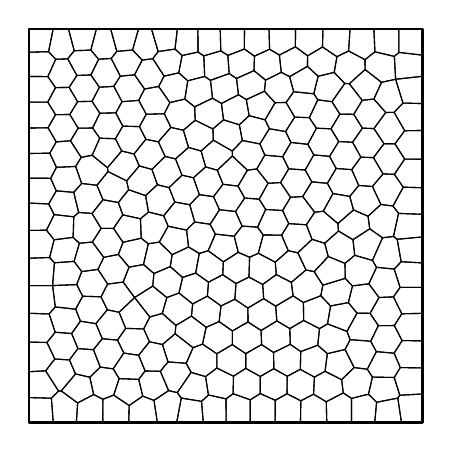
\begin{tikzpicture}[scale=5.0, line join=round]

    % Domain.
    \draw[thick]
        (0,0) -- (1,0) -- (1,1) -- (0,1) -- cycle;
    
    % Cells.
    \foreach \polygon in {
		{(0.85425003922567,0.89643441653084)--(0.89586440178401,0.86397550206595)--(0.93179591565974,0.87178722719166)--(0.92853152456159,0.92984144835401)--(0.87916498333343,0.94147386508211)--(0.85392976462248,0.92156728199569)},
		{(0.18771810493067,-3.3881317890172e-21)--(0.25391401123854,-3.3881317890172e-21)--(0.25495202735011,0.043060126990443)--(0.21564770756254,0.069547712690875)--(0.18841365337564,0.058974082408693)},
		{(0.46069118126695,0.50349277694441)--(0.47382843331691,0.4785102873257)--(0.52179006995416,0.4730630534635)--(0.54175966175634,0.49883733190863)--(0.52522632700706,0.53590345873871)--(0.48449791796453,0.54033710263574)},
		{(0.89586440178401,0.86397550206595)--(0.85425003922567,0.89643441653084)--(0.81412652870943,0.86044006877879)--(0.8469078244442,0.81818139289713)--(0.87656670190128,0.82155332306132)},
		{(0.27924818239616,0.81818065629307)--(0.29837945668825,0.78283012693449)--(0.34415098523973,0.78426441284968)--(0.35833086721755,0.81261322277255)--(0.32993659076441,0.85342577075569)--(0.29405320564213,0.84700245111173)},
		{(0.54825555593111,0.57012375522786)--(0.58511690372941,0.56717575448035)--(0.6078458583614,0.60745456688941)--(0.57911410039657,0.64400457256255)--(0.55522230074978,0.64079675988047)--(0.53145922569283,0.60048582390892)},
		{(0.75155122714303,0.45520354148788)--(0.71948017826896,0.46520877074272)--(0.68335038360887,0.43097101236)--(0.70411047302286,0.38738696947992)--(0.72487666360992,0.38310396889508)--(0.76069650918738,0.42157085669881)},
		{(1.0,0.13864853214086)--(1.0,0.20744236380782)--(0.94818852459171,0.20799608502154)--(0.92797517251722,0.17598351189508)--(0.94362287746415,0.13944429534222)},
		{(0.8033827921932,0.18539710036067)--(0.75834503615388,0.17482210021649)--(0.75251356236802,0.12990007449404)--(0.79471164658847,0.10863092922377)--(0.82620464554246,0.13947155936476)},
		{(0.4667078469644,0.82373134587444)--(0.48934878670151,0.8103216046155)--(0.53258107081332,0.83233041185575)--(0.52765335148172,0.87381602214682)--(0.50907339646748,0.88627112000211)--(0.46147900235953,0.86902677597484)},
		{(1.0,0.59618875232451)--(1.0,0.6685510395906)--(0.95479267230257,0.66901725367716)--(0.92856878499515,0.63026580110963)--(0.95111894205677,0.59770320908139)},
		{(0.13443535901413,0.38326874939109)--(0.17579566698028,0.38882213157283)--(0.19047663562534,0.41937680908285)--(0.16155799562524,0.45836208751523)--(0.12854897958594,0.45522094824717)--(0.11503831035262,0.40917956442035)},
		{(0.53258107081332,0.83233041185575)--(0.48934878670151,0.8103216046155)--(0.49465541123252,0.76875451290326)--(0.53482092578455,0.75611785700562)--(0.55977852971178,0.77929576825198)--(0.55254961833136,0.82022568195288)},
		{(0.93179591565974,0.87178722719166)--(0.89586440178401,0.86397550206595)--(0.87656670190128,0.82155332306132)--(0.90668243771493,0.7874342072159)--(0.92796840606646,0.78765373276468)--(0.95040016533829,0.8113845140569)},
		{(0.36099484423192,0.74953696953823)--(0.34415098523973,0.78426441284968)--(0.29837945668825,0.78283012693449)--(0.2810830330724,0.75150619104543)--(0.2972765889521,0.71917187517381)--(0.32921107558746,0.7129096055981)},
		{(0.75834503615388,0.17482210021649)--(0.8033827921932,0.18539710036067)--(0.81622015262675,0.21045839792942)--(0.80824759013231,0.23132377601912)--(0.75877513888218,0.25041903711036)--(0.73844198322554,0.23839333940357)--(0.73396253718825,0.19620715050472)},
		{(0.62580317947086,0.0)--(0.69009496466224,0.0)--(0.69093477167147,0.055029556276006)--(0.65583290404623,0.073057790939318)--(0.62609669905901,0.056317670448247)},
		{(0.16479707840632,0.070916402062561)--(0.15507236057507,0.11495364438172)--(0.11869083722568,0.12331318759982)--(0.082385023923309,0.08026817808489)--(0.12408344363776,0.049593512201291)},
		{(0.54796011614031,1.0)--(0.48624566349497,1.0)--(0.48768098362247,0.94390301390368)--(0.50562584380716,0.93230038069912)--(0.54749947141357,0.94847310619784)},
		{(0.0,0.87891212139603)--(0.0,0.81382219367018)--(0.048171703260738,0.81384095570995)--(0.068000373574546,0.85057346687317)--(0.048359260630003,0.87855452872397)},
		{(0.95111894205677,0.59770320908139)--(0.92856878499515,0.63026580110963)--(0.8997339716535,0.63145416032189)--(0.87286426402635,0.59942613356392)--(0.89434971804251,0.55372547045883)--(0.92513669999935,0.5497860359374)},
		{(0.58511690372941,0.56717575448035)--(0.54825555593111,0.57012375522786)--(0.52522632700706,0.53590345873871)--(0.54175966175634,0.49883733190863)--(0.58102901001086,0.49614372547287)--(0.60175292768188,0.54102427182116)},
		{(3.3881317890172e-21,0.48780488572576)--(3.3881317890172e-21,0.41726564361448)--(0.052930099930436,0.41900543205638)--(0.064301169368863,0.46400707949415)--(0.045009470508999,0.48830689077937)},
		{(0.6522183726502,0.73895492720754)--(0.66584623220444,0.71131379229515)--(0.70882555448055,0.70648501074389)--(0.73051520520934,0.74752402808075)--(0.71258718077491,0.77415210371676)--(0.67541502781966,0.77560643574924)},
		{(0.59134432077807,0.19791487356964)--(0.62179061371619,0.17762764002656)--(0.66419984777725,0.19854875567516)--(0.66309796491483,0.23849886213738)--(0.6301000264638,0.25799209769267)--(0.59015598113246,0.23352371297393)},
		{(0.6078458583614,0.60745456688941)--(0.58511690372941,0.56717575448035)--(0.60175292768188,0.54102427182116)--(0.64468512206964,0.53837264644062)--(0.66494994003711,0.57186511269423)--(0.63954194898965,0.60940748378258)},
		{(0.7676751337491,0.74583281628521)--(0.78721299869904,0.71362239948621)--(0.82243558748735,0.71177404873569)--(0.84741926255531,0.74765649645098)--(0.8254038773113,0.78265830063062)--(0.79008623988729,0.78332311457552)},
		{(1.0,0.27714487713853)--(1.0,0.34316024035882)--(0.94311016160597,0.34302386705696)--(0.92627492383454,0.31911009551348)--(0.94741027981677,0.27617218722635)},
		{(0.6448350817643,0.67492046909927)--(0.66584623220444,0.71131379229515)--(0.6522183726502,0.73895492720754)--(0.61107250672688,0.74609996956477)--(0.58706408486718,0.70748329920842)--(0.59948476563896,0.67903915888523)},
		{(0.12220801165102,0.8813274036494)--(0.15757612080664,0.88276755642973)--(0.17759427791703,0.92265385824788)--(0.1575074656902,0.94578507825734)--(0.11546233326623,0.94421738417224)--(0.098797758371704,0.92362834317442)},
		{(0.54749947141357,0.94847310619784)--(0.50562584380716,0.93230038069912)--(0.50907339646748,0.88627112000211)--(0.52765335148172,0.87381602214682)--(0.57203200130389,0.89369499299549)--(0.57329447927375,0.93051498260792)},
		{(0.046229275639784,0.20319958349053)--(0.066121044671373,0.16128414351659)--(0.10320019116217,0.15882274425156)--(0.12484045781112,0.18775613579888)--(0.10888402488129,0.22604332079741)--(0.067203909179232,0.22918549929927)},
		{(0.94741027981677,0.27617218722635)--(0.92627492383454,0.31911009551348)--(0.88955020154899,0.31746136795586)--(0.86684437077808,0.27724953418331)--(0.88800240926245,0.24600186764561)--(0.92849761864215,0.24622721422168)},
		{(0.29136664820548,0.40122013679363)--(0.31784166808222,0.3784263494454)--(0.35938161758489,0.39592703144047)--(0.36409887157382,0.42618059218067)--(0.33135704767331,0.45813172426122)--(0.30359722162812,0.45405655723607)},
		{(0.31784166808222,0.3784263494454)--(0.29136664820548,0.40122013679363)--(0.25467216949232,0.39455830390227)--(0.2397687466022,0.35659581930058)--(0.26879377464111,0.31732232857312)--(0.3148733693912,0.34650477303771)},
		{(0.25391401123854,0.0)--(0.32664090672374,0.0)--(0.31797314641036,0.056056876108632)--(0.28941427268521,0.067003139863361)--(0.25495202735011,0.043060126990443)},
		{(0.92796840606646,0.78765373276468)--(0.90668243771493,0.7874342072159)--(0.87661897827701,0.74645498479262)--(0.90222615557255,0.70812321089666)--(0.92991620758179,0.70778420599065)--(0.95486119233134,0.7410307208887)},
		{(0.74710259216562,1.0)--(0.67736412417465,1.0)--(0.67729872721556,0.95421974461399)--(0.7082404923537,0.93129500210585)--(0.74605601097852,0.95379023437869)},
		{(0.3148733693912,0.34650477303771)--(0.26879377464111,0.31732232857312)--(0.30743092622838,0.26806991131906)--(0.33917096257844,0.27706726209233)--(0.35061623605141,0.31730411300191)},
		{(0.8469078244442,0.81818139289713)--(0.81412652870943,0.86044006877879)--(0.8026036806208,0.86115274711927)--(0.77017170923042,0.81474409935631)--(0.79008623988729,0.78332311457552)--(0.8254038773113,0.78265830063062)},
		{(0.45556558902292,0.4361728753833)--(0.43310361858582,0.42930669386669)--(0.42384173347292,0.37956368907541)--(0.45647752499912,0.35634658702822)--(0.49268091669652,0.37542555734387)--(0.49424556399895,0.40811195113528)},
		{(0.48345432090595,0.25621307588729)--(0.45055240109438,0.24177725497777)--(0.44127073758729,0.19904467394915)--(0.4776093605498,0.17459394562545)--(0.51694240708711,0.19782265271774)--(0.51722538163216,0.23251064885303)},
		{(0.19047663562534,0.41937680908285)--(0.17579566698028,0.38882213157283)--(0.20032022729602,0.35158458773322)--(0.2397687466022,0.35659581930058)--(0.25467216949232,0.39455830390227)--(0.22756656734953,0.42689195969559)},
		{(0.42262574542254,0.76771375426766)--(0.46764389243995,0.74565115310262)--(0.49465541123252,0.76875451290326)--(0.48934878670151,0.8103216046155)--(0.4667078469644,0.82373134587444)--(0.42139137781863,0.80170132458699)},
		{(0.16095685473514,0.6788077579577)--(0.13316418183393,0.6733228975817)--(0.11914743271257,0.65033876654072)--(0.13428695258271,0.60716955768953)--(0.17319771716581,0.60247378054863)--(0.20128039004511,0.6374818910852)--(0.19984950030603,0.6471399563931)},
		{(0.72384227076444,0.67965033698535)--(0.70209954589213,0.64131332655495)--(0.71876436831641,0.61123524113896)--(0.75842856465024,0.60751735433328)--(0.78076047728658,0.64515661035686)--(0.76402955473388,0.67592741012559)},
		{(0.40572845164225,0.69863577383034)--(0.43761725779504,0.68954435491125)--(0.46869170660175,0.71707035726209)--(0.46764389243995,0.74565115310262)--(0.42262574542254,0.76771375426766)--(0.39263059535003,0.74223863901003)},
		{(0.80378817962939,0.36597492889705)--(0.82221880733978,0.34690064613188)--(0.86374843489741,0.35223124942516)--(0.88331577287452,0.39420496877405)--(0.87287789417251,0.41169585999104)--(0.82793947169247,0.4246902413447)--(0.80316479093177,0.40418178368694)},
		{(-3.3881317890172e-21,0.20419335883761)--(-3.3881317890172e-21,0.12896736835814)--(0.042863656064778,0.13118085741329)--(0.066121044671373,0.16128414351659)--(0.046229275639784,0.20319958349053)},
		{(0.86374843489741,0.35223124942516)--(0.82221880733978,0.34690064613188)--(0.81175871481672,0.30453478989315)--(0.83361794086063,0.2777065038937)--(0.86684437077808,0.27724953418331)--(0.88955020154899,0.31746136795586)},
		{(0.58783360786316,0.073462450074628)--(0.58807832348295,0.11692777651187)--(0.55098965776865,0.13744223929783)--(0.51988442908642,0.11752708217047)--(0.51911854393209,0.072969258959661)--(0.56266405065388,0.057545241211319)},
		{(0.40881039814549,0.55303665480546)--(0.37093258229203,0.55999562959625)--(0.34281455669062,0.52501304381112)--(0.35403157684083,0.49845963692288)--(0.4008413602106,0.4886415602741)--(0.42150463543288,0.50924989745564)},
		{(0.87876053524142,-3.3881317890172e-21)--(0.9466572855243,-3.3881317890172e-21)--(0.93730478749826,0.061973555988135)--(0.88344783577229,0.051364730957438)},
		{(0.51694240708711,0.19782265271774)--(0.4776093605498,0.17459394562545)--(0.47778697142604,0.13836567781697)--(0.51988442908642,0.11752708217047)--(0.55098965776865,0.13744223929783)--(0.55103111543584,0.17483695627742)},
		{(0.33917096257844,0.27706726209233)--(0.30743092622838,0.26806991131906)--(0.29174823815601,0.23759667152464)--(0.30670907561533,0.20504511217484)--(0.3395468429255,0.19806713436986)--(0.3717399593541,0.22545185598031)--(0.3735291806428,0.24650974243263)},
		{(0.068000373574546,0.85057346687317)--(0.048171703260738,0.81384095570995)--(0.067947467606083,0.78183427096966)--(0.10434440972917,0.78236701110505)--(0.12393548511197,0.81490273721698)--(0.10242480980474,0.85105546170517)},
		{(0.60175292768188,0.54102427182116)--(0.58102901001086,0.49614372547287)--(0.59546533027787,0.47633900221885)--(0.64222924982185,0.47580469795012)--(0.66025929037073,0.50512589355828)--(0.64468512206964,0.53837264644062)},
		{(0.0,0.81382219367018)--(0.0,0.74782145548499)--(0.048940574310007,0.74861162763832)--(0.067947467606083,0.78183427096966)--(0.048171703260738,0.81384095570995)},
		{(0.82793947169247,0.4246902413447)--(0.87287789417251,0.41169585999104)--(0.89848212160814,0.46911121720684)--(0.86603411169357,0.49195838682805)--(0.82341473259487,0.46422957239014)},
		{(0.57329447927375,0.93051498260792)--(0.57203200130389,0.89369499299549)--(0.6014211136318,0.86967584469896)--(0.64133725528727,0.88941288525035)--(0.63656591841046,0.93322822403677)--(0.61162597448809,0.94806119179528)},
		{(0.26879377464111,0.31732232857312)--(0.2397687466022,0.35659581930058)--(0.20032022729602,0.35158458773322)--(0.18356856224297,0.31925023590169)--(0.19936639593068,0.28628210047732)--(0.22941156618117,0.27991215520462)},
		{(0.70209954589213,0.64131332655495)--(0.72384227076444,0.67965033698535)--(0.70882555448055,0.70648501074389)--(0.66584623220444,0.71131379229515)--(0.6448350817643,0.67492046909927)--(0.66022881502927,0.64426892666792)},
		{(0.045009470508999,0.48830689077937)--(0.064301169368863,0.46400707949415)--(0.11270693375421,0.47017888928131)--(0.11429876669671,0.5223866891342)--(0.064480674796889,0.52803924453535)},
		{(0.082385023923309,0.08026817808489)--(0.11869083722568,0.12331318759982)--(0.10320019116217,0.15882274425156)--(0.066121044671373,0.16128414351659)--(0.042863656064778,0.13118085741329)--(0.075703605736403,0.079666468996901)},
		{(0.81602890949285,1.0)--(0.74710259216562,1.0)--(0.74605601097852,0.95379023437869)--(0.78273727312518,0.92909233483648)--(0.81231420735892,0.94357266810201)},
		{(0.41321524320541,0.27013213722296)--(0.45055240109438,0.24177725497777)--(0.48345432090595,0.25621307588729)--(0.48822927752933,0.29609331359553)--(0.45366849104597,0.32087462363446)--(0.41632511883173,0.30112363203544)},
		{(0.18045111173012,0.7854867957333)--(0.16066657494435,0.81580095825201)--(0.12393548511197,0.81490273721698)--(0.10434440972917,0.78236701110505)--(0.12535653588861,0.74746398987498)--(0.16207203537302,0.74797093164383)},
		{(0.79471164658847,0.10863092922377)--(0.75251356236802,0.12990007449404)--(0.72562285867184,0.11531212379474)--(0.72328473500472,0.07184460520266)--(0.75562242119361,0.052596005649806)--(0.79878740978037,0.075144411330181)},
		{(0.88800240926245,0.24600186764561)--(0.86684437077808,0.27724953418331)--(0.83361794086063,0.2777065038937)--(0.80824759013231,0.23132377601912)--(0.81622015262675,0.21045839792942)--(0.86841500362821,0.20639309881428)},
		{(0.18667012102422,0.21273971622346)--(0.1641846302661,0.18482385447381)--(0.18159732241283,0.14072049274371)--(0.21443922185002,0.13621332706864)--(0.24125029453435,0.17638003508631)--(0.22538658447158,0.20921134555963)},
		{(0.48822927752933,0.29609331359553)--(0.48345432090595,0.25621307588729)--(0.51722538163216,0.23251064885303)--(0.55694631100662,0.25542410938362)--(0.55643254631388,0.2907421720222)--(0.52342194374864,0.31297996773677)},
		{(0.9466572855243,0.0)--(1.0,0.0)--(1.0,0.072349655886911)--(0.94231273845427,0.069179857769253)--(0.93730478749826,0.061973555988135)},
		{(0.69009496466224,0.0)--(0.75691436011856,0.0)--(0.75562242119361,0.052596005649806)--(0.72328473500472,0.07184460520266)--(0.69093477167147,0.055029556276006)},
		{(0.92513669999935,0.5497860359374)--(0.89434971804251,0.55372547045883)--(0.86177092785854,0.52388809186533)--(0.86603411169357,0.49195838682805)--(0.89848212160814,0.46911121720684)--(0.92638879819591,0.47245043135597)--(0.93921911048369,0.53108301386062)},
		{(0.58303014229697,0.42983883370655)--(0.62603489789952,0.40722151380765)--(0.65912958634453,0.43645717996931)--(0.64222924982185,0.47580469795012)--(0.59546533027787,0.47633900221885)},
		{(0.53482092578455,0.75611785700562)--(0.49465541123252,0.76875451290326)--(0.46764389243995,0.74565115310262)--(0.46869170660175,0.71707035726209)--(0.5168888793673,0.68950322607661)--(0.54240662087538,0.71631968138848)},
		{(0.73396253718825,0.19620715050472)--(0.73844198322554,0.23839333940357)--(0.6982118429573,0.25915924958796)--(0.66309796491483,0.23849886213738)--(0.66419984777725,0.19854875567516)--(0.69080439876367,0.18004295875834)},
		{(0.3964139638074,0.82140177892316)--(0.42139137781863,0.80170132458699)--(0.4667078469644,0.82373134587444)--(0.46147900235953,0.86902677597484)--(0.44682618977808,0.87890590607107)--(0.40380900723045,0.86794262496174)},
		{(0.71948017826896,0.46520877074272)--(0.75155122714303,0.45520354148788)--(0.78659109738853,0.48630693082959)--(0.78523982186898,0.50522717647608)--(0.74801067811641,0.53670714528273)--(0.72617338877445,0.5339069218775)--(0.70508932262291,0.50213889793751)},
		{(1.0,0.40531466621466)--(1.0,0.4713492626969)--(0.93578475761593,0.46525451512957)--(0.94577206391554,0.40830295762278)},
		{(0.49424556399895,0.40811195113528)--(0.49268091669652,0.37542555734387)--(0.52631827451913,0.35293114336325)--(0.55925462231903,0.36930019453421)--(0.56089380540685,0.41958328971554)--(0.53195309307421,0.43218679146806)},
		{(0.75842856465024,0.60751735433328)--(0.71876436831641,0.61123524113896)--(0.69582694358102,0.57390823390226)--(0.72617338877445,0.5339069218775)--(0.74801067811641,0.53670714528273)--(0.7725801474678,0.58161128576417)},
		{(0.16071684588932,0.53087731810653)--(0.18379875607524,0.49284037194156)--(0.21517425621597,0.49312969768415)--(0.23878085692852,0.5274365480845)--(0.22749482706973,0.55866500918541)--(0.1884858402807,0.56577668163639)},
		{(0.62609669905901,0.056317670448247)--(0.65583290404623,0.073057790939318)--(0.65653800226594,0.1174584126321)--(0.62233288276887,0.13662440642725)--(0.58807832348295,0.11692777651187)--(0.58783360786316,0.073462450074628)},
		{(0.70779681735954,0.9045247946079)--(0.66245732263949,0.87832950351389)--(0.67288306419903,0.84002051822184)--(0.72393450897079,0.83484744653536)--(0.73499829718929,0.87932646606082)},
		{(0.27926124224363,0.10950934165904)--(0.29537496982985,0.13085587687186)--(0.27901501669798,0.17072982451914)--(0.24125029453435,0.17638003508631)--(0.21443922185002,0.13621332706864)--(0.22963746541835,0.11143057237846)},
		{(0.13121683661145,0.25729401883088)--(0.10888402488129,0.22604332079741)--(0.12484045781112,0.18775613579888)--(0.1641846302661,0.18482385447381)--(0.18667012102422,0.21273971622346)--(0.17049581096501,0.25107753503047)},
		{(0.17944512520274,0.85162693982689)--(0.16066657494435,0.81580095825201)--(0.18045111173012,0.7854867957333)--(0.22103048018019,0.78651356159867)--(0.23693825536183,0.81483437610826)--(0.21599836129715,0.8537507465213)},
		{(0.27881902020782,1.0)--(0.20788364016602,1.0)--(0.22355231567875,0.9425370168425)--(0.26357734406753,0.94611821656284)},
		{(0.35833086721755,0.81261322277255)--(0.34415098523973,0.78426441284968)--(0.36099484423192,0.74953696953823)--(0.39263059535003,0.74223863901003)--(0.42262574542254,0.76771375426766)--(0.42139137781863,0.80170132458699)--(0.3964139638074,0.82140177892316)},
		{(0.44682618977808,0.87890590607107)--(0.46147900235953,0.86902677597484)--(0.50907339646748,0.88627112000211)--(0.50562584380716,0.93230038069912)--(0.48768098362247,0.94390301390368)--(0.44461210776746,0.93114469490456)},
		{(0.62179061371619,0.17762764002656)--(0.59134432077807,0.19791487356964)--(0.55103111543584,0.17483695627742)--(0.55098965776865,0.13744223929783)--(0.58807832348295,0.11692777651187)--(0.62233288276887,0.13662440642725)},
		{(0.062141427440111,0.0)--(0.12086280595219,0.0)--(0.12408344363776,0.049593512201291)--(0.082385023923309,0.08026817808489)--(0.075703605736403,0.079666468996901)--(0.057432907805433,0.061633776598765)},
		{(1.0,0.80995771423665)--(1.0,0.87927974379184)--(0.93179591565974,0.87178722719166)--(0.95040016533829,0.8113845140569)},
		{(0.61014031960486,1.0)--(0.54796011614031,1.0)--(0.54749947141357,0.94847310619784)--(0.57329447927375,0.93051498260792)--(0.61162597448809,0.94806119179528)},
		{(0.29537496982985,0.13085587687186)--(0.27926124224363,0.10950934165904)--(0.28941427268521,0.067003139863361)--(0.31797314641036,0.056056876108632)--(0.35531678732075,0.080945822003257)--(0.33405941380179,0.12995050482729)},
		{(0.40380900723045,0.86794262496174)--(0.44682618977808,0.87890590607107)--(0.44461210776746,0.93114469490456)--(0.42988980094971,0.94083978517576)--(0.38940217585767,0.93210311038586)--(0.38086790012693,0.88800543604605)},
		{(0.83804769068055,0.60206387134622)--(0.82026544528165,0.64220165339116)--(0.78076047728658,0.64515661035686)--(0.75842856465024,0.60751735433328)--(0.7725801474678,0.58161128576417)--(0.81528699207023,0.57426573447145)},
		{(0.36409887157382,0.42618059218067)--(0.35938161758489,0.39592703144047)--(0.39067966361553,0.36833889488444)--(0.42384173347292,0.37956368907541)--(0.43310361858582,0.42930669386669)--(0.40579674578015,0.44574356633011)},
		{(0.75251356236802,0.12990007449404)--(0.75834503615388,0.17482210021649)--(0.73396253718825,0.19620715050472)--(0.69080439876367,0.18004295875834)--(0.68963872659298,0.13491147467802)--(0.72562285867184,0.11531212379474)},
		{(0.3115319648963,1.0)--(0.27881902020782,1.0)--(0.26357734406753,0.94611821656284)--(0.28803140334348,0.92041462029335)--(0.31507194021601,0.92393461049221)--(0.32854621162978,0.94212845296294)},
		{(0.22756656734953,0.42689195969559)--(0.25467216949232,0.39455830390227)--(0.29136664820548,0.40122013679363)--(0.30359722162812,0.45405655723607)--(0.28553237032144,0.46803328823195)--(0.2392584550794,0.45765426159839)},
		{(0.12854897958594,0.45522094824717)--(0.16155799562524,0.45836208751523)--(0.18379875607524,0.49284037194156)--(0.16071684588932,0.53087731810653)--(0.12664846716677,0.5334559271228)--(0.11429876669671,0.5223866891342)--(0.11270693375421,0.47017888928131)},
		{(0.2392584550794,0.45765426159839)--(0.28553237032144,0.46803328823195)--(0.28370743180877,0.51741991683203)--(0.23878085692852,0.5274365480845)--(0.21517425621597,0.49312969768415)},
		{(0.43761725779504,0.68954435491125)--(0.40572845164225,0.69863577383034)--(0.3726605346977,0.66948370884871)--(0.38907475232691,0.62817843545602)--(0.41828971625287,0.62151554658588)--(0.4492453699447,0.6492517447276)},
		{(0.2810830330724,0.75150619104543)--(0.29837945668825,0.78283012693449)--(0.27924818239616,0.81818065629307)--(0.23693825536183,0.81483437610826)--(0.22103048018019,0.78651356159867)--(0.23871720266627,0.75268530383301)},
		{(0.55254961833136,0.82022568195288)--(0.55977852971178,0.77929576825198)--(0.60024521684276,0.76866041089786)--(0.62551411722217,0.81216208674502)--(0.59850408020428,0.84138680533318)},
		{(0.0,0.68315603033768)--(0.0,0.62049393976181)--(0.055438075863687,0.62017108498914)--(0.070258679106007,0.6480147338871)--(0.053326266337507,0.68401352055842)},
		{(0.81975710861705,0.0)--(0.87876053524142,0.0)--(0.88344783577229,0.051364730957438)--(0.86278630049968,0.071825742170177)--(0.81973221992345,0.061234551000413)},
		{(0.62603489789952,0.40722151380765)--(0.58303014229697,0.42983883370655)--(0.56089380540685,0.41958328971554)--(0.55925462231903,0.36930019453421)--(0.59418507702959,0.3506021392863)--(0.62869156359708,0.37564646622078)},
		{(1.0,0.74173664947945)--(1.0,0.80995771423665)--(0.95040016533829,0.8113845140569)--(0.92796840606646,0.78765373276468)--(0.95486119233134,0.7410307208887)},
		{(0.55925462231903,0.36930019453421)--(0.52631827451913,0.35293114336325)--(0.52342194374864,0.31297996773677)--(0.55643254631388,0.2907421720222)--(0.59662487164694,0.3145409996043)--(0.59418507702959,0.3506021392863)},
		{(0.74175580910786,0.32193793817147)--(0.76662829848874,0.29598170726442)--(0.81175871481672,0.30453478989315)--(0.82221880733978,0.34690064613188)--(0.80378817962939,0.36597492889705)--(0.74689896156538,0.34874601481063)},
		{(0.0,0.27737113686155)--(0.0,0.20419335883761)--(0.046229275639784,0.20319958349053)--(0.067203909179232,0.22918549929927)--(0.051718536330769,0.27567930595858)},
		{(0.73051520520934,0.74752402808075)--(0.70882555448055,0.70648501074389)--(0.72384227076444,0.67965033698535)--(0.76402955473388,0.67592741012559)--(0.78721299869904,0.71362239948621)--(0.7676751337491,0.74583281628521)},
		{(0.4295746579052,1.0)--(0.37738581311672,1.0)--(0.37144195771888,0.9484016144798)--(0.38940217585767,0.93210311038586)--(0.42988980094971,0.94083978517576)},
		{(0.63954194898965,0.60940748378258)--(0.66494994003711,0.57186511269423)--(0.69582694358102,0.57390823390226)--(0.71876436831641,0.61123524113896)--(0.70209954589213,0.64131332655495)--(0.66022881502927,0.64426892666792)},
		{(0.32854621162978,0.94212845296294)--(0.31507194021601,0.92393461049221)--(0.34371927678055,0.87978002819975)--(0.38086790012693,0.88800543604605)--(0.38940217585767,0.93210311038586)--(0.37144195771888,0.9484016144798)},
		{(0.13428695258271,0.60716955768953)--(0.11914743271257,0.65033876654072)--(0.070258679106007,0.6480147338871)--(0.055438075863687,0.62017108498914)--(0.069870515394689,0.58838904931392)--(0.1142462918977,0.58453667552324)},
		{(0.4008413602106,0.4886415602741)--(0.35403157684083,0.49845963692288)--(0.33135704767331,0.45813172426122)--(0.36409887157382,0.42618059218067)--(0.40579674578015,0.44574356633011)},
		{(0.32675979969901,0.60391025172265)--(0.35634139240662,0.596400374444)--(0.38907475232691,0.62817843545602)--(0.3726605346977,0.66948370884871)--(0.346281018991,0.6757489893598)--(0.31269853923641,0.64283449548429)},
		{(0.26868711038678,0.88306687933854)--(0.29405320564213,0.84700245111173)--(0.32993659076441,0.85342577075569)--(0.34371927678055,0.87978002819975)--(0.31507194021601,0.92393461049221)--(0.28803140334348,0.92041462029335)},
		{(0.49268091669652,0.37542555734387)--(0.45647752499912,0.35634658702822)--(0.45366849104597,0.32087462363446)--(0.48822927752933,0.29609331359553)--(0.52342194374864,0.31297996773677)--(0.52631827451913,0.35293114336325)},
		{(0.62711122329781,0.29544173620704)--(0.6301000264638,0.25799209769267)--(0.66309796491483,0.23849886213738)--(0.6982118429573,0.25915924958796)--(0.69748885459586,0.30470519395951)--(0.67131627431904,0.32152790090721)},
		{(0.41721813578252,0.18994863971108)--(0.3717399593541,0.22545185598031)--(0.3395468429255,0.19806713436986)--(0.35366703457182,0.15385412246116)--(0.39991040110177,0.15038593580758)},
		{(0.69748885459586,0.30470519395951)--(0.6982118429573,0.25915924958796)--(0.73844198322554,0.23839333940357)--(0.75877513888218,0.25041903711036)--(0.76662829848874,0.29598170726442)--(0.74175580910786,0.32193793817147)},
		{(0.0,0.34764884396329)--(0.0,0.27737113686155)--(0.051718536330769,0.27567930595858)--(0.067346333031576,0.29344768027072)--(0.060466430455996,0.34778571497783)},
		{(0.71258718077491,0.77415210371676)--(0.73051520520934,0.74752402808075)--(0.7676751337491,0.74583281628521)--(0.79008623988729,0.78332311457552)--(0.77017170923042,0.81474409935631)--(0.73398098170073,0.81956342710585)},
		{(0.53145922569283,0.60048582390892)--(0.55522230074978,0.64079675988047)--(0.51712977044261,0.67696805458597)--(0.47884504334911,0.64077458810679)--(0.49328320152969,0.60502709039101)},
		{(0.067203909179232,0.22918549929927)--(0.10888402488129,0.22604332079741)--(0.13121683661145,0.25729401883088)--(0.11900271614634,0.28776047187196)--(0.067346333031576,0.29344768027072)--(0.051718536330769,0.27567930595858)},
		{(0.47382843331691,0.4785102873257)--(0.46069118126695,0.50349277694441)--(0.42150463543288,0.50924989745564)--(0.4008413602106,0.4886415602741)--(0.40579674578015,0.44574356633011)--(0.43310361858582,0.42930669386669)--(0.45556558902292,0.4361728753833)},
		{(0.18841365337564,0.058974082408693)--(0.21564770756254,0.069547712690875)--(0.22963746541835,0.11143057237846)--(0.21443922185002,0.13621332706864)--(0.18159732241283,0.14072049274371)--(0.15507236057507,0.11495364438172)--(0.16479707840632,0.070916402062561)},
		{(0.064480674796889,0.52803924453535)--(0.11429876669671,0.5223866891342)--(0.12664846716677,0.5334559271228)--(0.1142462918977,0.58453667552324)--(0.069870515394689,0.58838904931392)--(0.050553838541673,0.55498108555111)},
		{(0.075703605736403,0.079666468996901)--(0.042863656064778,0.13118085741329)--(0.0,0.12896736835814)--(0.0,0.063307937351908)--(0.057432907805433,0.061633776598765)},
		{(0.16155799562524,0.45836208751523)--(0.19047663562534,0.41937680908285)--(0.22756656734953,0.42689195969559)--(0.2392584550794,0.45765426159839)--(0.21517425621597,0.49312969768415)--(0.18379875607524,0.49284037194156)},
		{(0.70508932262291,0.50213889793751)--(0.72617338877445,0.5339069218775)--(0.69582694358102,0.57390823390226)--(0.66494994003711,0.57186511269423)--(0.64468512206964,0.53837264644062)--(0.66025929037073,0.50512589355828)},
		{(0.062047620960928,1.0)--(0.0,1.0)--(0.0,0.94037953523977)--(0.050251178415103,0.94181842156166)},
		{(0.48449791796453,0.54033710263574)--(0.52522632700706,0.53590345873871)--(0.54825555593111,0.57012375522786)--(0.53145922569283,0.60048582390892)--(0.49328320152969,0.60502709039101)--(0.46920358859454,0.57357787837279)},
		{(0.44899755850348,0.11653849264436)--(0.41225828930296,0.12732335971011)--(0.37721649474944,0.075881478589466)--(0.38732960280625,0.062032946778208)--(0.43881426541099,0.053692099847969)--(0.45632958303313,0.069926020987252)},
		{(0.87286426402635,0.59942613356392)--(0.8997339716535,0.63145416032189)--(0.87555242086899,0.67275329239539)--(0.84357438884983,0.67391708539654)--(0.82026544528165,0.64220165339116)--(0.83804769068055,0.60206387134622)},
		{(0.30409981126291,0.53450401682049)--(0.34281455669062,0.52501304381112)--(0.37093258229203,0.55999562959625)--(0.35634139240662,0.596400374444)--(0.32675979969901,0.60391025172265)--(0.29666607558037,0.57631284104634)},
		{(1.0,0.34316024035882)--(1.0,0.40531466621466)--(0.94577206391554,0.40830295762278)--(0.9281810754791,0.38965849560362)--(0.94311016160597,0.34302386705696)},
		{(0.76402955473388,0.67592741012559)--(0.78076047728658,0.64515661035686)--(0.82026544528165,0.64220165339116)--(0.84357438884983,0.67391708539654)--(0.82243558748735,0.71177404873569)--(0.78721299869904,0.71362239948621)},
		{(0.17579566698028,0.38882213157283)--(0.13443535901413,0.38326874939109)--(0.12173675236714,0.35018831490272)--(0.13683152341573,0.32071464651463)--(0.18356856224297,0.31925023590169)--(0.20032022729602,0.35158458773322)},
		{(0.3735291806428,0.24650974243263)--(0.3717399593541,0.22545185598031)--(0.41721813578252,0.18994863971108)--(0.44127073758729,0.19904467394915)--(0.45055240109438,0.24177725497777)--(0.41321524320541,0.27013213722296)},
		{(0.67288306419903,0.84002051822184)--(0.66245732263949,0.87832950351389)--(0.64133725528727,0.88941288525035)--(0.6014211136318,0.86967584469896)--(0.59850408020428,0.84138680533318)--(0.62551411722217,0.81216208674502)--(0.65360013904418,0.81284053928524)},
		{(0.67541502781966,0.77560643574924)--(0.71258718077491,0.77415210371676)--(0.73398098170073,0.81956342710585)--(0.72393450897079,0.83484744653536)--(0.67288306419903,0.84002051822184)--(0.65360013904418,0.81284053928524)},
		{(1.0,0.6685510395906)--(1.0,0.74173664947945)--(0.95486119233134,0.7410307208887)--(0.92991620758179,0.70778420599065)--(0.95479267230257,0.66901725367716)},
		{(0.44317153028203,0.0)--(0.50131719775238,0.0)--(0.5008772470016,0.060016255794406)--(0.45632958303313,0.069926020987252)--(0.43881426541099,0.053692099847969)},
		{(0.87555242086899,0.67275329239539)--(0.8997339716535,0.63145416032189)--(0.92856878499515,0.63026580110963)--(0.95479267230257,0.66901725367716)--(0.92991620758179,0.70778420599065)--(0.90222615557255,0.70812321089666)},
		{(0.49328320152969,0.60502709039101)--(0.47884504334911,0.64077458810679)--(0.4492453699447,0.6492517447276)--(0.41828971625287,0.62151554658588)--(0.43326080099448,0.57871286162786)--(0.46920358859454,0.57357787837279)},
		{(0.20128039004511,0.6374818910852)--(0.17319771716581,0.60247378054863)--(0.1884858402807,0.56577668163639)--(0.22749482706973,0.55866500918541)--(0.25358087930606,0.59118363917895)--(0.24844604548202,0.61354454448507)},
		{(0.55522230074978,0.64079675988047)--(0.57911410039657,0.64400457256255)--(0.59948476563896,0.67903915888523)--(0.58706408486718,0.70748329920842)--(0.54240662087538,0.71631968138848)--(0.5168888793673,0.68950322607661)--(0.51712977044261,0.67696805458597)},
		{(0.15757612080664,0.88276755642973)--(0.12220801165102,0.8813274036494)--(0.10242480980474,0.85105546170517)--(0.12393548511197,0.81490273721698)--(0.16066657494435,0.81580095825201)--(0.17944512520274,0.85162693982689)},
		{(0.93995458302419,1.0)--(0.87659264470874,1.0)--(0.87916498333343,0.94147386508211)--(0.92853152456159,0.92984144835401)--(0.94021694842497,0.93989047442232)},
		{(0.59134432077807,0.19791487356964)--(0.59015598113246,0.23352371297393)--(0.55694631100662,0.25542410938362)--(0.51722538163216,0.23251064885303)--(0.51694240708711,0.19782265271774)--(0.55103111543584,0.17483695627742)},
		{(0.54175966175634,0.49883733190863)--(0.52179006995416,0.4730630534635)--(0.53195309307421,0.43218679146806)--(0.56089380540685,0.41958328971554)--(0.58303014229697,0.42983883370655)--(0.59546533027787,0.47633900221885)--(0.58102901001086,0.49614372547287)},
		{(0.59662487164694,0.3145409996043)--(0.55643254631388,0.2907421720222)--(0.55694631100662,0.25542410938362)--(0.59015598113246,0.23352371297393)--(0.6301000264638,0.25799209769267)--(0.62711122329781,0.29544173620704)},
		{(0.13316418183393,0.6733228975817)--(0.16095685473514,0.6788077579577)--(0.18015350057158,0.72208999850187)--(0.16207203537302,0.74797093164383)--(0.12535653588861,0.74746398987498)--(0.10592634028005,0.71552645144617)},
		{(0.68335038360887,0.43097101236)--(0.71948017826896,0.46520877074272)--(0.70508932262291,0.50213889793751)--(0.66025929037073,0.50512589355828)--(0.64222924982185,0.47580469795012)--(0.65912958634453,0.43645717996931)},
		{(1.0,0.20744236380782)--(1.0,0.27714487713853)--(0.94741027981677,0.27617218722635)--(0.92849761864215,0.24622721422168)--(0.94818852459171,0.20799608502154)},
		{(0.32921107558746,0.7129096055981)--(0.2972765889521,0.71917187517381)--(0.26740740311493,0.68193158936864)--(0.28082415417707,0.65156735848059)--(0.31269853923641,0.64283449548429)--(0.346281018991,0.6757489893598)},
		{(0.13683152341573,0.32071464651463)--(0.12173675236714,0.35018831490272)--(0.060466430455996,0.34778571497783)--(0.067346333031576,0.29344768027072)--(0.11900271614634,0.28776047187196)},
		{(0.41828971625287,0.62151554658588)--(0.38907475232691,0.62817843545602)--(0.35634139240662,0.596400374444)--(0.37093258229203,0.55999562959625)--(0.40881039814549,0.55303665480546)--(0.43326080099448,0.57871286162786)},
		{(0.35938161758489,0.39592703144047)--(0.31784166808222,0.3784263494454)--(0.3148733693912,0.34650477303771)--(0.35061623605141,0.31730411300191)--(0.38148175159146,0.32874361472468)--(0.39067966361553,0.36833889488444)},
		{(0.21599836129715,0.8537507465213)--(0.23693825536183,0.81483437610826)--(0.27924818239616,0.81818065629307)--(0.29405320564213,0.84700245111173)--(0.26868711038678,0.88306687933854)--(0.23253327749736,0.87956601154367)},
		{(1.0,0.4713492626969)--(1.0,0.52869431793065)--(0.93921911048369,0.53108301386062)--(0.92638879819591,0.47245043135597)--(0.93578475761593,0.46525451512957)},
		{(0.46069118126695,0.50349277694441)--(0.48449791796453,0.54033710263574)--(0.46920358859454,0.57357787837279)--(0.43326080099448,0.57871286162786)--(0.40881039814549,0.55303665480546)--(0.42150463543288,0.50924989745564)},
		{(0.32675979969901,0.60391025172265)--(0.31269853923641,0.64283449548429)--(0.28082415417707,0.65156735848059)--(0.24844604548202,0.61354454448507)--(0.25358087930606,0.59118363917895)--(0.29666607558037,0.57631284104634)},
		{(0.39991040110177,0.15038593580758)--(0.35366703457182,0.15385412246116)--(0.33405941380179,0.12995050482729)--(0.35531678732075,0.080945822003257)--(0.37721649474944,0.075881478589466)--(0.41225828930296,0.12732335971011)},
		{(0.58706408486718,0.70748329920842)--(0.61107250672688,0.74609996956477)--(0.60024521684276,0.76866041089786)--(0.55977852971178,0.77929576825198)--(0.53482092578455,0.75611785700562)--(0.54240662087538,0.71631968138848)},
		{(0.32664090672374,0.0)--(0.37568010651516,0.0)--(0.38732960280625,0.062032946778208)--(0.37721649474944,0.075881478589466)--(0.35531678732075,0.080945822003257)--(0.31797314641036,0.056056876108632)},
		{(0.23253327749736,0.87956601154367)--(0.26868711038678,0.88306687933854)--(0.28803140334348,0.92041462029335)--(0.26357734406753,0.94611821656284)--(0.22355231567875,0.9425370168425)--(0.20928345132573,0.92462125215238)},
		{(0.41632511883173,0.30112363203544)--(0.45366849104597,0.32087462363446)--(0.45647752499912,0.35634658702822)--(0.42384173347292,0.37956368907541)--(0.39067966361553,0.36833889488444)--(0.38148175159146,0.32874361472468)},
		{(0.56244236799357,-3.3881317890172e-21)--(0.62580317947086,0.0)--(0.62609669905901,0.056317670448247)--(0.58783360786316,0.073462450074628)--(0.56266405065388,0.057545241211319)},
		{(0.86177092785854,0.52388809186533)--(0.89434971804251,0.55372547045883)--(0.87286426402635,0.59942613356392)--(0.83804769068055,0.60206387134622)--(0.81528699207023,0.57426573447145)--(0.82482223695715,0.53988966713661)},
		{(0.4776093605498,0.17459394562545)--(0.44127073758729,0.19904467394915)--(0.41721813578252,0.18994863971108)--(0.39991040110177,0.15038593580758)--(0.41225828930296,0.12732335971011)--(0.44899755850348,0.11653849264436)--(0.47778697142604,0.13836567781697)},
		{(0.28370743180877,0.51741991683203)--(0.28553237032144,0.46803328823195)--(0.30359722162812,0.45405655723607)--(0.33135704767331,0.45813172426122)--(0.35403157684083,0.49845963692288)--(0.34281455669062,0.52501304381112)--(0.30409981126291,0.53450401682049)},
		{(0.40572845164225,0.69863577383034)--(0.39263059535003,0.74223863901003)--(0.36099484423192,0.74953696953823)--(0.32921107558746,0.7129096055981)--(0.346281018991,0.6757489893598)--(0.3726605346977,0.66948370884871)},
		{(0.0,0.74782145548499)--(0.0,0.68315603033768)--(0.053326266337507,0.68401352055842)--(0.06969010714392,0.71272907966457)--(0.048940574310007,0.74861162763832)},
		{(0.19936639593068,0.28628210047732)--(0.18356856224297,0.31925023590169)--(0.13683152341573,0.32071464651463)--(0.11900271614634,0.28776047187196)--(0.13121683661145,0.25729401883088)--(0.17049581096501,0.25107753503047)},
		{(0.69080439876367,0.18004295875834)--(0.66419984777725,0.19854875567516)--(0.62179061371619,0.17762764002656)--(0.62233288276887,0.13662440642725)--(0.65653800226594,0.1174584126321)--(0.68963872659298,0.13491147467802)},
		{(0.87289838992927,0.11516892913653)--(0.85976319902919,0.1353796288881)--(0.82620464554246,0.13947155936476)--(0.79471164658847,0.10863092922377)--(0.79878740978037,0.075144411330181)--(0.81973221992345,0.061234551000413)--(0.86278630049968,0.071825742170177)},
		{(0.50131719775238,3.3881317890172e-21)--(0.56244236799357,3.3881317890172e-21)--(0.56266405065388,0.057545241211319)--(0.51911854393209,0.072969258959661)--(0.5008772470016,0.060016255794406)},
		{(0.7082404923537,0.93129500210585)--(0.67729872721556,0.95421974461399)--(0.63656591841046,0.93322822403677)--(0.64133725528727,0.88941288525035)--(0.66245732263949,0.87832950351389)--(0.70779681735954,0.9045247946079)},
		{(0.29174823815601,0.23759667152464)--(0.30743092622838,0.26806991131906)--(0.26879377464111,0.31732232857312)--(0.22941156618117,0.27991215520462)--(0.24607087417752,0.23914243785724)},
		{(0.82482223695715,0.53988966713661)--(0.81528699207023,0.57426573447145)--(0.7725801474678,0.58161128576417)--(0.74801067811641,0.53670714528273)--(0.78523982186898,0.50522717647608)},
		{(0.37738581311672,1.0)--(0.3115319648963,1.0)--(0.32854621162978,0.94212845296294)--(0.37144195771888,0.9484016144798)},
		{(0.5168888793673,0.68950322607661)--(0.46869170660175,0.71707035726209)--(0.43761725779504,0.68954435491125)--(0.4492453699447,0.6492517447276)--(0.47884504334911,0.64077458810679)--(0.51712977044261,0.67696805458597)},
		{(0.3395468429255,0.19806713436986)--(0.30670907561533,0.20504511217484)--(0.27901501669798,0.17072982451914)--(0.29537496982985,0.13085587687186)--(0.33405941380179,0.12995050482729)--(0.35366703457182,0.15385412246116)},
		{(0.94362287746415,0.13944429534222)--(0.92797517251722,0.17598351189508)--(0.88284311588368,0.17993826643185)--(0.85976319902919,0.1353796288881)--(0.87289838992927,0.11516892913653)--(0.92826535015854,0.11435883901858)},
		{(0.86841500362821,0.20639309881428)--(0.81622015262675,0.21045839792942)--(0.8033827921932,0.18539710036067)--(0.82620464554246,0.13947155936476)--(0.85976319902919,0.1353796288881)--(0.88284311588368,0.17993826643185)},
		{(0.21564770756254,0.069547712690875)--(0.25495202735011,0.043060126990443)--(0.28941427268521,0.067003139863361)--(0.27926124224363,0.10950934165904)--(0.22963746541835,0.11143057237846)},
		{(0.57911410039657,0.64400457256255)--(0.6078458583614,0.60745456688941)--(0.63954194898965,0.60940748378258)--(0.66022881502927,0.64426892666792)--(0.6448350817643,0.67492046909927)--(0.59948476563896,0.67903915888523)},
		{(1.0,0.52869431793065)--(1.0,0.59618875232451)--(0.95111894205677,0.59770320908139)--(0.92513669999935,0.5497860359374)--(0.93921911048369,0.53108301386062)},
		{(0.51911854393209,0.072969258959661)--(0.51988442908642,0.11752708217047)--(0.47778697142604,0.13836567781697)--(0.44899755850348,0.11653849264436)--(0.45632958303313,0.069926020987252)--(0.5008772470016,0.060016255794406)},
		{(0.92826535015854,0.11435883901858)--(0.87289838992927,0.11516892913653)--(0.86278630049968,0.071825742170177)--(0.88344783577229,0.051364730957438)--(0.93730478749826,0.061973555988135)--(0.94231273845427,0.069179857769253)},
		{(0.17319771716581,0.60247378054863)--(0.13428695258271,0.60716955768953)--(0.1142462918977,0.58453667552324)--(0.12664846716677,0.5334559271228)--(0.16071684588932,0.53087731810653)--(0.1884858402807,0.56577668163639)},
		{(0.23871720266627,0.75268530383301)--(0.22103048018019,0.78651356159867)--(0.18045111173012,0.7854867957333)--(0.16207203537302,0.74797093164383)--(0.18015350057158,0.72208999850187)--(0.21999524374212,0.72066233430891)},
		{(0.73499829718929,0.87932646606082)--(0.72393450897079,0.83484744653536)--(0.73398098170073,0.81956342710585)--(0.77017170923042,0.81474409935631)--(0.8026036806208,0.86115274711927)--(0.77572345291674,0.88920461931509)},
		{(0.74605601097852,0.95379023437869)--(0.7082404923537,0.93129500210585)--(0.70779681735954,0.9045247946079)--(0.73499829718929,0.87932646606082)--(0.77572345291674,0.88920461931509)--(0.78273727312518,0.92909233483648)},
		{(0.11503831035262,0.40917956442035)--(0.12854897958594,0.45522094824717)--(0.11270693375421,0.47017888928131)--(0.064301169368863,0.46400707949415)--(0.052930099930436,0.41900543205638)--(0.065175953623103,0.40559174452923)},
		{(0.52179006995416,0.4730630534635)--(0.47382843331691,0.4785102873257)--(0.45556558902292,0.4361728753833)--(0.49424556399895,0.40811195113528)--(0.53195309307421,0.43218679146806)},
		{(0.48624566349497,1.0)--(0.4295746579052,1.0)--(0.42988980094971,0.94083978517576)--(0.44461210776746,0.93114469490456)--(0.48768098362247,0.94390301390368)},
		{(0.18015350057158,0.72208999850187)--(0.16095685473514,0.6788077579577)--(0.19984950030603,0.6471399563931)--(0.23591812593095,0.68952329606186)--(0.21999524374212,0.72066233430891)},
		{(0.17192571892982,1.0)--(0.1006926217735,1.0)--(0.11546233326623,0.94421738417224)--(0.1575074656902,0.94578507825734)},
		{(0.87659264470874,1.0)--(0.81602890949285,1.0)--(0.81231420735892,0.94357266810201)--(0.85392976462248,0.92156728199569)--(0.87916498333343,0.94147386508211)},
		{(0.0,0.0)--(0.062141427440111,0.0)--(0.057432907805433,0.061633776598765)--(0.0,0.063307937351908)},
		{(0.0,0.62049393976181)--(0.0,0.55734935370636)--(0.050553838541673,0.55498108555111)--(0.069870515394689,0.58838904931392)--(0.055438075863687,0.62017108498914)},
		{(0.85425003922567,0.89643441653084)--(0.85392976462248,0.92156728199569)--(0.81231420735892,0.94357266810201)--(0.78273727312518,0.92909233483648)--(0.77572345291674,0.88920461931509)--(0.8026036806208,0.86115274711927)--(0.81412652870943,0.86044006877879)},
		{(0.30670907561533,0.20504511217484)--(0.29174823815601,0.23759667152464)--(0.24607087417752,0.23914243785724)--(0.22538658447158,0.20921134555963)--(0.24125029453435,0.17638003508631)--(0.27901501669798,0.17072982451914)},
		{(1.0,0.072349655886911)--(1.0,0.13864853214086)--(0.94362287746415,0.13944429534222)--(0.92826535015854,0.11435883901858)--(0.94231273845427,0.069179857769253)},
		{(0.12484045781112,0.18775613579888)--(0.10320019116217,0.15882274425156)--(0.11869083722568,0.12331318759982)--(0.15507236057507,0.11495364438172)--(0.18159732241283,0.14072049274371)--(0.1641846302661,0.18482385447381)},
		{(0.76069650918738,0.42157085669881)--(0.72487666360992,0.38310396889508)--(0.74689896156538,0.34874601481063)--(0.80378817962939,0.36597492889705)--(0.80316479093177,0.40418178368694)},
		{(0.92638879819591,0.47245043135597)--(0.89848212160814,0.46911121720684)--(0.87287789417251,0.41169585999104)--(0.88331577287452,0.39420496877405)--(0.9281810754791,0.38965849560362)--(0.94577206391554,0.40830295762278)--(0.93578475761593,0.46525451512957)},
		{(0.19984950030603,0.6471399563931)--(0.20128039004511,0.6374818910852)--(0.24844604548202,0.61354454448507)--(0.28082415417707,0.65156735848059)--(0.26740740311493,0.68193158936864)--(0.23591812593095,0.68952329606186)},
		{(0.35061623605141,0.31730411300191)--(0.33917096257844,0.27706726209233)--(0.3735291806428,0.24650974243263)--(0.41321524320541,0.27013213722296)--(0.41632511883173,0.30112363203544)--(0.38148175159146,0.32874361472468)},
		{(0.048359260630003,0.87855452872397)--(0.068000373574546,0.85057346687317)--(0.10242480980474,0.85105546170517)--(0.12220801165102,0.8813274036494)--(0.098797758371704,0.92362834317442)--(0.068494001675141,0.92257465327859)},
		{(0.75155122714303,0.45520354148788)--(0.76069650918738,0.42157085669881)--(0.80316479093177,0.40418178368694)--(0.82793947169247,0.4246902413447)--(0.82341473259487,0.46422957239014)--(0.78659109738853,0.48630693082959)},
		{(0.87656670190128,0.82155332306132)--(0.8469078244442,0.81818139289713)--(0.8254038773113,0.78265830063062)--(0.84741926255531,0.74765649645098)--(0.87661897827701,0.74645498479262)--(0.90668243771493,0.7874342072159)},
		{(0.20788364016602,1.0)--(0.17192571892982,1.0)--(0.1575074656902,0.94578507825734)--(0.17759427791703,0.92265385824788)--(0.20928345132573,0.92462125215238)--(0.22355231567875,0.9425370168425)},
		{(0.75691436011856,0.0)--(0.81975710861705,0.0)--(0.81973221992345,0.061234551000413)--(0.79878740978037,0.075144411330181)--(0.75562242119361,0.052596005649806)},
		{(1.0,0.93303958073922)--(1.0,1.0)--(0.93995458302419,1.0)--(0.94021694842497,0.93989047442232)},
		{(0.1006926217735,1.0)--(0.062047620960928,1.0)--(0.050251178415103,0.94181842156166)--(0.068494001675141,0.92257465327859)--(0.098797758371704,0.92362834317442)--(0.11546233326623,0.94421738417224)},
		{(0.52765335148172,0.87381602214682)--(0.53258107081332,0.83233041185575)--(0.55254961833136,0.82022568195288)--(0.59850408020428,0.84138680533318)--(0.6014211136318,0.86967584469896)--(0.57203200130389,0.89369499299549)},
		{(0.90222615557255,0.70812321089666)--(0.87661897827701,0.74645498479262)--(0.84741926255531,0.74765649645098)--(0.82243558748735,0.71177404873569)--(0.84357438884983,0.67391708539654)--(0.87555242086899,0.67275329239539)},
		{(0.0,0.94037953523977)--(0.0,0.87891212139603)--(0.048359260630003,0.87855452872397)--(0.068494001675141,0.92257465327859)--(0.050251178415103,0.94181842156166)},
		{(0.92797517251722,0.17598351189508)--(0.94818852459171,0.20799608502154)--(0.92849761864215,0.24622721422168)--(0.88800240926245,0.24600186764561)--(0.86841500362821,0.20639309881428)--(0.88284311588368,0.17993826643185)},
		{(0.0,0.55734935370636)--(0.0,0.48780488572576)--(0.045009470508999,0.48830689077937)--(0.064480674796889,0.52803924453535)--(0.050553838541673,0.55498108555111)},
		{(0.67736412417465,1.0)--(0.61014031960486,1.0)--(0.61162597448809,0.94806119179528)--(0.63656591841046,0.93322822403677)--(0.67729872721556,0.95421974461399)},
		{(0.12535653588861,0.74746398987498)--(0.10434440972917,0.78236701110505)--(0.067947467606083,0.78183427096966)--(0.048940574310007,0.74861162763832)--(0.06969010714392,0.71272907966457)--(0.10592634028005,0.71552645144617)},
		{(0.70411047302286,0.38738696947992)--(0.68335038360887,0.43097101236)--(0.65912958634453,0.43645717996931)--(0.62603489789952,0.40722151380765)--(0.62869156359708,0.37564646622078)--(0.66688332283952,0.35592420361337)},
		{(0.11914743271257,0.65033876654072)--(0.13316418183393,0.6733228975817)--(0.10592634028005,0.71552645144617)--(0.06969010714392,0.71272907966457)--(0.053326266337507,0.68401352055842)--(0.070258679106007,0.6480147338871)},
		{(0.2972765889521,0.71917187517381)--(0.2810830330724,0.75150619104543)--(0.23871720266627,0.75268530383301)--(0.21999524374212,0.72066233430891)--(0.23591812593095,0.68952329606186)--(0.26740740311493,0.68193158936864)},
		{(0.12086280595219,0.0)--(0.18771810493067,0.0)--(0.18841365337564,0.058974082408693)--(0.16479707840632,0.070916402062561)--(0.12408344363776,0.049593512201291)},
		{(0.62869156359708,0.37564646622078)--(0.59418507702959,0.3506021392863)--(0.59662487164694,0.3145409996043)--(0.62711122329781,0.29544173620704)--(0.67131627431904,0.32152790090721)--(0.66688332283952,0.35592420361337)},
		{(0.13443535901413,0.38326874939109)--(0.11503831035262,0.40917956442035)--(0.065175953623103,0.40559174452923)--(0.060466430455996,0.34778571497783)--(0.12173675236714,0.35018831490272)},
		{(0.37568010651516,0.0)--(0.44317153028203,0.0)--(0.43881426541099,0.053692099847969)--(0.38732960280625,0.062032946778208)},
		{(0.25358087930606,0.59118363917895)--(0.22749482706973,0.55866500918541)--(0.23878085692852,0.5274365480845)--(0.28370743180877,0.51741991683203)--(0.30409981126291,0.53450401682049)--(0.29666607558037,0.57631284104634)},
		{(1.0,0.87927974379184)--(1.0,0.93303958073922)--(0.94021694842497,0.93989047442232)--(0.92853152456159,0.92984144835401)--(0.93179591565974,0.87178722719166)},
		{(0.32993659076441,0.85342577075569)--(0.35833086721755,0.81261322277255)--(0.3964139638074,0.82140177892316)--(0.40380900723045,0.86794262496174)--(0.38086790012693,0.88800543604605)--(0.34371927678055,0.87978002819975)},
		{(0.72487666360992,0.38310396889508)--(0.70411047302286,0.38738696947992)--(0.66688332283952,0.35592420361337)--(0.67131627431904,0.32152790090721)--(0.69748885459586,0.30470519395951)--(0.74175580910786,0.32193793817147)--(0.74689896156538,0.34874601481063)},
		{(0.78523982186898,0.50522717647608)--(0.78659109738853,0.48630693082959)--(0.82341473259487,0.46422957239014)--(0.86603411169357,0.49195838682805)--(0.86177092785854,0.52388809186533)--(0.82482223695715,0.53988966713661)},
		{(0.61107250672688,0.74609996956477)--(0.6522183726502,0.73895492720754)--(0.67541502781966,0.77560643574924)--(0.65360013904418,0.81284053928524)--(0.62551411722217,0.81216208674502)--(0.60024521684276,0.76866041089786)},
		{(0.22941156618117,0.27991215520462)--(0.19936639593068,0.28628210047732)--(0.17049581096501,0.25107753503047)--(0.18667012102422,0.21273971622346)--(0.22538658447158,0.20921134555963)--(0.24607087417752,0.23914243785724)},
		{(0.75877513888218,0.25041903711036)--(0.80824759013231,0.23132377601912)--(0.83361794086063,0.2777065038937)--(0.81175871481672,0.30453478989315)--(0.76662829848874,0.29598170726442)},
		{(0.0,0.41726564361448)--(0.0,0.34764884396329)--(0.060466430455996,0.34778571497783)--(0.065175953623103,0.40559174452923)--(0.052930099930436,0.41900543205638)},
		{(0.65653800226594,0.1174584126321)--(0.65583290404623,0.073057790939318)--(0.69093477167147,0.055029556276006)--(0.72328473500472,0.07184460520266)--(0.72562285867184,0.11531212379474)--(0.68963872659298,0.13491147467802)},
		{(0.17759427791703,0.92265385824788)--(0.15757612080664,0.88276755642973)--(0.17944512520274,0.85162693982689)--(0.21599836129715,0.8537507465213)--(0.23253327749736,0.87956601154367)--(0.20928345132573,0.92462125215238)},
		{(0.88331577287452,0.39420496877405)--(0.86374843489741,0.35223124942516)--(0.88955020154899,0.31746136795586)--(0.92627492383454,0.31911009551348)--(0.94311016160597,0.34302386705696)--(0.9281810754791,0.38965849560362)}
    } {
        \draw[thin] \polygon -- cycle;
    }

\end{tikzpicture}
%     \end{subfigure}
% 	\hfill
%     \begin{subfigure}[b]{0.49\textwidth}
% 		\centering
%         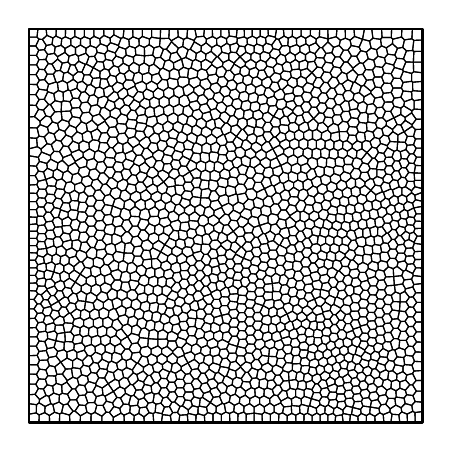
\begin{tikzpicture}[scale=5.0, line join=round]

    % Domain.
    \draw[thick]
        (0,0) -- (1,0) -- (1,1) -- (0,1) -- cycle;
    
    % Cells.
    \foreach \polygon in {
		{(0.52783361130011,0.67461028897455)--(0.53917393412947,0.67119182707563)--(0.54907793809413,0.67784730711481)--(0.55023159096289,0.69016550664769)--(0.53907923704626,0.69960339872957)--(0.52733030611828,0.69702686202945)--(0.52247742171631,0.68915259195291)},
		{(0.94044782484985,0.18996051446578)--(0.92983923563632,0.18371717656422)--(0.93545701072126,0.16669599752454)--(0.95224872022507,0.16486929587327)--(0.95752432650154,0.17076576777647)--(0.95522378217275,0.18457492177474)},
		{(0.19857616993585,0.73623644678544)--(0.20460254827982,0.74901970200764)--(0.19304209038131,0.7653922525548)--(0.17507498633215,0.75391973468047)--(0.17415298980365,0.74592032459422)--(0.18452751058078,0.73520792661)},
		{(0.43761026076379,0.73185012292813)--(0.42832870785124,0.72721359850896)--(0.42477796754536,0.71048964931522)--(0.43943003848359,0.70333015125248)--(0.45124221526515,0.71053384053585)--(0.45079891594922,0.7237516398191)},
		{(0.90228964552821,0.66335159871201)--(0.90869305791256,0.65207493244744)--(0.92196796898942,0.65214133627056)--(0.92941273237938,0.66439355979622)--(0.92255019596676,0.6740064847745)--(0.90680788938203,0.67332609073701)},
		{(0.31492058850294,0.44377577243084)--(0.30726800881538,0.43668325025101)--(0.31173399047684,0.41526354128981)--(0.32619510320582,0.41659980235391)--(0.33490678254499,0.43341551399385)},
		{(0.21042841789723,0.5925562621445)--(0.20572547612573,0.57919241887248)--(0.21864258095483,0.56691264615714)--(0.23054517989198,0.57090790838625)--(0.23506191548599,0.58787975958504)--(0.22393054841557,0.59730892147301)},
		{(0.1853419933766,0.17179350086672)--(0.16929943530352,0.17855014512131)--(0.15803092055081,0.16878393003167)--(0.16422170301741,0.15275834886864)--(0.17560875941163,0.15029170098148)--(0.1862105999475,0.1607612183053)},
		{(0.57305367877739,0.74852514440855)--(0.57685019976343,0.7513643625941)--(0.57796941995566,0.76840584744202)--(0.56931148967265,0.77509982883747)--(0.5540346915435,0.76806311648098)--(0.55525243386983,0.75462329296203)},
		{(1.0,0.13213029237563)--(1.0,0.15419392543976)--(0.97958899898127,0.15525370009625)--(0.97308138966469,0.14560432421604)--(0.97830309900243,0.13059426235672)},
		{(0.61975598516988,0.69510760191998)--(0.60282727765184,0.68522706893216)--(0.60266408988052,0.67354204489123)--(0.61394770222196,0.66556132236288)--(0.62983010318696,0.6727573293968)--(0.63069414520196,0.67525741322725)},
		{(0.91903942669386,0.22867967686734)--(0.90592892725672,0.22828300615704)--(0.90080270897902,0.22204072133185)--(0.90551865848543,0.20564435326456)--(0.91852525130018,0.20443557084815)--(0.92711072609128,0.21319201673992)},
		{(0.55913627135488,0.83331905004684)--(0.55031187331604,0.84116329320131)--(0.53619519135401,0.8370778909435)--(0.53285097678884,0.82301948873815)--(0.54184148664246,0.81445128640262)--(0.55727443857875,0.81795889100812)},
		{(0.90406250547368,0.25114588334222)--(0.91785763936674,0.25265925628308)--(0.92315908774548,0.26212474240369)--(0.91550774675631,0.27568060959173)--(0.9042277544525,0.27594133521002)--(0.89729213439011,0.26678778856744)},
		{(0.92719595434386,0.57647782890812)--(0.92372277328378,0.59060796397152)--(0.91929181129579,0.59313203379209)--(0.9005962909747,0.58490296684439)--(0.90573612278947,0.56976004035684)--(0.91466388710103,0.56659848790501)},
		{(0.71001174304026,0.41874055670722)--(0.71782563131625,0.40523733427791)--(0.72660639334041,0.40511837024525)--(0.73580303621938,0.41608226589769)--(0.73259003712286,0.42823990480563)--(0.72015820462868,0.43122326894014)},
		{(0.29485521269872,0.66087178089592)--(0.28031413370911,0.65146654985957)--(0.28289273305498,0.63713387218138)--(0.2991731338926,0.63195651204632)--(0.30783646309814,0.64727729556916)},
		{(0.63998834224195,0.4904069354838)--(0.62831671241166,0.50434526534404)--(0.61524301148739,0.50152417875459)--(0.6131155509498,0.48613812493526)--(0.62666228016869,0.47666187245115)--(0.63587041371831,0.47960200767144)},
		{(0.37637983341862,0.087877434525916)--(0.37059752423543,0.078112500865848)--(0.3779822965632,0.065830992489997)--(0.39233162294136,0.065834510885811)--(0.39774990116104,0.077375019101063)--(0.39238713262638,0.088239121562696)},
		{(0.17773402465232,0.28428765533896)--(0.18937800285695,0.29157115059575)--(0.18962407290851,0.30458422645039)--(0.17293509993097,0.31380163623905)--(0.1636203771048,0.30353394239176)--(0.16691443128614,0.28861361318455)},
		{(0.72490898225929,0.51046322857639)--(0.7375673021723,0.51976094843243)--(0.73540243506575,0.53271848604501)--(0.72380275690257,0.53712398723007)--(0.71195251743032,0.52826197736461)--(0.71233950327391,0.51736378094751)},
		{(0.7303040444152,0.97395717409101)--(0.72923923193785,0.96451563587777)--(0.73914012743514,0.95244796360016)--(0.74538821179777,0.95183162999074)--(0.75976170160102,0.96656718557574)--(0.76012886679852,0.97428118660798)--(0.73814215908806,0.97972964687632)},
		{(0.079840301373368,0.89420533487157)--(0.085076858171501,0.91281386165006)--(0.073390657954633,0.92291409011651)--(0.058877900024522,0.91028550297679)--(0.068635580997239,0.89291231854124)},
		{(0.17495013821071,0.66074861488232)--(0.1652507146425,0.67056384511195)--(0.14849107897761,0.66559190925607)--(0.14620699089641,0.65047528070597)--(0.1552236827782,0.64127692083849)--(0.1697517807103,0.64455641382858)},
		{(0.65963636178747,0.12734041586169)--(0.64604499851388,0.13186206050555)--(0.63764658714396,0.12077765098031)--(0.64688096846507,0.10536050616516)--(0.66088190815247,0.10643336562321)},
		{(0.78864936393509,0.25961785831356)--(0.79807100925141,0.25993003663021)--(0.80497459919587,0.27416336755879)--(0.79176972286947,0.28552248634061)--(0.77952083694004,0.2736638618256)},
		{(0.8024419877741,0.65549030519559)--(0.82044989614412,0.65510722796003)--(0.82536454284306,0.66980549378007)--(0.8093453712825,0.67876991306109)--(0.79961931701585,0.67044215606715)},
		{(0.48598742102354,0.33413175216819)--(0.50031017856349,0.34385574084331)--(0.49558179164072,0.35725387990448)--(0.48178780045101,0.36015198281239)--(0.47532093528486,0.35412752614483)--(0.47826334800962,0.33752265409307)},
		{(0.54493088751862,0.39206025748755)--(0.55846700543962,0.39161783481343)--(0.56564200120243,0.40135795800191)--(0.56337435582918,0.41043499128302)--(0.54537674941784,0.41719485442798)--(0.53867356045679,0.40341029854537)},
		{(0.60672660776945,0.42990013861925)--(0.6121356063288,0.43751547480714)--(0.60603268379732,0.45483426317655)--(0.59009203467418,0.45246026322032)--(0.58543122247828,0.4453481987023)--(0.59190178325245,0.43003855117374)},
		{(0.95685182135078,0.33923742207726)--(0.95490263666968,0.33299244252738)--(0.96686580576235,0.31822768084039)--(0.97600284796757,0.31907832435291)--(0.98281862238488,0.32928874562781)--(0.97539602248522,0.34435111659356)},
		{(0.87759717606953,0.27930775954335)--(0.86292210431425,0.27987672662408)--(0.85667368900975,0.26823247864501)--(0.86249792583706,0.25726956307783)--(0.87840483086641,0.25870132756966)--(0.88342287020604,0.26666556683711)},
		{(0.97674455723686,0.50095376961688)--(0.96156253000935,0.50243892493146)--(0.95531264119626,0.49498576231509)--(0.9571185152865,0.48578507593713)--(0.96758694032588,0.47988485900614)--(0.97757498363723,0.48338773829389)--(0.98084135743256,0.49249223946991)},
		{(0.69843235409496,0.37104639216394)--(0.69414649574716,0.3611969037555)--(0.70197461641639,0.35003293458883)--(0.71893258610432,0.3522413173806)--(0.72182123118209,0.35793970715523)--(0.7142535866699,0.37439369218974)},
		{(0.56094509373759,0.89628692892025)--(0.57649218136568,0.90219700445491)--(0.57748861627414,0.91330199165323)--(0.56411517274671,0.92232079077964)--(0.55071939373472,0.91403234124589)--(0.54952986191417,0.90662118094132)},
		{(0.6456624026678,0.29203146022003)--(0.65610580970123,0.27585247860674)--(0.66968987065897,0.28248816754046)--(0.67170196108471,0.29533468918193)--(0.66166165593326,0.3039296228739)--(0.64865123439629,0.30026902804045)},
		{(0.42969315122859,0.38607485568471)--(0.42055437229139,0.39961195326783)--(0.40954503464483,0.39813197213335)--(0.40357961314395,0.38601074348822)--(0.4101242172351,0.37429426989052)--(0.42117478085927,0.37385000866678)},
		{(0.25379809921109,0.51541788406673)--(0.25949348579471,0.52369681985896)--(0.25620118705772,0.53839301939306)--(0.24138811225651,0.54456117515296)--(0.23531458055341,0.54108719233366)--(0.23097570604762,0.52450772691243)--(0.24110851972288,0.5136711222114)},
		{(0.28770910573859,0.4001756272894)--(0.27531450797065,0.39600841036881)--(0.27233160686526,0.38393246021516)--(0.28408502561332,0.37198731953304)--(0.29507410069999,0.37477576106929)--(0.2989266183071,0.38992678889917)},
		{(0.1652323475329,1.0)--(0.14108410451052,1.0)--(0.14104091103489,0.9799334906313)--(0.15580636134251,0.97403028799229)--(0.16558050796402,0.98067472758818)},
		{(0.53627674531552,0.92885207616739)--(0.52716426912996,0.93947048549709)--(0.51284206029115,0.94063053460307)--(0.50781500520468,0.93603116589683)--(0.50801558499613,0.92133932392206)--(0.52113793662174,0.91279170390853)},
		{(0.22410222207864,0.31707020449245)--(0.23629903196516,0.30977500176839)--(0.2496945804259,0.31775881599248)--(0.24989102371426,0.32994863078906)--(0.23312990401326,0.33794684966373)--(0.2248077174747,0.33355392330643)},
		{(0.59831470965417,0.73795252113162)--(0.59416477324474,0.72977035914777)--(0.60329926255818,0.71332946351043)--(0.61012140945206,0.71266593356408)--(0.62191263072991,0.72530640849159)--(0.6130477511822,0.73855547530203)},
		{(0.64604499851388,0.13186206050555)--(0.65963636178747,0.12734041586169)--(0.66931277181283,0.13284372573166)--(0.66996776101629,0.14898795624448)--(0.66830637561142,0.15087934215078)--(0.65368220405144,0.15221766442216)--(0.64428567644095,0.13843105803045)},
		{(0.14426479401631,0.30720010822599)--(0.12560836155399,0.30962957288371)--(0.11798636369244,0.30131799609505)--(0.12122778092119,0.28857191401467)--(0.13203984291405,0.2832440247356)--(0.14135312985527,0.28745842433993)},
		{(0.60283972941214,0.12597203746534)--(0.59022080023195,0.13678309483944)--(0.58224139022199,0.13286713976405)--(0.57866871457492,0.11343287463539)--(0.58592802421299,0.10804932547353)--(0.60065584825025,0.11159586264383)},
		{(0.60858804611033,0.45864207529407)--(0.60603268379732,0.45483426317655)--(0.6121356063288,0.43751547480714)--(0.62839825285096,0.43796664605871)--(0.63528936650662,0.44961806736589)--(0.62135721604277,0.46203330651055)},
		{(0.38709992139713,0.5762951441186)--(0.39629635540817,0.58886010701443)--(0.3918058370933,0.6020764174503)--(0.37274292761038,0.60272963719068)--(0.37089131064252,0.60044832653151)--(0.37374428538532,0.58067952947603)},
		{(0.94259273296606,0.087170065427661)--(0.95638815376741,0.081943544621922)--(0.96794936026225,0.095673761188427)--(0.95699631947872,0.10795992376485)--(0.94218385635824,0.10295378210088)},
		{(0.9571185152865,0.48578507593713)--(0.95531264119626,0.49498576231509)--(0.94086002212658,0.49874215653559)--(0.93199142729906,0.48932275855637)--(0.93902569473585,0.47519407823101)--(0.94529651364495,0.47464539764795)},
		{(0.0,0.65225127745982)--(0.0,0.6270056818027)--(0.016064715994848,0.62696037945065)--(0.02451954559738,0.63847606291916)--(0.018997471016997,0.65108354380552)},
		{(0.77884496965697,0.42917729292269)--(0.76493569777416,0.43521496661364)--(0.75739808368679,0.42997791196728)--(0.75620856570572,0.41511578685382)--(0.77338548269824,0.40912033399281)--(0.77916526643003,0.41294336650886)},
		{(0.040411694288055,0.02507796583275)--(0.041481458926964,0.040559951592713)--(0.026318572957658,0.049928340218348)--(0.019613860475396,0.045173882026416)--(0.019048672444417,0.024240035359348)--(0.026254734758618,0.019089855704364)},
		{(0.93088598298124,0.3316416653415)--(0.92061973790219,0.32268571232483)--(0.92550178607467,0.30719931808726)--(0.94306825910008,0.30651689456173)--(0.94314602561234,0.32679459335125)},
		{(0.41932503764378,0.11041159332827)--(0.41241728977536,0.099496401806893)--(0.42009058822933,0.084456298878481)--(0.43436685596597,0.087015675085652)--(0.43943889795397,0.098141321351919)--(0.42890182485464,0.11126949243259)},
		{(0.27041440283542,0.95099387071235)--(0.27184318785361,0.93363549598281)--(0.29405144828679,0.93133649709868)--(0.29366735136304,0.95263771464771)--(0.28052547246738,0.95827467421395)},
		{(0.037800359223152,0.54713152555254)--(0.024383545921923,0.54757741331254)--(0.019251608321978,0.54061218096458)--(0.023204372924869,0.52391845573253)--(0.03708165467032,0.52356806169278)--(0.044836511790612,0.53403536603734)},
		{(0.28031413370911,0.65146654985957)--(0.29485521269872,0.66087178089592)--(0.29581824754139,0.66763683404309)--(0.2858125943412,0.67949218442316)--(0.27354919360959,0.67840297244057)--(0.26554013190155,0.66252684134946)--(0.26740488540637,0.65722945757285)},
		{(0.24745268771788,0.9331791762107)--(0.26579382524067,0.92760657862766)--(0.27184318785361,0.93363549598281)--(0.27041440283542,0.95099387071235)--(0.25563309560784,0.95610619697037)--(0.24585442376937,0.94827555354223)},
		{(0.81684159780243,0.38743493989153)--(0.83464108091559,0.39030189324146)--(0.83710382055899,0.40056750991299)--(0.82356378067447,0.41320103172872)--(0.8173092858951,0.41170967868651)--(0.81075166869462,0.39611655562579)},
		{(0.20997922237426,0.38362250863958)--(0.22717383874383,0.38862593953641)--(0.22855318175604,0.40615030771834)--(0.21644620155248,0.41228170149572)--(0.20166285461502,0.39947493973301)},
		{(0.53285097678884,0.82301948873815)--(0.53619519135401,0.8370778909435)--(0.52603784207469,0.84702603537158)--(0.51273855725794,0.84312285855469)--(0.50868744057623,0.83067624721396)--(0.51934177873678,0.81953779796011)},
		{(0.84817616510234,0.88428207522102)--(0.85569027425962,0.896316758698)--(0.84875291036529,0.91190295358744)--(0.84092351004369,0.91379913548721)--(0.82342678727923,0.90008572613534)--(0.82314536362447,0.89647146314129)--(0.83625806576254,0.8829199766337)},
		{(0.42734931679301,0.76837834059725)--(0.42465602798276,0.7553438601287)--(0.43962302658725,0.74584130903515)--(0.44971457447744,0.75164295956696)--(0.45120610406398,0.76317317976519)--(0.43932909188771,0.7735501191371)},
		{(0.0,0.39280375526495)--(0.0,0.37377611680429)--(0.016926217940501,0.37359938535319)--(0.022863944966988,0.38619397092635)--(0.019964150745797,0.39289255665915)},
		{(0.24276830003952,0.0)--(0.26686180469446,0.0)--(0.26772542152921,0.017286891801228)--(0.25651251669848,0.024979419762638)--(0.24180488315883,0.018540089573588)},
		{(0.0,0.070391462657215)--(0.0,0.047813170972895)--(0.019613860475396,0.045173882026416)--(0.026318572957658,0.049928340218348)--(0.027405531926193,0.058366256857923)--(0.016016910896049,0.071662260501993)},
		{(0.44591952873517,0.017587395266954)--(0.4543700855801,0.025103901716538)--(0.45116121997642,0.038455294305813)--(0.43326911542514,0.041456893615731)--(0.43009825917467,0.039045450704279)--(0.42966342255645,0.022324006827649)},
		{(0.063575676843492,0.38227664893289)--(0.078631456394358,0.37740999060906)--(0.088970289141495,0.38453608250358)--(0.088854153540435,0.3977863024266)--(0.079136531113605,0.40427562033028)--(0.067812973630468,0.40088854683836)},
		{(0.35572503023977,0.47394489418476)--(0.36766855647606,0.48808220482468)--(0.35910128540039,0.50211912593726)--(0.34285621028206,0.49578381128925)--(0.34199778516619,0.48162376590509)},
		{(0.47890501560772,0.66301391160247)--(0.47179713022979,0.65955528503118)--(0.47078300091105,0.64059695960136)--(0.48455041323272,0.63474766547453)--(0.49570270603683,0.64442248736564)--(0.49403883810969,0.65588344102991)},
		{(0.44779266151642,0.54478479844064)--(0.43521179518122,0.55365533779618)--(0.42177305542687,0.54630539692647)--(0.4215855747601,0.53545765352663)--(0.43493861973225,0.52465508772499)--(0.44377636516185,0.52743644406609)},
		{(0.1652507146425,0.67056384511195)--(0.17495013821071,0.66074861488232)--(0.18981403143226,0.66301730664823)--(0.19563376073702,0.67341932801365)--(0.1926193013591,0.68366849064924)--(0.17634286093353,0.69089230799546)--(0.16811993131669,0.6870240856289)},
		{(0.16689126752061,0.44423818726184)--(0.17272544328679,0.43797016086782)--(0.1929364866781,0.44021395744752)--(0.19680649165985,0.45075819184497)--(0.18613167491918,0.46322052416101)--(0.17482351930403,0.46249477096433)},
		{(0.64659937301628,1.0)--(0.62961045671277,1.0)--(0.62575483915519,0.97874796528384)--(0.62859335510869,0.97453854134234)--(0.63465938236772,0.97305417613295)--(0.64842789154515,0.98134543722828)},
		{(0.83924988373766,0.83809523223243)--(0.8516506198057,0.8270861390024)--(0.8685590729463,0.83649754052698)--(0.86910616541782,0.84140312725638)--(0.85133539643343,0.85646573625244)--(0.84452822354764,0.85413955573924)},
		{(0.37285355621947,0.35587777274683)--(0.3812503259559,0.35522146291345)--(0.38950525227976,0.36415480067667)--(0.38341962098136,0.38170709092329)--(0.36874484863596,0.37981025613221)--(0.36408659025406,0.3674594805606)},
		{(0.67195427416074,0.16927805052149)--(0.68590319235166,0.17083665838363)--(0.69006800189245,0.18434602440559)--(0.68540790797193,0.19184068453061)--(0.66965427635987,0.1907280021267)--(0.66561931303306,0.17563592634345)},
		{(0.25783791557769,0.096943527708853)--(0.26458188999658,0.095442093873286)--(0.27799406446907,0.10761200321943)--(0.27431652002578,0.12163155091765)--(0.26558866920838,0.12603980214482)--(0.25075161002121,0.11161376620381)},
		{(0.97642768029057,0.29280070821811)--(0.96569927579088,0.29347359139447)--(0.95649301464563,0.28152999013406)--(0.96330754739765,0.26856556038112)--(0.97617910821123,0.26826237870463)--(0.98399663778145,0.28011323449465)},
		{(0.46975751129214,0.2269611561919)--(0.46929104569719,0.21375723775788)--(0.48042654112633,0.20503400242634)--(0.49164000338243,0.21088861304206)--(0.49295789988638,0.22730446738119)--(0.48539568882127,0.23327409912186)},
		{(0.25949348579471,0.52369681985896)--(0.25379809921109,0.51541788406673)--(0.26353590604303,0.4988295561559)--(0.27630257492041,0.49889304002461)--(0.28387570280079,0.51700828344728)--(0.28037734250045,0.52266126432927)},
		{(0.25077541959804,0.71241325770075)--(0.25335726821488,0.72124464725127)--(0.24385870268605,0.73478464948452)--(0.22879685859613,0.73336213022549)--(0.22277961786772,0.72433367288261)--(0.22728368599327,0.71120546470079)--(0.23898722363344,0.70644333264177)},
		{(0.55129068231307,0.32234111517532)--(0.55688135190252,0.33287774517954)--(0.55232088328945,0.34373719652779)--(0.54175244925683,0.34651592473417)--(0.53156494405461,0.3387221772414)--(0.53052285438136,0.32722162166989)--(0.53331020204381,0.32340966817131)},
		{(0.085918141501947,0.86843628441201)--(0.097670914014562,0.86207560342134)--(0.11295129309515,0.87148684573944)--(0.11260426229461,0.88049877526382)--(0.099003632996196,0.88978143580032)--(0.088855805537031,0.8873935017615)},
		{(0.83001735650257,0.59965733608246)--(0.81819176059873,0.59326306925153)--(0.82031575187655,0.57677202001989)--(0.83358573211878,0.57284000438424)--(0.84237187524479,0.58011577573455)--(0.84090418036082,0.59430926477534)},
		{(0.53470507349304,0.2555834683465)--(0.52785580009627,0.26490156322705)--(0.51549443678179,0.26447518478992)--(0.50772255028899,0.25029216496498)--(0.5120063220833,0.24229642068994)--(0.52899093398864,0.24194603425407)},
		{(0.081622709865678,0.7144319573877)--(0.087841271614734,0.70245065668888)--(0.10036316881876,0.70073833675735)--(0.1118562278146,0.71467787090959)--(0.10900537392811,0.72443372751205)--(0.094486330086326,0.7303059510609)},
		{(0.94145047088217,0.28314856821539)--(0.93735738523273,0.26372136117196)--(0.94459943245563,0.25639163738677)--(0.95558999483026,0.25697780195296)--(0.96330754739765,0.26856556038112)--(0.95649301464563,0.28152999013406)},
		{(0.16345236243205,0.57610062635294)--(0.17194307617017,0.56399879014774)--(0.18790398423748,0.56439279929984)--(0.19363619588546,0.57581248641707)--(0.18099241121089,0.59126477195995)--(0.16952516578545,0.58876456687338)},
		{(0.24180488315883,0.018540089573588)--(0.25651251669848,0.024979419762638)--(0.25777213836351,0.041692986621427)--(0.25375666387262,0.045784465463533)--(0.24056383936023,0.046634579526196)--(0.23110389769436,0.035887030069277)--(0.2340709755005,0.023643571436711)},
		{(0.43308892126226,0.59698449797451)--(0.43869573774093,0.61623814626365)--(0.43481188876842,0.62135671150761)--(0.41853415476601,0.62047583006324)--(0.41244443296135,0.61020120200373)--(0.41974711566476,0.59649266427987)},
		{(0.3978355259484,0.098986466696529)--(0.41241728977536,0.099496401806893)--(0.41932503764378,0.11041159332827)--(0.40907826802239,0.12443969329672)--(0.39829491531386,0.12235446640221)--(0.39213093858448,0.10929566998076)},
		{(0.82044989614412,0.65510722796003)--(0.8024419877741,0.65549030519559)--(0.79771162050527,0.64939766095723)--(0.80001983523935,0.63708150187897)--(0.81638505414589,0.63162338826874)--(0.82619805065443,0.64559110765445)},
		{(0.19304209038131,0.7653922525548)--(0.20460254827982,0.74901970200764)--(0.22046101041012,0.75139226925296)--(0.22557679608584,0.75961043177193)--(0.22284530716778,0.77081735428536)--(0.2068498962834,0.77790721075025)--(0.19352793459018,0.76803666720661)},
		{(0.91758332808507,0.71373997153119)--(0.91032613714898,0.70325107106938)--(0.91153517233354,0.6980906389802)--(0.92772996984358,0.68882667026648)--(0.93540900605583,0.69183296352199)--(0.93697732278915,0.71260113202551)},
		{(0.0,0.21739507456111)--(0.0,0.19400165171829)--(0.018884186519577,0.19388643558657)--(0.026496288866262,0.20674079440548)--(0.020562613522291,0.2176746036379)},
		{(0.18937800285695,0.29157115059575)--(0.17773402465232,0.28428765533896)--(0.17954383047188,0.26727217488205)--(0.18786701123854,0.26234532216733)--(0.2016455492445,0.26802641439067)--(0.20367612237942,0.28350495077019)},
		{(0.92401467035876,0.74434717636676)--(0.9246341761055,0.7386902370581)--(0.93770300334222,0.73042462829374)--(0.95329505792465,0.73837486521044)--(0.94497368579436,0.75550983992482)--(0.9354166805156,0.75700451023475)},
		{(0.62338851098712,0.026357093996815)--(0.62311526652138,0.042032235347816)--(0.61255807609753,0.048952290017295)--(0.59806577513912,0.039752763755206)--(0.59883436658345,0.026155909312692)--(0.61368986277221,0.020742378541545)},
		{(0.62839825285096,0.43796664605871)--(0.6121356063288,0.43751547480714)--(0.60672660776945,0.42990013861925)--(0.61219332668415,0.41544097405086)--(0.62694471320573,0.41457043275189)--(0.63421590167146,0.42429494755678)},
		{(0.62815880113976,0.16715239815295)--(0.60956150576582,0.16797277071616)--(0.60759955975335,0.15151207475692)--(0.61973650790729,0.14192595401466)--(0.62830380049165,0.14619018717298)--(0.63183726174843,0.16257903842536)},
		{(0.67284283241575,0.69354108842018)--(0.67264795418739,0.6797931899192)--(0.68290904263596,0.67245125029031)--(0.6961322446819,0.67887688521438)--(0.697690589493,0.69301312627131)--(0.68598967793869,0.7001084355866)},
		{(0.86068396661918,0.63557323234151)--(0.86705479535722,0.61961227845748)--(0.87444914695997,0.61776079576974)--(0.88417737183965,0.62493364047651)--(0.88431958178246,0.64239491429559)--(0.8829843838194,0.64389975965922)--(0.86699569864859,0.64495436650423)},
		{(1.0,0.051554378674108)--(1.0,0.079673606141589)--(0.98456475838885,0.07961274587156)--(0.97570567295498,0.068383441425921)--(0.98138207335056,0.053157841531733)},
		{(0.1982538992406,0.23912193130823)--(0.19717254837209,0.22271322190809)--(0.20750162386324,0.21529941200047)--(0.22060595360721,0.22117880169807)--(0.22374272879992,0.2328391288196)--(0.2101996614196,0.24382147630886)},
		{(0.055666815459189,0.66878715230213)--(0.04556494324729,0.65800732102792)--(0.047322421171774,0.64560753133116)--(0.062888532712909,0.63876394812733)--(0.071722820635382,0.64398004867496)--(0.073984288029498,0.65915036154064)},
		{(0.87241336450365,0.4474810286701)--(0.85623393275352,0.45115373222266)--(0.85013103501825,0.44594309102163)--(0.85260531869516,0.42751287387848)--(0.86932234586408,0.42552759959214)--(0.87372329203179,0.42981504657047)},
		{(0.73240821208449,0.66801300406206)--(0.71905410047592,0.67325379517659)--(0.7099174241794,0.66871644792274)--(0.70726915635242,0.65838779238824)--(0.71715050125116,0.64455529820481)--(0.72472036467258,0.6436870675037)--(0.7338478748518,0.65131583025274)},
		{(0.091977767135845,0.94001884358126)--(0.10222266043808,0.93032103288703)--(0.11882487056881,0.93573593962977)--(0.11863924842393,0.95163997661129)--(0.10709302044387,0.95838020391055)--(0.092083280515782,0.95006796224089)},
		{(0.44082141497199,0.064086063014124)--(0.46096876900313,0.05061749486646)--(0.46861718503632,0.063842548698931)--(0.4598134634223,0.078984526318236)--(0.4441365373708,0.073917087311968)},
		{(0.63528936650662,0.44961806736589)--(0.62839825285096,0.43796664605871)--(0.63421590167146,0.42429494755678)--(0.64907585343684,0.42303395687276)--(0.65576816249703,0.43103566012819)--(0.65437514638168,0.44200603519737)--(0.637840600799,0.45032472562722)},
		{(0.24722106015569,0.87025902792156)--(0.23894774291236,0.85956897746862)--(0.24131692519801,0.85017247116173)--(0.24958869652613,0.84483815977839)--(0.26936005596758,0.85440779911586)--(0.27043010656677,0.85983373046755)--(0.26365366313701,0.86917249822077)},
		{(0.72373570344293,0.19971203001186)--(0.71135914100009,0.19559333803948)--(0.70837347269905,0.18380238889264)--(0.71026970775724,0.18043818214025)--(0.72612574116498,0.17647741551884)--(0.7339578106525,0.18334152740347)--(0.73324920424651,0.19294596396336)},
		{(0.55688135190252,0.33287774517954)--(0.55129068231307,0.32234111517532)--(0.55530476008451,0.31296899611713)--(0.57324678325616,0.31050297455475)--(0.57865290327807,0.32022536352973)--(0.57354510223557,0.33221826892327)},
		{(0.25081315726106,0.2182554830696)--(0.23428386397232,0.20799112941262)--(0.23266928204135,0.20069821956034)--(0.24478369661438,0.1863543614811)--(0.25465885729046,0.18687486209816)--(0.26169585604108,0.20004934981731)},
		{(0.74964892472551,0.86415958024919)--(0.73832173149418,0.8490728785552)--(0.74399763976844,0.83797571422365)--(0.75504264522624,0.83593743279709)--(0.76705276305184,0.84991391238464)--(0.75913017755385,0.86296992957744)},
		{(0.34539714187186,0.45179247514388)--(0.36374954886424,0.44078997679853)--(0.37314890165235,0.44794285121347)--(0.37359934921862,0.46090821317515)--(0.35707522769494,0.46834788088421)},
		{(0.57005476242789,0.22239835779643)--(0.57620145245991,0.23391937001677)--(0.56796478419284,0.2453858093239)--(0.55556441392045,0.24475837517424)--(0.54925836127735,0.2330930689518)--(0.55580510558584,0.22121395185112)},
		{(0.079505853925992,0.54264948213408)--(0.080796908577753,0.54016159773096)--(0.09986982738355,0.53368871554934)--(0.10667758774106,0.54049202953362)--(0.10275803024641,0.55723091315258)--(0.087372969164545,0.55846374541074)},
		{(0.25374798529844,0.26622232604671)--(0.2673852047749,0.27001322729389)--(0.27033415109751,0.28563009027379)--(0.25940624024491,0.29378005401802)--(0.24741950832671,0.28935751812403)--(0.2451019679105,0.27367345736154)},
		{(0.77875182736829,0.31650626823199)--(0.78277488613045,0.31850020542169)--(0.78733024530301,0.33424397416132)--(0.77929138467388,0.34364476785098)--(0.76939564585793,0.34298784413886)--(0.76196419332226,0.33287140153971)--(0.76376901313671,0.32305836483369)},
		{(0.90310690066879,0.64169224363739)--(0.88431958178246,0.64239491429559)--(0.88417737183965,0.62493364047651)--(0.89902494828695,0.61976118090944)--(0.90760095363987,0.63117862607177)},
		{(0.80001983523935,0.63708150187897)--(0.79771162050527,0.64939766095723)--(0.77941855725496,0.65231906596313)--(0.77366021805888,0.64661080984267)--(0.77512745310741,0.63239598327983)--(0.79066591848278,0.62682491802056)},
		{(0.28088416101612,0.90665089845696)--(0.2796214327662,0.88998265185149)--(0.28870557050555,0.88381293390677)--(0.30417400622606,0.88882272683041)--(0.30597147752698,0.90525014471683)--(0.29303293647216,0.91338359673149)},
		{(0.59416477324474,0.72977035914777)--(0.59831470965417,0.73795252113162)--(0.59342136462412,0.74798671458533)--(0.57685019976343,0.7513643625941)--(0.57305367877739,0.74852514440855)--(0.57102613383062,0.73377250039468)--(0.57955088664928,0.72588975862049)},
		{(0.97665033635264,0.21871175946304)--(0.96529910840349,0.21845027374574)--(0.95866812044376,0.20847650772357)--(0.9647485573168,0.19418247318713)--(0.97582845911127,0.19275456655202)--(0.98522287393573,0.20445275405262)},
		{(0.16929943530352,0.17855014512131)--(0.1853419933766,0.17179350086672)--(0.19442375421816,0.17981764024345)--(0.19349056021994,0.19451690559646)--(0.18323977754428,0.20027559141091)--(0.16807904267423,0.19236103396293)},
		{(0.068635580997239,0.89291231854124)--(0.058877900024522,0.91028550297679)--(0.049569084767122,0.91161367024722)--(0.039598665094208,0.89625481443988)--(0.046900795022988,0.88460539155669)--(0.062411826641681,0.8849540807689)},
		{(0.37874458671398,0.64210431870413)--(0.38337907116513,0.62817218371799)--(0.39179716016607,0.62526913326752)--(0.40890151068044,0.63684448837187)--(0.40011087081404,0.65047805833735)--(0.38685382214166,0.65184607155358)},
		{(0.22597052924267,0.61002976902403)--(0.23985819671197,0.61773447171281)--(0.234242634843,0.63617411967554)--(0.22009634984944,0.63700049063617)--(0.21176285558147,0.62192629437585)},
		{(0.81493070724338,1.3552527156069e-20)--(0.83668047710381,1.3552527156069e-20)--(0.83589322497074,0.015121663327101)--(0.81962002632565,0.020837608234082)--(0.81695374788695,0.018998904493874)},
		{(0.48608561353458,0.18517549177424)--(0.47906866310618,0.19335764703994)--(0.46155177229874,0.18798201602104)--(0.46049194536925,0.17264177599764)--(0.46727102549336,0.16748540789255)--(0.48286713062014,0.17182465083516)},
		{(0.44720136343333,0.0)--(0.46800335262624,0.0)--(0.46781346133908,0.021392155641481)--(0.4543700855801,0.025103901716538)--(0.44591952873517,0.017587395266954)},
		{(0.4215855747601,0.53545765352663)--(0.42177305542687,0.54630539692647)--(0.41041196764121,0.553883550035)--(0.39556732604359,0.54371324789372)--(0.39527950555696,0.53393795614961)--(0.40687125618084,0.5256753258946)},
		{(0.56158597220555,0.65087889312922)--(0.57188927496979,0.64684953434466)--(0.58761303282889,0.6577411067735)--(0.58808110387011,0.66479394979242)--(0.57550459376879,0.67591189014299)--(0.56340704367932,0.66980172575717)},
		{(0.81719108123686,0.32155165352993)--(0.82546814245821,0.32799027556582)--(0.82554335488378,0.34351269705773)--(0.81831814540036,0.34944998305544)--(0.80687767536279,0.34739490596063)--(0.80160424606594,0.33617017174072)--(0.80980311202715,0.32273671378767)},
		{(0.0,0.74888304366753)--(0.0,0.72319286875187)--(0.019782937322629,0.72170092926141)--(0.02606681584901,0.72707830954743)--(0.021152784496093,0.74808071678088)},
		{(0.97872147239783,0.81735358427001)--(0.97332157390183,0.82163244534978)--(0.95434932871825,0.81473972023033)--(0.95241855179269,0.80423847789188)--(0.97337267622862,0.79157578540264)--(0.97871493680427,0.79618346743027)},
		{(0.318694330143,0.23653398000054)--(0.32825166897848,0.23019627290322)--(0.34133748029152,0.2358870856573)--(0.34295610609848,0.24936807358206)--(0.33269719941952,0.25748622490388)--(0.3206608644571,0.2541995611311)},
		{(0.71183721931977,0.95652609375487)--(0.70402786569059,0.96176283396403)--(0.68818783261255,0.95419123338435)--(0.6888940291103,0.94152871920237)--(0.70276432343788,0.93385829082746)--(0.71362428653974,0.94179364500152)},
		{(1.0,0.63312808516349)--(1.0,0.65240105047129)--(0.9823227661363,0.65272842376861)--(0.97880394182912,0.63387700924393)},
		{(0.14937727299449,0.17047754362061)--(0.14108722946059,0.18371678384318)--(0.122337945311,0.17752929653475)--(0.1220724061208,0.16354953752547)--(0.13613905492575,0.15655858226193)},
		{(0.81035307013564,0.19044805546222)--(0.81173862880739,0.17726987974028)--(0.82471294351271,0.17136874411323)--(0.82895413511593,0.17332723426904)--(0.83344140908527,0.19164334942811)--(0.82124355452132,0.19775786820867)},
		{(0.090301451548297,0.20334590489019)--(0.068722056732382,0.20753328795323)--(0.064241132725413,0.19111394503908)--(0.07338110545457,0.18054557784655)--(0.089264795917984,0.18481453038416)},
		{(0.83683407671795,0.30374657081552)--(0.84398566545402,0.31375421071706)--(0.84066923644454,0.32353875158996)--(0.82546814245821,0.32799027556582)--(0.81719108123686,0.32155165352993)--(0.82285319046965,0.30497833840354)},
		{(0.82619805065443,0.64559110765445)--(0.81638505414589,0.63162338826874)--(0.81911210646068,0.62205437760793)--(0.82960613121436,0.61695038995583)--(0.84010006026992,0.62150505937491)--(0.84428065183071,0.63499044291239)--(0.83810743270824,0.64421777335962)},
		{(0.30591150734654,0.28470714979271)--(0.31457912307281,0.27844564867238)--(0.3265881329512,0.28149476179376)--(0.32988287790265,0.30069415638998)--(0.32524689817079,0.3052000512863)--(0.30767804424852,0.30183120007299)},
		{(0.8376497574559,0.81014671531587)--(0.82347716125648,0.82107972166995)--(0.81220364388061,0.81504821708757)--(0.81628364437745,0.79389711353318)--(0.83390757840572,0.79686318061557)},
		{(0.32825166897848,0.23019627290322)--(0.318694330143,0.23653398000054)--(0.30601502953555,0.2324779235446)--(0.30381347632877,0.21301992227898)--(0.32759942534944,0.21103566314674)},
		{(0.31736843577012,0.91026766110658)--(0.30597147752698,0.90525014471683)--(0.30417400622606,0.88882272683041)--(0.31258688958658,0.88185830977604)--(0.32995508148017,0.88705363814764)--(0.333949014496,0.89688882890591)},
		{(0.93051592959743,0.14673269952666)--(0.92416455882215,0.13153943226836)--(0.93515364659133,0.1222994769118)--(0.95042674853221,0.12924185151239)--(0.95069702626457,0.1427432369468)},
		{(0.26579382524067,0.92760657862766)--(0.24745268771788,0.9331791762107)--(0.23850875021305,0.924721947398)--(0.23990278179638,0.91273106059075)--(0.25430719380502,0.9049886842504)--(0.26649566317463,0.91469030834106)},
		{(0.84152424090927,0.24258026569364)--(0.82430417922061,0.23700783240266)--(0.82298618042626,0.23375345240347)--(0.83036578419128,0.21800713211925)--(0.83904396401469,0.21666385048225)--(0.8475301614608,0.22739104957602)},
		{(0.71135914100009,0.19559333803948)--(0.72373570344293,0.19971203001186)--(0.72564208571365,0.2154861782971)--(0.72260892737945,0.21889189460911)--(0.70616644055638,0.21705720081099)--(0.70289824972592,0.20520908972489)},
		{(0.48397258683245,0.40136740543351)--(0.47750844522284,0.41739913252484)--(0.46344299068745,0.41606878507765)--(0.45699492091706,0.40044119777143)--(0.46484033772249,0.39357082510419)--(0.48196805736453,0.39783597535017)},
		{(0.1338757841631,0.45707111534052)--(0.12925701944006,0.43766041652915)--(0.14560616302888,0.43096836283409)--(0.15716901006357,0.44444080301514)--(0.14677554216067,0.45858551399674)},
		{(0.037974626998962,0.29026328613096)--(0.034469702751271,0.27856566486391)--(0.041468379115865,0.27060889589516)--(0.053545791006014,0.27175807053105)--(0.060136674519943,0.28594542295801)--(0.055561532811545,0.29473123432944)},
		{(0.64118010064861,0.87348178069691)--(0.6566231657946,0.86742380790443)--(0.66680929512032,0.87732707517034)--(0.6643638203809,0.89058441517064)--(0.64654329627252,0.89295432154093)--(0.63893891940708,0.88441525868072)},
		{(0.49842268920583,0.76016460544076)--(0.48405663283085,0.77380565820743)--(0.47154690589476,0.76846545110591)--(0.47459949287665,0.74968146255816)--(0.48763305498683,0.74665644209984)},
		{(0.09089604097493,0.31899460126538)--(0.075575179240841,0.30800099402787)--(0.083847934286155,0.29369066227928)--(0.094458940692178,0.29245346650568)--(0.10417827302493,0.30426853560484)--(0.09906210947121,0.31673364292792)},
		{(0.073390657954633,0.92291409011651)--(0.085076858171501,0.91281386165006)--(0.099626727976002,0.91532068841762)--(0.10222266043808,0.93032103288703)--(0.091977767135845,0.94001884358126)--(0.073133454404277,0.92931167780748)},
		{(0.93791532567721,0.40700181112731)--(0.93539814492961,0.39646925222472)--(0.95140910245183,0.38424609080076)--(0.95740563805684,0.38721826763696)--(0.9617472398295,0.40169286292529)--(0.95499194128149,0.41044617538522)},
		{(0.20460254827982,0.74901970200764)--(0.19857616993585,0.73623644678544)--(0.20575607203387,0.72511751444231)--(0.22277961786772,0.72433367288261)--(0.22879685859613,0.73336213022549)--(0.22046101041012,0.75139226925296)},
		{(0.21864258095483,0.56691264615714)--(0.20572547612573,0.57919241887248)--(0.19363619588546,0.57581248641707)--(0.18790398423748,0.56439279929984)--(0.19331886800443,0.5535728143797)--(0.21292309652953,0.5500915014331)},
		{(1.0,0.51059038047092)--(1.0,0.52975253357502)--(0.98408833960139,0.52973471292593)--(0.97832076416823,0.5205362507417)--(0.9821086488086,0.51164941326592)},
		{(0.45636263687558,0.88159474485373)--(0.4507436947122,0.89420634366517)--(0.43861426803563,0.8982816502677)--(0.42926039837863,0.89231784763375)--(0.4277955064304,0.87735776275572)--(0.43629994551989,0.86862385389535)--(0.45335717560753,0.87403380180133)},
		{(0.64809670071658,0.69277146535877)--(0.662882692614,0.70020963918328)--(0.6622647052171,0.71402063695791)--(0.65340452406458,0.71936791100038)--(0.63803429982431,0.71140624747754)--(0.63676226789014,0.70424244840002)},
		{(0.82357763716381,0.51285325682956)--(0.81500760391381,0.5066668399317)--(0.81667066635593,0.48911329522472)--(0.82681404313399,0.48659692514444)--(0.83818455405216,0.49435762308665)--(0.83570294483999,0.50896480840162)},
		{(0.94160517762935,0.53252176011031)--(0.93200487155373,0.53615265850699)--(0.92054046970311,0.52720411889722)--(0.92405759217136,0.51383999756687)--(0.93776977210875,0.51129223065905)--(0.9448504442998,0.51866553423818)},
		{(0.71782563131625,0.40523733427791)--(0.71001174304026,0.41874055670722)--(0.69940321825653,0.41982890533559)--(0.69013184337218,0.40806839199768)--(0.69588382258535,0.39532737924587)--(0.71012548235064,0.39500327340667)},
		{(0.92536021498882,0.84940051356562)--(0.9463093286884,0.8497476889296)--(0.95080129176906,0.86370797567323)--(0.9438614038758,0.87416274692902)--(0.92654844881615,0.87423891271171)--(0.91966877160577,0.86108426522595)},
		{(0.89329478003203,0.97318315278962)--(0.89594439038134,0.95670258568539)--(0.90803304508443,0.95156663979187)--(0.92381197247179,0.96218088300424)--(0.92435945907448,0.97349271271977)--(0.92073724583988,0.97769551496641)--(0.8973437815039,0.97782177545438)},
		{(0.17194307617017,0.56399879014774)--(0.16345236243205,0.57610062635294)--(0.15074609396583,0.57443633586002)--(0.14410204093866,0.55907843015827)--(0.1508817652476,0.54965067442935)--(0.16457087313824,0.5493996028513)},
		{(0.86705479535722,0.61961227845748)--(0.86068396661918,0.63557323234151)--(0.84428065183071,0.63499044291239)--(0.84010006026992,0.62150505937491)--(0.85423100258896,0.61064440092191)},
		{(0.29405144828679,0.93133649709868)--(0.29303293647216,0.91338359673149)--(0.30597147752698,0.90525014471683)--(0.31736843577012,0.91026766110658)--(0.32174671929348,0.9256446695685)--(0.31466023763844,0.93306242797291)},
		{(0.97510869899334,0.37847650765901)--(0.95740563805684,0.38721826763696)--(0.95140910245183,0.38424609080076)--(0.94739094625828,0.3730286848273)--(0.95346992100378,0.36219295716581)--(0.97229393546675,0.36412382697973)--(0.97657300367392,0.37328608355298)},
		{(0.85569027425962,0.896316758698)--(0.84817616510234,0.88428207522102)--(0.85810155231709,0.86942354385133)--(0.87364410228894,0.87104962084289)--(0.87855967017358,0.87753600546698)--(0.87292702808199,0.89547748173855)},
		{(0.78062861730071,0.07653746058461)--(0.78363539614619,0.072198751956915)--(0.80052334349585,0.072435191484526)--(0.80480691005521,0.080740204131027)--(0.79787616554574,0.093898987413672)--(0.78426342812594,0.09185317907853)},
		{(0.63425628344571,0.0)--(0.65606263729038,0.0)--(0.65664231150785,0.01719477196561)--(0.64447147464413,0.024614176703333)--(0.63525293254667,0.02068088038933)},
		{(0.62983010318696,0.6727573293968)--(0.61394770222196,0.66556132236288)--(0.61292856933278,0.64924550046032)--(0.61920764921812,0.64462321747792)--(0.64024498508344,0.6529368018752)},
		{(0.50232641126804,0.11827266714216)--(0.4968758351701,0.11616390417196)--(0.49151178404448,0.1021492773557)--(0.50421747556063,0.091000065361968)--(0.51653585979002,0.095814362807436)--(0.51830341168567,0.10895122191875)},
		{(0.5377829111883,0.14292843860036)--(0.5510809272927,0.15410719642567)--(0.54720984017904,0.16886390302929)--(0.53015971018626,0.16942998437227)--(0.52577445956705,0.15545010583111)},
		{(0.81831814540036,0.34944998305544)--(0.82554335488378,0.34351269705773)--(0.84151435947173,0.34780096374228)--(0.84446210985842,0.35677700194741)--(0.83543331920653,0.36815624121273)--(0.82250421901252,0.36583740385164)},
		{(0.68572295902382,0.74372243362401)--(0.68570423673841,0.75407555566603)--(0.67621954476818,0.76220729525836)--(0.66348685451967,0.76048807224389)--(0.65920589371028,0.75447674468573)--(0.66136629448589,0.74143285628758)--(0.67459406535142,0.73608904272329)},
		{(0.86256558557964,0.39119830007879)--(0.85515234458653,0.38145055223649)--(0.86222557984183,0.36534215138398)--(0.87966653022357,0.37087606264774)--(0.88178863669503,0.3834962660502)},
		{(0.16218455965644,0.77767741981486)--(0.15358939678199,0.7879469984957)--(0.13668265702183,0.78643972303761)--(0.12985929998044,0.7735812029239)--(0.13337982049059,0.76390300769112)--(0.14583406391625,0.75868826198174)--(0.16060641790858,0.7678590484567)},
		{(0.22367693757231,0.063830948159637)--(0.23293018229228,0.062290566654713)--(0.24578620265843,0.073979252458753)--(0.24375318583896,0.084837057775553)--(0.2313321672734,0.090880691354958)--(0.21508041157697,0.07898469987265)},
		{(0.76508781367607,0.36746571992397)--(0.7765020684744,0.36875671981298)--(0.78484306144131,0.38425038748737)--(0.77116658466722,0.39358073255147)--(0.75982268488705,0.38883673883204)--(0.7575898758221,0.37657227001614)},
		{(0.63895001486955,0.61033840210261)--(0.63499908400068,0.62488640775905)--(0.62136986123904,0.62923409790659)--(0.61196843986523,0.62107952592196)--(0.61702706279161,0.60288239172685)--(0.6226652260201,0.60062428872795)},
		{(0.0,0.90847560906504)--(0.0,0.88345230748486)--(0.018346073131942,0.88372960902266)--(0.02634971270122,0.89705651051393)--(0.01970471977942,0.90841166044153)},
		{(0.52716426912996,0.93947048549709)--(0.53627674531552,0.92885207616739)--(0.55159443699652,0.9404075011157)--(0.54865099173626,0.95448561127362)--(0.53452890632445,0.95622690035663)},
		{(0.31173399047684,0.41526354128981)--(0.30726800881538,0.43668325025101)--(0.29138088069991,0.43806780593)--(0.28436040197068,0.42273332248881)--(0.29144500412616,0.41296676003671)},
		{(0.85931723682177,0.08477129626868)--(0.86275283948418,0.095824769504704)--(0.8532382484462,0.10627266159382)--(0.8418655413029,0.10364998863586)--(0.83764426585462,0.093517450361192)--(0.84493202556386,0.082067723210554)},
		{(0.48366599240683,0.51638059522708)--(0.49821283577496,0.52945348762952)--(0.48956602372941,0.54645956580772)--(0.47082172524467,0.53801669725171)--(0.46978734203973,0.52731029632983)},
		{(0.12296172128307,0.11140369411455)--(0.12739273268199,0.095766525009804)--(0.14196050027359,0.09354963991837)--(0.15171426126106,0.10422956487063)--(0.14868789514064,0.11712674752323)--(0.13426028127129,0.12121360949267)},
		{(0.1697517807103,0.64455641382858)--(0.1552236827782,0.64127692083849)--(0.15164042784535,0.62688375421576)--(0.16276423977019,0.61528575415745)--(0.174607593509,0.61812633286803)--(0.18140763564378,0.63287274974187)},
		{(0.19858510491842,0.71024179039905)--(0.20560434509582,0.69879124618879)--(0.21319704194379,0.6974688127379)--(0.22728368599327,0.71120546470079)--(0.22277961786772,0.72433367288261)--(0.20575607203387,0.72511751444231)},
		{(0.79616002330713,0.019376492034549)--(0.79889244455458,0.02288662673223)--(0.79774528087742,0.031409134700858)--(0.78257553899029,0.039464468766283)--(0.77512060648086,0.03508188850927)--(0.77311961039665,0.022991511103095)--(0.77942663933859,0.01687927214283)},
		{(0.062139103930814,0.46536367196181)--(0.068406094621086,0.47174991644563)--(0.061707811600929,0.48871286021128)--(0.046606543916491,0.48760394461975)--(0.041692822368405,0.47943721526811)--(0.045727023648024,0.46743992009967)},
		{(0.77832537494513,0.9283560250018)--(0.76965913418903,0.93929958622994)--(0.7548684275339,0.93743376181011)--(0.74887608867874,0.92575690882554)--(0.75380133391409,0.91526429581587)--(0.76998441737518,0.91262194201311)},
		{(0.83917682254546,0.95339058555772)--(0.84325011332506,0.94433856962287)--(0.85742404221241,0.94084277532218)--(0.86940218872218,0.95105267171663)--(0.86563976630017,0.96869418136493)--(0.84773079479697,0.973383388416)},
		{(0.71905294578213,0.083578059105033)--(0.72775225726997,0.098233433102401)--(0.71918882521175,0.10710408798972)--(0.70416365257549,0.10179439620473)--(0.7049770705773,0.086606543595455)},
		{(0.0,0.50257956507447)--(0.0,0.48593935666818)--(0.020927214944234,0.48556900370506)--(0.024083318718065,0.49990197243475)--(0.020003563043137,0.50445933470685)},
		{(0.48655790778044,0.62220235807728)--(0.47851293154129,0.61278699876761)--(0.48202125762587,0.60031980025437)--(0.50001217009002,0.59637383067441)--(0.50595759730788,0.6017685173808)--(0.50500314805562,0.61746046043856)},
		{(0.12179638524717,0.51634525741207)--(0.13089594488398,0.50841510556765)--(0.14293103616575,0.50957795956065)--(0.14993777313402,0.52395653131044)--(0.14326212791678,0.53420990184611)--(0.12628830899443,0.53518736453301)},
		{(0.57188927496979,0.64684953434466)--(0.56158597220555,0.65087889312922)--(0.55716619518616,0.64903493981749)--(0.55019832968966,0.62955307071056)--(0.55675093172075,0.62111101819375)--(0.56789367056442,0.62019784459512)--(0.5769477078174,0.63352856905433)},
		{(0.52270723462104,0.88233920400766)--(0.51168093256254,0.89452379349855)--(0.5024556562507,0.89353097085758)--(0.49561342419945,0.87878422205692)--(0.50610980253838,0.86708550861099)--(0.51890492121033,0.87056731509332)},
		{(0.078631456394358,0.37740999060906)--(0.063575676843492,0.38227664893289)--(0.056958378585635,0.36444861938877)--(0.066789072732188,0.35406395398944)--(0.08098434498971,0.36057211040529)},
		{(1.0,0.54906269906636)--(1.0,0.56180815511061)--(0.98216210027125,0.56578038923453)--(0.97480368204762,0.55698414871918)--(0.97778021923975,0.54496515611715)},
		{(0.88217651686928,0.078339145323204)--(0.8897369034949,0.067470122701316)--(0.90628431183752,0.070648106156086)--(0.90954242330344,0.082347487182135)--(0.89713967384281,0.092904184097261)--(0.88558149288202,0.089151052287936)},
		{(0.61255807609753,0.048952290017295)--(0.62311526652138,0.042032235347816)--(0.63978384126044,0.04964853522353)--(0.64058211237257,0.054237765364519)--(0.63189248143333,0.068126778797242)--(0.62289174371396,0.070061264129606)--(0.61175881132291,0.060313392667963)},
		{(0.70658103523528,0.86325746397495)--(0.69534202144684,0.85095331559155)--(0.69893205480459,0.83981808094537)--(0.71562081145527,0.83721470188526)--(0.72451678557517,0.85228025448185)--(0.72134141488214,0.85849307441046)},
		{(0.73540243506575,0.53271848604501)--(0.7375673021723,0.51976094843243)--(0.74980137351866,0.51365376543245)--(0.75558776027191,0.51596568647727)--(0.76171630335744,0.52973184580883)--(0.75802229921996,0.53839948692144)--(0.74613684588735,0.54157183294453)},
		{(0.87479127317059,0.80983956094313)--(0.88373583435907,0.79939247125323)--(0.89807931711944,0.80086048779037)--(0.90388851189119,0.81380911451845)--(0.89669638795264,0.82715220690512)--(0.87915160879712,0.8239592725996)},
		{(0.96767082481298,0.68190815463207)--(0.9602436721402,0.66929549704144)--(0.96632264113539,0.65868759439386)--(0.97802721058144,0.65790416155273)--(0.98467419067123,0.67383158827288)--(0.97719565552802,0.68261494278328)},
		{(0.75504264522624,0.83593743279709)--(0.74399763976844,0.83797571422365)--(0.7335204830306,0.82469934064601)--(0.73956150451709,0.81219427570747)--(0.7527001151471,0.81064145686936)--(0.76171738695195,0.82336431183833)},
		{(0.59009203467418,0.45246026322032)--(0.60603268379732,0.45483426317655)--(0.60858804611033,0.45864207529407)--(0.60043198696734,0.47914754431825)--(0.59489380727874,0.48039800509563)--(0.58164539080454,0.46996189457741)},
		{(0.90760095363987,0.63117862607177)--(0.89902494828695,0.61976118090944)--(0.90144647475408,0.61093869355401)--(0.91563073553532,0.60697150448302)--(0.92496669636917,0.61687489085566)--(0.92053714684401,0.62901684995495)},
		{(0.91304804539496,0.39538916678126)--(0.92571319063431,0.39068566872673)--(0.93539814492961,0.39646925222472)--(0.93791532567721,0.40700181112731)--(0.93127806930909,0.41651696754623)--(0.91747092097392,0.4169159944196)--(0.90991190322733,0.40748499549628)},
		{(0.25375666387262,0.045784465463533)--(0.25777213836351,0.041692986621427)--(0.27600708917436,0.043786830428462)--(0.27926161125479,0.057957025161521)--(0.26677545231581,0.069089662641692)--(0.25926871513975,0.066913380971197)},
		{(0.94511487115004,0.82611617968258)--(0.95075903277922,0.84199362786471)--(0.9463093286884,0.8497476889296)--(0.92536021498882,0.84940051356562)--(0.9205129958461,0.83837850884941)--(0.92823011311127,0.82375019665639)},
		{(0.6809138593753,0.43439222897271)--(0.69267624225389,0.43321473814511)--(0.70093469581825,0.44359732168432)--(0.69409894557417,0.45887831792899)--(0.6846169457101,0.45980641176322)--(0.67513437026981,0.45031487772789)},
		{(0.6941571960182,0.78075644595955)--(0.70092678139226,0.7632210490175)--(0.70844723129542,0.76072313319994)--(0.72324235520611,0.77178355204302)--(0.71014769192211,0.78882350425104)--(0.6989103493034,0.78755721791771)},
		{(0.83334647577807,0.68939917780941)--(0.84642251996998,0.69509285750663)--(0.8464661366574,0.71069066797723)--(0.83412177762705,0.71535886549009)--(0.82175429024234,0.70547772366705)--(0.82168415732867,0.69753970510106)},
		{(0.28117299841448,0.71381587235657)--(0.28066602098864,0.70742289393647)--(0.29305233937967,0.69559464406842)--(0.30143974861238,0.69690589899585)--(0.31016703223367,0.71109102108963)--(0.30458589845829,0.72341860475988)--(0.29763904931312,0.72568208186257)},
		{(0.79147545722316,0.97084813650764)--(0.78844417786284,0.95757348247894)--(0.79934332490818,0.94558490499972)--(0.81069378070651,0.94593592097537)--(0.81914679000311,0.95751275140132)--(0.81603663459517,0.97103953772585)--(0.80406942329601,0.97609137141404)},
		{(0.74980137351866,0.51365376543245)--(0.7375673021723,0.51976094843243)--(0.72490898225929,0.51046322857639)--(0.72616812592177,0.49875812712972)--(0.74137054964322,0.49298953305965)--(0.7467001738567,0.49600591270182)},
		{(0.81500760391381,0.5066668399317)--(0.82357763716381,0.51285325682956)--(0.82155342101531,0.52860436595244)--(0.80668027893465,0.53226404658342)--(0.80106277924679,0.52756801612896)--(0.80159262154441,0.51059935252411)},
		{(0.0,0.72319286875187)--(0.0,0.69501114651837)--(0.021843989765033,0.70050196871441)--(0.019782937322629,0.72170092926141)},
		{(0.33484413315546,1.0)--(0.31208482289268,1.0)--(0.31205959388882,0.97861636175458)--(0.33392628765539,0.97512625498775)},
		{(0.33565458829828,0.048964461724983)--(0.3446657965962,0.039045193430614)--(0.35725307054357,0.040573407635405)--(0.36364846856027,0.051014438438969)--(0.35141188206872,0.064661760572465)--(0.34102062898625,0.062447727050481)},
		{(0.84325011332506,0.94433856962287)--(0.83917682254546,0.95339058555772)--(0.81914679000311,0.95751275140132)--(0.81069378070651,0.94593592097537)--(0.81971052720887,0.93078632025709)--(0.83259624843937,0.93000746651709)},
		{(0.48405663283085,0.77380565820743)--(0.49842268920583,0.76016460544076)--(0.50395758628596,0.76081896216218)--(0.51187273879609,0.77788136357723)--(0.49859494476992,0.78920309415129)--(0.48795596033242,0.78548810293888)},
		{(0.56999239559947,0.44404570475108)--(0.58543122247828,0.4453481987023)--(0.59009203467418,0.45246026322032)--(0.58164539080454,0.46996189457741)--(0.57399072396645,0.47097531719663)--(0.56323335506769,0.45773967442457)},
		{(0.1982794062659,0.87217954208401)--(0.18279480952752,0.87316603341827)--(0.17988276493248,0.85214513173619)--(0.18970480131609,0.84693268682812)--(0.20488775249175,0.85553367036487)},
		{(0.48655477890174,0.14236414978717)--(0.48115171267574,0.12748019596929)--(0.4968758351701,0.11616390417196)--(0.50232641126804,0.11827266714216)--(0.50918188405673,0.13595289755254)--(0.50801843946582,0.13846400117444)},
		{(0.69006800189245,0.18434602440559)--(0.68590319235166,0.17083665838363)--(0.69254529296186,0.16306230539962)--(0.70538881209896,0.16513355396966)--(0.71026970775724,0.18043818214025)--(0.70837347269905,0.18380238889264)},
		{(0.57222551363481,0.42177944588077)--(0.58506861350578,0.42076426754977)--(0.59190178325245,0.43003855117374)--(0.58543122247828,0.4453481987023)--(0.56999239559947,0.44404570475108)--(0.56511634682625,0.43570624013648)},
		{(0.9617472398295,0.40169286292529)--(0.95740563805684,0.38721826763696)--(0.97510869899334,0.37847650765901)--(0.98309817215954,0.39282232184117)--(0.97679297440004,0.40344934953457)},
		{(0.13060619910063,0.24032273797306)--(0.11359871342736,0.24623802516697)--(0.10611770832699,0.22992420488385)--(0.11501661432508,0.22042963062854)--(0.12950097785955,0.2237312658716)},
		{(0.085076858171501,0.91281386165006)--(0.079840301373368,0.89420533487157)--(0.088855805537031,0.8873935017615)--(0.099003632996196,0.88978143580032)--(0.10590433907788,0.90866457470468)--(0.099626727976002,0.91532068841762)},
		{(0.21656582334899,0.84074981135946)--(0.21119948025365,0.85341666247081)--(0.20488775249175,0.85553367036487)--(0.18970480131609,0.84693268682812)--(0.19226986205601,0.82932036589398)--(0.19924680210705,0.82546227845468)},
		{(0.38086482063037,0.0)--(0.40416444544201,0.0)--(0.40283566901019,0.019867769349499)--(0.38356407932783,0.018448302899189)},
		{(0.37663547834849,0.40703139316577)--(0.37604382413055,0.42123761900846)--(0.36296608442945,0.4290256120191)--(0.35309390315087,0.42273163746026)--(0.35129352429193,0.41085515751094)--(0.36221958837575,0.40078379427085)},
		{(0.70726915635242,0.65838779238824)--(0.7099174241794,0.66871644792274)--(0.6961322446819,0.67887688521438)--(0.68290904263596,0.67245125029031)--(0.68251813390448,0.65860289914664)--(0.69064006166259,0.65232165229134)},
		{(0.43009825917467,0.039045450704279)--(0.43326911542514,0.041456893615731)--(0.43542120938955,0.060782141915192)--(0.41954811793141,0.065066045276192)--(0.41165976154647,0.055433723133579)--(0.41571648583426,0.042701785127698)},
		{(0.72260892737945,0.21889189460911)--(0.72564208571365,0.2154861782971)--(0.74228195254281,0.21540982653264)--(0.74673179737033,0.22117683483724)--(0.74437813966488,0.23261657635145)--(0.73174636840676,0.23724226680064)--(0.72431452782981,0.23317712944214)},
		{(1.6940658945086e-21,0.24030319293067)--(0.0,0.21739507456111)--(0.020562613522291,0.2176746036379)--(0.025614473461947,0.22938851079334)--(0.018043811282936,0.24110094665975)},
		{(1.0,0.58474683965214)--(1.0,0.59399253436935)--(0.98064803859018,0.5988175334307)--(0.97196629681123,0.58845254894589)--(0.9723803322575,0.58359127190337)--(0.98031533612005,0.577359690066)},
		{(0.68590319235166,0.17083665838363)--(0.67195427416074,0.16927805052149)--(0.66830637561142,0.15087934215078)--(0.66996776101629,0.14898795624448)--(0.68900109465854,0.14948943946837)--(0.69254529296186,0.16306230539962)},
		{(0.46049194536925,0.17264177599764)--(0.46155177229874,0.18798201602104)--(0.45280070778729,0.19607984847975)--(0.43796047528369,0.18973421092858)--(0.43606942407257,0.17732338952664)--(0.44654793262553,0.16844606020702)},
		{(0.30225069117655,0.19360075195264)--(0.28545287856517,0.18947677823482)--(0.2817723515818,0.17844936156256)--(0.28730141980366,0.16886351635758)--(0.30078574139849,0.16605466294763)--(0.31090987282724,0.17436118660247)--(0.31055791394965,0.18634831324565)},
		{(0.35729043714055,0.87471579158694)--(0.35171197783764,0.8697120426004)--(0.35451370817421,0.851455140748)--(0.36740602641435,0.84616435538772)--(0.38016828417947,0.8553936805199)--(0.37779516098141,0.87071596691726)},
		{(0.57324678325616,0.31050297455475)--(0.55530476008451,0.31296899611713)--(0.54895123991256,0.30073612652275)--(0.55386884926559,0.29101316304311)--(0.56797410842639,0.29014904378229)--(0.57565411607247,0.30296258926292)},
		{(0.25335726821488,0.72124464725127)--(0.25077541959804,0.71241325770075)--(0.26488297164984,0.69816994873616)--(0.28066602098864,0.70742289393647)--(0.28117299841448,0.71381587235657)--(0.26903752854635,0.72635975171653)},
		{(0.55635971055417,0.3682110938228)--(0.56220966416834,0.35537280769321)--(0.57386509034569,0.35364206951004)--(0.5823656419443,0.36461335426335)--(0.57694277778752,0.37681850067589)--(0.56412985283159,0.37813147741994)},
		{(0.56931148967265,0.77509982883747)--(0.57796941995566,0.76840584744202)--(0.59285033437439,0.77306871582025)--(0.59561321261258,0.78393678330966)--(0.5852369012905,0.79399005131792)--(0.56983674433958,0.78877390006177)},
		{(0.21632974397832,1.0)--(0.19011790296962,1.0)--(0.19074498745718,0.98315837734968)--(0.20656980252847,0.976056642031)--(0.21622127615601,0.9846466757362)},
		{(0.79775276122426,0.57445229723304)--(0.79593047727115,0.58858325124175)--(0.78327261168559,0.59423341698861)--(0.77198902111908,0.58420020787183)--(0.77461580477917,0.57182692319653)--(0.78901934781139,0.5672462622312)},
		{(0.43856507272035,0.45120080030758)--(0.44134049657115,0.45345755323579)--(0.44061602420503,0.47344557447178)--(0.42690749019225,0.47707173899391)--(0.41715509213461,0.46684167282576)--(0.42064631649929,0.45498346610641)},
		{(0.24958869652613,0.84483815977839)--(0.24131692519801,0.85017247116173)--(0.22481676945999,0.83718148155845)--(0.22963611449503,0.82406964679378)--(0.23859926836312,0.82093831477655)--(0.25218004159007,0.83169586090731)},
		{(0.50772793175531,1.0)--(0.48793861711528,1.0)--(0.48790847853931,0.98073324581952)--(0.50190574469805,0.97475698895262)--(0.50929793757039,0.98171538528282)},
		{(0.055120511626134,0.53371790353039)--(0.064330734855398,0.5193488437557)--(0.075276924893135,0.5215725268918)--(0.080796908577753,0.54016159773096)--(0.079505853925992,0.54264948213408)--(0.064664012642941,0.54617028130212)},
		{(0.23110389769436,0.035887030069277)--(0.24056383936023,0.046634579526196)--(0.23293018229228,0.062290566654713)--(0.22367693757231,0.063830948159637)--(0.21265582720637,0.049757360514306)--(0.21612173298537,0.04055464649201)},
		{(0.12569146674759,0.9304043590451)--(0.12700069438206,0.91748746506651)--(0.14365752898371,0.90960106985316)--(0.14629263926189,0.91043656868326)--(0.15305910150301,0.92926291745504)--(0.14477312139299,0.93795128170092)},
		{(0.20572547612573,0.57919241887248)--(0.21042841789723,0.5925562621445)--(0.19685300893268,0.60619499047221)--(0.18782723008899,0.60412556818165)--(0.18099241121089,0.59126477195995)--(0.19363619588546,0.57581248641707)},
		{(0.087383704811309,0.48181015870779)--(0.10384967056356,0.47851992009282)--(0.11173002335779,0.48905213581727)--(0.10508775314384,0.50035789940937)--(0.085462313035269,0.49950451367825)--(0.083706716861147,0.49717635880192)},
		{(0.74165709697756,0.43671478856945)--(0.75739808368679,0.42997791196728)--(0.76493569777416,0.43521496661364)--(0.7654272445018,0.4490056254621)--(0.75383561465484,0.45529340146555)--(0.74107174418741,0.44857659520619)},
		{(0.3812503259559,0.35522146291345)--(0.37285355621947,0.35587777274683)--(0.36139890244624,0.34183512197742)--(0.36351094004286,0.33511447984712)--(0.37744740785322,0.32943608147485)--(0.38803782824888,0.34081004306073)},
		{(0.75062408105733,0.62991189057997)--(0.76571077377503,0.62401221889175)--(0.77512745310741,0.63239598327983)--(0.77366021805888,0.64661080984267)--(0.75574252666635,0.6508053021277)--(0.7505225910975,0.64686765612482)},
		{(0.065052880743614,0.32248854214742)--(0.073158792230215,0.33485277246878)--(0.065238152877014,0.34662735232537)--(0.046185673535454,0.33933007227924)--(0.045907841184847,0.3363470191243)--(0.056313966127618,0.32221565095803)},
		{(0.0,0.67748479839299)--(0.0,0.65225127745982)--(0.018997471016997,0.65108354380552)--(0.027195619925029,0.66322032268468)--(0.024186261028195,0.67363479876579)},
		{(0.11081491994801,0.20501375147366)--(0.11501661432508,0.22042963062854)--(0.10611770832699,0.22992420488385)--(0.091467054501972,0.22865160763091)--(0.092722425786077,0.20542708488081)},
		{(0.65795884859746,0.85800391566931)--(0.6566231657946,0.86742380790443)--(0.64118010064861,0.87348178069691)--(0.632029000407,0.86334982516529)--(0.638429954711,0.84679106698818)--(0.64419533348277,0.84516679571636)},
		{(0.78053606703011,0.058577868215987)--(0.76361198803794,0.056779428519882)--(0.76058034300932,0.044160549040488)--(0.77512060648086,0.03508188850927)--(0.78257553899029,0.039464468766283)--(0.78512490641128,0.05247399485072)},
		{(0.3446657965962,0.039045193430614)--(0.33565458829828,0.048964461724983)--(0.32281474480429,0.046502207005479)--(0.32095601333703,0.025871133080649)--(0.33842530515858,0.022380556422836)},
		{(0.88030093646214,0.85197071671172)--(0.89414237064416,0.85045678234906)--(0.90243071690853,0.86201895040709)--(0.89614584796356,0.87769083661345)--(0.87855967017358,0.87753600546698)--(0.87364410228894,0.87104962084289)},
		{(0.01970471977942,0.90841166044153)--(0.02634971270122,0.89705651051393)--(0.039598665094208,0.89625481443988)--(0.049569084767122,0.91161367024722)--(0.043105945911669,0.92197739250485)--(0.025958959044616,0.9215779657399)},
		{(0.38393842275457,0.2558396325941)--(0.40030300683432,0.2570415710258)--(0.40559937201685,0.26552093271251)--(0.40207455080604,0.27705262485933)--(0.39019179473028,0.28055013073769)--(0.37905921177977,0.27085616004687)},
		{(0.96156253000935,0.50243892493146)--(0.97674455723686,0.50095376961688)--(0.9821086488086,0.51164941326592)--(0.97832076416823,0.5205362507417)--(0.96440645940512,0.52254405615138)--(0.95833801441254,0.51636752953037)},
		{(0.15803092055081,0.16878393003167)--(0.16929943530352,0.17855014512131)--(0.16807904267423,0.19236103396293)--(0.15906864579371,0.19816880938142)--(0.14322633922545,0.1926889337892)--(0.14108722946059,0.18371678384318)--(0.14937727299449,0.17047754362061)},
		{(0.11359871342736,0.24623802516697)--(0.13060619910063,0.24032273797306)--(0.13907910887905,0.24593045980544)--(0.13936490204515,0.25948781892775)--(0.13092536782167,0.2661485334813)--(0.11547476109721,0.26202253672047)--(0.11127476851479,0.25157057248524)},
		{(0.69534202144684,0.85095331559155)--(0.70658103523528,0.86325746397495)--(0.70357978657152,0.8734624301306)--(0.69108465401499,0.87932356673117)--(0.68089165672503,0.87207189736673)--(0.68213032313458,0.85574193137536)},
		{(0.69986877119433,0.066459839460208)--(0.69186482147252,0.059869001377316)--(0.69260361645506,0.046072453907083)--(0.71077872947632,0.041020379141092)--(0.71325889021081,0.042549877341943)--(0.71761149999776,0.060625754149112)},
		{(0.21709756467986,0.479564876662)--(0.21125176036851,0.47575241274907)--(0.21088662041561,0.45504636530475)--(0.21878113136528,0.45045531779141)--(0.23654502293785,0.45972404816602)--(0.23485119356673,0.47225606446868)},
		{(0.69417571999181,0.28125273024813)--(0.68172132475627,0.27404186953378)--(0.68122553198633,0.262831088426)--(0.692211093946,0.25550273519445)--(0.70584005371939,0.26350842212252)--(0.70617274624098,0.27065267279733)},
		{(0.82175429024234,0.70547772366705)--(0.83412177762705,0.71535886549009)--(0.83057187479588,0.72914668524672)--(0.81350040521257,0.730041520954)--(0.80839310666799,0.71597842058856)},
		{(0.90803304508443,0.95156663979187)--(0.89594439038134,0.95670258568539)--(0.88324540673511,0.94660707475068)--(0.8866593243699,0.9302464447317)--(0.90353709350926,0.92596043470309)--(0.91180917923417,0.93546057494161)},
		{(0.92054046970311,0.52720411889722)--(0.93200487155373,0.53615265850699)--(0.9288706341328,0.54989281096682)--(0.91876532412837,0.55337920023841)--(0.90686852535747,0.54328414988811)--(0.91037856474885,0.53080564303668)},
		{(0.78867464523142,0.73865666176982)--(0.76769370373438,0.73413905478285)--(0.76618188336842,0.71922980599649)--(0.77540970652464,0.71254096305071)--(0.78983417042148,0.71753475034334)},
		{(0.58592802421299,0.10804932547353)--(0.57866871457492,0.11343287463539)--(0.56725674977242,0.1116692643234)--(0.56130055469393,0.10280744398328)--(0.56543010979115,0.088682581740051)--(0.57402226469657,0.084874023576868)--(0.58466964906498,0.090181839473663)},
		{(0.76493569777416,0.43521496661364)--(0.77884496965697,0.42917729292269)--(0.78835485569478,0.4356421735398)--(0.78878251495905,0.44801976792582)--(0.77443157133788,0.45449691034942)--(0.7654272445018,0.4490056254621)},
		{(0.95075903277922,0.84199362786471)--(0.94511487115004,0.82611617968258)--(0.95434932871825,0.81473972023033)--(0.97332157390183,0.82163244534978)--(0.97241054727877,0.83980952908335)},
		{(0.34821912415302,0.34806389609794)--(0.36139890244624,0.34183512197742)--(0.37285355621947,0.35587777274683)--(0.36408659025406,0.3674594805606)--(0.34983716927034,0.36456706600945)},
		{(0.08098434498971,0.36057211040529)--(0.066789072732188,0.35406395398944)--(0.065238152877014,0.34662735232537)--(0.073158792230215,0.33485277246878)--(0.084494217224875,0.33433593531563)--(0.092259799386036,0.34335442299939)--(0.088758183289432,0.35688444461825)},
		{(0.88460925848938,0.24353962326817)--(0.87840483086641,0.25870132756966)--(0.86249792583706,0.25726956307783)--(0.8590284255186,0.24928564203114)--(0.86698099997183,0.23595656273693)--(0.88033721079719,0.23716935515488)},
		{(0.50929793757039,0.98171538528282)--(0.50190574469805,0.97475698895262)--(0.50322560880153,0.96322976064091)--(0.51063044210243,0.95830860164857)--(0.52844387234774,0.96424683859613)--(0.52991063135775,0.97551644101894)--(0.52709215633056,0.9789690267485)},
		{(0.49164000338243,0.21088861304206)--(0.48042654112633,0.20503400242634)--(0.47906866310618,0.19335764703994)--(0.48608561353458,0.18517549177424)--(0.5021461370334,0.18717534092716)--(0.50802125854004,0.19993004905244)--(0.50699955539232,0.20310597461457)},
		{(0.84413011258029,0.20736631390626)--(0.83768029187077,0.19311670095237)--(0.85315431877128,0.18396924770709)--(0.86278911738618,0.19640973209118)--(0.85904819931979,0.20586141582984)},
		{(0.26458188999658,0.095442093873286)--(0.25783791557769,0.096943527708853)--(0.24375318583896,0.084837057775553)--(0.24578620265843,0.073979252458753)--(0.25926871513975,0.066913380971197)--(0.26677545231581,0.069089662641692)--(0.27261047876211,0.082132682858974)},
		{(0.67972380951469,0.97529801720636)--(0.68049520124082,0.95965906229291)--(0.68818783261255,0.95419123338435)--(0.70402786569059,0.96176283396403)--(0.70307513403956,0.97564214495708)--(0.69198697708135,0.98177390084453)},
		{(0.3201828800916,0.49847152120883)--(0.30552158506775,0.50508792321578)--(0.29433349872419,0.48905805790991)--(0.30574296438868,0.47677799775392)--(0.31953394661389,0.48166699642765)},
		{(0.66891085096748,0.25565301386262)--(0.67417622463153,0.23789516117662)--(0.67912523149033,0.2362920826936)--(0.69246884164234,0.24540498036361)--(0.692211093946,0.25550273519445)--(0.68122553198633,0.262831088426)},
		{(0.41244443296135,0.61020120200373)--(0.41853415476601,0.62047583006324)--(0.40890151068044,0.63684448837187)--(0.39179716016607,0.62526913326752)--(0.3973675099345,0.61005888465151)},
		{(0.74677119269162,0.17747811491088)--(0.74851804455067,0.16596939274624)--(0.75760183808918,0.16122811617303)--(0.77041778481703,0.16989594151888)--(0.76737986144816,0.18231420368431)--(0.75774794877775,0.18641845365777)},
		{(0.36351094004286,0.33511447984712)--(0.36139890244624,0.34183512197742)--(0.34821912415302,0.34806389609794)--(0.33885172701848,0.34342757643346)--(0.33845243552801,0.3267892593513)--(0.35150274068724,0.31979364074855)},
		{(0.27431652002578,0.12163155091765)--(0.27799406446907,0.10761200321943)--(0.29132190790765,0.1027807700987)--(0.30210434202894,0.11941496224452)--(0.29079468056425,0.13052195231002)},
		{(0.79807100925141,0.25993003663021)--(0.78864936393509,0.25961785831356)--(0.78050948591775,0.24897022313754)--(0.78994889567546,0.23507055200815)--(0.79839785411882,0.23587659825089)--(0.8054759242017,0.25110737385732)},
		{(0.97830309900243,0.13059426235672)--(0.97308138966469,0.14560432421604)--(0.95473315152714,0.14706470903633)--(0.95069702626457,0.1427432369468)--(0.95042674853221,0.12924185151239)--(0.96009073251978,0.12050761597441)--(0.97481276117484,0.12451944958807)},
		{(0.60754882479868,1.0)--(0.58780913722935,1.0)--(0.58806796493765,0.98136642104859)--(0.60123092962237,0.97656167944111)--(0.60861484509313,0.9829502798608)},
		{(0.48367653966553,0.48068863972775)--(0.47915578222042,0.46352000234055)--(0.48797268337049,0.45425645827733)--(0.50442337105225,0.46401783941356)--(0.50386732236633,0.47507357766246)--(0.490220177783,0.48305459154916)},
		{(0.2340709755005,0.023643571436711)--(0.23110389769436,0.035887030069277)--(0.21612173298537,0.04055464649201)--(0.20487466729768,0.025459453589451)--(0.21485034894895,0.01294270302429)},
		{(0.42832870785124,0.72721359850896)--(0.43761026076379,0.73185012292813)--(0.43962302658725,0.74584130903515)--(0.42465602798276,0.7553438601287)--(0.41524363677684,0.75029764935991)--(0.41346209145325,0.73618671564947)},
		{(0.23648157543764,0.29694420945567)--(0.23629903196516,0.30977500176839)--(0.22410222207864,0.31707020449245)--(0.21107294665386,0.31026247080949)--(0.21545082108604,0.28953206777341)--(0.22048440062228,0.28797704321155)},
		{(0.93199142729906,0.48932275855637)--(0.94086002212658,0.49874215653559)--(0.93776977210875,0.51129223065905)--(0.92405759217136,0.51383999756687)--(0.91689830684474,0.50592076144083)--(0.92278552162091,0.49045780907793)},
		{(0.37274292761038,0.60272963719068)--(0.3918058370933,0.6020764174503)--(0.3973675099345,0.61005888465151)--(0.39179716016607,0.62526913326752)--(0.38337907116513,0.62817218371799)--(0.37065792284828,0.61783652957975)},
		{(0.45079891594922,0.7237516398191)--(0.45124221526515,0.71053384053585)--(0.46175454292066,0.70478369640656)--(0.4766579986334,0.71222585209692)--(0.47734114035467,0.72225649264423)--(0.46435044025825,0.73257696921845)},
		{(0.13613905492575,0.15655858226193)--(0.1220724061208,0.16354953752547)--(0.11123572705028,0.15646822671339)--(0.11141224351506,0.13930670363065)--(0.13082714281632,0.13663343803188)--(0.13880604637588,0.14568368231487)},
		{(0.9288706341328,0.54989281096682)--(0.93200487155373,0.53615265850699)--(0.94160517762935,0.53252176011031)--(0.95387603219181,0.54117855750932)--(0.95193685575246,0.55287930477659)--(0.93913045176949,0.55774758286323)},
		{(0.78983417042148,0.71753475034334)--(0.77540970652464,0.71254096305071)--(0.77448020382946,0.69610847534183)--(0.78507136196909,0.69042217100399)--(0.79682379504199,0.69644065074356)--(0.7979822500323,0.71243013334095)},
		{(0.692883914168,0.14407809316637)--(0.68984226170735,0.12948186166999)--(0.69970598337805,0.12246551989845)--(0.70975666269554,0.12558660615241)--(0.71386687517976,0.14143665893347)--(0.71174317148798,0.14459564381585)},
		{(0.034745605854497,0.97290149585596)--(0.044550604682838,0.95742112931701)--(0.059186788847618,0.96064761897932)--(0.061224385401098,0.97674039783163)--(0.045811976122768,0.98328924443732)},
		{(0.28119657658348,0.81265244359805)--(0.29318260031894,0.82369401549238)--(0.28967511860158,0.83823693390734)--(0.2770810378801,0.84081651524385)--(0.26527951320136,0.82535077949404)--(0.26706012478216,0.8199200865101)},
		{(0.24478369661438,0.1863543614811)--(0.23266928204135,0.20069821956034)--(0.21845557481125,0.19362343060901)--(0.21752448285723,0.17829573419166)--(0.23454389913831,0.17260608569557)},
		{(1.0,0.82069410302316)--(1.0,0.84092446174719)--(0.97524757544411,0.84284252605818)--(0.97241054727877,0.83980952908335)--(0.97332157390183,0.82163244534978)--(0.97872147239783,0.81735358427001)},
		{(0.18613167491918,0.46322052416101)--(0.19680649165985,0.45075819184497)--(0.21088662041561,0.45504636530475)--(0.21125176036851,0.47575241274907)--(0.19475281532946,0.47970048759659)},
		{(0.28436040197068,0.42273332248881)--(0.29138088069991,0.43806780593)--(0.28487309696761,0.44836896934842)--(0.26830766925758,0.44603744534804)--(0.2629312879762,0.42980037247322)--(0.26832612496743,0.4223677871246)},
		{(0.49335584733422,0.73196691558565)--(0.47734114035467,0.72225649264423)--(0.4766579986334,0.71222585209692)--(0.48644388714198,0.70316884638717)--(0.49897773648153,0.70452794967696)--(0.50417500897237,0.71179247532335)--(0.49715262831511,0.73053972974887)},
		{(0.148995788477,0.74083131222045)--(0.13573451678863,0.73265610300867)--(0.13734117111704,0.71566309446531)--(0.15265782612623,0.71018406453271)--(0.16227264903984,0.71811282465089)--(0.1576142367366,0.73730576733467)},
		{(0.048434801755376,0.11876091399553)--(0.043354955413663,0.1334568303385)--(0.027119953979296,0.13554550082472)--(0.019458078638038,0.1222879663826)--(0.025434058784856,0.11074574538715)--(0.041938667449441,0.10949928208386)},
		{(0.21644620155248,0.41228170149572)--(0.22855318175604,0.40615030771834)--(0.23993834798829,0.41117586142261)--(0.24223488842803,0.43058608666982)--(0.22163277000705,0.43456045628395)--(0.21307705057027,0.42550227609693)},
		{(0.70822671738538,0.6980047013291)--(0.72023849881579,0.69217258641532)--(0.73065616753001,0.69692036157512)--(0.73040206298773,0.71572813145516)--(0.7207598677516,0.72052644425402)--(0.70905309965876,0.71563267676666)},
		{(0.12191784861807,0.84891682908705)--(0.10562084700462,0.84234371585482)--(0.11179583619291,0.82345980965607)--(0.12645879630602,0.82335298264693)--(0.13342677101969,0.83830865692651)},
		{(0.90655598945266,0.046416086569088)--(0.9129410223586,0.061289498080794)--(0.90628431183752,0.070648106156086)--(0.8897369034949,0.067470122701316)--(0.88646038748288,0.058244548898172)--(0.89478711996418,0.044891439260353)},
		{(0.34113286222439,0.68822817639864)--(0.34409846723332,0.68110693780043)--(0.36284924794055,0.67683983574243)--(0.37090497861219,0.69120634403571)--(0.36863307944645,0.69741469505626)--(0.35241981587949,0.70266081223258)},
		{(0.78363539614619,0.072198751956915)--(0.78062861730071,0.07653746058461)--(0.76434342676251,0.077630528720707)--(0.75819775356086,0.064599678394526)--(0.76361198803794,0.056779428519882)--(0.78053606703011,0.058577868215987)},
		{(0.82347716125648,0.82107972166995)--(0.8376497574559,0.81014671531587)--(0.85013773764967,0.81523244218416)--(0.8516506198057,0.8270861390024)--(0.83924988373766,0.83809523223243)--(0.82631179403096,0.83423106011361)},
		{(0.043896409595245,0.068688715610646)--(0.050940020353865,0.066391574539259)--(0.063135902101226,0.074674497451917)--(0.060630371162696,0.092393080414658)--(0.046739388871262,0.095638757336678)--(0.037243209993561,0.085056387383865)},
		{(0.65610580970123,0.27585247860674)--(0.6456624026678,0.29203146022003)--(0.63092988455845,0.28706811589663)--(0.63020031543676,0.27262189967257)--(0.63833751319787,0.26660139112217)},
		{(0.27087379891618,0.60280686195601)--(0.27326061272044,0.58753552631783)--(0.2833115232227,0.58230529986644)--(0.29852237116201,0.59161515447345)--(0.29929791235271,0.59660836787946)--(0.28935871300188,0.6101521486539)--(0.2785259552944,0.61111328017429)},
		{(0.10384967056356,0.47851992009282)--(0.087383704811309,0.48181015870779)--(0.079175245012656,0.47137142381095)--(0.08720668569413,0.45837268578776)--(0.10712186613452,0.46370763551776)},
		{(0.13061045717298,0.3769953180816)--(0.11526757670358,0.38698773503807)--(0.1024964401992,0.37710776820552)--(0.10316368405832,0.36653498440585)--(0.11796334856941,0.3564206177324)},
		{(0.89347771756198,0.55973619846984)--(0.90573612278947,0.56976004035684)--(0.9005962909747,0.58490296684439)--(0.89824685224728,0.58613702939383)--(0.8812442735385,0.57860014883014)--(0.88074680281174,0.56588427227494)},
		{(0.1033444062598,0.01881760306731)--(0.11264682029048,0.028410423593107)--(0.09860824013347,0.047279106738515)--(0.087746217635252,0.04454229068781)--(0.083251995998827,0.024535057665284)},
		{(0.33911366657953,0.14704969957029)--(0.32625247214983,0.15385457889213)--(0.31361293415613,0.14510636098701)--(0.31810593461344,0.12882857551663)--(0.33055617035908,0.12675767683988)--(0.34012815700217,0.13616288956927)},
		{(0.19331886800443,0.5535728143797)--(0.18790398423748,0.56439279929984)--(0.17194307617017,0.56399879014774)--(0.16457087313824,0.5493996028513)--(0.17221562772378,0.53844589386354)--(0.18417662183169,0.53828363145004)},
		{(0.54310265434213,0.86407550522432)--(0.55279481570672,0.8558609817259)--(0.56595579750988,0.86014769685511)--(0.56894499409992,0.87474997611061)--(0.55891316191012,0.88310213931157)--(0.54541949089517,0.87862533526471)},
		{(0.24484179600493,0.68251067106147)--(0.26358147048063,0.69069759929702)--(0.26488297164984,0.69816994873616)--(0.25077541959804,0.71241325770075)--(0.23898722363344,0.70644333264177)--(0.23932782799626,0.68659553071864)},
		{(0.71374200825741,0.15638254626443)--(0.71174317148798,0.14459564381585)--(0.71386687517976,0.14143665893347)--(0.72912391466684,0.13877646786143)--(0.73695480473495,0.14626757673288)--(0.7352844784424,0.15749645220264)--(0.7275136835778,0.16211699154482)},
		{(0.74359970554834,0.085369308621892)--(0.73935575313477,0.075729522261914)--(0.74471957438558,0.065249180141621)--(0.75819775356086,0.064599678394526)--(0.76434342676251,0.077630528720707)--(0.75868150683301,0.088872348932973)},
		{(0.85218957713111,0.53984268082234)--(0.8489776008591,0.55401613340928)--(0.83593682422099,0.55786773615536)--(0.82715625500198,0.55047651908337)--(0.82948009532288,0.5352745126625)--(0.84270404056398,0.53169438438238)},
		{(0.1552236827782,0.64127692083849)--(0.14620699089641,0.65047528070597)--(0.12879128716695,0.64592642084386)--(0.12533847446811,0.63349867149321)--(0.13611714852256,0.62219437553738)--(0.15164042784535,0.62688375421576)},
		{(0.3372562830492,0.17487588377981)--(0.35136418379727,0.16580467779185)--(0.36536072160515,0.17685537936144)--(0.3655537714182,0.18070721043929)--(0.35136032838198,0.19322558613667)--(0.33767638218977,0.18685962831018)},
		{(0.70307513403956,0.97564214495708)--(0.70402786569059,0.96176283396403)--(0.71183721931977,0.95652609375487)--(0.72923923193785,0.96451563587777)--(0.7303040444152,0.97395717409101)--(0.71509102590187,0.98318077481719)},
		{(0.46800335262624,0.0)--(0.48935190998802,0.0)--(0.4890630081556,0.020147117751943)--(0.47540461513135,0.026019591476311)--(0.46781346133908,0.021392155641481)},
		{(0.61595333968356,0.5305315434242)--(0.61329174239821,0.5471764518641)--(0.59701496726075,0.55133854268445)--(0.58875460311283,0.54344664907929)--(0.59098560454944,0.52872358030223)--(0.60739454309327,0.52332160256094)},
		{(0.45905176879795,0.66474029955933)--(0.47179713022979,0.65955528503118)--(0.47890501560772,0.66301391160247)--(0.48301734298418,0.68075908591719)--(0.47990828955626,0.68504763471612)--(0.46345332670539,0.6875094381632)--(0.45820734698359,0.68301125189866)},
		{(0.92680467514759,0.37073759846664)--(0.92571319063431,0.39068566872673)--(0.91304804539496,0.39538916678126)--(0.90193477497237,0.38455741522207)--(0.90670380959969,0.36965795018572)},
		{(0.28173371903537,0.037153414700055)--(0.27600708917436,0.043786830428462)--(0.25777213836351,0.041692986621427)--(0.25651251669848,0.024979419762638)--(0.26772542152921,0.017286891801228)--(0.27945357918295,0.023127722255222)},
		{(0.45702578215734,0.57009046876691)--(0.46359856658098,0.58786164632155)--(0.45643106982052,0.59436299474643)--(0.43902680550802,0.5912398275388)--(0.43682999386499,0.57077802986746)},
		{(0.174607593509,0.61812633286803)--(0.16276423977019,0.61528575415745)--(0.15790512818218,0.6021996772508)--(0.16952516578545,0.58876456687338)--(0.18099241121089,0.59126477195995)--(0.18782723008899,0.60412556818165)},
		{(0.12780753691938,0.69302776391452)--(0.13800782663007,0.68521820970499)--(0.15411546651087,0.6951939959985)--(0.15265782612623,0.71018406453271)--(0.13734117111704,0.71566309446531)--(0.12728152533184,0.70839901956739)},
		{(0.4813888958745,0.423461989855)--(0.47750844522284,0.41739913252484)--(0.48397258683245,0.40136740543351)--(0.49905626202772,0.40376206723368)--(0.5045183562659,0.41458917819753)--(0.49781213535105,0.4249586492742)},
		{(0.37915798323591,0.21643101813937)--(0.37270700424255,0.20703794779987)--(0.37793978432466,0.19189764112169)--(0.38803651200187,0.18970259881923)--(0.40060345551472,0.20259219001778)--(0.39934231800283,0.20944946995943)},
		{(0.5510809272927,0.15410719642567)--(0.5377829111883,0.14292843860036)--(0.53763703851588,0.14067719585562)--(0.55043856666726,0.12728729008529)--(0.55658696178035,0.12739683929547)--(0.56675313815162,0.1386815705063)--(0.56431193824472,0.15004237218126)},
		{(0.2989266183071,0.38992678889917)--(0.29507410069999,0.37477576106929)--(0.30510915372912,0.36656718419181)--(0.31991784817722,0.37185366343467)--(0.32011284761695,0.38893547479284)--(0.31232955238745,0.39400416744544)},
		{(0.637840600799,0.45032472562722)--(0.65437514638168,0.44200603519737)--(0.66479402177715,0.45180126643208)--(0.65784229677926,0.46874938955226)--(0.64724664014284,0.46802177947614)},
		{(0.023151295548548,1.0)--(0.0,1.0)--(0.0,0.97873057593859)--(0.021026719743408,0.97892754012637)},
		{(0.6130477511822,0.73855547530203)--(0.62191263072991,0.72530640849159)--(0.62706506897296,0.72499434953682)--(0.63864102778561,0.73716675315869)--(0.63470531980101,0.75060451552052)--(0.6199378122769,0.75108806703857)},
		{(0.97570567295498,0.068383441425921)--(0.98456475838885,0.07961274587156)--(0.97455665569276,0.09568213659521)--(0.96794936026225,0.095673761188427)--(0.95638815376741,0.081943544621922)--(0.95980119508661,0.070496955213745)},
		{(0.76491457800997,0.56188921821488)--(0.77461580477917,0.57182692319653)--(0.77198902111908,0.58420020787183)--(0.75890872521117,0.58898428475801)--(0.7481152114221,0.5791896823508)--(0.75140008949678,0.56567411085272)},
		{(0.63922895702521,0.255144818066)--(0.62809633636056,0.2474222271157)--(0.63083921096022,0.23157951114428)--(0.63719655931737,0.22883280111187)--(0.65127383350728,0.23764612987504)--(0.65025347695502,0.24908941683249)},
		{(0.2432907193733,0.56128266811431)--(0.24138811225651,0.54456117515296)--(0.25620118705772,0.53839301939306)--(0.26975828113764,0.54907080210857)--(0.26981196091612,0.55802980012101)--(0.25743485319421,0.56796475430025)},
		{(0.64109870181089,0.53988248894366)--(0.63338776479001,0.55443789379275)--(0.62254061293643,0.55570807653861)--(0.61329174239821,0.5471764518641)--(0.61595333968356,0.5305315434242)--(0.63182274136409,0.52668614576829)},
		{(0.58466964906498,0.090181839473663)--(0.57402226469657,0.084874023576868)--(0.57521862408246,0.067551720363527)--(0.58624918489751,0.0616076756829)--(0.59708605573978,0.067817395814729)--(0.59828894651547,0.083890240724033)},
		{(0.14583406391625,0.75868826198174)--(0.13337982049059,0.76390300769112)--(0.11961165416142,0.74838085803838)--(0.1224680897042,0.73841628929483)--(0.13573451678863,0.73265610300867)--(0.148995788477,0.74083131222045)},
		{(0.67170196108471,0.29533468918193)--(0.66968987065897,0.28248816754046)--(0.68172132475627,0.27404186953378)--(0.69417571999181,0.28125273024813)--(0.69529386952766,0.2898762252528)--(0.68391067681417,0.29981705222933)},
		{(0.44453460989755,0.21631787862868)--(0.42827322192466,0.21175643484082)--(0.4260291782093,0.20019543502582)--(0.43796047528369,0.18973421092858)--(0.45280070778729,0.19607984847975)--(0.45389912672584,0.20675504434191)},
		{(0.67632089699761,0.82899145048012)--(0.67082413140189,0.83673337655705)--(0.65069809305039,0.83372230235397)--(0.64751007298475,0.82190969295799)--(0.65447153957411,0.81354032179868)--(0.67243699444217,0.81782155230899)},
		{(0.42827322192466,0.21175643484082)--(0.44453460989755,0.21631787862868)--(0.4470107715574,0.22843552671571)--(0.43753538039672,0.23859830174765)--(0.42771302194247,0.23838959062165)--(0.42108845702542,0.22035176215098)},
		{(0.98185507878845,0.74408660428383)--(0.97389799435068,0.75222340988684)--(0.95329505792465,0.73837486521044)--(0.96144458106614,0.72657197356558)--(0.97715813686886,0.72661336909736)},
		{(0.59879831310178,0.59387864735438)--(0.61702706279161,0.60288239172685)--(0.61196843986523,0.62107952592196)--(0.59822005259954,0.62359864982291)--(0.59003939103035,0.6097956190198)},
		{(0.19077054768793,0.63458300300094)--(0.18140763564378,0.63287274974187)--(0.174607593509,0.61812633286803)--(0.18782723008899,0.60412556818165)--(0.19685300893268,0.60619499047221)--(0.20458727275296,0.62038787264411)},
		{(0.62752170419139,0.80512443806322)--(0.63159031047494,0.81905097570674)--(0.62273258466468,0.82915356881109)--(0.60653501003858,0.82351553406066)--(0.60412925221887,0.81095567132097)--(0.61074446877051,0.8035249435558)},
		{(0.39629635540817,0.58886010701443)--(0.38709992139713,0.5762951441186)--(0.38937409294033,0.57006864676998)--(0.40901255420155,0.56430968327101)--(0.41648299544879,0.5739163551751)--(0.41282970204496,0.58640307634418)},
		{(0.92416455882215,0.13153943226836)--(0.93051592959743,0.14673269952666)--(0.92659541561995,0.15537845298134)--(0.91395208823739,0.15793355993845)--(0.90453068568576,0.14535777568627)--(0.90692061735852,0.13385076488793)--(0.91431318665258,0.12930663382863)},
		{(0.16457087313824,0.5493996028513)--(0.1508817652476,0.54965067442935)--(0.14326212791678,0.53420990184611)--(0.14993777313402,0.52395653131044)--(0.1642252613803,0.52408159426202)--(0.17221562772378,0.53844589386354)},
		{(0.39980841625304,0.40915616230463)--(0.40174492688492,0.41971396731761)--(0.38973401243021,0.4300294321639)--(0.37604382413055,0.42123761900846)--(0.37663547834849,0.40703139316577)--(0.38370556649838,0.40262505194964)},
		{(0.10452517955789,0.0)--(0.13051870343141,0.0)--(0.13127855318682,0.016944676957812)--(0.11741142015982,0.028923028888766)--(0.11264682029048,0.028410423593107)--(0.1033444062598,0.01881760306731)},
		{(0.9464624463388,0.67037676745273)--(0.9602436721402,0.66929549704144)--(0.96767082481298,0.68190815463207)--(0.95789844054661,0.69317937655913)--(0.94346156676886,0.6876567755745)},
		{(0.14196050027359,0.09354963991837)--(0.12739273268199,0.095766525009804)--(0.11803027226473,0.08528242386578)--(0.12759388443969,0.0683800286859)--(0.14317165517811,0.069741886450953)--(0.14831869686401,0.076501663804986)},
		{(0.43080490958534,0.82866684042197)--(0.41865689798887,0.84025031463498)--(0.40227322566761,0.82965767371241)--(0.40949816272317,0.81305390253668)--(0.427664420643,0.81720060949075)},
		{(0.333949014496,0.89688882890591)--(0.32995508148017,0.88705363814764)--(0.33843238181964,0.87146900023862)--(0.35171197783764,0.8697120426004)--(0.35729043714055,0.87471579158694)--(0.35741783200889,0.89179232723602)--(0.3407764924005,0.89990544569556)},
		{(0.06120529452138,0.045486832427806)--(0.056053424099657,0.047757672842031)--(0.041481458926964,0.040559951592713)--(0.040411694288055,0.02507796583275)--(0.052308454187583,0.017732457091393)--(0.065439096882674,0.026033637641016)},
		{(0.69267624225389,0.43321473814511)--(0.6809138593753,0.43439222897271)--(0.67338433796907,0.42680585408658)--(0.67531696438534,0.41025749490411)--(0.69013184337218,0.40806839199768)--(0.69940321825653,0.41982890533559)},
		{(0.26554013190155,0.66252684134946)--(0.27354919360959,0.67840297244057)--(0.26358147048063,0.69069759929702)--(0.24484179600493,0.68251067106147)--(0.24656053898661,0.6691898206838)},
		{(0.18279480952752,0.87316603341827)--(0.1982794062659,0.87217954208401)--(0.20700315478356,0.88219868643952)--(0.20312895296367,0.89482579921341)--(0.19225521742842,0.89870868749378)--(0.18115942362634,0.89136122084979)--(0.18018136964281,0.87582927143349)},
		{(0.25827213939344,0.361882183219)--(0.25345922959142,0.35671102317184)--(0.25892591903462,0.33739558647674)--(0.2692764052278,0.33611152637506)--(0.28060530495713,0.35200568210778)--(0.27799697771531,0.35839325941362)},
		{(0.52113793662174,0.91279170390853)--(0.50801558499613,0.92133932392206)--(0.49358073299165,0.91384755006239)--(0.49165340510987,0.90513843028041)--(0.5024556562507,0.89353097085758)--(0.51168093256254,0.89452379349855)--(0.52160892059036,0.91045773823055)},
		{(0.14629263926189,0.91043656868326)--(0.14365752898371,0.90960106985316)--(0.13481235804604,0.88972308261318)--(0.14064033888397,0.88270067248655)--(0.15521613643747,0.8832917010944)--(0.16371166424291,0.90113278520776)},
		{(0.47540461513135,0.026019591476311)--(0.4890630081556,0.020147117751943)--(0.50030013847779,0.026415854004904)--(0.49652621179281,0.046859688391422)--(0.49171608111087,0.048620494114264)--(0.47629247518213,0.040407882808687)},
		{(0.04556494324729,0.65800732102792)--(0.055666815459189,0.66878715230213)--(0.054906234705482,0.67791786431054)--(0.032489937636,0.68693699440278)--(0.024186261028195,0.67363479876579)--(0.027195619925029,0.66322032268468)},
		{(0.58506861350578,0.42076426754977)--(0.57222551363481,0.42177944588077)--(0.56337435582918,0.41043499128302)--(0.56564200120243,0.40135795800191)--(0.58217451585781,0.39727852648798)--(0.59000503095526,0.4082339083957)},
		{(0.077956230933415,0.68794648019585)--(0.087841271614734,0.70245065668888)--(0.081622709865678,0.7144319573877)--(0.06932096378926,0.71739565430185)--(0.057090658827765,0.70580579573965)--(0.063702838950702,0.68870753040119)},
		{(0.43326911542514,0.041456893615731)--(0.45116121997642,0.038455294305813)--(0.46096876900313,0.05061749486646)--(0.44082141497199,0.064086063014124)--(0.43542120938955,0.060782141915192)},
		{(0.33587514146551,0.56562395313167)--(0.32138016048922,0.55899877997879)--(0.32040365740934,0.54829299198291)--(0.33122869273011,0.53849414032815)--(0.34552371313487,0.5435431582753)--(0.34771088105831,0.55594830942653)},
		{(0.11961165416142,0.74838085803838)--(0.13337982049059,0.76390300769112)--(0.12985929998044,0.7735812029239)--(0.11060540024317,0.7769456682833)--(0.10112033681621,0.76378971850873)--(0.10378056674097,0.7550825586875)},
		{(0.36766855647606,0.48808220482468)--(0.35572503023977,0.47394489418476)--(0.35707522769494,0.46834788088421)--(0.37359934921862,0.46090821317515)--(0.38129556194736,0.46655610113747)--(0.37992812175015,0.48638957827115)},
		{(0.64515131971658,0.39867287778629)--(0.65242826907662,0.38610974308546)--(0.67008175707622,0.38981910508199)--(0.67102858970496,0.40647203455049)--(0.65312081437991,0.40975575895904)},
		{(0.49558179164072,0.35725387990448)--(0.50031017856349,0.34385574084331)--(0.50655246917102,0.34153903897524)--(0.51800407454444,0.34788079378131)--(0.52050446921809,0.36174514645712)--(0.51776653195267,0.36574874598338)--(0.50456250879623,0.36784820814927)},
		{(0.85759728015111,0.76006380905381)--(0.86100231532721,0.76308735046267)--(0.86187822666787,0.78277209589898)--(0.85640476016025,0.78758759302079)--(0.84245173982471,0.7862902103145)--(0.83529568500249,0.77178491719212)--(0.83969965551907,0.7623566975446)},
		{(0.025968522957376,0.0)--(0.052818966064223,0.0)--(0.052308454187583,0.017732457091393)--(0.040411694288055,0.02507796583275)--(0.026254734758618,0.019089855704364)},
		{(0.64865123439629,0.30026902804045)--(0.66166165593326,0.3039296228739)--(0.66530543265049,0.31867730727605)--(0.65809854828315,0.32627815022253)--(0.6435406473177,0.32473784428961)--(0.63937448149777,0.31195667943209)},
		{(0.36536072160515,0.17685537936144)--(0.35136418379727,0.16580467779185)--(0.35162626205841,0.15636349614727)--(0.36426497438719,0.14815911986549)--(0.37554928716747,0.1525795597721)--(0.37826339474447,0.16455304727482)},
		{(0.19475281532946,0.47970048759659)--(0.21125176036851,0.47575241274907)--(0.21709756467986,0.479564876662)--(0.21961224535216,0.49663838432012)--(0.21218858849433,0.50387676726061)--(0.19633538787144,0.50141110730205)--(0.19058925088125,0.48734917939154)},
		{(0.02606681584901,0.72707830954743)--(0.019782937322629,0.72170092926141)--(0.021843989765033,0.70050196871441)--(0.03106483232696,0.69457626641658)--(0.046588337093751,0.70805871994402)--(0.039283644244189,0.72546854200986)},
		{(0.54991912197408,0.069284154674167)--(0.53617484002875,0.062376248620504)--(0.53474552675696,0.049536584404762)--(0.54678274680613,0.040671547814451)--(0.56077549517168,0.047840632259858)--(0.5614009249859,0.060521908562277)},
		{(0.36111859588097,0.12982104399448)--(0.35766871331289,0.12840670370234)--(0.35025855266625,0.11120204885539)--(0.35624922592335,0.10232978467213)--(0.37012436181403,0.10211586508487)--(0.3761649744448,0.11001292720329)--(0.37218927725113,0.12506775920805)},
		{(0.45860054039071,0.45188913944812)--(0.44134049657115,0.45345755323579)--(0.43856507272035,0.45120080030758)--(0.43698932075529,0.43507603043838)--(0.44505180629565,0.42677785473102)--(0.45424165442647,0.4272999252907)--(0.46344048025639,0.44113174320633)},
		{(0.8072251193386,0.88516753291497)--(0.82314536362447,0.89647146314129)--(0.82342678727923,0.90008572613534)--(0.80944110391219,0.91581016989146)--(0.8009208023336,0.9153266880818)--(0.79109445482821,0.9004988382548)--(0.79518340583144,0.88995397352999)},
		{(0.47460189658812,0.12471721836725)--(0.48115171267574,0.12748019596929)--(0.48655477890174,0.14236414978717)--(0.48495299984308,0.14600852874185)--(0.46771553225912,0.15147605403279)--(0.45784565132775,0.14366968478875)--(0.45791618329465,0.13555667747401)},
		{(0.48074883802334,0.56456054201344)--(0.4843888498963,0.57412057755464)--(0.4735639220567,0.58864090519265)--(0.46359856658098,0.58786164632155)--(0.45702578215734,0.57009046876691)--(0.46313217948351,0.56142598560147)},
		{(0.89669638795264,0.82715220690512)--(0.90388851189119,0.81380911451845)--(0.92350713222806,0.81410534882752)--(0.92823011311127,0.82375019665639)--(0.9205129958461,0.83837850884941)--(0.90065069287686,0.83600299723291)},
		{(0.06019775731626,0.55622222014758)--(0.069091295476172,0.56999742341093)--(0.064424471997004,0.57861408623806)--(0.047301091310564,0.58019101894683)--(0.040929792019884,0.56964351471231)--(0.045579745362275,0.5586061258763)},
		{(0.23054517989198,0.57090790838625)--(0.21864258095483,0.56691264615714)--(0.21292309652953,0.5500915014331)--(0.23531458055341,0.54108719233366)--(0.24138811225651,0.54456117515296)--(0.2432907193733,0.56128266811431)},
		{(0.95980119508661,0.070496955213745)--(0.95638815376741,0.081943544621922)--(0.94259273296606,0.087170065427661)--(0.93252474400522,0.080406581252832)--(0.93319459004207,0.064499308629367)--(0.95319994562551,0.061888388236783)},
		{(0.29366735136304,0.95263771464771)--(0.29405144828679,0.93133649709868)--(0.31466023763844,0.93306242797291)--(0.3180313204434,0.95130385628164)--(0.30601445362797,0.9596538846702)},
		{(0.082103267706648,0.9580691268829)--(0.092083280515782,0.95006796224089)--(0.10709302044387,0.95838020391055)--(0.10634214282359,0.97368393774168)--(0.092987566042432,0.97963274948712)--(0.083758880786862,0.97455378518457)},
		{(0.24480929926876,0.45408536354234)--(0.24223488842803,0.43058608666982)--(0.2629312879762,0.42980037247322)--(0.26830766925758,0.44603744534804)--(0.2586733270001,0.45698399460231)},
		{(0.10949381459779,0.4435989018431)--(0.1101278582042,0.46142798795615)--(0.10712186613452,0.46370763551776)--(0.08720668569413,0.45837268578776)--(0.084401900317814,0.44875604342998)--(0.09546135541165,0.43753077277697)},
		{(0.97481276117484,0.12451944958807)--(0.96009073251978,0.12050761597441)--(0.95699631947872,0.10795992376485)--(0.96794936026225,0.095673761188427)--(0.97455665569276,0.09568213659521)--(0.98379727528881,0.10647120427996)},
		{(0.1642252613803,0.52408159426202)--(0.14993777313402,0.52395653131044)--(0.14293103616575,0.50957795956065)--(0.15181905130333,0.49828286138833)--(0.16651175145769,0.49916333253785)--(0.17242958114632,0.51157122504018)},
		{(0.18417662183169,0.53828363145004)--(0.17221562772378,0.53844589386354)--(0.1642252613803,0.52408159426202)--(0.17242958114632,0.51157122504018)--(0.18742883896086,0.51334479662938)--(0.19297117809531,0.52658844903014)},
		{(0.63499908400068,0.62488640775905)--(0.63895001486955,0.61033840210261)--(0.64621478229558,0.60715286783246)--(0.66018040975212,0.61525480999169)--(0.659025189602,0.63214597302475)--(0.64606154620585,0.6355005272624)},
		{(0.93127806930909,0.41651696754623)--(0.93791532567721,0.40700181112731)--(0.95499194128149,0.41044617538522)--(0.95824704304596,0.42245472389124)--(0.95365820143498,0.42985393963199)--(0.93779198506415,0.43021452319372)},
		{(0.54537674941784,0.41719485442798)--(0.55226350358739,0.43396919556842)--(0.54132322925439,0.44614748978025)--(0.53863999836677,0.44603774972687)--(0.52511067072225,0.43059543016779)--(0.52560381245408,0.42760758542667)},
		{(0.58780913722935,1.0)--(0.56740750392135,1.0)--(0.56774156477429,0.98133554949568)--(0.57881060679298,0.97565993780329)--(0.58806796493765,0.98136642104859)},
		{(1.0,0.43498163049151)--(1.0,0.45195115839911)--(0.97941979330606,0.45532954144343)--(0.97489985889286,0.44352075337975)--(0.98011994574678,0.43390069125945)},
		{(0.82710407195031,0.05290325043166)--(0.82260334865621,0.038324747248075)--(0.84265360843444,0.033043630831709)--(0.84870236669724,0.041737789091392)--(0.84469183074105,0.053672527006587)},
		{(0.050940020353865,0.066391574539259)--(0.043896409595245,0.068688715610646)--(0.027405531926193,0.058366256857923)--(0.026318572957658,0.049928340218348)--(0.041481458926964,0.040559951592713)--(0.056053424099657,0.047757672842031)},
		{(0.56411517274671,0.92232079077964)--(0.57748861627414,0.91330199165323)--(0.5884557553177,0.9207468086155)--(0.58747343751108,0.93510132627522)--(0.57250382678451,0.94063710272859)--(0.56433066672765,0.93478900671822)},
		{(0.12473502320663,0.89089931849726)--(0.13481235804604,0.88972308261318)--(0.14365752898371,0.90960106985316)--(0.12700069438206,0.91748746506651)--(0.11658853537681,0.90788981394187)},
		{(0.91785763936674,0.25265925628308)--(0.90406250547368,0.25114588334222)--(0.89981489854386,0.24503113239053)--(0.90592892725672,0.22828300615704)--(0.91903942669386,0.22867967686734)--(0.92620094895978,0.2388909195254)},
		{(0.82895413511593,0.17332723426904)--(0.82471294351271,0.17136874411323)--(0.82116555582978,0.15528706092997)--(0.83069685946552,0.1475760050413)--(0.83941259389104,0.14955145839216)--(0.84580789418629,0.16113693706153)--(0.84407060111079,0.16737541728168)},
		{(0.66285035136456,0.95334152581894)--(0.66353000881661,0.94045067744614)--(0.67678061498149,0.93262042201667)--(0.6888940291103,0.94152871920237)--(0.68818783261255,0.95419123338435)--(0.68049520124082,0.95965906229291)},
		{(0.61292856933278,0.64924550046032)--(0.61394770222196,0.66556132236288)--(0.60266408988052,0.67354204489123)--(0.58808110387011,0.66479394979242)--(0.58761303282889,0.6577411067735)--(0.59971359158596,0.6457639065974)},
		{(0.029104629761265,0.75647586818379)--(0.047243063738147,0.74953255133492)--(0.060096189644912,0.76353892768343)--(0.055108864411478,0.77575067012928)--(0.043648539761331,0.77884052401389)--(0.02842399484094,0.76518019169071)},
		{(0.16807904267423,0.19236103396293)--(0.18323977754428,0.20027559141091)--(0.18199818029565,0.21684263529369)--(0.17502591469384,0.22125528958586)--(0.15926049751369,0.21605117361423)--(0.15906864579371,0.19816880938142)},
		{(0.29318260031894,0.82369401549238)--(0.28119657658348,0.81265244359805)--(0.2825893337263,0.804914055104)--(0.29665871953817,0.7965555472917)--(0.30795587982091,0.80270218670265)--(0.30652637354283,0.81893663238501)},
		{(0.83613266565337,0.26109123425929)--(0.82318084020762,0.26071395477752)--(0.81660242722454,0.25130089994486)--(0.82430417922061,0.23700783240266)--(0.84152424090927,0.24258026569364)--(0.842616379579,0.2447948969368)},
		{(0.23157936172747,0.36209470549333)--(0.23672035711306,0.38109445297998)--(0.22717383874383,0.38862593953641)--(0.20997922237426,0.38362250863958)--(0.20774341736208,0.37797920229195)--(0.21826569350939,0.36180196417563)},
		{(0.65447153957411,0.81354032179868)--(0.64751007298475,0.82190969295799)--(0.63159031047494,0.81905097570674)--(0.62752170419139,0.80512443806322)--(0.63345943655646,0.7968413950282)--(0.64367919488883,0.79487870080706)--(0.65340568564451,0.80257429792246)},
		{(0.31669645663262,0.6486524422334)--(0.32938660188725,0.63644421381858)--(0.33983215405372,0.64114719583052)--(0.3438163994781,0.65687885542588)--(0.33702378365389,0.66539343934287)--(0.32409960825124,0.66467922662637)},
		{(0.25916934016681,0.16202469458471)--(0.27429174706889,0.1506767031335)--(0.2768674502934,0.15107217024038)--(0.28730141980366,0.16886351635758)--(0.2817723515818,0.17844936156256)--(0.26279283592788,0.17636610423498)},
		{(0.68709990182011,0.31288841588572)--(0.68391067681417,0.29981705222933)--(0.69529386952766,0.2898762252528)--(0.70748809612816,0.2966610566944)--(0.70868463576593,0.30613642191028)--(0.69932369744145,0.31553139675697)},
		{(0.18962407290851,0.30458422645039)--(0.18937800285695,0.29157115059575)--(0.20367612237942,0.28350495077019)--(0.21545082108604,0.28953206777341)--(0.21107294665386,0.31026247080949)--(0.20209720177703,0.31361516461868)},
		{(0.25345922959142,0.35671102317184)--(0.25827213939344,0.361882183219)--(0.25733268115053,0.37798038870145)--(0.24859895432711,0.38392923714721)--(0.23672035711306,0.38109445297998)--(0.23157936172747,0.36209470549333)--(0.23682900929663,0.35639913209722)},
		{(0.1862105999475,0.1607612183053)--(0.17560875941163,0.15029170098148)--(0.18042941732785,0.13724306174764)--(0.19820550191873,0.13451530893314)--(0.20333760493242,0.15239186896176)},
		{(0.59883436658345,0.026155909312692)--(0.59806577513912,0.039752763755206)--(0.58645025851643,0.047016504156158)--(0.57254133739763,0.039294421495623)--(0.57251718978378,0.023762824445453)--(0.59241130084394,0.020756491351362)},
		{(0.28982672486925,0.2656018975607)--(0.3001914744925,0.25735361135218)--(0.31198641396446,0.26032542936885)--(0.31457912307281,0.27844564867238)--(0.30591150734654,0.28470714979271)--(0.29287509583056,0.28087960593569)},
		{(0.92972234245489,0.93320902531763)--(0.93476532675957,0.92495246872737)--(0.95167248250815,0.92368401764877)--(0.95925386046411,0.94394002618739)--(0.94984547587048,0.95282990941205)--(0.93647437791388,0.95036086175274)},
		{(0.94759158823817,1.0)--(0.92165476813473,1.0)--(0.92073724583988,0.97769551496641)--(0.92435945907448,0.97349271271977)--(0.94671265204825,0.97905069988366)},
		{(0.66088190815247,0.10643336562321)--(0.66382751636521,0.086852999837696)--(0.67785301148426,0.083374128094592)--(0.68223978772499,0.086288981552395)--(0.68453131895848,0.10361225494566)--(0.67779118407391,0.10920186140983)},
		{(0.19905736879079,0.95549564723423)--(0.20739801011701,0.96468588889779)--(0.20656980252847,0.976056642031)--(0.19074498745718,0.98315837734968)--(0.18036673628115,0.97448904884573)--(0.18183778168535,0.96215310749383)},
		{(0.92990191664419,0.06095070436721)--(0.9129410223586,0.061289498080794)--(0.90655598945266,0.046416086569088)--(0.91782268243997,0.034492245149085)--(0.9320268235772,0.044078451921115)},
		{(0.20155113918357,0.098509481540786)--(0.21889833710039,0.10969658730316)--(0.21478177400004,0.12647357873133)--(0.20097019115276,0.12991467866572)--(0.19234228629545,0.11285013049168)},
		{(0.38359002769261,0.87753761471651)--(0.37779516098141,0.87071596691726)--(0.38016828417947,0.8553936805199)--(0.3912653549784,0.85046519490433)--(0.40666543690429,0.85976482177416)--(0.40722638951157,0.87194840926335)--(0.40331641782874,0.87635484000959)},
		{(0.9246341761055,0.7386902370581)--(0.92401467035876,0.74434717636676)--(0.90788081895012,0.75445929493622)--(0.89678270079403,0.74571688206799)--(0.90079931918203,0.73014691732501)--(0.91307629419033,0.72712003976228)},
		{(0.50802125854004,0.19993004905244)--(0.5021461370334,0.18717534092716)--(0.50898334102397,0.17561386753078)--(0.525493050017,0.17630912034214)--(0.52996153017443,0.19315806099229)},
		{(0.9243784234684,0.18527847507592)--(0.91852525130018,0.20443557084815)--(0.90551865848543,0.20564435326456)--(0.89843500095546,0.1983583256999)--(0.89975170581629,0.1880553343562)--(0.91402515308072,0.18029887613858)},
		{(0.50031398293556,0.077002865701216)--(0.50421747556063,0.091000065361968)--(0.49151178404448,0.1021492773557)--(0.48118599276472,0.09887148565171)--(0.47717675220242,0.089363426889926)--(0.48852033648309,0.07355874710994)},
		{(0.4647388763026,0.74209836324062)--(0.47459949287665,0.74968146255816)--(0.47154690589476,0.76846545110591)--(0.46621801483234,0.77063294360012)--(0.45120610406398,0.76317317976519)--(0.44971457447744,0.75164295956696)},
		{(0.48455041323272,0.63474766547453)--(0.47078300091105,0.64059695960136)--(0.46080716107575,0.63534107110824)--(0.46056973497568,0.61621035625487)--(0.47851293154129,0.61278699876761)--(0.48655790778044,0.62220235807728)},
		{(0.90199983686706,0.0)--(0.91968962548615,0.0)--(0.92260414602879,0.020851424713319)--(0.91718437804027,0.027039546443357)--(0.90025952908065,0.020019178862699)},
		{(0.66171254998287,0.23109849261805)--(0.65127383350728,0.23764612987504)--(0.63719655931737,0.22883280111187)--(0.64256473443783,0.21312207852882)--(0.66122844454164,0.21856700403618)},
		{(0.29929791235271,0.59660836787946)--(0.29852237116201,0.59161515447345)--(0.31104253254208,0.57851726569304)--(0.32729379467786,0.58720748660606)--(0.32620201209592,0.59946156399991)--(0.31545953546179,0.60578817989478)},
		{(0.13907910887905,0.24593045980544)--(0.13060619910063,0.24032273797306)--(0.12950097785955,0.2237312658716)--(0.13715526700924,0.21738892156434)--(0.15151541025158,0.2213907139539)--(0.15251773286939,0.23890444168147)},
		{(0.60653501003858,0.82351553406066)--(0.62273258466468,0.82915356881109)--(0.62427322264596,0.83818349647385)--(0.61099431586805,0.85080506561999)--(0.60189576870515,0.84893089688416)--(0.59697882042523,0.83333966888144)},
		{(0.34315936464595,0.82874798011745)--(0.33084478614331,0.82048172098979)--(0.33189827588493,0.80521003718629)--(0.34195345863075,0.79937350160486)--(0.35713402951667,0.80746670457636)--(0.35600795017097,0.82209429404821)},
		{(0.8054759242017,0.25110737385732)--(0.79839785411882,0.23587659825089)--(0.80715535134691,0.2278253975573)--(0.82298618042626,0.23375345240347)--(0.82430417922061,0.23700783240266)--(0.81660242722454,0.25130089994486)},
		{(0.85725181136316,-2.7105054312138e-20)--(0.87959568153177,-2.7105054312138e-20)--(0.8790471270101,0.015688147961446)--(0.8658794911118,0.022747699747029)--(0.85745649843432,0.017496537071829)},
		{(0.38755946183851,0.23444108676434)--(0.38086059505863,0.25082996415027)--(0.36570544922426,0.24752328298209)--(0.36316466925773,0.23152331969595)--(0.37802816377164,0.22348378355612)},
		{(0.85742411616381,0.29031365930686)--(0.86383497662267,0.30244992141967)--(0.85942934116054,0.31130933709506)--(0.84398566545402,0.31375421071706)--(0.83683407671795,0.30374657081552)--(0.84186032926373,0.29068894170929)},
		{(1.0,0.3703891683311)--(1.0,0.39236690596952)--(0.98309817215954,0.39282232184117)--(0.97510869899334,0.37847650765901)--(0.97657300367392,0.37328608355298)},
		{(0.4507436947122,0.89420634366517)--(0.45636263687558,0.88159474485373)--(0.4755805549632,0.88469160746185)--(0.47774732251786,0.8996154520539)--(0.46485401602263,0.90896347553037)},
		{(0.57250382678451,0.94063710272859)--(0.58747343751108,0.93510132627522)--(0.59607218450185,0.94224411025196)--(0.59468677355211,0.95602688903555)--(0.57892495933309,0.96114115081275)--(0.57258679236366,0.95596605173209)},
		{(0.019048672444417,0.024240035359348)--(0.019613860475396,0.045173882026416)--(0.0,0.047813170972895)--(0.0,0.021151844457557)},
		{(0.6846169457101,0.45980641176322)--(0.69409894557417,0.45887831792899)--(0.70390773059028,0.46838499194515)--(0.69467486022829,0.48612907249043)--(0.68633157411394,0.48592820317803)--(0.67786028635193,0.47440989373927)},
		{(0.69100327493941,0.6372826557453)--(0.68272959690444,0.63111965051051)--(0.68305645807365,0.6159534690671)--(0.69620168968518,0.61036965936757)--(0.7084528659896,0.61872044593158)--(0.70492137144804,0.63223630295453)},
		{(0.50031017856349,0.34385574084331)--(0.48598742102354,0.33413175216819)--(0.48969080008791,0.31977925081659)--(0.50684885427699,0.31862837174726)--(0.5110829349772,0.32566528083139)--(0.50655246917102,0.34153903897524)},
		{(0.85013773764967,0.81523244218416)--(0.8376497574559,0.81014671531587)--(0.83390757840572,0.79686318061557)--(0.84245173982471,0.7862902103145)--(0.85640476016025,0.78758759302079)--(0.86009688068896,0.80690687328743)},
		{(0.97446846229991,1.0)--(0.94759158823817,1.0)--(0.94671265204825,0.97905069988366)--(0.95422954218636,0.97178064812684)--(0.97306362672035,0.97457186597849)},
		{(6.7762635780344e-21,0.58253827206404)--(6.7762635780344e-21,0.56116879728201)--(0.018995729130641,0.56099965931588)--(0.024814155592354,0.57078860497192)--(0.019971672650816,0.58192425809137)},
		{(0.77929138467388,0.34364476785098)--(0.78733024530301,0.33424397416132)--(0.80160424606594,0.33617017174072)--(0.80687767536279,0.34739490596063)--(0.79695328180313,0.35883666572053)--(0.78619621849814,0.3572924770144)},
		{(0.37374428538532,0.58067952947603)--(0.37089131064252,0.60044832653151)--(0.35278509589386,0.59816265901276)--(0.34848508764537,0.58412733045399)--(0.36265607360801,0.57372698764212)},
		{(0.57620145245991,0.23391937001677)--(0.57005476242789,0.22239835779643)--(0.57817416900281,0.20950108159576)--(0.59255482521573,0.21157314163375)--(0.59552208564639,0.22608417345653)--(0.58662306663712,0.23483607749301)},
		{(0.59468677355211,0.95602688903555)--(0.59607218450185,0.94224411025196)--(0.61114025482306,0.93720088685623)--(0.62047919707257,0.94965312171596)--(0.61699466891065,0.95889981752877)--(0.6028576756692,0.96339743003007)},
		{(0.47915578222042,0.46352000234055)--(0.48367653966553,0.48068863972775)--(0.47044790783055,0.48793012058238)--(0.4572111520804,0.47758657575974)--(0.46487460927021,0.46213615351535)},
		{(0.23654502293785,0.45972404816602)--(0.21878113136528,0.45045531779141)--(0.22163277000705,0.43456045628395)--(0.24223488842803,0.43058608666982)--(0.24480929926876,0.45408536354234)},
		{(0.83057187479588,0.72914668524672)--(0.83412177762705,0.71535886549009)--(0.8464661366574,0.71069066797723)--(0.85530809418174,0.71643582648509)--(0.85266478084662,0.73576130552952)--(0.83708698338833,0.73786260242657)},
		{(0.33490678254499,0.43341551399385)--(0.35309390315087,0.42273163746026)--(0.36296608442945,0.4290256120191)--(0.36374954886424,0.44078997679853)--(0.34539714187186,0.45179247514388)},
		{(0.69414649574716,0.3611969037555)--(0.69843235409496,0.37104639216394)--(0.68948931666327,0.38495466330344)--(0.67658479816429,0.38343016908551)--(0.67204114527421,0.36732100679873)--(0.68062982874027,0.35886708670042)},
		{(0.42055437229139,0.39961195326783)--(0.42969315122859,0.38607485568471)--(0.44018502907312,0.38617387957649)--(0.44856038615288,0.39949775092166)--(0.43774850934883,0.41143708604979)--(0.42664437986143,0.40992990218568)},
		{(0.83069685946552,0.1475760050413)--(0.82116555582978,0.15528706092997)--(0.81157928318611,0.15270098866181)--(0.80760742526193,0.13596270574511)--(0.81177831764133,0.13073841457704)--(0.82682347243559,0.13437688898072)},
		{(6.7762635780344e-21,0.31285547906812)--(6.7762635780344e-21,0.28844098008383)--(0.013080590640217,0.28860084074418)--(0.021699030320509,0.30118995324323)--(0.013052392844427,0.31244007202443)},
		{(0.49588483069715,0.82712537126438)--(0.48460080990765,0.83904043105343)--(0.47212367645603,0.83538873634862)--(0.46730361289035,0.82320819195677)--(0.48001387351912,0.81081363917532)--(0.4913628035476,0.81415820438623)},
		{(0.12925701944006,0.43766041652915)--(0.1338757841631,0.45707111534052)--(0.12610772035429,0.46407078072742)--(0.1101278582042,0.46142798795615)--(0.10949381459779,0.4435989018431)--(0.12249802094188,0.43464581600205)},
		{(0.80760742526193,0.13596270574511)--(0.81157928318611,0.15270098866181)--(0.80189132407545,0.15910637562979)--(0.78918079973975,0.15057622670571)--(0.79344383069363,0.13752136746877)},
		{(-6.7762635780344e-21,0.60306582023379)--(-6.7762635780344e-21,0.58253827206404)--(0.019971672650816,0.58192425809137)--(0.025789404419031,0.5930223803448)--(0.020424573389705,0.60426535437287)},
		{(0.48178780045101,0.36015198281239)--(0.49558179164072,0.35725387990448)--(0.50456250879623,0.36784820814927)--(0.49915784062187,0.37992008768401)--(0.48726968654473,0.38139203731143)--(0.479690779144,0.37393550580542)},
		{(0.16177971618321,0.077212893306841)--(0.17163865230238,0.065671069606532)--(0.18829578130874,0.070317525660259)--(0.18673994583808,0.087549411239667)--(0.17115945642741,0.094423678478618)},
		{(0.5852369012905,0.79399005131792)--(0.59561321261258,0.78393678330966)--(0.60738556313529,0.78813246463781)--(0.61074446877051,0.8035249435558)--(0.60412925221887,0.81095567132097)--(0.58761675840624,0.80721464025208)},
		{(0.016016910896049,0.071662260501993)--(0.027405531926193,0.058366256857923)--(0.043896409595245,0.068688715610646)--(0.037243209993561,0.085056387383865)--(0.024439870180616,0.086231455948127)},
		{(0.2673852047749,0.27001322729389)--(0.25374798529844,0.26622232604671)--(0.25104268159095,0.25019236580011)--(0.26172338866796,0.24301251457319)--(0.27445513332686,0.24796130603331)--(0.27717459014468,0.26168940101934)},
		{(0.5383294876591,0.090370769576547)--(0.55065096299293,0.07963483000102)--(0.56543010979115,0.088682581740051)--(0.56130055469393,0.10280744398328)--(0.54339303585463,0.10412744808617)},
		{(1.0,0.88824933149737)--(1.0,0.91548527443574)--(0.97685656061934,0.91529858693525)--(0.97745954918843,0.89085895688108)},
		{(0.53917393412947,0.67119182707563)--(0.52783361130011,0.67461028897455)--(0.51564502273052,0.66356825503281)--(0.52101059181298,0.64867981798656)--(0.52977945373209,0.64633943781882)--(0.541226084616,0.65521590562237)},
		{(0.28843109155045,1.0)--(0.26375046133995,1.0)--(0.2646661230277,0.97957146391716)--(0.27965921437497,0.9738375082657)--(0.28843337745053,0.9804757397559)},
		{(0.063135902101226,0.074674497451917)--(0.050940020353865,0.066391574539259)--(0.056053424099657,0.047757672842031)--(0.06120529452138,0.045486832427806)--(0.077029205158202,0.05191701978494)--(0.077779275979962,0.069707474409626)},
		{(0.12098487110869,0.05769752454586)--(0.10485828336637,0.057357790963718)--(0.09860824013347,0.047279106738515)--(0.11264682029048,0.028410423593107)--(0.11741142015982,0.028923028888766)--(0.12766871742267,0.044558904615347)},
		{(0.3918058370933,0.6020764174503)--(0.39629635540817,0.58886010701443)--(0.41282970204496,0.58640307634418)--(0.41974711566476,0.59649266427987)--(0.41244443296135,0.61020120200373)--(0.3973675099345,0.61005888465151)},
		{(0.88911445997255,0.52269708985746)--(0.87887784994842,0.51558157346926)--(0.88081534046023,0.49848743698544)--(0.88640341358443,0.49525382070309)--(0.89750234421365,0.4973245536555)--(0.9039691803671,0.50656860850278)--(0.89815397172585,0.52026855487057)},
		{(0.039283644244189,0.72546854200986)--(0.046588337093751,0.70805871994402)--(0.057090658827765,0.70580579573965)--(0.06932096378926,0.71739565430185)--(0.064134629630919,0.73283437104234)--(0.050730494299454,0.73677135123463)},
		{(0.62311526652138,0.042032235347816)--(0.62338851098712,0.026357093996815)--(0.63525293254667,0.02068088038933)--(0.64447147464413,0.024614176703333)--(0.64765456729332,0.03972871471836)--(0.63978384126044,0.04964853522353)},
		{(0.29079468056425,0.13052195231002)--(0.30210434202894,0.11941496224452)--(0.30896599914652,0.11961100123822)--(0.31810593461344,0.12882857551663)--(0.31361293415613,0.14510636098701)--(0.30464412219941,0.14821138262957)--(0.29150262830535,0.14027876611081)},
		{(0.44377636516185,0.52743644406609)--(0.43493861973225,0.52465508772499)--(0.42921999486277,0.51102069023438)--(0.43330942947947,0.50129832227249)--(0.44476948371729,0.49835114580812)--(0.45612225142546,0.50617466834278)--(0.45581194196984,0.51955053893688)},
		{(0.20487466729768,0.025459453589451)--(0.21612173298537,0.04055464649201)--(0.21265582720637,0.049757360514306)--(0.19717353157395,0.054293213448015)--(0.18848307424014,0.043387928280158)--(0.19647852805236,0.026140759420121)},
		{(0.27717459014468,0.26168940101934)--(0.27445513332686,0.24796130603331)--(0.28607419539207,0.23803360893233)--(0.2958108664748,0.24024773662813)--(0.3001914744925,0.25735361135218)--(0.28982672486925,0.2656018975607)},
		{(0.12628830899443,0.53518736453301)--(0.14326212791678,0.53420990184611)--(0.1508817652476,0.54965067442935)--(0.14410204093866,0.55907843015827)--(0.12821397512693,0.55931569084293)--(0.12382486792375,0.538263278511)},
		{(0.52773365680951,0.62122126794281)--(0.5355608104579,0.6305812810794)--(0.52977945373209,0.64633943781882)--(0.52101059181298,0.64867981798656)--(0.50918902213622,0.63903184924752)--(0.51161174877095,0.62401821304271)},
		{(0.67603134836371,0.49936790374756)--(0.67865215892033,0.50878775183998)--(0.66270880080444,0.52270819914961)--(0.65231678933148,0.51381562270704)--(0.6546289964878,0.49546807512859)--(0.65906905578552,0.49308136335195)},
		{(0.56679965162269,0.17525516872148)--(0.57749305584743,0.18764138232871)--(0.57245208788991,0.19863413352501)--(0.55660378810469,0.19958984892417)--(0.54959722634199,0.18864457708284)--(0.5534419623411,0.17695532877351)},
		{(0.15358939678199,0.7879469984957)--(0.16218455965644,0.77767741981486)--(0.17930741909882,0.7833674075328)--(0.18392710318784,0.79850001941289)--(0.17403116033247,0.80714448941206)--(0.15829007863585,0.80385496013313)},
		{(0.15251773286939,0.23890444168147)--(0.15151541025158,0.2213907139539)--(0.15926049751369,0.21605117361423)--(0.17502591469384,0.22125528958586)--(0.17416950378201,0.2390884296944)--(0.16428766261022,0.24465379185124)},
		{(0.92326268495381,0.28581180250775)--(0.91550774675631,0.27568060959173)--(0.92315908774548,0.26212474240369)--(0.93735738523273,0.26372136117196)--(0.94145047088217,0.28314856821539)},
		{(0.29287509583056,0.28087960593569)--(0.30591150734654,0.28470714979271)--(0.30767804424852,0.30183120007299)--(0.30071989747949,0.30797600112258)--(0.2854190895427,0.3034055124741)--(0.28238555381105,0.28954936036062)},
		{(0.88056411781451,0.21435382805739)--(0.8652304310643,0.2161301807299)--(0.85904819931979,0.20586141582984)--(0.86278911738618,0.19640973209118)--(0.87529098978052,0.19319116145766)--(0.88377695718354,0.20240377472332)},
		{(0.82342678727923,0.90008572613534)--(0.84092351004369,0.91379913548721)--(0.83259624843937,0.93000746651709)--(0.81971052720887,0.93078632025709)--(0.80944110391219,0.91581016989146)},
		{(0.91234808862239,0.45467445338308)--(0.92211876195564,0.46506668714736)--(0.91234771334558,0.48088921241392)--(0.90873390815185,0.48109998982375)--(0.89687601357415,0.47157996247423)--(0.90054786820315,0.45657721306857)},
		{(0.95866812044376,0.20847650772357)--(0.96529910840349,0.21845027374574)--(0.95726360614481,0.23166058618444)--(0.94498102150382,0.23137089247544)--(0.93798063223103,0.21266227962393)--(0.94210090078491,0.2084011381681)},
		{(0.61856565972095,0.35303385706978)--(0.61586677241578,0.37047062222638)--(0.6034128814505,0.37477466853578)--(0.59408654942158,0.36309158038511)--(0.59995126128146,0.35082486097329)},
		{(0.74399763976844,0.83797571422365)--(0.73832173149418,0.8490728785552)--(0.72451678557517,0.85228025448185)--(0.71562081145527,0.83721470188526)--(0.72062551097267,0.82677462443645)--(0.7335204830306,0.82469934064601)},
		{(0.37759948119512,0.025651267440392)--(0.38356407932783,0.018448302899189)--(0.40283566901019,0.019867769349499)--(0.40546421798522,0.023048689221838)--(0.40499467488141,0.032067596104245)--(0.39027991366701,0.042352520387932)--(0.3841594908409,0.040618687205269)},
		{(0.085462313035269,0.49950451367825)--(0.10508775314384,0.50035789940937)--(0.10986200234612,0.51386555502434)--(0.10002065518,0.5227231066806)--(0.08446525480291,0.51474453013059)},
		{(0.56789367056442,0.62019784459512)--(0.55675093172075,0.62111101819375)--(0.54662934196457,0.60423642007864)--(0.55439725833657,0.59168876844949)--(0.56893393351701,0.59391069677022)--(0.5749167810115,0.60997336142076)},
		{(0.19717254837209,0.22271322190809)--(0.1982538992406,0.23912193130823)--(0.18824611494849,0.24532721192478)--(0.17416950378201,0.2390884296944)--(0.17502591469384,0.22125528958586)--(0.18199818029565,0.21684263529369)},
		{(0.094486330086326,0.7303059510609)--(0.10900537392811,0.72443372751205)--(0.1224680897042,0.73841628929483)--(0.11961165416142,0.74838085803838)--(0.10378056674097,0.7550825586875)--(0.091231547483613,0.73933233029216)},
		{(0.45300302367393,0.30033295851348)--(0.4425256152453,0.31408200403287)--(0.42816166165796,0.30741231004067)--(0.43266413330157,0.2883787294923)--(0.44340629450096,0.28731498778899)},
		{(0.55439725833657,0.59168876844949)--(0.54662934196457,0.60423642007864)--(0.53239907029014,0.60610635984573)--(0.52408530243268,0.59702711051856)--(0.52668356790402,0.5806418835632)--(0.52959354148023,0.57854779999261)--(0.55019881141189,0.58263086287883)},
		{(0.56680870008289,0.48202843067584)--(0.57171884140002,0.49564283492719)--(0.55741391143239,0.50721020775365)--(0.54422567842112,0.49564229858363)--(0.54973146060994,0.48111300496958)},
		{(0.86910616541782,0.84140312725638)--(0.8685590729463,0.83649754052698)--(0.87915160879712,0.8239592725996)--(0.89669638795264,0.82715220690512)--(0.90065069287686,0.83600299723291)--(0.89414237064416,0.85045678234906)--(0.88030093646214,0.85197071671172)},
		{(0.80811245077088,0.73901951190174)--(0.81405341650555,0.75184860575871)--(0.80932122159693,0.76262644055465)--(0.79746644687139,0.76516075531626)--(0.78567844617225,0.75489141692959)--(0.78867464523142,0.73865666176982)},
		{(0.061393581197834,0.62401450129878)--(0.062888532712909,0.63876394812733)--(0.047322421171774,0.64560753133116)--(0.037509758834483,0.63640077614328)--(0.043186200833689,0.61724106242707)},
		{(0.66353000881661,0.94045067744614)--(0.66285035136456,0.95334152581894)--(0.65788282979517,0.95754542571915)--(0.64303416793926,0.95627107032554)--(0.63604075938354,0.94620652544014)--(0.6395142017177,0.9357378792178)--(0.65102453663333,0.93120246390224)},
		{(0.089080805250455,0.59172866052127)--(0.095232206125317,0.60895690552695)--(0.0841768160524,0.61872952313973)--(0.071450358536672,0.61504603277094)--(0.067230573487356,0.60007700810661)--(0.070812614163581,0.59398992865601)},
		{(0.16227264903984,0.71811282465089)--(0.15265782612623,0.71018406453271)--(0.15411546651087,0.6951939959985)--(0.16811993131669,0.6870240856289)--(0.17634286093353,0.69089230799546)--(0.18060646712553,0.71113280565899)--(0.1769841216185,0.71581786349299)},
		{(0.95134088866783,0.89218762821617)--(0.97238590395126,0.88658763882658)--(0.97745954918843,0.89085895688108)--(0.97685656061934,0.91529858693525)--(0.95778907312469,0.91577547667132)--(0.94959515025771,0.89578201771323)},
		{(0.54175244925683,0.34651592473417)--(0.55232088328945,0.34373719652779)--(0.56220966416834,0.35537280769321)--(0.55635971055417,0.3682110938228)--(0.54410716725657,0.36911850945704)--(0.53775295756497,0.36055999955955)},
		{(0.89337930496705,0.60070801592716)--(0.89824685224728,0.58613702939383)--(0.9005962909747,0.58490296684439)--(0.91929181129579,0.59313203379209)--(0.91563073553532,0.60697150448302)--(0.90144647475408,0.61093869355401)},
		{(0.85965274302756,0.49554834983466)--(0.86572147642184,0.49285121682709)--(0.88081534046023,0.49848743698544)--(0.87887784994842,0.51558157346926)--(0.86676934184894,0.5196344520279)--(0.85723846986055,0.51310912590263)},
		{(0.21265582720637,0.049757360514306)--(0.22367693757231,0.063830948159637)--(0.21508041157697,0.07898469987265)--(0.19376558259133,0.066752926391544)--(0.19717353157395,0.054293213448015)},
		{(0.72182123118209,0.35793970715523)--(0.71893258610432,0.3522413173806)--(0.72402282734429,0.33924822175263)--(0.74098439091254,0.33687012262783)--(0.74265072142388,0.33816929649669)--(0.74561378634404,0.35284800090032)--(0.73814323002065,0.36165476832187)},
		{(0.80086404817578,0.16975140500309)--(0.81173862880739,0.17726987974028)--(0.81035307013564,0.19044805546222)--(0.79991930146644,0.19495553692424)--(0.78871965699583,0.18754433269185)--(0.79086159116332,0.1749192810689)},
		{(0.64894409887256,0.37609138452146)--(0.63902543972023,0.37261287171525)--(0.63581800119713,0.35550754800777)--(0.64271012696913,0.34879085648187)--(0.65478656636612,0.35012488363443)--(0.66013145509021,0.36500110939166)},
		{(0.76737986144816,0.18231420368431)--(0.77041778481703,0.16989594151888)--(0.77820807615134,0.16638671564416)--(0.79086159116332,0.1749192810689)--(0.78871965699583,0.18754433269185)--(0.77954035546383,0.19156022992572)},
		{(0.82536454284306,0.66980549378007)--(0.82044989614412,0.65510722796003)--(0.82619805065443,0.64559110765445)--(0.83810743270824,0.64421777335962)--(0.84784639734689,0.65963241539562)--(0.8443553858707,0.66765192162731)--(0.83207383876998,0.67297702978236)},
		{(0.018997471016997,0.65108354380552)--(0.02451954559738,0.63847606291916)--(0.037509758834483,0.63640077614328)--(0.047322421171774,0.64560753133116)--(0.04556494324729,0.65800732102792)--(0.027195619925029,0.66322032268468)},
		{(0.41599239169941,0.077409314835571)--(0.39774990116104,0.077375019101063)--(0.39233162294136,0.065834510885811)--(0.39729220706811,0.057241947806229)--(0.41165976154647,0.055433723133579)--(0.41954811793141,0.065066045276192)},
		{(0.24578620265843,0.073979252458753)--(0.23293018229228,0.062290566654713)--(0.24056383936023,0.046634579526196)--(0.25375666387262,0.045784465463533)--(0.25926871513975,0.066913380971197)},
		{(0.034469702751271,0.27856566486391)--(0.037974626998962,0.29026328613096)--(0.029643653150294,0.30136262532096)--(0.021699030320509,0.30118995324323)--(0.013080590640217,0.28860084074418)--(0.021814866733715,0.27697419604008)},
		{(0.62499236378868,0.20496704300751)--(0.62363717646085,0.19179498303148)--(0.63287180172947,0.1841159380452)--(0.64414126378051,0.18618709316173)--(0.64888757273222,0.19588016964346)--(0.64134130827208,0.2101980766954)},
		{(0.043186200833689,0.61724106242707)--(0.037509758834483,0.63640077614328)--(0.02451954559738,0.63847606291916)--(0.016064715994848,0.62696037945065)--(0.024141894482821,0.61265502842577)},
		{(0.10275803024641,0.55723091315258)--(0.10667758774106,0.54049202953362)--(0.12382486792375,0.538263278511)--(0.12821397512693,0.55931569084293)--(0.1246308826084,0.56316028683323)--(0.10840735417045,0.5634560800446)},
		{(0.96172280247077,0.0)--(0.98161857840684,0.0)--(0.98083374074559,0.02519638896056)--(0.97535524330536,0.028429062919546)--(0.9611415068123,0.021156816093897)},
		{(0.14901478671584,0.85624506481755)--(0.1574679607316,0.85854818877347)--(0.16271748789211,0.87395096835328)--(0.15521613643747,0.8832917010944)--(0.14064033888397,0.88270067248655)--(0.13603339350085,0.86667770361502)},
		{(0.55846700543962,0.39161783481343)--(0.54493088751862,0.39206025748755)--(0.53837240628155,0.38126697089912)--(0.54410716725657,0.36911850945704)--(0.55635971055417,0.3682110938228)--(0.56412985283159,0.37813147741994)},
		{(0.9042277544525,0.27594133521002)--(0.91550774675631,0.27568060959173)--(0.92326268495381,0.28581180250775)--(0.91861253855892,0.2990603723811)--(0.90533959015255,0.30039393569304)--(0.89742766447244,0.28955704068746)},
		{(0.697690589493,0.69301312627131)--(0.6961322446819,0.67887688521438)--(0.7099174241794,0.66871644792274)--(0.71905410047592,0.67325379517659)--(0.72023849881579,0.69217258641532)--(0.70822671738538,0.6980047013291)},
		{(0.47826334800962,0.33752265409307)--(0.47532093528486,0.35412752614483)--(0.4622459619234,0.35596748776394)--(0.45327371922872,0.34633006149086)--(0.46345342531671,0.33004579239175)},
		{(0.062908880301447,0.25335446696835)--(0.043838865214149,0.24786547795978)--(0.042735467723718,0.23186168671842)--(0.047020081507842,0.22796776977144)--(0.065616787518897,0.23259539437601)--(0.067725254764896,0.24703124553625)},
		{(0.53793817599036,0.90032813714454)--(0.52160892059036,0.91045773823055)--(0.51168093256254,0.89452379349855)--(0.52270723462104,0.88233920400766)--(0.53589897672462,0.88654618240059)},
		{(0.91466388710103,0.56659848790501)--(0.90573612278947,0.56976004035684)--(0.89347771756198,0.55973619846984)--(0.89565920820813,0.54752316715329)--(0.90686852535747,0.54328414988811)--(0.91876532412837,0.55337920023841)},
		{(0.53171132611006,0.30207475282715)--(0.52934289423976,0.30583257676944)--(0.51075304658058,0.30809966289885)--(0.50454722260227,0.29673014854574)--(0.51082047201401,0.28569422998593)--(0.52743843372288,0.28768200828667)},
		{(0.57796941995566,0.76840584744202)--(0.57685019976343,0.7513643625941)--(0.59342136462412,0.74798671458533)--(0.6014551308075,0.76224413775148)--(0.59285033437439,0.77306871582025)},
		{(0.34262622937401,0.61097803722363)--(0.35636170783756,0.6247630532884)--(0.35522675999682,0.63237483633681)--(0.33983215405372,0.64114719583052)--(0.32938660188725,0.63644421381858)--(0.32734282796463,0.62809608667718)},
		{(0.052818966064223,0.0)--(0.077834729409907,0.0)--(0.078484767341944,0.021620787076486)--(0.065439096882674,0.026033637641016)--(0.052308454187583,0.017732457091393)},
		{(0.79787616554574,0.093898987413672)--(0.80480691005521,0.080740204131027)--(0.81930847726221,0.082461566271022)--(0.82327148213268,0.091579138425467)--(0.81711425010151,0.10198952248641)--(0.80145135405614,0.10036073254797)},
		{(0.62716860859347,0.92306888677446)--(0.61385858490224,0.92825442464289)--(0.60202574946949,0.91495848259925)--(0.6048216688099,0.90515953976886)--(0.62067733336329,0.90136948774708)--(0.63039764318803,0.91186498006727)},
		{(0.6226652260201,0.60062428872795)--(0.61702706279161,0.60288239172685)--(0.59879831310178,0.59387864735438)--(0.60657318856294,0.57554603084015)--(0.61590672219777,0.57359347319173)--(0.62833557834798,0.58358787831716)},
		{(0.92777457872164,0.77387342375912)--(0.9354166805156,0.75700451023475)--(0.94497368579436,0.75550983992482)--(0.95631602655972,0.76718411033322)--(0.95574800586746,0.77486180848538)--(0.94487319326957,0.78260221754066)},
		{(0.45612225142546,0.50617466834278)--(0.44476948371729,0.49835114580812)--(0.44925607233622,0.47930651618649)--(0.4572111520804,0.47758657575974)--(0.47044790783055,0.48793012058238)--(0.46904162051956,0.49919770268005)},
		{(0.13061045717298,0.3769953180816)--(0.14635966810858,0.36638796290777)--(0.15882572713457,0.37372291332443)--(0.15642750117734,0.3912995607715)--(0.1424711440044,0.39424829089543)},
		{(0.76705276305184,0.84991391238464)--(0.75504264522624,0.83593743279709)--(0.76171738695195,0.82336431183833)--(0.7744719887101,0.82218337202708)--(0.78320346021165,0.83366179927296)--(0.77596370921414,0.84841049328593)},
		{(0.048035878562276,0.21330457184568)--(0.068722056732382,0.20753328795323)--(0.072420910510071,0.22527500650169)--(0.065616787518897,0.23259539437601)--(0.047020081507842,0.22796776977144)},
		{(0.19234228629545,0.11285013049168)--(0.20097019115276,0.12991467866572)--(0.19820550191873,0.13451530893314)--(0.18042941732785,0.13724306174764)--(0.17176019526793,0.12501696574726)--(0.17771618076365,0.11337380131301)},
		{(0.48763305498683,0.74665644209984)--(0.47459949287665,0.74968146255816)--(0.4647388763026,0.74209836324062)--(0.46435044025825,0.73257696921845)--(0.47734114035467,0.72225649264423)--(0.49335584733422,0.73196691558565)},
		{(0.058502853384513,0.40782905224812)--(0.059431563697687,0.42291745896434)--(0.046993136513371,0.42895218482796)--(0.037226267892959,0.41989943314256)--(0.039809459923021,0.40532572151985)--(0.043721810805012,0.40266247925645)},
		{(0.29653652231071,0.54347260761154)--(0.29537482584678,0.56188696714432)--(0.28510714749463,0.56750730789299)--(0.26981196091612,0.55802980012101)--(0.26975828113764,0.54907080210857)--(0.28432799024875,0.53824792366409)},
		{(0.71906839760955,0.88846273278444)--(0.70357978657152,0.8734624301306)--(0.70658103523528,0.86325746397495)--(0.72134141488214,0.85849307441046)--(0.73056062658594,0.87600398735668)},
		{(0.29384108911095,0.096872596226441)--(0.28713313750787,0.083261080399506)--(0.29544900637375,0.071202082031548)--(0.31255335227993,0.076373243908838)--(0.31079576251892,0.092859567641052)},
		{(0.50456250879623,0.36784820814927)--(0.51776653195267,0.36574874598338)--(0.52441846036739,0.38166358689778)--(0.51804689500221,0.39088448230342)--(0.50726081329567,0.39078383399122)--(0.49915784062187,0.37992008768401)},
		{(0.12560836155399,0.30962957288371)--(0.14426479401631,0.30720010822599)--(0.14719440187872,0.32544806952938)--(0.13306812921775,0.3341662578336)--(0.12115250432919,0.32616313670066)},
		{(0.44971457447744,0.75164295956696)--(0.43962302658725,0.74584130903515)--(0.43761026076379,0.73185012292813)--(0.45079891594922,0.7237516398191)--(0.46435044025825,0.73257696921845)--(0.4647388763026,0.74209836324062)},
		{(0.21508041157697,0.07898469987265)--(0.2313321672734,0.090880691354958)--(0.22877012930134,0.10563499874838)--(0.21889833710039,0.10969658730316)--(0.20155113918357,0.098509481540786)},
		{(0.35136418379727,0.16580467779185)--(0.3372562830492,0.17487588377981)--(0.32559397603954,0.16673666269441)--(0.32625247214983,0.15385457889213)--(0.33911366657953,0.14704969957029)--(0.35162626205841,0.15636349614727)},
		{(0.86009688068896,0.80690687328743)--(0.85640476016025,0.78758759302079)--(0.86187822666787,0.78277209589898)--(0.87833494384946,0.78533065300958)--(0.88373583435907,0.79939247125323)--(0.87479127317059,0.80983956094313)},
		{(0.66965653377578,1.0)--(0.64659937301628,1.0)--(0.64842789154515,0.98134543722828)--(0.65918601416647,0.97618059882674)--(0.66925573240187,0.98079889571182)},
		{(0.17164762974533,0.42020306543325)--(0.16376685943984,0.4146967146996)--(0.16429080185735,0.39779763134501)--(0.18127638133915,0.39219101599436)--(0.19203299155428,0.40196113169527)--(0.18790672766429,0.41479335360901)},
		{(0.8367182300844,0.28275431625304)--(0.81915026299826,0.28257842950738)--(0.81501724424876,0.27618049370758)--(0.82318084020762,0.26071395477752)--(0.83613266565337,0.26109123425929)--(0.84162489669802,0.26866176242856)},
		{(0.61372845286964,-1.3552527156069e-20)--(0.63425628344571,-1.3552527156069e-20)--(0.63525293254667,0.02068088038933)--(0.62338851098712,0.026357093996815)--(0.61368986277221,0.020742378541545)},
		{(0.39829491531386,0.12235446640221)--(0.40907826802239,0.12443969329672)--(0.41398276045223,0.13398790358071)--(0.40433539329637,0.15129072302853)--(0.38757320873679,0.14192807486267)--(0.38672261674689,0.13397116442254)},
		{(0.73259003712286,0.42823990480563)--(0.73580303621938,0.41608226589769)--(0.75125108563964,0.41153388239543)--(0.75620856570572,0.41511578685382)--(0.75739808368679,0.42997791196728)--(0.74165709697756,0.43671478856945)},
		{(0.48935190998802,0.0)--(0.51075375428818,0.0)--(0.50990661890917,0.0229447383361)--(0.50030013847779,0.026415854004904)--(0.4890630081556,0.020147117751943)},
		{(1.0,0.23026523506508)--(1.0,0.25529922237591)--(0.98351941463779,0.25524515725882)--(0.97609939000941,0.24398355590941)--(0.98471081599748,0.23004395234502)},
		{(0.89742766447244,0.28955704068746)--(0.90533959015255,0.30039393569304)--(0.89953075258383,0.3127345131057)--(0.88656862633391,0.31432009054032)--(0.87881729831571,0.30107216428635)--(0.88443205749817,0.29024149039257)},
		{(0.32011284761695,0.38893547479284)--(0.31991784817722,0.37185366343467)--(0.32783568634401,0.36644509840176)--(0.34227900143145,0.37098995614083)--(0.34412471501004,0.3847097863608)--(0.33454442598492,0.394021599103)},
		{(0.65437514638168,0.44200603519737)--(0.65576816249703,0.43103566012819)--(0.67338433796907,0.42680585408658)--(0.6809138593753,0.43439222897271)--(0.67513437026981,0.45031487772789)--(0.66479402177715,0.45180126643208)},
		{(0.66996776101629,0.14898795624448)--(0.66931277181283,0.13284372573166)--(0.68084274938441,0.12633706828068)--(0.68984226170735,0.12948186166999)--(0.692883914168,0.14407809316637)--(0.68900109465854,0.14948943946837)},
		{(0.1668804944662,0.92996310215129)--(0.17362774753146,0.91679666465323)--(0.18886838170751,0.91536778120797)--(0.19531273834092,0.92242252381335)--(0.19306942595229,0.93612906498016)--(0.17368485128797,0.94021829399912)},
		{(0.23097570604762,0.52450772691243)--(0.23531458055341,0.54108719233366)--(0.21292309652953,0.5500915014331)--(0.20752468837369,0.52862069338742)--(0.21555270324761,0.52112318129849)},
		{(0.077779275979962,0.069707474409626)--(0.077029205158202,0.05191701978494)--(0.087746217635252,0.04454229068781)--(0.09860824013347,0.047279106738515)--(0.10485828336637,0.057357790963718)--(0.09827670021996,0.071675051090136)--(0.084731510205216,0.074305727967533)},
		{(0.29763904931312,0.72568208186257)--(0.30458589845829,0.72341860475988)--(0.31916358596796,0.73582066747479)--(0.31466547240622,0.75012061327756)--(0.30018729153004,0.75432802163069)--(0.29162133125227,0.73888582757957)},
		{(0.039811566307279,0.50181099187777)--(0.046606543916491,0.48760394461975)--(0.061707811600929,0.48871286021128)--(0.066664613308163,0.49607839221897)--(0.059814650035494,0.51149003076081)--(0.044038107492388,0.50942180705777)},
		{(0.11260426229461,0.88049877526382)--(0.11295129309515,0.87148684573944)--(0.12424480875443,0.86272404114966)--(0.13603339350085,0.86667770361502)--(0.14064033888397,0.88270067248655)--(0.13481235804604,0.88972308261318)--(0.12473502320663,0.89089931849726)},
		{(0.75854344094655,0.79902582807232)--(0.74823944843543,0.78474242838228)--(0.75311042987531,0.77580210557613)--(0.77060263673731,0.77423712470665)--(0.77658904451736,0.78171145826414)--(0.77110967731846,0.79696001577801)},
		{(0.95224872022507,0.16486929587327)--(0.93545701072126,0.16669599752454)--(0.92659541561995,0.15537845298134)--(0.93051592959743,0.14673269952666)--(0.95069702626457,0.1427432369468)--(0.95473315152714,0.14706470903633)},
		{(0.90869305791256,0.65207493244744)--(0.90228964552821,0.66335159871201)--(0.88717678800396,0.66178132264484)--(0.8829843838194,0.64389975965922)--(0.88431958178246,0.64239491429559)--(0.90310690066879,0.64169224363739)},
		{(0.60672660776945,0.42990013861925)--(0.59190178325245,0.43003855117374)--(0.58506861350578,0.42076426754977)--(0.59000503095526,0.4082339083957)--(0.60537514280032,0.4060369234536)--(0.61219332668415,0.41544097405086)},
		{(0.66476850102023,0.57385587154242)--(0.65784184581473,0.56369090418386)--(0.66209646855915,0.55342361088529)--(0.67734656361975,0.54995802145235)--(0.68792154506245,0.56480439515219)--(0.68289953107144,0.5727537114672)},
		{(0.62833557834798,0.58358787831716)--(0.61590672219777,0.57359347319173)--(0.62254061293643,0.55570807653861)--(0.63338776479001,0.55443789379275)--(0.64340717234597,0.56580471801204)--(0.63762703513762,0.58114576885658)},
		{(0.87113305056628,1.0)--(0.85262086973834,1.0)--(0.84773079479697,0.973383388416)--(0.86563976630017,0.96869418136493)--(0.87401383258955,0.97602174252856)},
		{(0.93913045176949,0.55774758286323)--(0.95193685575246,0.55287930477659)--(0.96113384719568,0.56136857462374)--(0.95906135876163,0.57336492133605)--(0.94781644294899,0.57851765077516)--(0.93742376313117,0.57218329202443)},
		{(0.43826378600319,0.63643223185326)--(0.44887351464158,0.64120194930325)--(0.44922953939498,0.65922761571546)--(0.43639827865388,0.66452115183167)--(0.42604354060205,0.6580792502596)--(0.42548954671058,0.64560637038656)},
		{(0.68305645807365,0.6159534690671)--(0.68272959690444,0.63111965051051)--(0.66632422515981,0.63731800841272)--(0.659025189602,0.63214597302475)--(0.66018040975212,0.61525480999169)--(0.67258972058091,0.60883760202378)},
		{(0.57748861627414,0.91330199165323)--(0.57649218136568,0.90219700445491)--(0.58453714726319,0.89404761767403)--(0.59769448899475,0.89531550188484)--(0.6048216688099,0.90515953976886)--(0.60202574946949,0.91495848259925)--(0.5884557553177,0.9207468086155)},
		{(0.14620699089641,0.65047528070597)--(0.14849107897761,0.66559190925607)--(0.13837164060916,0.67488165280423)--(0.1181792863579,0.66328249169547)--(0.11762590941291,0.66033691813479)--(0.12879128716695,0.64592642084386)},
		{(0.95528476231138,0.46068618820823)--(0.95201874299758,0.45276396627177)--(0.95831844950478,0.44233123396589)--(0.97489985889286,0.44352075337975)--(0.97941979330606,0.45532954144343)--(0.97855017519673,0.45755701892263)--(0.96555639534606,0.46464358447213)},
		{(0.3622261963111,0.0)--(0.38086482063037,0.0)--(0.38356407932783,0.018448302899189)--(0.37759948119512,0.025651267440392)--(0.36565761625596,0.025055654124647)--(0.35954105974074,0.017431569741596)},
		{(0.95193685575246,0.55287930477659)--(0.95387603219181,0.54117855750932)--(0.9619103020975,0.53696890897728)--(0.97778021923975,0.54496515611715)--(0.97480368204762,0.55698414871918)--(0.96113384719568,0.56136857462374)},
		{(0.90079931918203,0.73014691732501)--(0.89678270079403,0.74571688206799)--(0.88477073564338,0.74900118330678)--(0.87419484029938,0.73751515134288)--(0.87820821252725,0.72422542659039)--(0.89048597348893,0.72047550501448)},
		{(0.33189827588493,0.80521003718629)--(0.33084478614331,0.82048172098979)--(0.31714449904268,0.82694702173622)--(0.30652637354283,0.81893663238501)--(0.30795587982091,0.80270218670265)--(0.31787887586158,0.79793973926838)},
		{(0.88377695718354,0.20240377472332)--(0.87529098978052,0.19319116145766)--(0.87853418231939,0.18112619657093)--(0.88881010718187,0.17762098007131)--(0.89975170581629,0.1880553343562)--(0.89843500095546,0.1983583256999)},
		{(0.44061602420503,0.47344557447178)--(0.44134049657115,0.45345755323579)--(0.45860054039071,0.45188913944812)--(0.46487460927021,0.46213615351535)--(0.4572111520804,0.47758657575974)--(0.44925607233622,0.47930651618649)},
		{(0.61973650790729,0.14192595401466)--(0.60759955975335,0.15151207475692)--(0.59255895155164,0.14507168026148)--(0.59022080023195,0.13678309483944)--(0.60283972941214,0.12597203746534)--(0.61734975489274,0.13150715149338)},
		{(8.470329472543e-21,0.26392574644736)--(8.470329472543e-21,0.24030319293067)--(0.018043811282936,0.24110094665975)--(0.02398233222117,0.25352255755772)--(0.015603244994082,0.26472543035971)},
		{(0.6643638203809,0.89058441517064)--(0.66680929512032,0.87732707517034)--(0.68089165672503,0.87207189736673)--(0.69108465401499,0.87932356673117)--(0.69028498787031,0.89432808598522)--(0.68654950680029,0.89757092798819)--(0.66841191761499,0.89586283200016)},
		{(0.24197561216213,0.64442907067054)--(0.234242634843,0.63617411967554)--(0.23985819671197,0.61773447171281)--(0.24844169893878,0.6149186375254)--(0.26179789406858,0.62974870669505)--(0.25578675650731,0.64200630873245)},
		{(0.41985633173834,0.70817070558364)--(0.40187682544619,0.71768429176561)--(0.39252247374096,0.70974560427022)--(0.39599972553385,0.69401224927065)--(0.41383029765697,0.69264700227395)},
		{(0.27799406446907,0.10761200321943)--(0.26458188999658,0.095442093873286)--(0.27261047876211,0.082132682858974)--(0.28713313750787,0.083261080399506)--(0.29384108911095,0.096872596226441)--(0.29132190790765,0.1027807700987)},
		{(0.31186220580926,0.86702297520501)--(0.29865787256246,0.85927110334592)--(0.2990376304638,0.84703160536849)--(0.31612719823882,0.8393879567403)--(0.32763020317389,0.85005990945355)--(0.32638002924643,0.85866745868364)},
		{(0.0,0.44917762193524)--(0.0,0.43150371414696)--(0.020459938804366,0.43046207466314)--(0.02398830734337,0.43962378491563)--(0.019605199287263,0.44938035409966)},
		{(0.47743369981294,0.95943047837103)--(0.47704651689014,0.97451139105334)--(0.46676828169626,0.98031088601926)--(0.45126488435974,0.97356862178782)--(0.45033229928098,0.96436599127895)--(0.46491785452392,0.95238061660496)},
		{(0.91966877160577,0.86108426522595)--(0.92654844881615,0.87423891271171)--(0.92035326790105,0.8859919169119)--(0.90275712587852,0.88721239103825)--(0.89614584796356,0.87769083661345)--(0.90243071690853,0.86201895040709)},
		{(0.0,0.85879940462249)--(0.0,0.83279921821032)--(0.017717149713949,0.83271336234627)--(0.025824091022382,0.84661819727372)--(0.020633593854921,0.85837782481606)},
		{(0.41635493613507,0.91831087745534)--(0.39873338405387,0.9271805794762)--(0.38798976513989,0.92309449582446)--(0.3930620698808,0.90247415109397)--(0.40601974376869,0.89772476169327)--(0.41233378984369,0.9008310755166)},
		{(0.60282727765184,0.68522706893216)--(0.61975598516988,0.69510760191998)--(0.61012140945206,0.71266593356408)--(0.60329926255818,0.71332946351043)--(0.59150405482894,0.70308179166734)--(0.59162810397083,0.69369302873342)},
		{(0.71766510044196,0.49093446132385)--(0.7028674586523,0.49434643823673)--(0.69467486022829,0.48612907249043)--(0.70390773059028,0.46838499194515)--(0.71112862253094,0.46813606333793)--(0.72036925352903,0.4768908727447)},
		{(0.91402515308072,0.18029887613858)--(0.89975170581629,0.1880553343562)--(0.88881010718187,0.17762098007131)--(0.89231998156144,0.16721011907631)--(0.9098636136324,0.16524688648031)},
		{(0.93902569473585,0.47519407823101)--(0.93199142729906,0.48932275855637)--(0.92278552162091,0.49045780907793)--(0.91234771334558,0.48088921241392)--(0.92211876195564,0.46506668714736)--(0.92930221059651,0.46479988572553)},
		{(0.30601445362797,0.9596538846702)--(0.3180313204434,0.95130385628164)--(0.33202019701444,0.95573168963776)--(0.33392628765539,0.97512625498775)--(0.31205959388882,0.97861636175458)--(0.30656607007764,0.97401550004872)},
		{(0.78282094392664,1.0)--(0.75961598182472,1.0)--(0.76012886679852,0.97428118660798)--(0.78099072936876,0.97989523458424)},
		{(0.84870236669724,0.041737789091392)--(0.84265360843444,0.033043630831709)--(0.8443405817102,0.022929814298715)--(0.85745649843432,0.017496537071829)--(0.8658794911118,0.022747699747029)--(0.86736605557534,0.039334489224108)},
		{(0.63833751319787,0.26660139112217)--(0.63020031543676,0.27262189967257)--(0.61561884808752,0.26736844963634)--(0.6157470159368,0.25203268142705)--(0.62809633636056,0.2474222271157)--(0.63922895702521,0.255144818066)},
		{(0.7253314714096,0.91741896883007)--(0.70911243521895,0.91524882608617)--(0.70715597615863,0.89918588556463)--(0.71906839760955,0.88846273278444)--(0.73252002330015,0.90287912517003)},
		{(0.33668496934724,0.0)--(0.3622261963111,0.0)--(0.35954105974074,0.017431569741596)--(0.33992462484393,0.020039730563289)},
		{(0.7142535866699,0.37439369218974)--(0.72182123118209,0.35793970715523)--(0.73814323002065,0.36165476832187)--(0.74099844802145,0.37282519205351)--(0.73335995306161,0.38331752327586)--(0.7169840052472,0.37961984450432)},
		{(0.46929104569719,0.21375723775788)--(0.46975751129214,0.2269611561919)--(0.46183106902058,0.23303760345499)--(0.4470107715574,0.22843552671571)--(0.44453460989755,0.21631787862868)--(0.45389912672584,0.20675504434191)},
		{(0.33885172701848,0.34342757643346)--(0.34821912415302,0.34806389609794)--(0.34983716927034,0.36456706600945)--(0.34227900143145,0.37098995614083)--(0.32783568634401,0.36644509840176)--(0.3272322801822,0.34923509848695)},
		{(0.11796334856941,0.3564206177324)--(0.10316368405832,0.36653498440585)--(0.088758183289432,0.35688444461825)--(0.092259799386036,0.34335442299939)--(0.10711728409381,0.34038015738432)},
		{(0.21961224535216,0.49663838432012)--(0.21709756467986,0.479564876662)--(0.23485119356673,0.47225606446868)--(0.24674705754464,0.48458362880086)--(0.23504994383328,0.4997709900733)},
		{(0.26936005596758,0.85440779911586)--(0.24958869652613,0.84483815977839)--(0.25218004159007,0.83169586090731)--(0.26527951320136,0.82535077949404)--(0.2770810378801,0.84081651524385)},
		{(0.19011790296962,1.0)--(0.1652323475329,1.0)--(0.16558050796402,0.98067472758818)--(0.18036673628115,0.97448904884573)--(0.19074498745718,0.98315837734968)},
		{(0.27261047876211,0.082132682858974)--(0.26677545231581,0.069089662641692)--(0.27926161125479,0.057957025161521)--(0.29270061609895,0.062558540045146)--(0.29544900637375,0.071202082031548)--(0.28713313750787,0.083261080399506)},
		{(0.16428766261022,0.24465379185124)--(0.17416950378201,0.2390884296944)--(0.18824611494849,0.24532721192478)--(0.18786701123854,0.26234532216733)--(0.17954383047188,0.26727217488205)--(0.16403267896265,0.26056339139679)},
		{(0.58164539080454,0.46996189457741)--(0.59489380727874,0.48039800509563)--(0.58613625265274,0.50043203470558)--(0.57171884140002,0.49564283492719)--(0.56680870008289,0.48202843067584)--(0.57399072396645,0.47097531719663)},
		{(0.20848495300606,0.3485877751391)--(0.19297044572624,0.35501554781635)--(0.1812836363565,0.34689693185249)--(0.18427825424706,0.3324409547589)--(0.19844494048036,0.32772860417399)--(0.21057667443398,0.34029907135547)},
		{(0.46861718503632,0.063842548698931)--(0.46096876900313,0.05061749486646)--(0.47629247518213,0.040407882808687)--(0.49171608111087,0.048620494114264)--(0.48444086337677,0.066202093262173)},
		{(0.31079576251892,0.092859567641052)--(0.31255335227993,0.076373243908838)--(0.31873633909341,0.072142046016313)--(0.32974816409728,0.074059580054053)--(0.33653262896794,0.087627322775123)--(0.32713794405734,0.1009102609404)--(0.3195709666845,0.10099653222869)},
		{(0.27926161125479,0.057957025161521)--(0.27600708917436,0.043786830428462)--(0.28173371903537,0.037153414700055)--(0.29856316417729,0.039414551284938)--(0.30349835701032,0.049213767763727)--(0.29270061609895,0.062558540045146)},
		{(1.0,0.67400050841624)--(1.0,0.69687187577172)--(0.98384081731131,0.6966859149197)--(0.97719565552802,0.68261494278328)--(0.98467419067123,0.67383158827288)},
		{(0.06932096378926,0.71739565430185)--(0.081622709865678,0.7144319573877)--(0.094486330086326,0.7303059510609)--(0.091231547483613,0.73933233029216)--(0.076857173633624,0.74450357254078)--(0.064134629630919,0.73283437104234)},
		{(0.0,0.54073137896457)--(0.0,0.52215159570503)--(0.020496638909432,0.52106439937584)--(0.023204372924869,0.52391845573253)--(0.019251608321978,0.54061218096458)},
		{(0.95346992100378,0.36219295716581)--(0.94739094625828,0.3730286848273)--(0.92680467514759,0.37073759846664)--(0.92868208936043,0.34862262012067)--(0.9495874692644,0.35185536651741)},
		{(0.87959568153177,0.0)--(0.90199983686706,0.0)--(0.90025952908065,0.020019178862699)--(0.89153376017469,0.024730808630427)--(0.8790471270101,0.015688147961446)},
		{(0.71386687517976,0.14143665893347)--(0.70975666269554,0.12558660615241)--(0.72040574863713,0.11733651492475)--(0.73224431288045,0.12364271395604)--(0.72912391466684,0.13877646786143)},
		{(0.50322560880153,0.96322976064091)--(0.50190574469805,0.97475698895262)--(0.48790847853931,0.98073324581952)--(0.47704651689014,0.97451139105334)--(0.47743369981294,0.95943047837103)--(0.48820301692885,0.9536743249187)},
		{(0.90680788938203,0.67332609073701)--(0.92255019596676,0.6740064847745)--(0.92772996984358,0.68882667026648)--(0.91153517233354,0.6980906389802)--(0.90158487708261,0.68349024952376)},
		{(0.95726360614481,0.23166058618444)--(0.96529910840349,0.21845027374574)--(0.97665033635264,0.21871175946304)--(0.98471081599748,0.23004395234502)--(0.97609939000941,0.24398355590941)--(0.96465110799407,0.24342161238019)},
		{(0.75971532109778,0.14928104726034)--(0.74997859046397,0.14121320623949)--(0.75156732607297,0.12992999220008)--(0.76394928355083,0.12400826659304)--(0.77300724263599,0.13239067987902)--(0.77048887728207,0.14507857208383)},
		{(0.50454722260227,0.29673014854574)--(0.51075304658058,0.30809966289885)--(0.50684885427699,0.31862837174726)--(0.48969080008791,0.31977925081659)--(0.48425861842417,0.31262972451903)--(0.48979874218142,0.29689354642259)},
		{(0.57550459376879,0.67591189014299)--(0.58808110387011,0.66479394979242)--(0.60266408988052,0.67354204489123)--(0.60282727765184,0.68522706893216)--(0.59162810397083,0.69369302873342)--(0.57675943912747,0.68491208271675)},
		{(0.62289174371396,0.070061264129606)--(0.63189248143333,0.068126778797242)--(0.64442550592869,0.081859949207613)--(0.63774386692768,0.094218119423038)--(0.62957753261658,0.09510126981076)--(0.61834080048008,0.083538055047444)},
		{(0.73885850997969,1.0)--(0.71554603033767,1.0)--(0.71509102590187,0.98318077481719)--(0.7303040444152,0.97395717409101)--(0.73814215908806,0.97972964687632)},
		{(0.16793104401963,0.025640146725619)--(0.17277516865206,0.043615616944127)--(0.16712520809038,0.050787782533529)--(0.1499756607653,0.050142435370156)--(0.14406462018104,0.04307280161282)--(0.14779308913034,0.026286004026167)--(0.15824007214345,0.020927271678884)},
		{(0.027294848064369,0.15772961077352)--(0.047703549957361,0.15863942653108)--(0.051019623756997,0.16485306505616)--(0.044072683166674,0.18281120315469)--(0.026171618890792,0.18037279468508)--(0.021280994211877,0.17043701949964)},
		{(0.70416365257549,0.10179439620473)--(0.71918882521175,0.10710408798972)--(0.72040574863713,0.11733651492475)--(0.70975666269554,0.12558660615241)--(0.69970598337805,0.12246551989845)--(0.69752441160716,0.10671950243696)},
		{(0.86100231532721,0.76308735046267)--(0.85759728015111,0.76006380905381)--(0.85905362792194,0.74111964482351)--(0.87419484029938,0.73751515134288)--(0.88477073564338,0.74900118330678)--(0.88047309757978,0.76043941369176)},
		{(0.64751007298475,0.82190969295799)--(0.65069809305039,0.83372230235397)--(0.64419533348277,0.84516679571636)--(0.638429954711,0.84679106698818)--(0.62427322264596,0.83818349647385)--(0.62273258466468,0.82915356881109)--(0.63159031047494,0.81905097570674)},
		{(0.13089594488398,0.50841510556765)--(0.12179638524717,0.51634525741207)--(0.10986200234612,0.51386555502434)--(0.10508775314384,0.50035789940937)--(0.11173002335779,0.48905213581727)--(0.12438020986983,0.48864416064639)},
		{(0.8685590729463,0.83649754052698)--(0.8516506198057,0.8270861390024)--(0.85013773764967,0.81523244218416)--(0.86009688068896,0.80690687328743)--(0.87479127317059,0.80983956094313)--(0.87915160879712,0.8239592725996)},
		{(0.64271012696913,0.34879085648187)--(0.63581800119713,0.35550754800777)--(0.61856565972095,0.35303385706978)--(0.62054892621857,0.3325594591803)--(0.63739180122855,0.33254269709066)},
		{(0.82031575187655,0.57677202001989)--(0.81819176059873,0.59326306925153)--(0.808421737051,0.59752823018266)--(0.79593047727115,0.58858325124175)--(0.79775276122426,0.57445229723304)--(0.8114860695171,0.57000042943843)},
		{(0.021152784496093,0.74808071678088)--(0.02606681584901,0.72707830954743)--(0.039283644244189,0.72546854200986)--(0.050730494299454,0.73677135123463)--(0.047243063738147,0.74953255133492)--(0.029104629761265,0.75647586818379)},
		{(0.79832963573176,0.78983748100241)--(0.79148551766066,0.78109932820287)--(0.79746644687139,0.76516075531626)--(0.80932122159693,0.76262644055465)--(0.81865239958441,0.77421728234989)--(0.81360351739785,0.7904540783892)},
		{(0.87881729831571,0.30107216428635)--(0.88656862633391,0.31432009054032)--(0.88127554717303,0.32362867695477)--(0.86682346265676,0.3246269392468)--(0.85942934116054,0.31130933709506)--(0.86383497662267,0.30244992141967)},
		{(0.13023677192992,0.48258246336333)--(0.12438020986983,0.48864416064639)--(0.11173002335779,0.48905213581727)--(0.10384967056356,0.47851992009282)--(0.10712186613452,0.46370763551776)--(0.1101278582042,0.46142798795615)--(0.12610772035429,0.46407078072742)},
		{(1.0,0.74495975558504)--(1.0,0.77050825769064)--(0.98386917100515,0.7701452560473)--(0.97342589296115,0.75632339594427)--(0.97389799435068,0.75222340988684)--(0.98185507878845,0.74408660428383)},
		{(0.53907923704626,0.69960339872957)--(0.55023159096289,0.69016550664769)--(0.56441449980151,0.69706316692987)--(0.56635976057852,0.70653965277934)--(0.55281765428715,0.71863869989318)--(0.54427483536682,0.71548783466881)},
		{(0.76618188336842,0.71922980599649)--(0.76769370373438,0.73413905478285)--(0.75922349024682,0.74277476706412)--(0.74384372993623,0.73537087817155)--(0.74277082471739,0.72101035644671)--(0.75306347684844,0.71431974004079)},
		{(0.74757363193919,0.76220475275322)--(0.75982520446778,0.74976960477867)--(0.77376378510089,0.75991365053315)--(0.77060263673731,0.77423712470665)--(0.75311042987531,0.77580210557613)},
		{(0.85623393275352,0.45115373222266)--(0.87241336450365,0.4474810286701)--(0.87844304020693,0.45238518510163)--(0.87688563711004,0.47068407240379)--(0.86903972642981,0.4738041813418)--(0.85522285713961,0.46775861621903)},
		{(0.89807931711944,0.80086048779037)--(0.88373583435907,0.79939247125323)--(0.87833494384946,0.78533065300958)--(0.88784147800728,0.77306632756785)--(0.89857742680281,0.77410731269454)--(0.90590553568396,0.79008970444904)},
		{(0.21555270324761,0.52112318129849)--(0.20752468837369,0.52862069338742)--(0.19297117809531,0.52658844903014)--(0.18742883896086,0.51334479662938)--(0.19633538787144,0.50141110730205)--(0.21218858849433,0.50387676726061)},
		{(0.57865290327807,0.32022536352973)--(0.57324678325616,0.31050297455475)--(0.57565411607247,0.30296258926292)--(0.59527189402583,0.29688284072879)--(0.6006758084051,0.30994820522128)--(0.59457889417021,0.3206398328306)},
		{(0.037226267892959,0.41989943314256)--(0.046993136513371,0.42895218482796)--(0.044943632055753,0.44221732394225)--(0.02398830734337,0.43962378491563)--(0.020459938804366,0.43046207466314)--(0.023054630535855,0.42399527590229)},
		{(0.10889613203767,0.68548390689505)--(0.10751738919614,0.68081993548203)--(0.1181792863579,0.66328249169547)--(0.13837164060916,0.67488165280423)--(0.13800782663007,0.68521820970499)--(0.12780753691938,0.69302776391452)},
		{(0.76965913418903,0.93929958622994)--(0.77832537494513,0.9283560250018)--(0.789955916864,0.9287780119442)--(0.79934332490818,0.94558490499972)--(0.78844417786284,0.95757348247894)--(0.77422189161382,0.95289979149368)},
		{(0.21995578611928,0.79967904089563)--(0.2171766330212,0.81317336498118)--(0.20190297540232,0.81922965988389)--(0.19234889274949,0.80027928307763)--(0.20671696948428,0.79059988743595)},
		{(0.68755575991531,0.041181733577609)--(0.66828822650284,0.043110561355917)--(0.66672320713302,0.04129081525915)--(0.66791201781287,0.02309160811532)--(0.67787126961589,0.018291176059204)--(0.68891118722121,0.024236748729949)},
		{(0.58875460311283,0.54344664907929)--(0.59701496726075,0.55133854268445)--(0.59511221522504,0.56520212227625)--(0.57849829049831,0.5720126540548)--(0.56974510532746,0.56486531095646)--(0.57309164714065,0.5473773325019)},
		{(0.32409960825124,0.66467922662637)--(0.33702378365389,0.66539343934287)--(0.34409846723332,0.68110693780043)--(0.34113286222439,0.68822817639864)--(0.32928129090898,0.69251802360088)--(0.31526263645711,0.68301087339976)--(0.3143250477464,0.67622573217275)},
		{(0.013052392844427,0.31244007202443)--(0.021699030320509,0.30118995324323)--(0.029643653150294,0.30136262532096)--(0.037386408900902,0.312305575309)--(0.031665399078941,0.32428120452522)--(0.022788342500363,0.3267263089799)},
		{(0.43521179518122,0.55365533779618)--(0.44779266151642,0.54478479844064)--(0.45958641299025,0.5488846969703)--(0.46313217948351,0.56142598560147)--(0.45702578215734,0.57009046876691)--(0.43682999386499,0.57077802986746)},
		{(0.027119953979296,0.13554550082472)--(0.043354955413663,0.1334568303385)--(0.052348522545832,0.14461283617736)--(0.047703549957361,0.15863942653108)--(0.027294848064369,0.15772961077352)--(0.022025726477935,0.14652755699245)},
		{(0.29665871953817,0.7965555472917)--(0.2825893337263,0.804914055104)--(0.27041953623443,0.79172800287687)--(0.27715461445444,0.7792060139991)--(0.29484729580639,0.78238051360527)},
		{(0.97308138966469,0.14560432421604)--(0.97958899898127,0.15525370009625)--(0.97479514488867,0.16848136631588)--(0.95752432650154,0.17076576777647)--(0.95224872022507,0.16486929587327)--(0.95473315152714,0.14706470903633)},
		{(0.25973585624026,0.7939782481111)--(0.25459706429625,0.80405601817499)--(0.24379300632551,0.80722771951306)--(0.23085352073794,0.79509494854918)--(0.23433125149319,0.78390477460459)--(0.24884844043236,0.77930195439957)},
		{(0.94529651364495,0.47464539764795)--(0.93902569473585,0.47519407823101)--(0.92930221059651,0.46479988572553)--(0.93769607549521,0.45077944383198)--(0.95201874299758,0.45276396627177)--(0.95528476231138,0.46068618820823)},
		{(0.30864548961212,0.52310824973645)--(0.32833316240559,0.52352266982845)--(0.33122869273011,0.53849414032815)--(0.32040365740934,0.54829299198291)--(0.30410040614151,0.53977164989046)},
		{(0.76939564585793,0.34298784413886)--(0.77929138467388,0.34364476785098)--(0.78619621849814,0.3572924770144)--(0.7765020684744,0.36875671981298)--(0.76508781367607,0.36746571992397)--(0.76053095461743,0.35607391183637)},
		{(0.95925386046411,0.94394002618739)--(0.95167248250815,0.92368401764877)--(0.95778907312469,0.91577547667132)--(0.97685656061934,0.91529858693525)--(0.97806598390316,0.94230368624983)--(0.97491009274296,0.94486957166153)},
		{(0.0,0.77586112611255)--(0.0,0.74888304366753)--(0.021152784496093,0.74808071678088)--(0.029104629761265,0.75647586818379)--(0.02842399484094,0.76518019169071)--(0.014304494271286,0.77710460401563)},
		{(0.86249792583706,0.25726956307783)--(0.85667368900975,0.26823247864501)--(0.84162489669802,0.26866176242856)--(0.83613266565337,0.26109123425929)--(0.842616379579,0.2447948969368)--(0.8590284255186,0.24928564203114)},
		{(0.53807617969686,0.5241199219857)--(0.55735805653072,0.51499458955402)--(0.56619688069137,0.52369067626694)--(0.56372168827431,0.53883441755279)--(0.54798431372361,0.54381776136319)--(0.53700998915837,0.53086045982897)},
		{(0.27429174706889,0.1506767031335)--(0.25916934016681,0.16202469458471)--(0.2473832503191,0.15704342290451)--(0.24832697702503,0.13940567860138)--(0.26296323812735,0.13335982569914)},
		{(0.071722820635382,0.64398004867496)--(0.062888532712909,0.63876394812733)--(0.061393581197834,0.62401450129878)--(0.071450358536672,0.61504603277094)--(0.0841768160524,0.61872952313973)--(0.087705690758074,0.63444200833021)},
		{(0.83764426585462,0.093517450361192)--(0.8418655413029,0.10364998863586)--(0.83255679791979,0.11473825811803)--(0.82079427123947,0.11136729596123)--(0.81711425010151,0.10198952248641)--(0.82327148213268,0.091579138425467)},
		{(0.92315908774548,0.26212474240369)--(0.91785763936674,0.25265925628308)--(0.92620094895978,0.2388909195254)--(0.93768559186068,0.23931549489742)--(0.94459943245563,0.25639163738677)--(0.93735738523273,0.26372136117196)},
		{(0.65788282979517,0.95754542571915)--(0.66285035136456,0.95334152581894)--(0.68049520124082,0.95965906229291)--(0.67972380951469,0.97529801720636)--(0.66925573240187,0.98079889571182)--(0.65918601416647,0.97618059882674)},
		{(0.41018633075511,0.94811476191371)--(0.42044590846691,0.96692128392387)--(0.4196237316807,0.97054494108129)--(0.40161277904642,0.9773134379361)--(0.39333955410802,0.9729298277688)--(0.39107291466378,0.95526460950736)--(0.40475571096305,0.94665335065888)},
		{(0.76196419332226,0.33287140153971)--(0.76939564585793,0.34298784413886)--(0.76053095461743,0.35607391183637)--(0.74561378634404,0.35284800090032)--(0.74265072142388,0.33816929649669)},
		{(0.14779308913034,0.026286004026167)--(0.14406462018104,0.04307280161282)--(0.12766871742267,0.044558904615347)--(0.11741142015982,0.028923028888766)--(0.13127855318682,0.016944676957812)},
		{(0.17163865230238,0.065671069606532)--(0.16177971618321,0.077212893306841)--(0.14831869686401,0.076501663804986)--(0.14317165517811,0.069741886450953)--(0.1499756607653,0.050142435370156)--(0.16712520809038,0.050787782533529)},
		{(0.49525626693433,0.50065648677349)--(0.490220177783,0.48305459154916)--(0.50386732236633,0.47507357766246)--(0.51945106067667,0.48556147327901)--(0.50636465424317,0.50261870441843)},
		{(0.5683873209757,0.26830664788809)--(0.5742958593837,0.25763499480221)--(0.59047591106513,0.25712944657254)--(0.59512288935904,0.26965964323499)--(0.58700056508783,0.27961270455687)--(0.57417072191497,0.27902444865847)},
		{(0.84237187524479,0.58011577573455)--(0.83358573211878,0.57284000438424)--(0.83593682422099,0.55786773615536)--(0.8489776008591,0.55401613340928)--(0.85955656366218,0.56355245538469)--(0.85620775098236,0.57558129189036)},
		{(0.19226986205601,0.82932036589398)--(0.18970480131609,0.84693268682812)--(0.17988276493248,0.85214513173619)--(0.17023236461565,0.84904400513923)--(0.1657535559278,0.83243113739223)--(0.17642294026045,0.82386020913171)},
		{(0.29856316417729,0.039414551284938)--(0.28173371903537,0.037153414700055)--(0.27945357918295,0.023127722255222)--(0.29255992528137,0.014269382147201)--(0.30576086584253,0.024860664426084)},
		{(0.087961484037542,0.81699836134824)--(0.087399601797629,0.83859894629381)--(0.0752954564774,0.84326607353205)--(0.063541424448685,0.83518755504512)--(0.066780741553413,0.81729838956694)--(0.083353221444797,0.81365922792926)},
		{(0.55232088328945,0.34373719652779)--(0.55688135190252,0.33287774517954)--(0.57354510223557,0.33221826892327)--(0.57902154989267,0.34190315631689)--(0.57386509034569,0.35364206951004)--(0.56220966416834,0.35537280769321)},
		{(0.97880394182912,0.63387700924393)--(0.96503126643432,0.63512542369341)--(0.95576857583046,0.62179390524729)--(0.96190570489757,0.61260995986386)--(0.97821443472104,0.61245897545682)--(0.98013680853689,0.61474274667035)},
		{(0.95241855179269,0.80423847789188)--(0.95434932871825,0.81473972023033)--(0.94511487115004,0.82611617968258)--(0.92823011311127,0.82375019665639)--(0.92350713222806,0.81410534882752)--(0.92761482369891,0.80331618825879)--(0.94503757485134,0.79857222601114)},
		{(0.73832173149418,0.8490728785552)--(0.74964892472551,0.86415958024919)--(0.74126905084013,0.87603180543734)--(0.73056062658594,0.87600398735668)--(0.72134141488214,0.85849307441046)--(0.72451678557517,0.85228025448185)},
		{(0.067812973630468,0.40088854683836)--(0.079136531113605,0.40427562033028)--(0.081117033659553,0.4212782129419)--(0.069663268801185,0.42817887883979)--(0.059431563697687,0.42291745896434)--(0.058502853384513,0.40782905224812)},
		{(0.85260531869516,0.42751287387848)--(0.85013103501825,0.44594309102163)--(0.83683589365013,0.44795957487229)--(0.82669998287148,0.43592568702828)--(0.8307714324241,0.42594859547175)--(0.84811178744555,0.4233520022098)},
		{(0.34848508764537,0.58412733045399)--(0.35278509589386,0.59816265901276)--(0.34262622937401,0.61097803722363)--(0.32620201209592,0.59946156399991)--(0.32729379467786,0.58720748660606)--(0.3376396113326,0.57997255316257)},
		{(0.79571113851433,0.46782516813388)--(0.79572518246027,0.45324432983462)--(0.81067751313992,0.44902993393647)--(0.81933967261613,0.46213784271609)--(0.80710672840148,0.4741350609694)},
		{(0.6395142017177,0.9357378792178)--(0.63604075938354,0.94620652544014)--(0.62047919707257,0.94965312171596)--(0.61114025482306,0.93720088685623)--(0.61385858490224,0.92825442464289)--(0.62716860859347,0.92306888677446)},
		{(0.5377829111883,0.14292843860036)--(0.52577445956705,0.15545010583111)--(0.51246852588501,0.15216132325046)--(0.50801843946582,0.13846400117444)--(0.50918188405673,0.13595289755254)--(0.52524370441176,0.13062827799238)--(0.53763703851588,0.14067719585562)},
		{(0.42041002646983,0.16017676118841)--(0.40433539329637,0.15129072302853)--(0.41398276045223,0.13398790358071)--(0.4295891844596,0.13665472378461)--(0.43369916156082,0.14900012676813)},
		{(0.40207455080604,0.27705262485933)--(0.40559937201685,0.26552093271251)--(0.42463808611752,0.26330369617234)--(0.42678418570426,0.26502216066082)--(0.4260631826938,0.28307862375575)--(0.41162414516178,0.28682917699723)},
		{(0.69620168968518,0.61036965936757)--(0.68305645807365,0.6159534690671)--(0.67258972058091,0.60883760202378)--(0.67277058842704,0.59740214890159)--(0.68704541226152,0.58825444237633)--(0.69769377628725,0.59301641200639)},
		{(0.11677769192799,1.0)--(0.093376499149911,1.0)--(0.092987566042432,0.97963274948712)--(0.10634214282359,0.97368393774168)--(0.11698542739262,0.98052936096395)},
		{(0.60956150576582,0.16797277071616)--(0.62815880113976,0.16715239815295)--(0.63287180172947,0.1841159380452)--(0.62363717646085,0.19179498303148)--(0.61124172429303,0.18667788349133)},
		{(0.82471294351271,0.17136874411323)--(0.81173862880739,0.17726987974028)--(0.80086404817578,0.16975140500309)--(0.80189132407545,0.15910637562979)--(0.81157928318611,0.15270098866181)--(0.82116555582978,0.15528706092997)},
		{(0.54684985740062,0.79131031140461)--(0.53853671450593,0.79822102350244)--(0.52620476165026,0.79541261626777)--(0.52064326342503,0.77990048558372)--(0.5325003205289,0.76979271490138)--(0.54513262932457,0.77389651711605)},
		{(0.80903320692945,0.48409777396173)--(0.81667066635593,0.48911329522472)--(0.81500760391381,0.5066668399317)--(0.80159262154441,0.51059935252411)--(0.79456169591336,0.50572009341388)--(0.79344346157241,0.49290613060251)},
		{(0.58176890608331,0.52004948223158)--(0.59098560454944,0.52872358030223)--(0.58875460311283,0.54344664907929)--(0.57309164714065,0.5473773325019)--(0.56372168827431,0.53883441755279)--(0.56619688069137,0.52369067626694)},
		{(0.37065792284828,0.61783652957975)--(0.38337907116513,0.62817218371799)--(0.37874458671398,0.64210431870413)--(0.3658242896808,0.64432308841177)--(0.35522675999682,0.63237483633681)--(0.35636170783756,0.6247630532884)},
		{(0.92620094895978,0.2388909195254)--(0.91903942669386,0.22867967686734)--(0.92711072609128,0.21319201673992)--(0.93798063223103,0.21266227962393)--(0.94498102150382,0.23137089247544)--(0.93768559186068,0.23931549489742)},
		{(0.094458940692178,0.29245346650568)--(0.083847934286155,0.29369066227928)--(0.075239352503946,0.2827405989162)--(0.078830485618424,0.27083885531024)--(0.087975779124923,0.26662123207932)--(0.10225087623061,0.2778717473119)},
		{(0.82795652447154,0.86483827493228)--(0.83625806576254,0.8829199766337)--(0.82314536362447,0.89647146314129)--(0.8072251193386,0.88516753291497)--(0.81007390936055,0.87061649412785)--(0.82426964378896,0.86377192872478)},
		{(0.77443157133788,0.45449691034942)--(0.78878251495905,0.44801976792582)--(0.79572518246027,0.45324432983462)--(0.79571113851433,0.46782516813388)--(0.7836029535007,0.47431277686602)--(0.77521942040371,0.46913947954189)},
		{(0.84066923644454,0.32353875158996)--(0.84398566545402,0.31375421071706)--(0.85942934116054,0.31130933709506)--(0.86682346265676,0.3246269392468)--(0.86059242811652,0.33539736542672)--(0.84940384595107,0.33587292023028)},
		{(0.59512288935904,0.26965964323499)--(0.59047591106513,0.25712944657254)--(0.59401055066832,0.25094532353008)--(0.60905040113714,0.24737450335469)--(0.6157470159368,0.25203268142705)--(0.61561884808752,0.26736844963634)--(0.60864863171289,0.2726606048305)},
		{(0.42425128348679,-3.3881317890172e-21)--(0.44720136343333,-3.3881317890172e-21)--(0.44591952873517,0.017587395266954)--(0.42966342255645,0.022324006827649)--(0.42491579687279,0.018409070818556)},
		{(0.52739428877671,0.11501470344716)--(0.5395315895318,0.11150808710276)--(0.55043856666726,0.12728729008529)--(0.53763703851588,0.14067719585562)--(0.52524370441176,0.13062827799238)},
		{(0.58761303282889,0.6577411067735)--(0.57188927496979,0.64684953434466)--(0.5769477078174,0.63352856905433)--(0.59409212190091,0.63132668410435)--(0.59971359158596,0.6457639065974)},
		{(0.068722056732382,0.20753328795323)--(0.090301451548297,0.20334590489019)--(0.092722425786077,0.20542708488081)--(0.091467054501972,0.22865160763091)--(0.072420910510071,0.22527500650169)},
		{(0.84092351004369,0.91379913548721)--(0.84875291036529,0.91190295358744)--(0.86225681521952,0.92389446875162)--(0.85742404221241,0.94084277532218)--(0.84325011332506,0.94433856962287)--(0.83259624843937,0.93000746651709)},
		{(0.38341962098136,0.38170709092329)--(0.38950525227976,0.36415480067667)--(0.40210249412753,0.36325753027774)--(0.4101242172351,0.37429426989052)--(0.40357961314395,0.38601074348822)--(0.38643763464289,0.38563998657468)},
		{(0.70289824972592,0.20520908972489)--(0.70616644055638,0.21705720081099)--(0.70083737655319,0.22410898242347)--(0.68525539070824,0.22276517509871)--(0.68091022881761,0.21405798768929)--(0.68913034525433,0.20202019926855)},
		{(0.86383497662267,0.30244992141967)--(0.85742411616381,0.29031365930686)--(0.86292210431425,0.27987672662408)--(0.87759717606953,0.27930775954335)--(0.88443205749817,0.29024149039257)--(0.87881729831571,0.30107216428635)},
		{(0.71499044407877,0.25517339626211)--(0.71165445853982,0.24046717193547)--(0.72431452782981,0.23317712944214)--(0.73174636840676,0.23724226680064)--(0.73286655436248,0.25435251520793)--(0.72885643834359,0.25800305736343)},
		{(0.88717678800396,0.66178132264484)--(0.90228964552821,0.66335159871201)--(0.90680788938203,0.67332609073701)--(0.90158487708261,0.68349024952376)--(0.88813483456243,0.68589038432052)--(0.87864305558908,0.67112473056205)},
		{(0.46621054657781,1.0)--(0.44632190097902,1.0)--(0.44417875066444,0.98101162955821)--(0.45126488435974,0.97356862178782)--(0.46676828169626,0.98031088601926)},
		{(0.94306825910008,0.30651689456173)--(0.94145047088217,0.28314856821539)--(0.95649301464563,0.28152999013406)--(0.96569927579088,0.29347359139447)--(0.95851180775917,0.30619720140769)},
		{(0.86650869510059,0.71351039319529)--(0.87820821252725,0.72422542659039)--(0.87419484029938,0.73751515134288)--(0.85905362792194,0.74111964482351)--(0.85266478084662,0.73576130552952)--(0.85530809418174,0.71643582648509)},
		{(0.77540970652464,0.71254096305071)--(0.76618188336842,0.71922980599649)--(0.75306347684844,0.71431974004079)--(0.75212643779877,0.69772409262568)--(0.76406743435708,0.69148381416345)--(0.77448020382946,0.69610847534183)},
		{(0.044005605021267,0.36276325600992)--(0.039466910807505,0.36709078895101)--(0.0224524907574,0.36424212778248)--(0.01912601340205,0.35443616637579)--(0.02356184100745,0.34657251486084)--(0.040899984271174,0.34643145438532)},
		{(0.97757498363723,0.48338773829389)--(0.96758694032588,0.47988485900614)--(0.96555639534606,0.46464358447213)--(0.97855017519673,0.45755701892263)--(0.98643199209478,0.47317664145683)},
		{(0.37974255255753,0.51440015938042)--(0.38117657605579,0.52598589476632)--(0.36853377824166,0.53683016025145)--(0.35630827799736,0.53300030913179)--(0.35295538289137,0.52105819533228)--(0.36111339092494,0.50875527630952)},
		{(0.62859335510869,0.97453854134234)--(0.62575483915519,0.97874796528384)--(0.60861484509313,0.9829502798608)--(0.60123092962237,0.97656167944111)--(0.6028576756692,0.96339743003007)--(0.61699466891065,0.95889981752877)},
		{(0.18060646712553,0.71113280565899)--(0.17634286093353,0.69089230799546)--(0.1926193013591,0.68366849064924)--(0.20560434509582,0.69879124618879)--(0.19858510491842,0.71024179039905)},
		{(0.18547062646854,0.016079735255729)--(0.19647852805236,0.026140759420121)--(0.18848307424014,0.043387928280158)--(0.17277516865206,0.043615616944127)--(0.16793104401963,0.025640146725619)},
		{(0.59879831310178,0.59387864735438)--(0.59003939103035,0.6097956190198)--(0.5749167810115,0.60997336142076)--(0.56893393351701,0.59391069677022)--(0.57884371845335,0.58439930909236)},
		{(0.39412680144327,0.31482249887266)--(0.39706325509539,0.30400604418841)--(0.40837402820363,0.29985116892476)--(0.42132952813849,0.30992056208376)--(0.41661170708624,0.32346369762248)--(0.40407646569973,0.32598887965015)},
		{(0.81915026299826,0.28257842950738)--(0.8367182300844,0.28275431625304)--(0.84186032926373,0.29068894170929)--(0.83683407671795,0.30374657081552)--(0.82285319046965,0.30497833840354)--(0.81539066556514,0.29631411461452)},
		{(0.54798431372361,0.54381776136319)--(0.56372168827431,0.53883441755279)--(0.57309164714065,0.5473773325019)--(0.56974510532746,0.56486531095646)--(0.55733620101139,0.56736735253)--(0.54510064705409,0.55461388515821)},
		{(0.54422567842112,0.49564229858363)--(0.55741391143239,0.50721020775365)--(0.55735805653072,0.51499458955402)--(0.53807617969686,0.5241199219857)--(0.52912989386622,0.51229186345019)--(0.53433171321816,0.49835174184704)},
		{(0.241902873516,1.0)--(0.21632974397832,1.0)--(0.21622127615601,0.9846466757362)--(0.23431214015863,0.97551982348348)--(0.23972227333961,0.9781637067632)},
		{(0.48286713062014,0.17182465083516)--(0.46727102549336,0.16748540789255)--(0.46771553225912,0.15147605403279)--(0.48495299984308,0.14600852874185)--(0.49185158805962,0.161952307564)},
		{(0.28408502561332,0.37198731953304)--(0.27233160686526,0.38393246021516)--(0.25733268115053,0.37798038870145)--(0.25827213939344,0.361882183219)--(0.27799697771531,0.35839325941362)},
		{(0.91782268243997,0.034492245149085)--(0.90655598945266,0.046416086569088)--(0.89478711996418,0.044891439260353)--(0.88929194725986,0.035651965058091)--(0.89153376017469,0.024730808630427)--(0.90025952908065,0.020019178862699)--(0.91718437804027,0.027039546443357)},
		{(0.073133454404277,0.92931167780748)--(0.091977767135845,0.94001884358126)--(0.092083280515782,0.95006796224089)--(0.082103267706648,0.9580691268829)--(0.067053063082272,0.95372143287212)--(0.064845960086705,0.93760793214099)},
		{(0.41571648583426,0.042701785127698)--(0.41165976154647,0.055433723133579)--(0.39729220706811,0.057241947806229)--(0.39027991366701,0.042352520387932)--(0.40499467488141,0.032067596104245)},
		{(0.42465602798276,0.7553438601287)--(0.42734931679301,0.76837834059725)--(0.41394913438168,0.77952397621285)--(0.40451426605744,0.77595441687889)--(0.40030370654028,0.75894414032164)--(0.41524363677684,0.75029764935991)},
		{(0.5518799471332,-3.3881317890172e-21)--(0.57235182509633,-3.3881317890172e-21)--(0.57251718978378,0.023762824445453)--(0.55250557127902,0.021148167274125)},
		{(0.74384372993623,0.73537087817155)--(0.75922349024682,0.74277476706412)--(0.75982520446778,0.74976960477867)--(0.74757363193919,0.76220475275322)--(0.73557597062033,0.75926224225246)--(0.73157818552979,0.74438737960833)},
		{(0.73914012743514,0.95244796360016)--(0.72923923193785,0.96451563587777)--(0.71183721931977,0.95652609375487)--(0.71362428653974,0.94179364500152)--(0.72667113327229,0.93683442926586)},
		{(0.7917067525846,0.29093092904476)--(0.80015054363615,0.29953214214628)--(0.79806522538329,0.31188038918816)--(0.78277488613045,0.31850020542169)--(0.77875182736829,0.31650626823199)--(0.77490283331515,0.29987921964537)},
		{(0.57749305584743,0.18764138232871)--(0.56679965162269,0.17525516872148)--(0.57404285569895,0.16019927907472)--(0.5828173314401,0.15971774453502)--(0.59219867765912,0.17048836122276)--(0.58762210299421,0.1849062446488)},
		{(0.62694471320573,0.41457043275189)--(0.61219332668415,0.41544097405086)--(0.60537514280032,0.4060369234536)--(0.60883825753601,0.39502684558252)--(0.62550371673025,0.39106093628164)--(0.63278094733273,0.39938583394087)},
		{(0.48042654112633,0.20503400242634)--(0.46929104569719,0.21375723775788)--(0.45389912672584,0.20675504434191)--(0.45280070778729,0.19607984847975)--(0.46155177229874,0.18798201602104)--(0.47906866310618,0.19335764703994)},
		{(0.94241651517782,1.3552527156069e-20)--(0.96172280247077,1.3552527156069e-20)--(0.9611415068123,0.021156816093897)--(0.94723857657745,0.026995723652218)--(0.93995503153647,0.01967900384184)},
		{(0.65368220405144,0.15221766442216)--(0.66830637561142,0.15087934215078)--(0.67195427416074,0.16927805052149)--(0.66561931303306,0.17563592634345)--(0.65319100048688,0.17404025076924)--(0.64761959599931,0.16287059213272)},
		{(1.0,0.15419392543976)--(1.0,0.17860350939292)--(0.98232252704413,0.17925184904569)--(0.97479514488867,0.16848136631588)--(0.97958899898127,0.15525370009625)},
		{(0.35822801458441,0.2662084166008)--(0.36968565143905,0.27366532631144)--(0.36553711451025,0.29023422701325)--(0.35129229468424,0.29114526576837)--(0.34434912030488,0.27632713107415)},
		{(0.48539568882127,0.23327409912186)--(0.49295789988638,0.22730446738119)--(0.50742681999334,0.23068429380616)--(0.5120063220833,0.24229642068994)--(0.50772255028899,0.25029216496498)--(0.49395643725661,0.25314301001921)--(0.485425019724,0.24610173535571)},
		{(0.32040365740934,0.54829299198291)--(0.32138016048922,0.55899877997879)--(0.30999501372073,0.56908366904236)--(0.29537482584678,0.56188696714432)--(0.29653652231071,0.54347260761154)--(0.30410040614151,0.53977164989046)},
		{(0.19857616993585,0.73623644678544)--(0.18452751058078,0.73520792661)--(0.1769841216185,0.71581786349299)--(0.18060646712553,0.71113280565899)--(0.19858510491842,0.71024179039905)--(0.20575607203387,0.72511751444231)},
		{(0.60657318856294,0.57554603084015)--(0.59879831310178,0.59387864735438)--(0.57884371845335,0.58439930909236)--(0.57849829049831,0.5720126540548)--(0.59511221522504,0.56520212227625)},
		{(0.50337751755551,0.16350131997712)--(0.49185158805962,0.161952307564)--(0.48495299984308,0.14600852874185)--(0.48655477890174,0.14236414978717)--(0.50801843946582,0.13846400117444)--(0.51246852588501,0.15216132325046)},
		{(0.60905040113714,0.24737450335469)--(0.59401055066832,0.25094532353008)--(0.58662306663712,0.23483607749301)--(0.59552208564639,0.22608417345653)--(0.60917739175117,0.23013631797772)},
		{(0.92061973790219,0.32268571232483)--(0.93088598298124,0.3316416653415)--(0.92868208936043,0.34862262012067)--(0.90943140504344,0.34705688967891)--(0.90337452236672,0.33682219274022)--(0.90892818054706,0.32492805511458)},
		{(0.1926193013591,0.68366849064924)--(0.19563376073702,0.67341932801365)--(0.2171587322878,0.67131497413128)--(0.22223454288917,0.68337804616547)--(0.21319704194379,0.6974688127379)--(0.20560434509582,0.69879124618879)},
		{(0.64367919488883,0.79487870080706)--(0.63345943655646,0.7968413950282)--(0.62178200648615,0.77754749858147)--(0.63784177865235,0.769931150918)--(0.64881732124568,0.77860143232533)},
		{(0.90406250547368,0.25114588334222)--(0.89729213439011,0.26678778856744)--(0.88342287020604,0.26666556683711)--(0.87840483086641,0.25870132756966)--(0.88460925848938,0.24353962326817)--(0.89981489854386,0.24503113239053)},
		{(0.16881697770328,0.36929671405572)--(0.15882572713457,0.37372291332443)--(0.14635966810858,0.36638796290777)--(0.14571428027887,0.35349114228597)--(0.15917660309403,0.3449928876839)--(0.17087814012404,0.35117501879842)},
		{(0.42890182485464,0.11126949243259)--(0.43943889795397,0.098141321351919)--(0.45271017923192,0.10116356009317)--(0.45638008957436,0.10785961853018)--(0.44718109238595,0.12488334615107)--(0.43779431081922,0.12519264892525)},
		{(0.35624922592335,0.10232978467213)--(0.35025855266625,0.11120204885539)--(0.3360871543755,0.11216689995955)--(0.32713794405734,0.1009102609404)--(0.33653262896794,0.087627322775123)--(0.34939666638096,0.088581027089335)},
		{(0.29507410069999,0.37477576106929)--(0.28408502561332,0.37198731953304)--(0.27799697771531,0.35839325941362)--(0.28060530495713,0.35200568210778)--(0.29430786504436,0.34647009844894)--(0.30368493566163,0.3515800754711)--(0.30510915372912,0.36656718419181)},
		{(0.22009634984944,0.63700049063617)--(0.234242634843,0.63617411967554)--(0.24197561216213,0.64442907067054)--(0.23776947167705,0.65958003977498)--(0.22095280735208,0.66281437085977)--(0.21311985586311,0.64845842966942)},
		{(0.6199378122769,0.75108806703857)--(0.63470531980101,0.75060451552052)--(0.63947868328464,0.7566070339692)--(0.63784177865235,0.769931150918)--(0.62178200648615,0.77754749858147)--(0.61287488001922,0.76232005479721)},
		{(0.86563976630017,0.96869418136493)--(0.86940218872218,0.95105267171663)--(0.88324540673511,0.94660707475068)--(0.89594439038134,0.95670258568539)--(0.89329478003203,0.97318315278962)--(0.87401383258955,0.97602174252856)},
		{(0.31873633909341,0.072142046016313)--(0.31255335227993,0.076373243908838)--(0.29544900637375,0.071202082031548)--(0.29270061609895,0.062558540045146)--(0.30349835701032,0.049213767763727)--(0.31553589304971,0.051575802923314)},
		{(0.68654950680029,0.89757092798819)--(0.69028498787031,0.89432808598522)--(0.70715597615863,0.89918588556463)--(0.70911243521895,0.91524882608617)--(0.70281782956371,0.92090519928601)--(0.68687447858531,0.91521055664759)},
		{(0.66561931303306,0.17563592634345)--(0.66965427635987,0.1907280021267)--(0.66419473498464,0.19739270938646)--(0.64888757273222,0.19588016964346)--(0.64414126378051,0.18618709316173)--(0.65319100048688,0.17404025076924)},
		{(0.060136674519943,0.28594542295801)--(0.053545791006014,0.27175807053105)--(0.063484955817512,0.26018871248943)--(0.078830485618424,0.27083885531024)--(0.075239352503946,0.2827405989162)},
		{(0.42172771791215,1.0)--(0.40346583371918,1.0)--(0.40161277904642,0.9773134379361)--(0.4196237316807,0.97054494108129)--(0.42593167770886,0.97925549208071)},
		{(0.5769477078174,0.63352856905433)--(0.56789367056442,0.62019784459512)--(0.5749167810115,0.60997336142076)--(0.59003939103035,0.6097956190198)--(0.59822005259954,0.62359864982291)--(0.59409212190091,0.63132668410435)},
		{(0.67417622463153,0.23789516117662)--(0.66891085096748,0.25565301386262)--(0.6630992154914,0.2574420791429)--(0.65025347695502,0.24908941683249)--(0.65127383350728,0.23764612987504)--(0.66171254998287,0.23109849261805)},
		{(0.4052578289838,0.50922975680091)--(0.40807411147076,0.51320940718445)--(0.40687125618084,0.5256753258946)--(0.39527950555696,0.53393795614961)--(0.38117657605579,0.52598589476632)--(0.37974255255753,0.51440015938042)--(0.38612252350267,0.50753579248998)},
		{(0.49041403754776,0.54933725004185)--(0.50760474092878,0.55717343456842)--(0.50687160895526,0.57406944332898)--(0.50026157336421,0.57893398728711)--(0.4843888498963,0.57412057755464)--(0.48074883802334,0.56456054201344)},
		{(0.84875291036529,0.91190295358744)--(0.85569027425962,0.896316758698)--(0.87292702808199,0.89547748173855)--(0.88023741000832,0.90445963158794)--(0.87612611333397,0.92011009643629)--(0.86225681521952,0.92389446875162)},
		{(0.68091022881761,0.21405798768929)--(0.68525539070824,0.22276517509871)--(0.67912523149033,0.2362920826936)--(0.67417622463153,0.23789516117662)--(0.66171254998287,0.23109849261805)--(0.66122844454164,0.21856700403618)--(0.66784559492918,0.21193030967147)},
		{(0.0,0.97873057593859)--(0.0,0.95624698101884)--(0.017723359575487,0.9561358387332)--(0.025854630646569,0.97349393081057)--(0.021026719743408,0.97892754012637)},
		{(0.55556441392045,0.24475837517424)--(0.56796478419284,0.2453858093239)--(0.5742958593837,0.25763499480221)--(0.5683873209757,0.26830664788809)--(0.55430845012962,0.26801724291476)--(0.54812633317161,0.25618249406421)},
		{(0.62363717646085,0.19179498303148)--(0.62499236378868,0.20496704300751)--(0.61729557296817,0.21175441398838)--(0.59951524046656,0.20477483884381)--(0.5997108847052,0.19389893843301)--(0.61124172429303,0.18667788349133)},
		{(-6.7762635780344e-21,0.52215159570503)--(-6.7762635780344e-21,0.50257956507447)--(0.020003563043137,0.50445933470685)--(0.020496638909432,0.52106439937584)},
		{(0.17232209069766,0.32099733770671)--(0.18427825424706,0.3324409547589)--(0.1812836363565,0.34689693185249)--(0.17087814012404,0.35117501879842)--(0.15917660309403,0.3449928876839)--(0.15739615000958,0.330534924248)},
		{(0.55031187331604,0.84116329320131)--(0.55913627135488,0.83331905004684)--(0.57493301399714,0.83818554000422)--(0.57638443258109,0.85124090963178)--(0.56595579750988,0.86014769685511)--(0.55279481570672,0.8558609817259)},
		{(0.22374272879992,0.2328391288196)--(0.22060595360721,0.22117880169807)--(0.23428386397232,0.20799112941262)--(0.25081315726106,0.2182554830696)--(0.23522728399797,0.23776105814296)},
		{(0.053545791006014,0.27175807053105)--(0.041468379115865,0.27060889589516)--(0.036642874883004,0.25507521411935)--(0.043838865214149,0.24786547795978)--(0.062908880301447,0.25335446696835)--(0.063484955817512,0.26018871248943)},
		{(0.50636465424317,0.50261870441843)--(0.51945106067667,0.48556147327901)--(0.53433171321816,0.49835174184704)--(0.52912989386622,0.51229186345019)--(0.51325140843633,0.51385147683712)},
		{(0.2313321672734,0.090880691354958)--(0.24375318583896,0.084837057775553)--(0.25783791557769,0.096943527708853)--(0.25075161002121,0.11161376620381)--(0.24114211315986,0.11440110973581)--(0.22877012930134,0.10563499874838)},
		{(0.12700069438206,0.91748746506651)--(0.12569146674759,0.9304043590451)--(0.11882487056881,0.93573593962977)--(0.10222266043808,0.93032103288703)--(0.099626727976002,0.91532068841762)--(0.10590433907788,0.90866457470468)--(0.11658853537681,0.90788981394187)},
		{(0.30552158506775,0.50508792321578)--(0.3201828800916,0.49847152120883)--(0.33153486150725,0.50469121876017)--(0.33310863214479,0.51717809157389)--(0.32833316240559,0.52352266982845)--(0.30864548961212,0.52310824973645)--(0.30260839618878,0.5139832997851)},
		{(0.47503732422851,0.79745550772181)--(0.48001387351912,0.81081363917532)--(0.46730361289035,0.82320819195677)--(0.45614938477029,0.81975357451494)--(0.45199971054976,0.81015766310457)--(0.46220269438371,0.79354865780131)},
		{(0.073158792230215,0.33485277246878)--(0.065052880743614,0.32248854214742)--(0.075575179240841,0.30800099402787)--(0.09089604097493,0.31899460126538)--(0.084494217224875,0.33433593531563)},
		{(0.72324235520611,0.77178355204302)--(0.70844723129542,0.76072313319994)--(0.71238069495782,0.7441048103638)--(0.72058115882035,0.74024248453865)--(0.73157818552979,0.74438737960833)--(0.73557597062033,0.75926224225246)},
		{(0.57102613383062,0.73377250039468)--(0.57305367877739,0.74852514440855)--(0.55525243386983,0.75462329296203)--(0.54501929985629,0.74442091535829)--(0.55663232450451,0.72906837514843)},
		{(0.71918882521175,0.10710408798972)--(0.72775225726997,0.098233433102401)--(0.73431387796172,0.098293238706291)--(0.74354457953692,0.10908225495601)--(0.73977398180138,0.120673275387)--(0.73224431288045,0.12364271395604)--(0.72040574863713,0.11733651492475)},
		{(1.0,0.32977335431138)--(1.0,0.35310455929627)--(0.97803332063065,0.3504257953093)--(0.97539602248522,0.34435111659356)--(0.98281862238488,0.32928874562781)},
		{(0.31742744240029,0.0)--(0.33668496934724,0.0)--(0.33992462484393,0.020039730563289)--(0.33842530515858,0.022380556422836)--(0.32095601333703,0.025871133080649)--(0.31567060474768,0.022569493871861)},
		{(0.83818455405216,0.49435762308665)--(0.82681404313399,0.48659692514444)--(0.83260236639269,0.4678536321327)--(0.84848592537154,0.47184594854793)--(0.84813615396967,0.49023659826898)},
		{(0.33490678254499,0.43341551399385)--(0.32619510320582,0.41659980235391)--(0.33694534269742,0.40506643164909)--(0.35129352429193,0.41085515751094)--(0.35309390315087,0.42273163746026)},
		{(0.32138016048922,0.55899877997879)--(0.33587514146551,0.56562395313167)--(0.3376396113326,0.57997255316257)--(0.32729379467786,0.58720748660606)--(0.31104253254208,0.57851726569304)--(0.30999501372073,0.56908366904236)},
		{(0.63902543972023,0.37261287171525)--(0.64894409887256,0.37609138452146)--(0.65242826907662,0.38610974308546)--(0.64515131971658,0.39867287778629)--(0.63278094733273,0.39938583394087)--(0.62550371673025,0.39106093628164)--(0.62721476985385,0.37908426302598)},
		{(0.84580789418629,0.16113693706153)--(0.83941259389104,0.14955145839216)--(0.85031421519741,0.13785018451541)--(0.86253705317087,0.1428913138057)--(0.86349250095469,0.15585620733944)},
		{(0.8418655413029,0.10364998863586)--(0.8532382484462,0.10627266159382)--(0.85758240647689,0.11805337925401)--(0.84752076449277,0.12834904082536)--(0.83586634458796,0.12459250405377)--(0.83255679791979,0.11473825811803)},
		{(0.24585442376937,0.94827555354223)--(0.25563309560784,0.95610619697037)--(0.25407338579571,0.97235305950097)--(0.23972227333961,0.9781637067632)--(0.23431214015863,0.97551982348348)--(0.22766659901517,0.95776835394258)--(0.22905038285941,0.95408732031118)},
		{(0.040929792019884,0.56964351471231)--(0.047301091310564,0.58019101894683)--(0.042704767581565,0.59215192720106)--(0.025789404419031,0.5930223803448)--(0.019971672650816,0.58192425809137)--(0.024814155592354,0.57078860497192)},
		{(0.46904162051956,0.49919770268005)--(0.47044790783055,0.48793012058238)--(0.48367653966553,0.48068863972775)--(0.490220177783,0.48305459154916)--(0.49525626693433,0.50065648677349)--(0.48397208565234,0.51011315689182)},
		{(0.36853377824166,0.53683016025145)--(0.38117657605579,0.52598589476632)--(0.39527950555696,0.53393795614961)--(0.39556732604359,0.54371324789372)--(0.38259819202494,0.55477268475052)--(0.37321210913987,0.55224233904164)},
		{(0.78426342812594,0.09185317907853)--(0.79787616554574,0.093898987413672)--(0.80145135405614,0.10036073254797)--(0.79639573793346,0.11413708030262)--(0.78935999297549,0.11698344681862)--(0.77764000869456,0.10821359067113)--(0.77775440382784,0.098315164257033)},
		{(0.28060530495713,0.35200568210778)--(0.2692764052278,0.33611152637506)--(0.27733505030706,0.32471316696068)--(0.29388682953786,0.32933923054274)--(0.29430786504436,0.34647009844894)},
		{(0.83668047710381,-4.0657581468206e-20)--(0.85725181136316,-4.0657581468206e-20)--(0.85745649843432,0.017496537071829)--(0.8443405817102,0.022929814298715)--(0.83589322497074,0.015121663327101)},
		{(0.44745485435607,0.84484355661823)--(0.44367090245487,0.8333130115904)--(0.45614938477029,0.81975357451494)--(0.46730361289035,0.82320819195677)--(0.47212367645603,0.83538873634862)--(0.45979866766197,0.84924710696461)},
		{(0.32411643118238,0.77574325735992)--(0.32707838860199,0.76126682581522)--(0.33986066865828,0.75568199918419)--(0.35293487635831,0.76548884381536)--(0.35210505723773,0.77785697200925)--(0.34326748174944,0.7840525730883)},
		{(0.83904396401469,0.21666385048225)--(0.83036578419128,0.21800713211925)--(0.8201826013116,0.20917731842202)--(0.82124355452132,0.19775786820867)--(0.83344140908527,0.19164334942811)--(0.83768029187077,0.19311670095237)--(0.84413011258029,0.20736631390626)},
		{(0.26080392614342,0.22630287740472)--(0.25081315726106,0.2182554830696)--(0.26169585604108,0.20004934981731)--(0.27653617708001,0.20212100946211)--(0.28212163046345,0.21563630720163)--(0.27930111475317,0.22146174158579)},
		{(0.59701496726075,0.55133854268445)--(0.61329174239821,0.5471764518641)--(0.62254061293643,0.55570807653861)--(0.61590672219777,0.57359347319173)--(0.60657318856294,0.57554603084015)--(0.59511221522504,0.56520212227625)},
		{(0.78864936393509,0.25961785831356)--(0.77952083694004,0.2736638618256)--(0.77284521565187,0.27405091147471)--(0.76426845513037,0.26232129247975)--(0.7721509923851,0.24882150570679)--(0.78050948591775,0.24897022313754)},
		{(0.97196629681123,0.58845254894589)--(0.98064803859018,0.5988175334307)--(0.97821443472104,0.61245897545682)--(0.96190570489757,0.61260995986386)--(0.95673103033281,0.59883923841379)},
		{(0.40949816272317,0.81305390253668)--(0.40227322566761,0.82965767371241)--(0.3949566348083,0.83221812669697)--(0.38204875809491,0.82447266764936)--(0.38234566777622,0.80861059229108)--(0.39344461410876,0.80133409574038)--(0.40635823059267,0.80588147673932)},
		{(0.72472036467258,0.6436870675037)--(0.71715050125116,0.64455529820481)--(0.70492137144804,0.63223630295453)--(0.7084528659896,0.61872044593158)--(0.71718746799838,0.61541155008517)--(0.7314405533332,0.62552349261167)},
		{(0.77658904451736,0.78171145826414)--(0.77060263673731,0.77423712470665)--(0.77376378510089,0.75991365053315)--(0.78567844617225,0.75489141692959)--(0.79746644687139,0.76516075531626)--(0.79148551766066,0.78109932820287)},
		{(0.20367612237942,0.28350495077019)--(0.2016455492445,0.26802641439067)--(0.21402701930837,0.25879339253603)--(0.22570246086986,0.26281802776325)--(0.22911076633788,0.26947964291359)--(0.22048440062228,0.28797704321155)--(0.21545082108604,0.28953206777341)},
		{(0.22393054841557,0.59730892147301)--(0.23506191548599,0.58787975958504)--(0.24577718854243,0.59040689739009)--(0.2526685274512,0.60624217920723)--(0.24844169893878,0.6149186375254)--(0.23985819671197,0.61773447171281)--(0.22597052924267,0.61002976902403)},
		{(0.81695374788695,0.018998904493874)--(0.81962002632565,0.020837608234082)--(0.82260334865621,0.038324747248075)--(0.80648342898223,0.042167243501327)--(0.79774528087742,0.031409134700858)--(0.79889244455458,0.02288662673223)},
		{(0.72775225726997,0.098233433102401)--(0.71905294578213,0.083578059105033)--(0.72320940939865,0.075748575230482)--(0.73935575313477,0.075729522261914)--(0.74359970554834,0.085369308621892)--(0.73431387796172,0.098293238706291)},
		{(0.38259819202494,0.55477268475052)--(0.39556732604359,0.54371324789372)--(0.41041196764121,0.553883550035)--(0.40901255420155,0.56430968327101)--(0.38937409294033,0.57006864676998)},
		{(0.11179583619291,0.82345980965607)--(0.10562084700462,0.84234371585482)--(0.099989494610603,0.84480337903732)--(0.087399601797629,0.83859894629381)--(0.087961484037542,0.81699836134824)--(0.10439949015485,0.8148205358303)},
		{(0.3953535235966,0.46307874149929)--(0.38129556194736,0.46655610113747)--(0.37359934921862,0.46090821317515)--(0.37314890165235,0.44794285121347)--(0.39005328379589,0.43947946186014)--(0.39806051407433,0.44671635445757)},
		{(0.61714958183505,0.22483831843812)--(0.60917739175117,0.23013631797772)--(0.59552208564639,0.22608417345653)--(0.59255482521573,0.21157314163375)--(0.59951524046656,0.20477483884381)--(0.61729557296817,0.21175441398838)},
		{(0.68213032313458,0.85574193137536)--(0.68089165672503,0.87207189736673)--(0.66680929512032,0.87732707517034)--(0.6566231657946,0.86742380790443)--(0.65795884859746,0.85800391566931)--(0.67240350531539,0.84941963209608)},
		{(0.41162414516178,0.28682917699723)--(0.4260631826938,0.28307862375575)--(0.43266413330157,0.2883787294923)--(0.42816166165796,0.30741231004067)--(0.42132952813849,0.30992056208376)--(0.40837402820363,0.29985116892476)},
		{(0.45784565132775,0.14366968478875)--(0.46771553225912,0.15147605403279)--(0.46727102549336,0.16748540789255)--(0.46049194536925,0.17264177599764)--(0.44654793262553,0.16844606020702)--(0.44327706257063,0.15283008794431)},
		{(0.52511067072225,0.43059543016779)--(0.53863999836677,0.44603774972687)--(0.52478713865811,0.45893385993793)--(0.51531644362908,0.45618961601081)--(0.51135985139866,0.4401619261914)},
		{(0.8009208023336,0.9153266880818)--(0.80944110391219,0.91581016989146)--(0.81971052720887,0.93078632025709)--(0.81069378070651,0.94593592097537)--(0.79934332490818,0.94558490499972)--(0.789955916864,0.9287780119442)},
		{(0.25620118705772,0.53839301939306)--(0.25949348579471,0.52369681985896)--(0.28037734250045,0.52266126432927)--(0.28432799024875,0.53824792366409)--(0.26975828113764,0.54907080210857)},
		{(0.58624918489751,0.0616076756829)--(0.57521862408246,0.067551720363527)--(0.5614009249859,0.060521908562277)--(0.56077549517168,0.047840632259858)--(0.57254133739763,0.039294421495623)--(0.58645025851643,0.047016504156158)},
		{(0.298064693349,0.75851933463136)--(0.30187857897841,0.77459616831835)--(0.29484729580639,0.78238051360527)--(0.27715461445444,0.7792060139991)--(0.27276422094827,0.76788850635771)--(0.27539868743713,0.76219760292814)},
		{(0.28037734250045,0.52266126432927)--(0.28387570280079,0.51700828344728)--(0.30260839618878,0.5139832997851)--(0.30864548961212,0.52310824973645)--(0.30410040614151,0.53977164989046)--(0.29653652231071,0.54347260761154)--(0.28432799024875,0.53824792366409)},
		{(0.37826339474447,0.16455304727482)--(0.37554928716747,0.1525795597721)--(0.38757320873679,0.14192807486267)--(0.40433539329637,0.15129072302853)--(0.39372930482071,0.17062342163764)},
		{(0.57866871457492,0.11343287463539)--(0.58224139022199,0.13286713976405)--(0.56675313815162,0.1386815705063)--(0.55658696178035,0.12739683929547)--(0.56725674977242,0.1116692643234)},
		{(0.22905038285941,0.95408732031118)--(0.22766659901517,0.95776835394258)--(0.20739801011701,0.96468588889779)--(0.19905736879079,0.95549564723423)--(0.20032837312886,0.94492944818114)--(0.21949941572336,0.9386301407743)},
		{(0.67621834903838,0.34360750956417)--(0.6626687675762,0.34193714606442)--(0.65809854828315,0.32627815022253)--(0.66530543265049,0.31867730727605)--(0.67912161474742,0.32090320896817)--(0.6832128728284,0.3361223104557)},
		{(0.8021915315483,0.053958712548774)--(0.80648342898223,0.042167243501327)--(0.82260334865621,0.038324747248075)--(0.82710407195031,0.05290325043166)--(0.82195653423809,0.062006499281859)--(0.80565383201222,0.060705309080967)},
		{(0.8173092858951,0.41170967868651)--(0.82356378067447,0.41320103172872)--(0.8307714324241,0.42594859547175)--(0.82669998287148,0.43592568702828)--(0.814236412516,0.43926146835098)--(0.80319678468282,0.42724698591591)--(0.80387126066439,0.42143874218175)},
		{(0.26414485018822,0.47114862484948)--(0.2586733270001,0.45698399460231)--(0.26830766925758,0.44603744534804)--(0.28487309696761,0.44836896934842)--(0.28898693499391,0.4597298257852)--(0.27727115644997,0.47334570712756)},
		{(0.31016703223367,0.71109102108963)--(0.30143974861238,0.69690589899585)--(0.31526263645711,0.68301087339976)--(0.32928129090898,0.69251802360088)--(0.32550581855397,0.70847630141345)},
		{(0.75311042987531,0.77580210557613)--(0.74823944843543,0.78474242838228)--(0.73781794717894,0.78682824724767)--(0.72324235520611,0.77178355204302)--(0.73557597062033,0.75926224225246)--(0.74757363193919,0.76220475275322)},
		{(0.85667368900975,0.26823247864501)--(0.86292210431425,0.27987672662408)--(0.85742411616381,0.29031365930686)--(0.84186032926373,0.29068894170929)--(0.8367182300844,0.28275431625304)--(0.84162489669802,0.26866176242856)},
		{(0.17495013821071,0.66074861488232)--(0.1697517807103,0.64455641382858)--(0.18140763564378,0.63287274974187)--(0.19077054768793,0.63458300300094)--(0.19868995493351,0.64822952641309)--(0.18981403143226,0.66301730664823)},
		{(0.17482351930403,0.46249477096433)--(0.18613167491918,0.46322052416101)--(0.19475281532946,0.47970048759659)--(0.19058925088125,0.48734917939154)--(0.17321575236523,0.48838916579762)--(0.16568054605043,0.47283182656552)},
		{(0.18452751058078,0.73520792661)--(0.17415298980365,0.74592032459422)--(0.1576142367366,0.73730576733467)--(0.16227264903984,0.71811282465089)--(0.1769841216185,0.71581786349299)},
		{(0.55193683617153,0.45906630282839)--(0.5451166951727,0.4733405146272)--(0.53032641260125,0.47179608192717)--(0.52478713865811,0.45893385993793)--(0.53863999836677,0.44603774972687)--(0.54132322925439,0.44614748978025)},
		{(0.51273855725794,0.84312285855469)--(0.52603784207469,0.84702603537158)--(0.52939165668755,0.85977414784974)--(0.51890492121033,0.87056731509332)--(0.50610980253838,0.86708550861099)--(0.50174517103188,0.85491599468496)},
		{(1.0,0.91548527443574)--(1.0,0.94275669755266)--(0.97806598390316,0.94230368624983)--(0.97685656061934,0.91529858693525)},
		{(0.97480368204762,0.55698414871918)--(0.98216210027125,0.56578038923453)--(0.98031533612005,0.577359690066)--(0.9723803322575,0.58359127190337)--(0.95906135876163,0.57336492133605)--(0.96113384719568,0.56136857462374)},
		{(0.026496288866262,0.20674079440548)--(0.018884186519577,0.19388643558657)--(0.026171618890792,0.18037279468508)--(0.044072683166674,0.18281120315469)--(0.046870699144446,0.18758389083091)--(0.040659221467998,0.20554397371766)},
		{(0.52247742171631,0.68915259195291)--(0.52733030611828,0.69702686202945)--(0.51784153333181,0.71260238963031)--(0.50417500897237,0.71179247532335)--(0.49897773648153,0.70452794967696)--(0.50639668433741,0.68845620091253)},
		{(0.54895123991256,0.30073612652275)--(0.55530476008451,0.31296899611713)--(0.55129068231307,0.32234111517532)--(0.53331020204381,0.32340966817131)--(0.52934289423976,0.30583257676944)--(0.53171132611006,0.30207475282715)},
		{(0.76376901313671,0.32305836483369)--(0.76196419332226,0.33287140153971)--(0.74265072142388,0.33816929649669)--(0.74098439091254,0.33687012262783)--(0.73992003143281,0.31999496369958)--(0.75249241818322,0.31259216688181)},
		{(0.73992151193215,0.045403267566479)--(0.7301901629129,0.036054107137486)--(0.7314630311843,0.023721731636107)--(0.73998433035546,0.01909116398301)--(0.75198558389544,0.023663328006983)--(0.75271726420701,0.040006084541017)},
		{(0.78512490641128,0.05247399485072)--(0.78257553899029,0.039464468766283)--(0.79774528087742,0.031409134700858)--(0.80648342898223,0.042167243501327)--(0.8021915315483,0.053958712548774)},
		{(0.71195251743032,0.52826197736461)--(0.72380275690257,0.53712398723007)--(0.72057013444978,0.55156379953093)--(0.70437166972702,0.55363762141126)--(0.69785833737776,0.53711407549121)},
		{(0.808421737051,0.59752823018266)--(0.81819176059873,0.59326306925153)--(0.83001735650257,0.59965733608246)--(0.82960613121436,0.61695038995583)--(0.81911210646068,0.62205437760793)--(0.80561048335043,0.61045517222429)},
		{(0.79857576866064,4.0657581468206e-20)--(0.81493070724338,4.0657581468206e-20)--(0.81695374788695,0.018998904493874)--(0.79889244455458,0.02288662673223)--(0.79616002330713,0.019376492034549)},
		{(0.26375046133995,1.0)--(0.241902873516,1.0)--(0.23972227333961,0.9781637067632)--(0.25407338579571,0.97235305950097)--(0.2646661230277,0.97957146391716)},
		{(0.46344299068745,0.41606878507765)--(0.47750844522284,0.41739913252484)--(0.4813888958745,0.423461989855)--(0.47622981445551,0.43853544401248)--(0.46344048025639,0.44113174320633)--(0.45424165442647,0.4272999252907)},
		{(0.69876761204234,0.0)--(0.71971581849375,0.0)--(0.71973014311464,0.017174020654825)--(0.70783673558168,0.023593071116816)--(0.69921347013849,0.019621753557544)},
		{(0.88033721079719,0.23716935515488)--(0.86698099997183,0.23595656273693)--(0.86101091987012,0.22609197248331)--(0.8652304310643,0.2161301807299)--(0.88056411781451,0.21435382805739)--(0.88640151709644,0.22205316603302)},
		{(0.84817616510234,0.88428207522102)--(0.83625806576254,0.8829199766337)--(0.82795652447154,0.86483827493228)--(0.84452822354764,0.85413955573924)--(0.85133539643343,0.85646573625244)--(0.85810155231709,0.86942354385133)},
		{(0.12645879630602,0.82335298264693)--(0.11179583619291,0.82345980965607)--(0.10439949015485,0.8148205358303)--(0.11015813532161,0.79839845233709)--(0.12889948725389,0.80004977658178)--(0.1342178731144,0.8119445376319)},
		{(0.39372930482071,0.17062342163764)--(0.40433539329637,0.15129072302853)--(0.42041002646983,0.16017676118841)--(0.42194031035637,0.17168375324332)--(0.41251447643972,0.17981038769826)--(0.39519614136394,0.17420974250919)},
		{(0.025958959044616,0.9215779657399)--(0.043105945911669,0.92197739250485)--(0.048019993061682,0.93475208244477)--(0.039574537569168,0.94707058205664)--(0.025409104405317,0.9455451749714)--(0.019413208257806,0.93256164519862)},
		{(0.8489776008591,0.55401613340928)--(0.85218957713111,0.53984268082234)--(0.86476730479478,0.5362680984565)--(0.87331760324984,0.54243366160328)--(0.87120200421003,0.55979366235494)--(0.85955656366218,0.56355245538469)},
		{(0.25858005733275,0.57917356484815)--(0.27326061272044,0.58753552631783)--(0.27087379891618,0.60280686195601)--(0.2526685274512,0.60624217920723)--(0.24577718854243,0.59040689739009)},
		{(0.92165476813473,1.0)--(0.89590364535263,1.0)--(0.8973437815039,0.97782177545438)--(0.92073724583988,0.97769551496641)},
		{(0.65820717983007,0.67304407436478)--(0.67264795418739,0.6797931899192)--(0.67284283241575,0.69354108842018)--(0.662882692614,0.70020963918328)--(0.64809670071658,0.69277146535877)--(0.64681176355832,0.68311556952992)},
		{(0.044987599278776,0.3873479269268)--(0.039282625547629,0.38225614939949)--(0.039466910807505,0.36709078895101)--(0.044005605021267,0.36276325600992)--(0.056958378585635,0.36444861938877)--(0.063575676843492,0.38227664893289)},
		{(0.24131692519801,0.85017247116173)--(0.23894774291236,0.85956897746862)--(0.22425537484465,0.86476892417862)--(0.21119948025365,0.85341666247081)--(0.21656582334899,0.84074981135946)--(0.22481676945999,0.83718148155845)},
		{(0.97275727300396,0.04347043412633)--(0.95609733385303,0.048120706055568)--(0.94579111366849,0.037629026980382)--(0.94723857657745,0.026995723652218)--(0.9611415068123,0.021156816093897)--(0.97535524330536,0.028429062919546)},
		{(0.8475301614608,0.22739104957602)--(0.83904396401469,0.21666385048225)--(0.84413011258029,0.20736631390626)--(0.85904819931979,0.20586141582984)--(0.8652304310643,0.2161301807299)--(0.86101091987012,0.22609197248331)},
		{(1.0,0.30516284371854)--(1.0,0.32977335431138)--(0.98281862238488,0.32928874562781)--(0.97600284796757,0.31907832435291)--(0.98529017809358,0.30505134503753)},
		{(0.61975598516988,0.69510760191998)--(0.63069414520196,0.67525741322725)--(0.64681176355832,0.68311556952992)--(0.64809670071658,0.69277146535877)--(0.63676226789014,0.70424244840002)},
		{(0.34285621028206,0.49578381128925)--(0.35910128540039,0.50211912593726)--(0.36111339092494,0.50875527630952)--(0.35295538289137,0.52105819533228)--(0.33310863214479,0.51717809157389)--(0.33153486150725,0.50469121876017)},
		{(0.92983923563632,0.18371717656422)--(0.94044782484985,0.18996051446578)--(0.94210090078491,0.2084011381681)--(0.93798063223103,0.21266227962393)--(0.92711072609128,0.21319201673992)--(0.91852525130018,0.20443557084815)--(0.9243784234684,0.18527847507592)},
		{(0.37759948119512,0.025651267440392)--(0.3841594908409,0.040618687205269)--(0.37047916672034,0.052395802773771)--(0.36364846856027,0.051014438438969)--(0.35725307054357,0.040573407635405)--(0.36565761625596,0.025055654124647)},
		{(0.0,0.80599397183172)--(0.0,0.77586112611255)--(0.014304494271286,0.77710460401563)--(0.024840140207425,0.79546620133805)--(0.018268055398955,0.80537528442574)},
		{(0.21508041157697,0.07898469987265)--(0.20155113918357,0.098509481540786)--(0.18673994583808,0.087549411239667)--(0.18829578130874,0.070317525660259)--(0.19376558259133,0.066752926391544)},
		{(0.71761149999776,0.060625754149112)--(0.71325889021081,0.042549877341943)--(0.7301901629129,0.036054107137486)--(0.73992151193215,0.045403267566479)--(0.73789379226366,0.054530337591838)},
		{(0.63465938236772,0.97305417613295)--(0.62859335510869,0.97453854134234)--(0.61699466891065,0.95889981752877)--(0.62047919707257,0.94965312171596)--(0.63604075938354,0.94620652544014)--(0.64303416793926,0.95627107032554)},
		{(0.68926184321598,0.53433491351785)--(0.68207382520771,0.53774732434077)--(0.66300069138309,0.52537702251337)--(0.66270880080444,0.52270819914961)--(0.67865215892033,0.50878775183998)--(0.68900188732381,0.51380765540801)},
		{(0.97600284796757,0.31907832435291)--(0.96686580576235,0.31822768084039)--(0.95851180775917,0.30619720140769)--(0.96569927579088,0.29347359139447)--(0.97642768029057,0.29280070821811)--(0.98529017809358,0.30505134503753)},
		{(0.18563547957405,0.0)--(0.21414156823968,0.0)--(0.21485034894895,0.01294270302429)--(0.20487466729768,0.025459453589451)--(0.19647852805236,0.026140759420121)--(0.18547062646854,0.016079735255729)},
		{(0.65784229677926,0.46874938955226)--(0.66479402177715,0.45180126643208)--(0.67513437026981,0.45031487772789)--(0.6846169457101,0.45980641176322)--(0.67786028635193,0.47440989373927)--(0.66316086108209,0.47495262834833)},
		{(0.8443553858707,0.66765192162731)--(0.84784639734689,0.65963241539562)--(0.86181773388647,0.65619032913227)--(0.87283976151975,0.6709730172436)--(0.85890891028027,0.68555128655538)},
		{(0.48644388714198,0.70316884638717)--(0.4766579986334,0.71222585209692)--(0.46175454292066,0.70478369640656)--(0.46345332670539,0.6875094381632)--(0.47990828955626,0.68504763471612)},
		{(0.85522285713961,0.46775861621903)--(0.86903972642981,0.4738041813418)--(0.86572147642184,0.49285121682709)--(0.85965274302756,0.49554834983466)--(0.84813615396967,0.49023659826898)--(0.84848592537154,0.47184594854793)},
		{(0.061707811600929,0.48871286021128)--(0.068406094621086,0.47174991644563)--(0.079175245012656,0.47137142381095)--(0.087383704811309,0.48181015870779)--(0.083706716861147,0.49717635880192)--(0.066664613308163,0.49607839221897)},
		{(0.18127638133915,0.39219101599436)--(0.16429080185735,0.39779763134501)--(0.15642750117734,0.3912995607715)--(0.15882572713457,0.37372291332443)--(0.16881697770328,0.36929671405572)--(0.18290032007125,0.37691393002825)},
		{(1.0,0.079673606141589)--(1.0,0.10660700545943)--(0.98379727528881,0.10647120427996)--(0.97455665569276,0.09568213659521)--(0.98456475838885,0.07961274587156)},
		{(0.57694277778752,0.37681850067589)--(0.5823656419443,0.36461335426335)--(0.59408654942158,0.36309158038511)--(0.6034128814505,0.37477466853578)--(0.60064111376016,0.38362778328189)--(0.58506266792361,0.38778093873796)},
		{(0.15790512818218,0.6021996772508)--(0.16276423977019,0.61528575415745)--(0.15164042784535,0.62688375421576)--(0.13611714852256,0.62219437553738)--(0.13332382135955,0.60972630866157)--(0.14395550731215,0.59832929040958)},
		{(0.19216478811614,0.37173836671221)--(0.18290032007125,0.37691393002825)--(0.16881697770328,0.36929671405572)--(0.17087814012404,0.35117501879842)--(0.1812836363565,0.34689693185249)--(0.19297044572624,0.35501554781635)},
		{(0.69028498787031,0.89432808598522)--(0.69108465401499,0.87932356673117)--(0.70357978657152,0.8734624301306)--(0.71906839760955,0.88846273278444)--(0.70715597615863,0.89918588556463)},
		{(0.40407646569973,0.32598887965015)--(0.41661170708624,0.32346369762248)--(0.42600901669174,0.33424362947603)--(0.41850490907239,0.34858370899282)--(0.4084776876887,0.34980401565166)--(0.39883273692193,0.33898420780348)},
		{(0.8897369034949,0.067470122701316)--(0.88217651686928,0.078339145323204)--(0.86677283318862,0.075331382794194)--(0.86330104843765,0.063309387710893)--(0.87049837306923,0.054582362935669)--(0.88646038748288,0.058244548898172)},
		{(0.85133539643343,0.85646573625244)--(0.86910616541782,0.84140312725638)--(0.88030093646214,0.85197071671172)--(0.87364410228894,0.87104962084289)--(0.85810155231709,0.86942354385133)},
		{(0.42009058822933,0.084456298878481)--(0.41241728977536,0.099496401806893)--(0.3978355259484,0.098986466696529)--(0.39238713262638,0.088239121562696)--(0.39774990116104,0.077375019101063)--(0.41599239169941,0.077409314835571)},
		{(0.84493202556386,0.082067723210554)--(0.83764426585462,0.093517450361192)--(0.82327148213268,0.091579138425467)--(0.81930847726221,0.082461566271022)--(0.82573973564486,0.071430372707606)--(0.84130720507619,0.073751853970489)},
		{(0.52733030611828,0.69702686202945)--(0.53907923704626,0.69960339872957)--(0.54427483536682,0.71548783466881)--(0.527402961426,0.72670266766765)--(0.51784153333181,0.71260238963031)},
		{(0.74028378636043,0.0)--(0.7594444881066,0.0)--(0.75975330923621,0.01876651271635)--(0.75198558389544,0.023663328006983)--(0.73998433035546,0.01909116398301)},
		{(0.45768081026201,0.61391725702437)--(0.43869573774093,0.61623814626365)--(0.43308892126226,0.59698449797451)--(0.43902680550802,0.5912398275388)--(0.45643106982052,0.59436299474643)},
		{(0.49821283577496,0.52945348762952)--(0.48366599240683,0.51638059522708)--(0.48397208565234,0.51011315689182)--(0.49525626693433,0.50065648677349)--(0.50636465424317,0.50261870441843)--(0.51325140843633,0.51385147683712)--(0.50747149138777,0.52730035982108)},
		{(0.10036316881876,0.70073833675735)--(0.087841271614734,0.70245065668888)--(0.077956230933415,0.68794648019585)--(0.087086313608788,0.67290906214895)--(0.10751738919614,0.68081993548203)--(0.10889613203767,0.68548390689505)},
		{(0.92134471246743,0.10400247577981)--(0.91170458410103,0.11011856782217)--(0.90087387454346,0.10689356791156)--(0.89713967384281,0.092904184097261)--(0.90954242330344,0.082347487182135)--(0.91976748862143,0.086858869030956)},
		{(0.76124856392817,0.475091841421)--(0.77521942040371,0.46913947954189)--(0.7836029535007,0.47431277686602)--(0.7845007062799,0.48690289128166)--(0.76985278058499,0.49495751369688)--(0.76206851247449,0.48970470321149)},
		{(0.43861426803563,0.8982816502677)--(0.4507436947122,0.89420634366517)--(0.46485401602263,0.90896347553037)--(0.46408666895495,0.91349431156707)--(0.44912138218923,0.92250295166379)--(0.43760460640464,0.91529464667148)},
		{(0.11152449567095,0.62936435811497)--(0.12533847446811,0.63349867149321)--(0.12879128716695,0.64592642084386)--(0.11762590941291,0.66033691813479)--(0.10074679450553,0.65101148127325)--(0.098612974345197,0.63957103274263)},
		{(0.26706012478216,0.8199200865101)--(0.26527951320136,0.82535077949404)--(0.25218004159007,0.83169586090731)--(0.23859926836312,0.82093831477655)--(0.24379300632551,0.80722771951306)--(0.25459706429625,0.80405601817499)},
		{(0.55019832968966,0.62955307071056)--(0.55716619518616,0.64903493981749)--(0.541226084616,0.65521590562237)--(0.52977945373209,0.64633943781882)--(0.5355608104579,0.6305812810794)},
		{(0.1424711440044,0.39424829089543)--(0.15642750117734,0.3912995607715)--(0.16429080185735,0.39779763134501)--(0.16376685943984,0.4146967146996)--(0.14822734203191,0.42036394083297)--(0.13568263491536,0.40753458275977)},
		{(0.75961598182472,1.0)--(0.73885850997969,1.0)--(0.73814215908806,0.97972964687632)--(0.76012886679852,0.97428118660798)},
		{(0.24832697702503,0.13940567860138)--(0.2473832503191,0.15704342290451)--(0.23765730759395,0.16172940254369)--(0.2227825244595,0.15020295520543)--(0.22627924942412,0.13557908213825)--(0.2370372362536,0.13197480639937)},
		{(0.052348522545832,0.14461283617736)--(0.043354955413663,0.1334568303385)--(0.048434801755376,0.11876091399553)--(0.06783553660925,0.1179583858687)--(0.0714956638849,0.12208653286643)--(0.066228958890594,0.14145372940788)},
		{(0.21042841789723,0.5925562621445)--(0.22393054841557,0.59730892147301)--(0.22597052924267,0.61002976902403)--(0.21176285558147,0.62192629437585)--(0.20458727275296,0.62038787264411)--(0.19685300893268,0.60619499047221)},
		{(0.81603663459517,0.97103953772585)--(0.81914679000311,0.95751275140132)--(0.83917682254546,0.95339058555772)--(0.84773079479697,0.973383388416)--(0.82761587709289,0.98058728491058)},
		{(0.63020031543676,0.27262189967257)--(0.63092988455845,0.28706811589663)--(0.62215897788752,0.29375717405134)--(0.61024873013289,0.28859073137452)--(0.60864863171289,0.2726606048305)--(0.61561884808752,0.26736844963634)},
		{(0.60065584825025,0.11159586264383)--(0.58592802421299,0.10804932547353)--(0.58466964906498,0.090181839473663)--(0.59828894651547,0.083890240724033)--(0.60534222728758,0.087776983735936)--(0.60711621411947,0.10607164024729)},
		{(0.76406743435708,0.69148381416345)--(0.75212643779877,0.69772409262568)--(0.741017849617,0.69230996539231)--(0.74206501573245,0.67441143596023)--(0.75668927895374,0.66963518600042)--(0.76260008110117,0.67328073703743)},
		{(0.76260008110117,0.67328073703743)--(0.75668927895374,0.66963518600042)--(0.75574252666635,0.6508053021277)--(0.77366021805888,0.64661080984267)--(0.77941855725496,0.65231906596313)--(0.77799738735321,0.66860924960269)},
		{(0.80106277924679,0.52756801612896)--(0.80668027893465,0.53226404658342)--(0.80548030247881,0.54816886453615)--(0.79051386576471,0.55251112889199)--(0.78304379510587,0.54605741384395)--(0.78411649909184,0.53088417365392)},
		{(0.16691443128614,0.28861361318455)--(0.1636203771048,0.30353394239176)--(0.14426479401631,0.30720010822599)--(0.14135312985527,0.28745842433993)--(0.15443276137155,0.28004746991299)},
		{(0.47071712095831,0.26650661895904)--(0.46283883226383,0.27545223221487)--(0.45123506327982,0.27499113273643)--(0.44342258226342,0.26230831579211)--(0.44705949764265,0.25419722943691)--(0.46235311232447,0.24951875681907)--(0.46899044789108,0.25402533973229)},
		{(0.91032613714898,0.70325107106938)--(0.91758332808507,0.71373997153119)--(0.91307629419033,0.72712003976228)--(0.90079931918203,0.73014691732501)--(0.89048597348893,0.72047550501448)--(0.8936219401231,0.70877169828397)},
		{(0.09546135541165,0.43753077277697)--(0.084401900317814,0.44875604342998)--(0.070569665045605,0.44404453358836)--(0.069663268801185,0.42817887883979)--(0.081117033659553,0.4212782129419)--(0.093495668562683,0.42611095262293)},
		{(0.35136032838198,0.19322558613667)--(0.3655537714182,0.18070721043929)--(0.37793978432466,0.19189764112169)--(0.37270700424255,0.20703794779987)--(0.35435497606263,0.20686690887778)},
		{(0.86275283948418,0.095824769504704)--(0.85931723682177,0.08477129626868)--(0.86677283318862,0.075331382794194)--(0.88217651686928,0.078339145323204)--(0.88558149288202,0.089151052287936)--(0.87542023346376,0.099655365444055)},
		{(0.2370372362536,0.13197480639937)--(0.22627924942412,0.13557908213825)--(0.21478177400004,0.12647357873133)--(0.21889833710039,0.10969658730316)--(0.22877012930134,0.10563499874838)--(0.24114211315986,0.11440110973581)},
		{(0.2496945804259,0.31775881599248)--(0.23629903196516,0.30977500176839)--(0.23648157543764,0.29694420945567)--(0.24741950832671,0.28935751812403)--(0.25940624024491,0.29378005401802)--(0.26183346483973,0.30930484792724)},
		{(0.24674705754464,0.48458362880086)--(0.23485119356673,0.47225606446868)--(0.23654502293785,0.45972404816602)--(0.24480929926876,0.45408536354234)--(0.2586733270001,0.45698399460231)--(0.26414485018822,0.47114862484948)--(0.25302351679596,0.48456184796242)},
		{(0.91976748862143,0.086858869030956)--(0.90954242330344,0.082347487182135)--(0.90628431183752,0.070648106156086)--(0.9129410223586,0.061289498080794)--(0.92990191664419,0.06095070436721)--(0.93319459004207,0.064499308629367)--(0.93252474400522,0.080406581252832)},
		{(0.44779266151642,0.54478479844064)--(0.44377636516185,0.52743644406609)--(0.45581194196984,0.51955053893688)--(0.46978734203973,0.52731029632983)--(0.47082172524467,0.53801669725171)--(0.45958641299025,0.5488846969703)},
		{(0.3779822965632,0.065830992489997)--(0.37059752423543,0.078112500865848)--(0.35766609683395,0.077117038163713)--(0.35141188206872,0.064661760572465)--(0.36364846856027,0.051014438438969)--(0.37047916672034,0.052395802773771)},
		{(0.62697339413362,0.11970110329323)--(0.61734975489274,0.13150715149338)--(0.60283972941214,0.12597203746534)--(0.60065584825025,0.11159586264383)--(0.60711621411947,0.10607164024729)--(0.62109999282719,0.1080355240856)},
		{(0.73580303621938,0.41608226589769)--(0.72660639334041,0.40511837024525)--(0.73610002187541,0.39176866306743)--(0.74991529835792,0.39678327903976)--(0.75125108563964,0.41153388239543)},
		{(0.78304379510587,0.54605741384395)--(0.79051386576471,0.55251112889199)--(0.78901934781139,0.5672462622312)--(0.77461580477917,0.57182692319653)--(0.76491457800997,0.56188921821488)--(0.7680737094757,0.55052267290786)},
		{(0.91180917923417,0.93546057494161)--(0.90353709350926,0.92596043470309)--(0.90655824291798,0.91312808040649)--(0.92644884916816,0.90781802006131)--(0.93476532675957,0.92495246872737)--(0.92972234245489,0.93320902531763)},
		{(0.84872321883042,0.40670786651796)--(0.83710382055899,0.40056750991299)--(0.83464108091559,0.39030189324146)--(0.84073197835859,0.38142188577032)--(0.85515234458653,0.38145055223649)--(0.86256558557964,0.39119830007879)--(0.86139852289143,0.40043704400251)},
		{(0.17415298980365,0.74592032459422)--(0.17507498633215,0.75391973468047)--(0.16060641790858,0.7678590484567)--(0.14583406391625,0.75868826198174)--(0.148995788477,0.74083131222045)--(0.1576142367366,0.73730576733467)},
		{(0.067725254764896,0.24703124553625)--(0.065616787518897,0.23259539437601)--(0.072420910510071,0.22527500650169)--(0.091467054501972,0.22865160763091)--(0.087203455820942,0.24781716615317)},
		{(0.19680649165985,0.45075819184497)--(0.1929364866781,0.44021395744752)--(0.19881158470436,0.42863061634375)--(0.21307705057027,0.42550227609693)--(0.22163277000705,0.43456045628395)--(0.21878113136528,0.45045531779141)--(0.21088662041561,0.45504636530475)},
		{(0.4598134634223,0.078984526318236)--(0.46861718503632,0.063842548698931)--(0.48444086337677,0.066202093262173)--(0.48852033648309,0.07355874710994)--(0.47717675220242,0.089363426889926)--(0.46234402619236,0.08464699483075)},
		{(0.54907793809413,0.67784730711481)--(0.53917393412947,0.67119182707563)--(0.541226084616,0.65521590562237)--(0.55716619518616,0.64903493981749)--(0.56158597220555,0.65087889312922)--(0.56340704367932,0.66980172575717)},
		{(0.19352793459018,0.76803666720661)--(0.2068498962834,0.77790721075025)--(0.20671696948428,0.79059988743595)--(0.19234889274949,0.80027928307763)--(0.18392710318784,0.79850001941289)--(0.17930741909882,0.7833674075328)},
		{(0.95365820143498,0.42985393963199)--(0.95824704304596,0.42245472389124)--(0.97612037928352,0.42335516307968)--(0.98011994574678,0.43390069125945)--(0.97489985889286,0.44352075337975)--(0.95831844950478,0.44233123396589)},
		{(0.31258688958658,0.88185830977604)--(0.30417400622606,0.88882272683041)--(0.28870557050555,0.88381293390677)--(0.28830398722563,0.86637639614304)--(0.29865787256246,0.85927110334592)--(0.31186220580926,0.86702297520501)},
		{(0.55525243386983,0.75462329296203)--(0.5540346915435,0.76806311648098)--(0.54513262932457,0.77389651711605)--(0.5325003205289,0.76979271490138)--(0.52909063480982,0.75600386892366)--(0.54065148239958,0.74434353030204)--(0.54501929985629,0.74442091535829)},
		{(0.35741783200889,0.89179232723602)--(0.35729043714055,0.87471579158694)--(0.37779516098141,0.87071596691726)--(0.38359002769261,0.87753761471651)--(0.38052650760543,0.89383290984195)--(0.36843652576081,0.89908579170144)},
		{(0.77789900047253,0.0)--(0.79857576866064,0.0)--(0.79616002330713,0.019376492034549)--(0.77942663933859,0.01687927214283)},
		{(0.0,0.56116879728201)--(0.0,0.54073137896457)--(0.019251608321978,0.54061218096458)--(0.024383545921923,0.54757741331254)--(0.018995729130641,0.56099965931588)},
		{(0.40635823059267,0.80588147673932)--(0.39344461410876,0.80133409574038)--(0.39114082385021,0.78465383813169)--(0.40451426605744,0.77595441687889)--(0.41394913438168,0.77952397621285)--(0.41797426142755,0.79132775499081)},
		{(0.11796334856941,0.3564206177324)--(0.10711728409381,0.34038015738432)--(0.11203402570929,0.32888291221571)--(0.12115250432919,0.32616313670066)--(0.13306812921775,0.3341662578336)--(0.13354865700491,0.34632283947834)},
		{(0.74538821179777,0.95183162999074)--(0.73914012743514,0.95244796360016)--(0.72667113327229,0.93683442926586)--(0.73052933469424,0.92689559650743)--(0.74887608867874,0.92575690882554)--(0.7548684275339,0.93743376181011)},
		{(0.76998441737518,0.91262194201311)--(0.75380133391409,0.91526429581587)--(0.74444096190355,0.90089380369353)--(0.74975166752331,0.89075309395153)--(0.76522480224341,0.88853983368243)--(0.77425947202185,0.9040092563323)},
		{(0.69893205480459,0.83981808094537)--(0.69534202144684,0.85095331559155)--(0.68213032313458,0.85574193137536)--(0.67240350531539,0.84941963209608)--(0.67082413140189,0.83673337655705)--(0.67632089699761,0.82899145048012)--(0.69230011870124,0.82984146927085)},
		{(0.18018136964281,0.87582927143349)--(0.18115942362634,0.89136122084979)--(0.16371166424291,0.90113278520776)--(0.15521613643747,0.8832917010944)--(0.16271748789211,0.87395096835328)},
		{(0.28935871300188,0.6101521486539)--(0.29929791235271,0.59660836787946)--(0.31545953546179,0.60578817989478)--(0.31406886183409,0.62026542210204)--(0.30132501184739,0.62624276842441)},
		{(0.95080129176906,0.86370797567323)--(0.9463093286884,0.8497476889296)--(0.95075903277922,0.84199362786471)--(0.97241054727877,0.83980952908335)--(0.97524757544411,0.84284252605818)--(0.97474235592481,0.86424724409642)--(0.97235489509017,0.86658086878209)},
		{(0.30078574139849,0.16605466294763)--(0.28730141980366,0.16886351635758)--(0.2768674502934,0.15107217024038)--(0.29150262830535,0.14027876611081)--(0.30464412219941,0.14821138262957)},
		{(0.66968987065897,0.28248816754046)--(0.65610580970123,0.27585247860674)--(0.6630992154914,0.2574420791429)--(0.66891085096748,0.25565301386262)--(0.68122553198633,0.262831088426)--(0.68172132475627,0.27404186953378)},
		{(0.60202574946949,0.91495848259925)--(0.61385858490224,0.92825442464289)--(0.61114025482306,0.93720088685623)--(0.59607218450185,0.94224411025196)--(0.58747343751108,0.93510132627522)--(0.5884557553177,0.9207468086155)},
		{(0.13880604637588,0.14568368231487)--(0.13082714281632,0.13663343803188)--(0.13426028127129,0.12121360949267)--(0.14868789514064,0.11712674752323)--(0.15820536162604,0.12705049164161)--(0.15341762867615,0.1420825228682)},
		{(0.68792154506245,0.56480439515219)--(0.67734656361975,0.54995802145235)--(0.68207382520771,0.53774732434077)--(0.68926184321598,0.53433491351785)--(0.69785833737776,0.53711407549121)--(0.70437166972702,0.55363762141126)--(0.698864910538,0.56276486861733)},
		{(0.024083318718065,0.49990197243475)--(0.020927214944234,0.48556900370506)--(0.024241493238755,0.47994476363713)--(0.041692822368405,0.47943721526811)--(0.046606543916491,0.48760394461975)--(0.039811566307279,0.50181099187777)},
		{(0.53617484002875,0.062376248620504)--(0.54991912197408,0.069284154674167)--(0.55065096299293,0.07963483000102)--(0.5383294876591,0.090370769576547)--(0.52761193672453,0.087045997181735)--(0.52419697049843,0.071802155447117)},
		{(0.044550604682838,0.95742112931701)--(0.034745605854497,0.97290149585596)--(0.025854630646569,0.97349393081057)--(0.017723359575487,0.9561358387332)--(0.025409104405317,0.9455451749714)--(0.039574537569168,0.94707058205664)},
		{(0.91431318665258,0.12930663382863)--(0.90692061735852,0.13385076488793)--(0.89198149201637,0.12648234962481)--(0.89028068489681,0.11564391125899)--(0.90087387454346,0.10689356791156)--(0.91170458410103,0.11011856782217)},
		{(0.31104253254208,0.57851726569304)--(0.29852237116201,0.59161515447345)--(0.2833115232227,0.58230529986644)--(0.28510714749463,0.56750730789299)--(0.29537482584678,0.56188696714432)--(0.30999501372073,0.56908366904236)},
		{(0.083251995998827,0.024535057665284)--(0.087746217635252,0.04454229068781)--(0.077029205158202,0.05191701978494)--(0.06120529452138,0.045486832427806)--(0.065439096882674,0.026033637641016)--(0.078484767341944,0.021620787076486)},
		{(0.49715262831511,0.73053972974887)--(0.50417500897237,0.71179247532335)--(0.51784153333181,0.71260238963031)--(0.527402961426,0.72670266766765)--(0.51266158241367,0.73788773761883)},
		{(0.86699569864859,0.64495436650423)--(0.8829843838194,0.64389975965922)--(0.88717678800396,0.66178132264484)--(0.87864305558908,0.67112473056205)--(0.87283976151975,0.6709730172436)--(0.86181773388647,0.65619032913227)},
		{(0.60956150576582,0.16797277071616)--(0.61124172429303,0.18667788349133)--(0.5997108847052,0.19389893843301)--(0.58762210299421,0.1849062446488)--(0.59219867765912,0.17048836122276)},
		{(0.25743485319421,0.56796475430025)--(0.26981196091612,0.55802980012101)--(0.28510714749463,0.56750730789299)--(0.2833115232227,0.58230529986644)--(0.27326061272044,0.58753552631783)--(0.25858005733275,0.57917356484815)},
		{(0.024383545921923,0.54757741331254)--(0.037800359223152,0.54713152555254)--(0.045579745362275,0.5586061258763)--(0.040929792019884,0.56964351471231)--(0.024814155592354,0.57078860497192)--(0.018995729130641,0.56099965931588)},
		{(0.73065616753001,0.69692036157512)--(0.72023849881579,0.69217258641532)--(0.71905410047592,0.67325379517659)--(0.73240821208449,0.66801300406206)--(0.74206501573245,0.67441143596023)--(0.741017849617,0.69230996539231)},
		{(0.84446210985842,0.35677700194741)--(0.84151435947173,0.34780096374228)--(0.84940384595107,0.33587292023028)--(0.86059242811652,0.33539736542672)--(0.86781420174958,0.34693486562177)--(0.86039554282241,0.36117719356526)},
		{(0.69157239712764,1.0)--(0.66965653377578,1.0)--(0.66925573240187,0.98079889571182)--(0.67972380951469,0.97529801720636)--(0.69198697708135,0.98177390084453)},
		{(0.48598742102354,0.33413175216819)--(0.47826334800962,0.33752265409307)--(0.46345342531671,0.33004579239175)--(0.4622470203022,0.32643838615541)--(0.46996460311096,0.31266490222766)--(0.48425861842417,0.31262972451903)--(0.48969080008791,0.31977925081659)},
		{(0.50747149138777,0.52730035982108)--(0.51325140843633,0.51385147683712)--(0.52912989386622,0.51229186345019)--(0.53807617969686,0.5241199219857)--(0.53700998915837,0.53086045982897)--(0.51976517958047,0.53942720191596)},
		{(0.84130720507619,0.073751853970489)--(0.82573973564486,0.071430372707606)--(0.82195653423809,0.062006499281859)--(0.82710407195031,0.05290325043166)--(0.84469183074105,0.053672527006587)--(0.84821025004265,0.060700370510966)},
		{(0.59697882042523,0.83333966888144)--(0.60189576870515,0.84893089688416)--(0.59152292163576,0.85784179273741)--(0.57638443258109,0.85124090963178)--(0.57493301399714,0.83818554000422)--(0.58319469836383,0.83042018796968)},
		{(0.0,0.48593935666818)--(0.0,0.4677872004194)--(0.020060579136378,0.4675606401192)--(0.024241493238755,0.47994476363713)--(0.020927214944234,0.48556900370506)},
		{(0.96686580576235,0.31822768084039)--(0.95490263666968,0.33299244252738)--(0.94314602561234,0.32679459335125)--(0.94306825910008,0.30651689456173)--(0.95851180775917,0.30619720140769)},
		{(0.077834729409907,0.0)--(0.10452517955789,0.0)--(0.1033444062598,0.01881760306731)--(0.083251995998827,0.024535057665284)--(0.078484767341944,0.021620787076486)},
		{(0.33587514146551,0.56562395313167)--(0.34771088105831,0.55594830942653)--(0.36121515875451,0.56209188425202)--(0.36265607360801,0.57372698764212)--(0.34848508764537,0.58412733045399)--(0.3376396113326,0.57997255316257)},
		{(0.74437813966488,0.23261657635145)--(0.74673179737033,0.22117683483724)--(0.76265341138238,0.21902297876227)--(0.76877894768635,0.22699729477353)--(0.76442017852868,0.23960177324971)--(0.75292198784704,0.24124501278021)},
		{(0.22855318175604,0.40615030771834)--(0.22717383874383,0.38862593953641)--(0.23672035711306,0.38109445297998)--(0.24859895432711,0.38392923714721)--(0.25189621391767,0.40330858085945)--(0.23993834798829,0.41117586142261)},
		{(0.43330942947947,0.50129832227249)--(0.42921999486277,0.51102069023438)--(0.40807411147076,0.51320940718445)--(0.4052578289838,0.50922975680091)--(0.40884074210214,0.49263377133529)--(0.42319062572462,0.48944287430745)},
		{(0.92930221059651,0.46479988572553)--(0.92211876195564,0.46506668714736)--(0.91234808862239,0.45467445338308)--(0.91813217980642,0.44058595779612)--(0.93198839052971,0.44032887700059)--(0.93769607549521,0.45077944383198)},
		{(0.055666815459189,0.66878715230213)--(0.073984288029498,0.65915036154064)--(0.085146652672584,0.66579876881647)--(0.087086313608788,0.67290906214895)--(0.077956230933415,0.68794648019585)--(0.063702838950702,0.68870753040119)--(0.054906234705482,0.67791786431054)},
		{(0.17362774753146,0.91679666465323)--(0.1668804944662,0.92996310215129)--(0.15305910150301,0.92926291745504)--(0.14629263926189,0.91043656868326)--(0.16371166424291,0.90113278520776)},
		{(1.0,0.79458401298948)--(1.0,0.82069410302316)--(0.97872147239783,0.81735358427001)--(0.97871493680427,0.79618346743027)},
		{(0.90054786820315,0.45657721306857)--(0.89687601357415,0.47157996247423)--(0.88577940420301,0.47512635319015)--(0.87688563711004,0.47068407240379)--(0.87844304020693,0.45238518510163)--(0.89303203522049,0.44965265781671)},
		{(0.17272544328679,0.43797016086782)--(0.16689126752061,0.44423818726184)--(0.15716901006357,0.44444080301514)--(0.14560616302888,0.43096836283409)--(0.14822734203191,0.42036394083297)--(0.16376685943984,0.4146967146996)--(0.17164762974533,0.42020306543325)},
		{(1.0,0.97146802007573)--(1.0,1.0)--(0.97446846229991,1.0)--(0.97306362672035,0.97457186597849)--(0.97793369097515,0.97044640392789)},
		{(0.52668356790402,0.5806418835632)--(0.52408530243268,0.59702711051856)--(0.50595759730788,0.6017685173808)--(0.50001217009002,0.59637383067441)--(0.50026157336421,0.57893398728711)--(0.50687160895526,0.57406944332898)},
		{(0.82357763716381,0.51285325682956)--(0.83570294483999,0.50896480840162)--(0.84568478465962,0.51669049738188)--(0.84270404056398,0.53169438438238)--(0.82948009532288,0.5352745126625)--(0.82155342101531,0.52860436595244)},
		{(0.066302342196388,0.78919026077519)--(0.055108864411478,0.77575067012928)--(0.060096189644912,0.76353892768343)--(0.072933449258911,0.75940643551818)--(0.084558829402139,0.76918590520299)--(0.082277187951683,0.78972841769775)},
		{(0.82682347243559,0.13437688898072)--(0.81177831764133,0.13073841457704)--(0.81071021508286,0.12320232601341)--(0.82079427123947,0.11136729596123)--(0.83255679791979,0.11473825811803)--(0.83586634458796,0.12459250405377)},
		{(0.77954035546383,0.19156022992572)--(0.78871965699583,0.18754433269185)--(0.79991930146644,0.19495553692424)--(0.79791550267493,0.20987031822773)--(0.78727661318775,0.21312848652361)--(0.77644198683913,0.20336975066797)},
		{(0.69769377628725,0.59301641200639)--(0.68704541226152,0.58825444237633)--(0.68289953107144,0.5727537114672)--(0.68792154506245,0.56480439515219)--(0.698864910538,0.56276486861733)--(0.7105736727578,0.57731562491153)--(0.7065465211473,0.58901945954722)},
		{(0.43749303727615,0.94366128299408)--(0.43841077061433,0.95603225877343)--(0.42044590846691,0.96692128392387)--(0.41018633075511,0.94811476191371)--(0.42574812885592,0.9375518718752)},
		{(0.90065069287686,0.83600299723291)--(0.9205129958461,0.83837850884941)--(0.92536021498882,0.84940051356562)--(0.91966877160577,0.86108426522595)--(0.90243071690853,0.86201895040709)--(0.89414237064416,0.85045678234906)},
		{(0.41865689798887,0.84025031463498)--(0.43080490958534,0.82866684042197)--(0.44367090245487,0.8333130115904)--(0.44745485435607,0.84484355661823)--(0.43446957773959,0.85724930655363)--(0.41924764859986,0.84903186007658)},
		{(0.28387570280079,0.51700828344728)--(0.27630257492041,0.49889304002461)--(0.28465365146265,0.48870939219973)--(0.29433349872419,0.48905805790991)--(0.30552158506775,0.50508792321578)--(0.30260839618878,0.5139832997851)},
		{(0.50442337105225,0.46401783941356)--(0.48797268337049,0.45425645827733)--(0.48782452124831,0.44961099374525)--(0.50227971415717,0.43690823460737)--(0.51135985139866,0.4401619261914)--(0.51531644362908,0.45618961601081)},
		{(0.41715509213461,0.46684167282576)--(0.42690749019225,0.47707173899391)--(0.42319062572462,0.48944287430745)--(0.40884074210214,0.49263377133529)--(0.40117856076064,0.48493849981879)--(0.4037098228199,0.47035162556613)},
		{(0.24989102371426,0.32994863078906)--(0.2496945804259,0.31775881599248)--(0.26183346483973,0.30930484792724)--(0.27451716586537,0.31418633930961)--(0.27733505030706,0.32471316696068)--(0.2692764052278,0.33611152637506)--(0.25892591903462,0.33739558647674)},
		{(0.97612037928352,0.42335516307968)--(0.95824704304596,0.42245472389124)--(0.95499194128149,0.41044617538522)--(0.9617472398295,0.40169286292529)--(0.97679297440004,0.40344934953457)--(0.9812636166382,0.41379647755882)},
		{(0.75976170160102,0.96656718557574)--(0.74538821179777,0.95183162999074)--(0.7548684275339,0.93743376181011)--(0.76965913418903,0.93929958622994)--(0.77422189161382,0.95289979149368)},
		{(0.40030300683432,0.2570415710258)--(0.38393842275457,0.2558396325941)--(0.38086059505863,0.25082996415027)--(0.38755946183851,0.23444108676434)--(0.4006831237603,0.23364880165878)--(0.40684311109043,0.24312530411677)},
		{(0.53453132601278,0.21079095446648)--(0.55096626202883,0.21178921767924)--(0.55580510558584,0.22121395185112)--(0.54925836127735,0.2330930689518)--(0.53442459344632,0.23320805201818)--(0.52824511770488,0.21921477921365)},
		{(0.77198902111908,0.58420020787183)--(0.78327261168559,0.59423341698861)--(0.78141106302088,0.60534028946282)--(0.76711335117265,0.61158745221337)--(0.75618736745572,0.60220401221463)--(0.75890872521117,0.58898428475801)},
		{(0.0,0.6270056818027)--(0.0,0.60306582023379)--(0.020424573389705,0.60426535437287)--(0.024141894482821,0.61265502842577)--(0.016064715994848,0.62696037945065)},
		{(0.7527001151471,0.81064145686936)--(0.73956150451709,0.81219427570747)--(0.73081876717835,0.80040599405741)--(0.73781794717894,0.78682824724767)--(0.74823944843543,0.78474242838228)--(0.75854344094655,0.79902582807232)},
		{(0.82669998287148,0.43592568702828)--(0.83683589365013,0.44795957487229)--(0.829688258061,0.46355989005877)--(0.81933967261613,0.46213784271609)--(0.81067751313992,0.44902993393647)--(0.814236412516,0.43926146835098)},
		{(0.34133748029152,0.2358870856573)--(0.32825166897848,0.23019627290322)--(0.32781208385279,0.21127299148753)--(0.35070397818187,0.21204981496365)--(0.3533770117925,0.22703168866747)},
		{(0.40559937201685,0.26552093271251)--(0.40030300683432,0.2570415710258)--(0.40684311109043,0.24312530411677)--(0.4220990300491,0.24394574139763)--(0.42463808611752,0.26330369617234)},
		{(0.050302178455762,0.85881792933457)--(0.046171988538505,0.84372325147924)--(0.048244119033047,0.83999944972134)--(0.063541424448685,0.83518755504512)--(0.0752954564774,0.84326607353205)--(0.07252519137162,0.86312074374512)--(0.069074740663712,0.86477350907957)},
		{(0.11526757670358,0.38698773503807)--(0.13061045717298,0.3769953180816)--(0.1424711440044,0.39424829089543)--(0.13568263491536,0.40753458275977)--(0.12921572114799,0.40861818723558)--(0.11437520304633,0.39565262766769)},
		{(0.37089131064252,0.60044832653151)--(0.37274292761038,0.60272963719068)--(0.37065792284828,0.61783652957975)--(0.35636170783756,0.6247630532884)--(0.34262622937401,0.61097803722363)--(0.35278509589386,0.59816265901276)},
		{(0.83390757840572,0.79686318061557)--(0.81628364437745,0.79389711353318)--(0.81360351739785,0.7904540783892)--(0.81865239958441,0.77421728234989)--(0.83529568500249,0.77178491719212)--(0.84245173982471,0.7862902103145)},
		{(0.12739273268199,0.095766525009804)--(0.12296172128307,0.11140369411455)--(0.11187127665406,0.11481315704404)--(0.097607690805618,0.10653335440378)--(0.09648125882487,0.10255839857557)--(0.11018913120139,0.085248951143274)--(0.11803027226473,0.08528242386578)},
		{(0.084731510205216,0.074305727967533)--(0.09827670021996,0.071675051090136)--(0.11018913120139,0.085248951143274)--(0.09648125882487,0.10255839857557)--(0.083447339995975,0.094898042807005)},
		{(0.50868744057623,0.83067624721396)--(0.51273855725794,0.84312285855469)--(0.50174517103188,0.85491599468496)--(0.48891113480264,0.85140608302469)--(0.48460080990765,0.83904043105343)--(0.49588483069715,0.82712537126438)},
		{(0.046900795022988,0.88460539155669)--(0.039598665094208,0.89625481443988)--(0.02634971270122,0.89705651051393)--(0.018346073131942,0.88372960902266)--(0.026969605556776,0.86940621098942)--(0.040134205007186,0.87100319443333)},
		{(0.11620464374383,0.58969614723523)--(0.11671145852146,0.60403503564016)--(0.1076418456416,0.61149249087654)--(0.095232206125317,0.60895690552695)--(0.089080805250455,0.59172866052127)--(0.093253175003154,0.58476378769179)--(0.10310555346394,0.5819488920929)},
		{(0.11295129309515,0.87148684573944)--(0.097670914014562,0.86207560342134)--(0.099989494610603,0.84480337903732)--(0.10562084700462,0.84234371585482)--(0.12191784861807,0.84891682908705)--(0.12424480875443,0.86272404114966)},
		{(0.14868789514064,0.11712674752323)--(0.15171426126106,0.10422956487063)--(0.16960519468905,0.098637450823022)--(0.17771618076365,0.11337380131301)--(0.17176019526793,0.12501696574726)--(0.15820536162604,0.12705049164161)},
		{(0.46485401602263,0.90896347553037)--(0.47774732251786,0.8996154520539)--(0.49165340510987,0.90513843028041)--(0.49358073299165,0.91384755006239)--(0.47994451633682,0.92928106007175)--(0.47759488755358,0.92914472191378)--(0.46408666895495,0.91349431156707)},
		{(0.94306825910008,0.30651689456173)--(0.92550178607467,0.30719931808726)--(0.91861253855892,0.2990603723811)--(0.92326268495381,0.28581180250775)--(0.94145047088217,0.28314856821539)},
		{(0.37994100227628,0.31970243881424)--(0.37033004865569,0.30891363333587)--(0.37249894793138,0.29771506424619)--(0.38664901301947,0.29388646061176)--(0.39706325509539,0.30400604418841)--(0.39412680144327,0.31482249887266)},
		{(0.56222508097492,0.79520054378113)--(0.56398405847554,0.8118097631162)--(0.55727443857875,0.81795889100812)--(0.54184148664246,0.81445128640262)--(0.53853671450593,0.79822102350244)--(0.54684985740062,0.79131031140461)},
		{(0.53239907029014,0.60610635984573)--(0.54662934196457,0.60423642007864)--(0.55675093172075,0.62111101819375)--(0.55019832968966,0.62955307071056)--(0.5355608104579,0.6305812810794)--(0.52773365680951,0.62122126794281)},
		{(0.69064006166259,0.65232165229134)--(0.68251813390448,0.65860289914664)--(0.66740623111789,0.65233511990504)--(0.66632422515981,0.63731800841272)--(0.68272959690444,0.63111965051051)--(0.69100327493941,0.6372826557453)},
		{(0.98161857840684,-3.3881317890172e-21)--(1.0,0.0)--(1.0,0.027770231338112)--(0.98083374074559,0.02519638896056)},
		{(0.2825893337263,0.804914055104)--(0.28119657658348,0.81265244359805)--(0.26706012478216,0.8199200865101)--(0.25459706429625,0.80405601817499)--(0.25973585624026,0.7939782481111)--(0.27041953623443,0.79172800287687)},
		{(0.83464108091559,0.39030189324146)--(0.81684159780243,0.38743493989153)--(0.81316787906424,0.37481050936034)--(0.82250421901252,0.36583740385164)--(0.83543331920653,0.36815624121273)--(0.84073197835859,0.38142188577032)},
		{(0.89779174693137,0.90184061898977)--(0.90275712587852,0.88721239103825)--(0.92035326790105,0.8859919169119)--(0.9288570464424,0.90182617668075)--(0.92644884916816,0.90781802006131)--(0.90655824291798,0.91312808040649)},
		{(0.42664437986143,0.40992990218568)--(0.43774850934883,0.41143708604979)--(0.44505180629565,0.42677785473102)--(0.43698932075529,0.43507603043838)--(0.41810503230601,0.43023668193667)--(0.41638609050613,0.42584012680552)},
		{(0.74107174418741,0.44857659520619)--(0.75383561465484,0.45529340146555)--(0.75385260123955,0.47025881342168)--(0.73917195469283,0.47543315016502)--(0.73502002522628,0.47302389873886)--(0.73274717275688,0.45431780742621)},
		{(0.35451370817421,0.851455140748)--(0.35171197783764,0.8697120426004)--(0.33843238181964,0.87146900023862)--(0.32638002924643,0.85866745868364)--(0.32763020317389,0.85005990945355)--(0.34211742072122,0.84269972519695)},
		{(0.044943632055753,0.44221732394225)--(0.046993136513371,0.42895218482796)--(0.059431563697687,0.42291745896434)--(0.069663268801185,0.42817887883979)--(0.070569665045605,0.44404453358836)--(0.06389625331187,0.44872764541295)},
		{(0.70432917082913,0.23752806970565)--(0.69246884164234,0.24540498036361)--(0.67912523149033,0.2362920826936)--(0.68525539070824,0.22276517509871)--(0.70083737655319,0.22410898242347)},
		{(0.5997108847052,0.19389893843301)--(0.59951524046656,0.20477483884381)--(0.59255482521573,0.21157314163375)--(0.57817416900281,0.20950108159576)--(0.57245208788991,0.19863413352501)--(0.57749305584743,0.18764138232871)--(0.58762210299421,0.1849062446488)},
		{(0.14293103616575,0.50957795956065)--(0.13089594488398,0.50841510556765)--(0.12438020986983,0.48864416064639)--(0.13023677192992,0.48258246336333)--(0.14517398524902,0.48347663505091)--(0.15181905130333,0.49828286138833)},
		{(0.48956602372941,0.54645956580772)--(0.49821283577496,0.52945348762952)--(0.50747149138777,0.52730035982108)--(0.51976517958047,0.53942720191596)--(0.51849046670708,0.55057135984193)--(0.50760474092878,0.55717343456842)--(0.49041403754776,0.54933725004185)},
		{(0.77311961039665,0.022991511103095)--(0.77512060648086,0.03508188850927)--(0.76058034300932,0.044160549040488)--(0.75271726420701,0.040006084541017)--(0.75198558389544,0.023663328006983)--(0.75975330923621,0.01876651271635)},
		{(0.30767804424852,0.30183120007299)--(0.32524689817079,0.3052000512863)--(0.32630448343108,0.32104415130313)--(0.31556308387127,0.32830405872648)--(0.30194784334476,0.32315431031736)--(0.30071989747949,0.30797600112258)},
		{(0.64842789154515,0.98134543722828)--(0.63465938236772,0.97305417613295)--(0.64303416793926,0.95627107032554)--(0.65788282979517,0.95754542571915)--(0.65918601416647,0.97618059882674)},
		{(0.96503126643432,0.63512542369341)--(0.97880394182912,0.63387700924393)--(0.9823227661363,0.65272842376861)--(0.97802721058144,0.65790416155273)--(0.96632264113539,0.65868759439386)--(0.95798885274345,0.64683884662833)},
		{(0.97617910821123,0.26826237870463)--(0.96330754739765,0.26856556038112)--(0.95558999483026,0.25697780195296)--(0.96465110799407,0.24342161238019)--(0.97609939000941,0.24398355590941)--(0.98351941463779,0.25524515725882)},
		{(0.43932909188771,0.7735501191371)--(0.45120610406398,0.76317317976519)--(0.46621801483234,0.77063294360012)--(0.46015172314316,0.78964314910566)--(0.44191975452542,0.78447806696757)},
		{(0.63581800119713,0.35550754800777)--(0.63902543972023,0.37261287171525)--(0.62721476985385,0.37908426302598)--(0.61586677241578,0.37047062222638)--(0.61856565972095,0.35303385706978)},
		{(0.66088190815247,0.10643336562321)--(0.64688096846507,0.10536050616516)--(0.63774386692768,0.094218119423038)--(0.64442550592869,0.081859949207613)--(0.65436638525321,0.079393995928801)--(0.66382751636521,0.086852999837696)},
		{(0.79115689081396,0.40950101853944)--(0.79632427379866,0.39647914017656)--(0.81075166869462,0.39611655562579)--(0.8173092858951,0.41170967868651)--(0.80387126066439,0.42143874218175)},
		{(0.51830341168567,0.10895122191875)--(0.51653585979002,0.095814362807436)--(0.52761193672453,0.087045997181735)--(0.5383294876591,0.090370769576547)--(0.54339303585463,0.10412744808617)--(0.5395315895318,0.11150808710276)--(0.52739428877671,0.11501470344716)},
		{(0.23506191548599,0.58787975958504)--(0.23054517989198,0.57090790838625)--(0.2432907193733,0.56128266811431)--(0.25743485319421,0.56796475430025)--(0.25858005733275,0.57917356484815)--(0.24577718854243,0.59040689739009)},
		{(0.55071939373472,0.91403234124589)--(0.56411517274671,0.92232079077964)--(0.56433066672765,0.93478900671822)--(0.55159443699652,0.9404075011157)--(0.53627674531552,0.92885207616739)},
		{(0.81071021508286,0.12320232601341)--(0.81177831764133,0.13073841457704)--(0.80760742526193,0.13596270574511)--(0.79344383069363,0.13752136746877)--(0.78609608735391,0.12883493307853)--(0.78935999297549,0.11698344681862)--(0.79639573793346,0.11413708030262)},
		{(0.15580636134251,0.97403028799229)--(0.14104091103489,0.9799334906313)--(0.13172717387781,0.973905710123)--(0.13121117607132,0.95878914027927)--(0.14559113956231,0.95017799524831)--(0.15638164729538,0.95727110883922)},
		{(0.64024498508344,0.6529368018752)--(0.61920764921812,0.64462321747792)--(0.62136986123904,0.62923409790659)--(0.63499908400068,0.62488640775905)--(0.64606154620585,0.6355005272624)},
		{(0.45699492091706,0.40044119777143)--(0.46344299068745,0.41606878507765)--(0.45424165442647,0.4272999252907)--(0.44505180629565,0.42677785473102)--(0.43774850934883,0.41143708604979)--(0.44856038615288,0.39949775092166)},
		{(0.67621954476818,0.76220729525836)--(0.68570423673841,0.75407555566603)--(0.70092678139226,0.7632210490175)--(0.6941571960182,0.78075644595955)--(0.68110774093943,0.77875192950677)},
		{(0.72591962065313,0.31340485490749)--(0.73992003143281,0.31999496369958)--(0.74098439091254,0.33687012262783)--(0.72402282734429,0.33924822175263)--(0.71746659355282,0.32965816718536)},
		{(0.7207598677516,0.72052644425402)--(0.73040206298773,0.71572813145516)--(0.74277082471739,0.72101035644671)--(0.74384372993623,0.73537087817155)--(0.73157818552979,0.74438737960833)--(0.72058115882035,0.74024248453865)},
		{(0.97715813686886,0.72661336909736)--(0.96144458106614,0.72657197356558)--(0.95583515466676,0.71146109207303)--(0.96084594766993,0.70414408275589)--(0.97732049256379,0.70554924790616)--(0.98230089937812,0.72015121447323)},
		{(1.0,0.39236690596952)--(1.0,0.41427607291377)--(0.9812636166382,0.41379647755882)--(0.97679297440004,0.40344934953457)--(0.98309817215954,0.39282232184117)},
		{(0.50001217009002,0.59637383067441)--(0.48202125762587,0.60031980025437)--(0.4735639220567,0.58864090519265)--(0.4843888498963,0.57412057755464)--(0.50026157336421,0.57893398728711)},
		{(0.77048887728207,0.14507857208383)--(0.77300724263599,0.13239067987902)--(0.78609608735391,0.12883493307853)--(0.79344383069363,0.13752136746877)--(0.78918079973975,0.15057622670571)--(0.78161199056754,0.15344014823535)},
		{(0.63338776479001,0.55443789379275)--(0.64109870181089,0.53988248894366)--(0.65331734554959,0.53953163619973)--(0.66209646855915,0.55342361088529)--(0.65784184581473,0.56369090418386)--(0.64340717234597,0.56580471801204)},
		{(0.54959722634199,0.18864457708284)--(0.55660378810469,0.19958984892417)--(0.55096626202883,0.21178921767924)--(0.53453132601278,0.21079095446648)--(0.52996153017443,0.19315806099229)},
		{(0.67243699444217,0.81782155230899)--(0.65447153957411,0.81354032179868)--(0.65340568564451,0.80257429792246)--(0.6702873301541,0.79241605935493)--(0.68023857674997,0.80452245787969)},
		{(0.80715535134691,0.2278253975573)--(0.79839785411882,0.23587659825089)--(0.78994889567546,0.23507055200815)--(0.78302519972394,0.22562655634554)--(0.78727661318775,0.21312848652361)--(0.79791550267493,0.20987031822773)--(0.80629519380303,0.21567370746167)},
		{(0.75618736745572,0.60220401221463)--(0.76711335117265,0.61158745221337)--(0.76571077377503,0.62401221889175)--(0.75062408105733,0.62991189057997)--(0.7405638499441,0.62283590413942)--(0.74404082897724,0.60655802214404)},
		{(0.3407764924005,0.89990544569556)--(0.35741783200889,0.89179232723602)--(0.36843652576081,0.89908579170144)--(0.36748885094503,0.91341661937768)--(0.3571850532409,0.92108485992246)--(0.34603121507099,0.91795844128208)},
		{(0.54730395106843,1.0)--(0.52927645549266,1.0)--(0.52709215633056,0.9789690267485)--(0.52991063135775,0.97551644101894)--(0.5476623520483,0.97947236817403)},
		{(0.56740750392135,1.0)--(0.54730395106843,1.0)--(0.5476623520483,0.97947236817403)--(0.55441667644326,0.97484381573953)--(0.56774156477429,0.98133554949568)},
		{(0.40667177621535,0.22050190017877)--(0.42108845702542,0.22035176215098)--(0.42771302194247,0.23838959062165)--(0.4220990300491,0.24394574139763)--(0.40684311109043,0.24312530411677)--(0.4006831237603,0.23364880165878)},
		{(0.7352844784424,0.15749645220264)--(0.73695480473495,0.14626757673288)--(0.74997859046397,0.14121320623949)--(0.75971532109778,0.14928104726034)--(0.75760183808918,0.16122811617303)--(0.74851804455067,0.16596939274624)},
		{(0.56323335506769,0.45773967442457)--(0.57399072396645,0.47097531719663)--(0.56680870008289,0.48202843067584)--(0.54973146060994,0.48111300496958)--(0.5451166951727,0.4733405146272)--(0.55193683617153,0.45906630282839)},
		{(0.87887784994842,0.51558157346926)--(0.88911445997255,0.52269708985746)--(0.88521217662309,0.53918170533118)--(0.87331760324984,0.54243366160328)--(0.86476730479478,0.5362680984565)--(0.86676934184894,0.5196344520279)},
		{(0.1574679607316,0.85854818877347)--(0.14901478671584,0.85624506481755)--(0.14269829900528,0.84018061237225)--(0.15448698233786,0.82963795161522)--(0.1657535559278,0.83243113739223)--(0.17023236461565,0.84904400513923)},
		{(0.92496669636917,0.61687489085566)--(0.91563073553532,0.60697150448302)--(0.91929181129579,0.59313203379209)--(0.92372277328378,0.59060796397152)--(0.94075310800743,0.59878291904405)--(0.93683760034551,0.61414535112769)},
		{(0.42477796754536,0.71048964931522)--(0.42832870785124,0.72721359850896)--(0.41346209145325,0.73618671564947)--(0.40240443873357,0.72962424294136)--(0.40187682544619,0.71768429176561)--(0.41985633173834,0.70817070558364)},
		{(0.75966595188973,0.091299654005169)--(0.77775440382784,0.098315164257033)--(0.77764000869456,0.10821359067113)--(0.76489045987543,0.11578813315187)--(0.75472267507417,0.10626548940019)},
		{(0.25940624024491,0.29378005401802)--(0.27033415109751,0.28563009027379)--(0.28238555381105,0.28954936036062)--(0.2854190895427,0.3034055124741)--(0.27451716586537,0.31418633930961)--(0.26183346483973,0.30930484792724)},
		{(0.31466023763844,0.93306242797291)--(0.32174671929348,0.9256446695685)--(0.33432131335043,0.92761895900131)--(0.34207646751492,0.94762973470311)--(0.33202019701444,0.95573168963776)--(0.3180313204434,0.95130385628164)},
		{(0.085318181762983,0.12310020516952)--(0.097607690805618,0.10653335440378)--(0.11187127665406,0.11481315704404)--(0.10841311030174,0.13637472331368)--(0.093583867302763,0.13571645620098)},
		{(0.17988276493248,0.85214513173619)--(0.18279480952752,0.87316603341827)--(0.18018136964281,0.87582927143349)--(0.16271748789211,0.87395096835328)--(0.1574679607316,0.85854818877347)--(0.17023236461565,0.84904400513923)},
		{(0.71233950327391,0.51736378094751)--(0.71195251743032,0.52826197736461)--(0.69785833737776,0.53711407549121)--(0.68926184321598,0.53433491351785)--(0.68900188732381,0.51380765540801)--(0.70050263185984,0.5090253145803)},
		{(0.78994889567546,0.23507055200815)--(0.78050948591775,0.24897022313754)--(0.7721509923851,0.24882150570679)--(0.76442017852868,0.23960177324971)--(0.76877894768635,0.22699729477353)--(0.78302519972394,0.22562655634554)},
		{(0.53331020204381,0.32340966817131)--(0.53052285438136,0.32722162166989)--(0.5110829349772,0.32566528083139)--(0.50684885427699,0.31862837174726)--(0.51075304658058,0.30809966289885)--(0.52934289423976,0.30583257676944)},
		{(0.23850875021305,0.924721947398)--(0.24745268771788,0.9331791762107)--(0.24585442376937,0.94827555354223)--(0.22905038285941,0.95408732031118)--(0.21949941572336,0.9386301407743)--(0.22160990708777,0.93077763309741)},
		{(0.5552366605583,0.96111657432696)--(0.57258679236366,0.95596605173209)--(0.57892495933309,0.96114115081275)--(0.57881060679298,0.97565993780329)--(0.56774156477429,0.98133554949568)--(0.55441667644326,0.97484381573953)},
		{(0.069877472968223,0.099437664312742)--(0.083447339995975,0.094898042807005)--(0.09648125882487,0.10255839857557)--(0.097607690805618,0.10653335440378)--(0.085318181762983,0.12310020516952)--(0.0714956638849,0.12208653286643)--(0.06783553660925,0.1179583858687)},
		{(0.4196237316807,0.97054494108129)--(0.42044590846691,0.96692128392387)--(0.43841077061433,0.95603225877343)--(0.45033229928098,0.96436599127895)--(0.45126488435974,0.97356862178782)--(0.44417875066444,0.98101162955821)--(0.42593167770886,0.97925549208071)},
		{(0.63762703513762,0.58114576885658)--(0.64340717234597,0.56580471801204)--(0.65784184581473,0.56369090418386)--(0.66476850102023,0.57385587154242)--(0.6604559408121,0.58780561473067)--(0.65035057294484,0.59118805898499)},
		{(0.83358573211878,0.57284000438424)--(0.82031575187655,0.57677202001989)--(0.8114860695171,0.57000042943843)--(0.81320583710801,0.55444265426452)--(0.82715625500198,0.55047651908337)--(0.83593682422099,0.55786773615536)},
		{(0.2101996614196,0.24382147630886)--(0.22374272879992,0.2328391288196)--(0.23522728399797,0.23776105814296)--(0.23878436045904,0.24565667977253)--(0.22570246086986,0.26281802776325)--(0.21402701930837,0.25879339253603)},
		{(0.31208482289268,1.0)--(0.28843109155045,1.0)--(0.28843337745053,0.9804757397559)--(0.30656607007764,0.97401550004872)--(0.31205959388882,0.97861636175458)},
		{(0.36121515875451,0.56209188425202)--(0.34771088105831,0.55594830942653)--(0.34552371313487,0.5435431582753)--(0.35630827799736,0.53300030913179)--(0.36853377824166,0.53683016025145)--(0.37321210913987,0.55224233904164)},
		{(0.27354919360959,0.67840297244057)--(0.2858125943412,0.67949218442316)--(0.29305233937967,0.69559464406842)--(0.28066602098864,0.70742289393647)--(0.26488297164984,0.69816994873616)--(0.26358147048063,0.69069759929702)},
		{(0.479690779144,0.37393550580542)--(0.48726968654473,0.38139203731143)--(0.48196805736453,0.39783597535017)--(0.46484033772249,0.39357082510419)--(0.46447719815494,0.37834726256446)},
		{(0.79771162050527,0.64939766095723)--(0.8024419877741,0.65549030519559)--(0.79961931701585,0.67044215606715)--(0.7859485705994,0.67473625470646)--(0.77799738735321,0.66860924960269)--(0.77941855725496,0.65231906596313)},
		{(0.26353590604303,0.4988295561559)--(0.25379809921109,0.51541788406673)--(0.24110851972288,0.5136711222114)--(0.23504994383328,0.4997709900733)--(0.24674705754464,0.48458362880086)--(0.25302351679596,0.48456184796242)},
		{(0.15800138907016,0.0)--(0.18563547957405,0.0)--(0.18547062646854,0.016079735255729)--(0.16793104401963,0.025640146725619)--(0.15824007214345,0.020927271678884)},
		{(0.73040206298773,0.71572813145516)--(0.73065616753001,0.69692036157512)--(0.741017849617,0.69230996539231)--(0.75212643779877,0.69772409262568)--(0.75306347684844,0.71431974004079)--(0.74277082471739,0.72101035644671)},
		{(0.33392628765539,0.97512625498775)--(0.33202019701444,0.95573168963776)--(0.34207646751492,0.94762973470311)--(0.3494717261155,0.94814609409663)--(0.36259551957947,0.96706103664801)--(0.36239794776305,0.9696594888258)--(0.35575027986217,0.97569445624896)},
		{(0.63893891940708,0.88441525868072)--(0.64654329627252,0.89295432154093)--(0.64331425757181,0.9079407224076)--(0.63039764318803,0.91186498006727)--(0.62067733336329,0.90136948774708)--(0.62411141763823,0.88879074410932)},
		{(0.95631602655972,0.76718411033322)--(0.94497368579436,0.75550983992482)--(0.95329505792465,0.73837486521044)--(0.97389799435068,0.75222340988684)--(0.97342589296115,0.75632339594427)},
		{(0.019964150745797,0.39289255665915)--(0.022863944966988,0.38619397092635)--(0.039282625547629,0.38225614939949)--(0.044987599278776,0.3873479269268)--(0.043721810805012,0.40266247925645)--(0.039809459923021,0.40532572151985)--(0.022795212953732,0.40060065292993)},
		{(0.71715050125116,0.64455529820481)--(0.70726915635242,0.65838779238824)--(0.69064006166259,0.65232165229134)--(0.69100327493941,0.6372826557453)--(0.70492137144804,0.63223630295453)},
		{(0.96440645940512,0.52254405615138)--(0.97832076416823,0.5205362507417)--(0.98408833960139,0.52973471292593)--(0.97778021923975,0.54496515611715)--(0.9619103020975,0.53696890897728)},
		{(0.23266928204135,0.20069821956034)--(0.23428386397232,0.20799112941262)--(0.22060595360721,0.22117880169807)--(0.20750162386324,0.21529941200047)--(0.2065610602432,0.20168276239456)--(0.21845557481125,0.19362343060901)},
		{(0.78003406741483,0.51212341268594)--(0.77111897030597,0.50590790754872)--(0.76985278058499,0.49495751369688)--(0.7845007062799,0.48690289128166)--(0.79344346157241,0.49290613060251)--(0.79456169591336,0.50572009341388)},
		{(0.17560875941163,0.15029170098148)--(0.16422170301741,0.15275834886864)--(0.15341762867615,0.1420825228682)--(0.15820536162604,0.12705049164161)--(0.17176019526793,0.12501696574726)--(0.18042941732785,0.13724306174764)},
		{(0.045727023648024,0.46743992009967)--(0.041692822368405,0.47943721526811)--(0.024241493238755,0.47994476363713)--(0.020060579136378,0.4675606401192)--(0.024000860078642,0.45974460032711)--(0.040061688817645,0.45930665570205)},
		{(0.80548030247881,0.54816886453615)--(0.80668027893465,0.53226404658342)--(0.82155342101531,0.52860436595244)--(0.82948009532288,0.5352745126625)--(0.82715625500198,0.55047651908337)--(0.81320583710801,0.55444265426452)},
		{(0.84090418036082,0.59430926477534)--(0.84237187524479,0.58011577573455)--(0.85620775098236,0.57558129189036)--(0.86880732480351,0.58950458248197)--(0.85344486485524,0.60223071446)},
		{(0.20155113918357,0.098509481540786)--(0.19234228629545,0.11285013049168)--(0.17771618076365,0.11337380131301)--(0.16960519468905,0.098637450823022)--(0.17115945642741,0.094423678478618)--(0.18673994583808,0.087549411239667)},
		{(0.088854153540435,0.3977863024266)--(0.088970289141495,0.38453608250358)--(0.1024964401992,0.37710776820552)--(0.11526757670358,0.38698773503807)--(0.11437520304633,0.39565262766769)--(0.10189877576491,0.40424575194554)},
		{(0.12985929998044,0.7735812029239)--(0.13668265702183,0.78643972303761)--(0.12889948725389,0.80004977658178)--(0.11015813532161,0.79839845233709)--(0.10585465442546,0.7911602568369)--(0.11060540024317,0.7769456682833)},
		{(0.12249802094188,0.43464581600205)--(0.10949381459779,0.4435989018431)--(0.09546135541165,0.43753077277697)--(0.093495668562683,0.42611095262293)--(0.10312850238367,0.417504185883)--(0.11916842126504,0.42279346556256)},
		{(0.76769370373438,0.73413905478285)--(0.78867464523142,0.73865666176982)--(0.78567844617225,0.75489141692959)--(0.77376378510089,0.75991365053315)--(0.75982520446778,0.74976960477867)--(0.75922349024682,0.74277476706412)},
		{(0.35241981587949,0.70266081223258)--(0.36863307944645,0.69741469505626)--(0.37817564996501,0.71328497373721)--(0.37501044419226,0.71983484288745)--(0.35698913396886,0.72319275518851)--(0.34903372591127,0.71358039758523)},
		{(0.47532093528486,0.35412752614483)--(0.48178780045101,0.36015198281239)--(0.479690779144,0.37393550580542)--(0.46447719815494,0.37834726256446)--(0.45670594600575,0.37224724973627)--(0.4622459619234,0.35596748776394)},
		{(0.089264795917984,0.18481453038416)--(0.07338110545457,0.18054557784655)--(0.069637720267633,0.16848392826033)--(0.081159149852916,0.15342468551599)--(0.097192166099014,0.163626395687)--(0.096808823604998,0.17900947325552)},
		{(0.0,0.097704328950594)--(0.0,0.070391462657215)--(0.016016910896049,0.071662260501993)--(0.024439870180616,0.086231455948127)--(0.017679371465406,0.097200798835139)},
		{(0.70584005371939,0.26350842212252)--(0.692211093946,0.25550273519445)--(0.69246884164234,0.24540498036361)--(0.70432917082913,0.23752806970565)--(0.71165445853982,0.24046717193547)--(0.71499044407877,0.25517339626211)},
		{(0.30574296438868,0.47677799775392)--(0.29433349872419,0.48905805790991)--(0.28465365146265,0.48870939219973)--(0.27727115644997,0.47334570712756)--(0.28898693499391,0.4597298257852)--(0.30237012988434,0.46430130782484)},
		{(0.73274717275688,0.45431780742621)--(0.73502002522628,0.47302389873886)--(0.72036925352903,0.4768908727447)--(0.71112862253094,0.46813606333793)--(0.7204185484052,0.45176373153878)},
		{(0.63345943655646,0.7968413950282)--(0.62752170419139,0.80512443806322)--(0.61074446877051,0.8035249435558)--(0.60738556313529,0.78813246463781)--(0.62178200648615,0.77754749858147)},
		{(0.91747092097392,0.4169159944196)--(0.93127806930909,0.41651696754623)--(0.93779198506415,0.43021452319372)--(0.93198839052971,0.44032887700059)--(0.91813217980642,0.44058595779612)--(0.91147149622009,0.43184746996357)},
		{(0.30018729153004,0.75432802163069)--(0.31466547240622,0.75012061327756)--(0.32707838860199,0.76126682581522)--(0.32411643118238,0.77574325735992)--(0.31997239851815,0.77855146863331)--(0.30187857897841,0.77459616831835)--(0.298064693349,0.75851933463136)},
		{(0.03708165467032,0.52356806169278)--(0.023204372924869,0.52391845573253)--(0.020496638909432,0.52106439937584)--(0.020003563043137,0.50445933470685)--(0.024083318718065,0.49990197243475)--(0.039811566307279,0.50181099187777)--(0.044038107492388,0.50942180705777)},
		{(0.89028068489681,0.11564391125899)--(0.89198149201637,0.12648234962481)--(0.88067473375084,0.1369915680956)--(0.87251794167276,0.13501406705541)--(0.86770566867614,0.12067213109695)--(0.8783801402213,0.11107295694608)},
		{(0.89590364535263,1.0)--(0.87113305056628,1.0)--(0.87401383258955,0.97602174252856)--(0.89329478003203,0.97318315278962)--(0.8973437815039,0.97782177545438)},
		{(0.94671265204825,0.97905069988366)--(0.92435945907448,0.97349271271977)--(0.92381197247179,0.96218088300424)--(0.93647437791388,0.95036086175274)--(0.94984547587048,0.95282990941205)--(0.95422954218636,0.97178064812684)},
		{(0.43943003848359,0.70333015125248)--(0.42477796754536,0.71048964931522)--(0.41985633173834,0.70817070558364)--(0.41383029765697,0.69264700227395)--(0.4180674263993,0.68483186029434)--(0.43537807170797,0.68254100203147)--(0.43978359940249,0.68640954832233)},
		{(0.69054084562858,0.80406178100917)--(0.6989103493034,0.78755721791771)--(0.71014769192211,0.78882350425104)--(0.71840252468731,0.80113172252168)--(0.7113028081882,0.81381715045683)--(0.69945498224819,0.81463814722089)},
		{(0.41251447643972,0.17981038769826)--(0.42194031035637,0.17168375324332)--(0.43606942407257,0.17732338952664)--(0.43796047528369,0.18973421092858)--(0.4260291782093,0.20019543502582)--(0.41394992991168,0.19448007122319)},
		{(0.17242958114632,0.51157122504018)--(0.16651175145769,0.49916333253785)--(0.17321575236523,0.48838916579762)--(0.19058925088125,0.48734917939154)--(0.19633538787144,0.50141110730205)--(0.18742883896086,0.51334479662938)},
		{(0.40060345551472,0.20259219001778)--(0.38803651200187,0.18970259881923)--(0.39519614136394,0.17420974250919)--(0.41251447643972,0.17981038769826)--(0.41394992991168,0.19448007122319)},
		{(0.57521862408246,0.067551720363527)--(0.57402226469657,0.084874023576868)--(0.56543010979115,0.088682581740051)--(0.55065096299293,0.07963483000102)--(0.54991912197408,0.069284154674167)--(0.5614009249859,0.060521908562277)},
		{(0.45335717560753,0.87403380180133)--(0.43629994551989,0.86862385389535)--(0.43446957773959,0.85724930655363)--(0.44745485435607,0.84484355661823)--(0.45979866766197,0.84924710696461)--(0.46356395095151,0.85885685201896)},
		{(0.59255895155164,0.14507168026148)--(0.60759955975335,0.15151207475692)--(0.60956150576582,0.16797277071616)--(0.59219867765912,0.17048836122276)--(0.5828173314401,0.15971774453502)},
		{(0.30381347632877,0.21301992227898)--(0.28212163046345,0.21563630720163)--(0.27653617708001,0.20212100946211)--(0.28545287856517,0.18947677823482)--(0.30225069117655,0.19360075195264)},
		{(0.95558999483026,0.25697780195296)--(0.94459943245563,0.25639163738677)--(0.93768559186068,0.23931549489742)--(0.94498102150382,0.23137089247544)--(0.95726360614481,0.23166058618444)--(0.96465110799407,0.24342161238019)},
		{(0.65610580970123,0.27585247860674)--(0.63833751319787,0.26660139112217)--(0.63922895702521,0.255144818066)--(0.65025347695502,0.24908941683249)--(0.6630992154914,0.2574420791429)},
		{(0.0,0.69501114651837)--(0.0,0.67748479839299)--(0.024186261028195,0.67363479876579)--(0.032489937636,0.68693699440278)--(0.03106483232696,0.69457626641658)--(0.021843989765033,0.70050196871441)},
		{(0.74964892472551,0.86415958024919)--(0.75913017755385,0.86296992957744)--(0.77091111800498,0.87775320513764)--(0.76522480224341,0.88853983368243)--(0.74975166752331,0.89075309395153)--(0.74126905084013,0.87603180543734)},
		{(0.81911210646068,0.62205437760793)--(0.81638505414589,0.63162338826874)--(0.80001983523935,0.63708150187897)--(0.79066591848278,0.62682491802056)--(0.79276454266679,0.61600668043182)--(0.80561048335043,0.61045517222429)},
		{(0.89048597348893,0.72047550501448)--(0.87820821252725,0.72422542659039)--(0.86650869510059,0.71351039319529)--(0.87172577628087,0.6992297544322)--(0.88327956209262,0.69650608846469)--(0.8936219401231,0.70877169828397)},
		{(0.62317083300617,0.30853884179176)--(0.61883133765567,0.31267242309985)--(0.6006758084051,0.30994820522128)--(0.59527189402583,0.29688284072879)--(0.61024873013289,0.28859073137452)--(0.62215897788752,0.29375717405134)},
		{(0.41661170708624,0.32346369762248)--(0.42132952813849,0.30992056208376)--(0.42816166165796,0.30741231004067)--(0.4425256152453,0.31408200403287)--(0.44434280648271,0.32013081407035)--(0.43565517237476,0.33360263921211)--(0.42600901669174,0.33424362947603)},
		{(0.10439949015485,0.8148205358303)--(0.087961484037542,0.81699836134824)--(0.083353221444797,0.81365922792926)--(0.082277187951683,0.78972841769775)--(0.10585465442546,0.7911602568369)--(0.11015813532161,0.79839845233709)},
		{(0.51549443678179,0.26447518478992)--(0.52785580009627,0.26490156322705)--(0.53387999173496,0.27876111546426)--(0.52743843372288,0.28768200828667)--(0.51082047201401,0.28569422998593)--(0.50716602954523,0.27605459551063)},
		{(0.32174671929348,0.9256446695685)--(0.31736843577012,0.91026766110658)--(0.333949014496,0.89688882890591)--(0.3407764924005,0.89990544569556)--(0.34603121507099,0.91795844128208)--(0.33432131335043,0.92761895900131)},
		{(0.49561342419945,0.87878422205692)--(0.5024556562507,0.89353097085758)--(0.49165340510987,0.90513843028041)--(0.47774732251786,0.8996154520539)--(0.4755805549632,0.88469160746185)--(0.48269683298248,0.87682209582982)},
		{(0.0,0.93221868312026)--(0.0,0.90847560906504)--(0.01970471977942,0.90841166044153)--(0.025958959044616,0.9215779657399)--(0.019413208257806,0.93256164519862)},
		{(0.7481152114221,0.5791896823508)--(0.75890872521117,0.58898428475801)--(0.75618736745572,0.60220401221463)--(0.74404082897724,0.60655802214404)--(0.73159154732591,0.5968674462948)--(0.73515732364385,0.58334077316986)},
		{(0.09827670021996,0.071675051090136)--(0.10485828336637,0.057357790963718)--(0.12098487110869,0.05769752454586)--(0.12759388443969,0.0683800286859)--(0.11803027226473,0.08528242386578)--(0.11018913120139,0.085248951143274)},
		{(0.80052334349585,0.072435191484526)--(0.78363539614619,0.072198751956915)--(0.78053606703011,0.058577868215987)--(0.78512490641128,0.05247399485072)--(0.8021915315483,0.053958712548774)--(0.80565383201222,0.060705309080967)},
		{(0.29138088069991,0.43806780593)--(0.30726800881538,0.43668325025101)--(0.31492058850294,0.44377577243084)--(0.31528345182992,0.45281686530674)--(0.30237012988434,0.46430130782484)--(0.28898693499391,0.4597298257852)--(0.28487309696761,0.44836896934842)},
		{(0.3272322801822,0.34923509848695)--(0.32783568634401,0.36644509840176)--(0.31991784817722,0.37185366343467)--(0.30510915372912,0.36656718419181)--(0.30368493566163,0.3515800754711)--(0.3169554040391,0.34427243719434)},
		{(0.14317165517811,0.069741886450953)--(0.12759388443969,0.0683800286859)--(0.12098487110869,0.05769752454586)--(0.12766871742267,0.044558904615347)--(0.14406462018104,0.04307280161282)--(0.1499756607653,0.050142435370156)},
		{(0.22095344565005,0.87862476870459)--(0.23120372969694,0.88804363174422)--(0.22743970235042,0.90225956396238)--(0.21574518476393,0.90642035366691)--(0.20312895296367,0.89482579921341)--(0.20700315478356,0.88219868643952)},
		{(0.69186482147252,0.059869001377316)--(0.69986877119433,0.066459839460208)--(0.69910779120075,0.08172273817609)--(0.68223978772499,0.086288981552395)--(0.67785301148426,0.083374128094592)--(0.67769255898394,0.065735032572901)},
		{(0.63937448149777,0.31195667943209)--(0.6435406473177,0.32473784428961)--(0.63739180122855,0.33254269709066)--(0.62054892621857,0.3325594591803)--(0.61880204713015,0.33072822547015)--(0.61883133765567,0.31267242309985)--(0.62317083300617,0.30853884179176)},
		{(0.42966342255645,0.022324006827649)--(0.43009825917467,0.039045450704279)--(0.41571648583426,0.042701785127698)--(0.40499467488141,0.032067596104245)--(0.40546421798522,0.023048689221838)--(0.42491579687279,0.018409070818556)},
		{(0.61524301148739,0.50152417875459)--(0.62831671241166,0.50434526534404)--(0.63545694240618,0.51747754021389)--(0.63182274136409,0.52668614576829)--(0.61595333968356,0.5305315434242)--(0.60739454309327,0.52332160256094)--(0.60816269026797,0.50742422910764)},
		{(0.85387534426835,0.17993550517299)--(0.84407060111079,0.16737541728168)--(0.84580789418629,0.16113693706153)--(0.86349250095469,0.15585620733944)--(0.8689625964848,0.16068304752774)--(0.86832617443771,0.17250580793056)},
		{(0.78161199056754,0.15344014823535)--(0.78918079973975,0.15057622670571)--(0.80189132407545,0.15910637562979)--(0.80086404817578,0.16975140500309)--(0.79086159116332,0.1749192810689)--(0.77820807615134,0.16638671564416)},
		{(0.087975779124923,0.26662123207932)--(0.078830485618424,0.27083885531024)--(0.063484955817512,0.26018871248943)--(0.062908880301447,0.25335446696835)--(0.067725254764896,0.24703124553625)--(0.087203455820942,0.24781716615317)--(0.091081157784752,0.25330985879465)},
		{(0.060630371162696,0.092393080414658)--(0.063135902101226,0.074674497451917)--(0.077779275979962,0.069707474409626)--(0.084731510205216,0.074305727967533)--(0.083447339995975,0.094898042807005)--(0.069877472968223,0.099437664312742)},
		{(0.19924680210705,0.82546227845468)--(0.19226986205601,0.82932036589398)--(0.17642294026045,0.82386020913171)--(0.17403116033247,0.80714448941206)--(0.18392710318784,0.79850001941289)--(0.19234889274949,0.80027928307763)--(0.20190297540232,0.81922965988389)},
		{(0.66166165593326,0.3039296228739)--(0.67170196108471,0.29533468918193)--(0.68391067681417,0.29981705222933)--(0.68709990182011,0.31288841588572)--(0.67912161474742,0.32090320896817)--(0.66530543265049,0.31867730727605)},
		{(0.89687601357415,0.47157996247423)--(0.90873390815185,0.48109998982375)--(0.89750234421365,0.4973245536555)--(0.88640341358443,0.49525382070309)--(0.88577940420301,0.47512635319015)},
		{(0.32781208385279,0.21127299148753)--(0.32792722791583,0.19443652827286)--(0.33767638218977,0.18685962831018)--(0.35136032838198,0.19322558613667)--(0.35435497606263,0.20686690887778)--(0.35070397818187,0.21204981496365)},
		{(0.92196796898942,0.65214133627056)--(0.90869305791256,0.65207493244744)--(0.90310690066879,0.64169224363739)--(0.90760095363987,0.63117862607177)--(0.92053714684401,0.62901684995495)--(0.92894416325775,0.63956259643992)},
		{(0.57251718978378,0.023762824445453)--(0.57254133739763,0.039294421495623)--(0.56077549517168,0.047840632259858)--(0.54678274680613,0.040671547814451)--(0.54595018500081,0.026457004375635)--(0.55250557127902,0.021148167274125)},
		{(0.71014769192211,0.78882350425104)--(0.72324235520611,0.77178355204302)--(0.73781794717894,0.78682824724767)--(0.73081876717835,0.80040599405741)--(0.71840252468731,0.80113172252168)},
		{(0.93779198506415,0.43021452319372)--(0.95365820143498,0.42985393963199)--(0.95831844950478,0.44233123396589)--(0.95201874299758,0.45276396627177)--(0.93769607549521,0.45077944383198)--(0.93198839052971,0.44032887700059)},
		{(0.85620775098236,0.57558129189036)--(0.85955656366218,0.56355245538469)--(0.87120200421003,0.55979366235494)--(0.88074680281174,0.56588427227494)--(0.8812442735385,0.57860014883014)--(0.86880732480351,0.58950458248197)},
		{(0.73018636437012,0.27244145645986)--(0.72885643834359,0.25800305736343)--(0.73286655436248,0.25435251520793)--(0.74789974777908,0.25517209711968)--(0.75293297621733,0.26222484044968)--(0.74607033101421,0.27762002314999)},
		{(0.6034128814505,0.37477466853578)--(0.61586677241578,0.37047062222638)--(0.62721476985385,0.37908426302598)--(0.62550371673025,0.39106093628164)--(0.60883825753601,0.39502684558252)--(0.60064111376016,0.38362778328189)},
		{(0.75383561465484,0.45529340146555)--(0.7654272445018,0.4490056254621)--(0.77443157133788,0.45449691034942)--(0.77521942040371,0.46913947954189)--(0.76124856392817,0.475091841421)--(0.75385260123955,0.47025881342168)},
		{(0.54510064705409,0.55461388515821)--(0.55733620101139,0.56736735253)--(0.55019881141189,0.58263086287883)--(0.52959354148023,0.57854779999261)--(0.53218204011902,0.55992908407841)},
		{(0.64621478229558,0.60715286783246)--(0.63895001486955,0.61033840210261)--(0.6226652260201,0.60062428872795)--(0.62833557834798,0.58358787831716)--(0.63762703513762,0.58114576885658)--(0.65035057294484,0.59118805898499)},
		{(0.80924978948386,0.68885688118234)--(0.82168415732867,0.69753970510106)--(0.82175429024234,0.70547772366705)--(0.80839310666799,0.71597842058856)--(0.7979822500323,0.71243013334095)--(0.79682379504199,0.69644065074356)},
		{(0.67854551637041,1.3552527156069e-20)--(0.69876761204234,1.3552527156069e-20)--(0.69921347013849,0.019621753557544)--(0.68891118722121,0.024236748729949)--(0.67787126961589,0.018291176059204)},
		{(0.52441846036739,0.38166358689778)--(0.51776653195267,0.36574874598338)--(0.52050446921809,0.36174514645712)--(0.53775295756497,0.36055999955955)--(0.54410716725657,0.36911850945704)--(0.53837240628155,0.38126697089912)},
		{(0.27531450797065,0.39600841036881)--(0.28770910573859,0.4001756272894)--(0.29144500412616,0.41296676003671)--(0.28436040197068,0.42273332248881)--(0.26832612496743,0.4223677871246)--(0.26338664833118,0.40673028152468)},
		{(0.84784639734689,0.65963241539562)--(0.83810743270824,0.64421777335962)--(0.84428065183071,0.63499044291239)--(0.86068396661918,0.63557323234151)--(0.86699569864859,0.64495436650423)--(0.86181773388647,0.65619032913227)},
		{(0.62178200648615,0.77754749858147)--(0.60738556313529,0.78813246463781)--(0.59561321261258,0.78393678330966)--(0.59285033437439,0.77306871582025)--(0.6014551308075,0.76224413775148)--(0.61287488001922,0.76232005479721)},
		{(0.31090987282724,0.17436118660247)--(0.30078574139849,0.16605466294763)--(0.30464412219941,0.14821138262957)--(0.31361293415613,0.14510636098701)--(0.32625247214983,0.15385457889213)--(0.32559397603954,0.16673666269441)},
		{(0.84265360843444,0.033043630831709)--(0.82260334865621,0.038324747248075)--(0.81962002632565,0.020837608234082)--(0.83589322497074,0.015121663327101)--(0.8443405817102,0.022929814298715)},
		{(0.92777457872164,0.77387342375912)--(0.91912776887369,0.7900353090899)--(0.90590553568396,0.79008970444904)--(0.89857742680281,0.77410731269454)--(0.90836964005557,0.76409190456081)},
		{(0.44191975452542,0.78447806696757)--(0.46015172314316,0.78964314910566)--(0.46220269438371,0.79354865780131)--(0.45199971054976,0.81015766310457)--(0.43597861865553,0.80600840265026)--(0.43290813216224,0.79581153079431)},
		{(0.32781208385279,0.21127299148753)--(0.30381347632877,0.21301992227898)--(0.30225069117655,0.19360075195264)--(0.31055791394965,0.18634831324565)--(0.32792722791583,0.19443652827286)},
		{(0.064845960086705,0.93760793214099)--(0.067053063082272,0.95372143287212)--(0.059186788847618,0.96064761897932)--(0.044550604682838,0.95742112931701)--(0.039574537569168,0.94707058205664)--(0.048019993061682,0.93475208244477)},
		{(0.56398405847554,0.8118097631162)--(0.56222508097492,0.79520054378113)--(0.56983674433958,0.78877390006177)--(0.5852369012905,0.79399005131792)--(0.58761675840624,0.80721464025208)--(0.58011766520947,0.81498163887313)},
		{(0.40907826802239,0.12443969329672)--(0.41932503764378,0.11041159332827)--(0.42890182485464,0.11126949243259)--(0.43779431081922,0.12519264892525)--(0.4295891844596,0.13665472378461)--(0.41398276045223,0.13398790358071)},
		{(0.35954105974074,0.017431569741596)--(0.36565761625596,0.025055654124647)--(0.35725307054357,0.040573407635405)--(0.3446657965962,0.039045193430614)--(0.33842530515858,0.022380556422836)--(0.33992462484393,0.020039730563289)},
		{(0.7339578106525,0.18334152740347)--(0.72612574116498,0.17647741551884)--(0.7275136835778,0.16211699154482)--(0.7352844784424,0.15749645220264)--(0.74851804455067,0.16596939274624)--(0.74677119269162,0.17747811491088)},
		{(0.72015820462868,0.43122326894014)--(0.73259003712286,0.42823990480563)--(0.74165709697756,0.43671478856945)--(0.74107174418741,0.44857659520619)--(0.73274717275688,0.45431780742621)--(0.7204185484052,0.45176373153878)--(0.71501371343389,0.44307366606649)},
		{(0.1982538992406,0.23912193130823)--(0.2101996614196,0.24382147630886)--(0.21402701930837,0.25879339253603)--(0.2016455492445,0.26802641439067)--(0.18786701123854,0.26234532216733)--(0.18824611494849,0.24532721192478)},
		{(0.82681404313399,0.48659692514444)--(0.81667066635593,0.48911329522472)--(0.80903320692945,0.48409777396173)--(0.80710672840148,0.4741350609694)--(0.81933967261613,0.46213784271609)--(0.829688258061,0.46355989005877)--(0.83260236639269,0.4678536321327)},
		{(0.68290904263596,0.67245125029031)--(0.67264795418739,0.6797931899192)--(0.65820717983007,0.67304407436478)--(0.65679872129933,0.66078305353696)--(0.66740623111789,0.65233511990504)--(0.68251813390448,0.65860289914664)},
		{(0.14135312985527,0.28745842433993)--(0.13203984291405,0.2832440247356)--(0.13092536782167,0.2661485334813)--(0.13936490204515,0.25948781892775)--(0.15493357160221,0.26678419977211)--(0.15443276137155,0.28004746991299)},
		{(0.43698932075529,0.43507603043838)--(0.43856507272035,0.45120080030758)--(0.42064631649929,0.45498346610641)--(0.41231099864554,0.4442733385168)--(0.41810503230601,0.43023668193667)},
		{(0.46235311232447,0.24951875681907)--(0.44705949764265,0.25419722943691)--(0.43753538039672,0.23859830174765)--(0.4470107715574,0.22843552671571)--(0.46183106902058,0.23303760345499)},
		{(0.44018502907312,0.38617387957649)--(0.42969315122859,0.38607485568471)--(0.42117478085927,0.37385000866678)--(0.42931751657647,0.36065391601052)--(0.43630628322908,0.35994745305773)--(0.44861118995399,0.37339232184477)},
		{(0.0,0.88345230748486)--(0.0,0.85879940462249)--(0.020633593854921,0.85837782481606)--(0.026969605556776,0.86940621098942)--(0.018346073131942,0.88372960902266)},
		{(0.15917660309403,0.3449928876839)--(0.14571428027887,0.35349114228597)--(0.13354865700491,0.34632283947834)--(0.13306812921775,0.3341662578336)--(0.14719440187872,0.32544806952938)--(0.15739615000958,0.330534924248)},
		{(0.11123572705028,0.15646822671339)--(0.1220724061208,0.16354953752547)--(0.122337945311,0.17752929653475)--(0.11421377235136,0.18519421038982)--(0.096808823604998,0.17900947325552)--(0.097192166099014,0.163626395687)},
		{(0.30143974861238,0.69690589899585)--(0.29305233937967,0.69559464406842)--(0.2858125943412,0.67949218442316)--(0.29581824754139,0.66763683404309)--(0.3143250477464,0.67622573217275)--(0.31526263645711,0.68301087339976)},
		{(1.0,0.69687187577172)--(1.0,0.72031206951124)--(0.98230089937812,0.72015121447323)--(0.97732049256379,0.70554924790616)--(0.98384081731131,0.6966859149197)},
		{(0.80687767536279,0.34739490596063)--(0.81831814540036,0.34944998305544)--(0.82250421901252,0.36583740385164)--(0.81316787906424,0.37481050936034)--(0.80268797037138,0.37190501037024)--(0.79695328180313,0.35883666572053)},
		{(0.7105736727578,0.57731562491153)--(0.698864910538,0.56276486861733)--(0.70437166972702,0.55363762141126)--(0.72057013444978,0.55156379953093)--(0.72784792544842,0.55969183035256)--(0.72450077164534,0.57287919495005)},
		{(0.54973146060994,0.48111300496958)--(0.54422567842112,0.49564229858363)--(0.53433171321816,0.49835174184704)--(0.51945106067667,0.48556147327901)--(0.53032641260125,0.47179608192717)--(0.5451166951727,0.4733405146272)},
		{(1.0,0.72031206951124)--(1.0,0.74495975558504)--(0.98185507878845,0.74408660428383)--(0.97715813686886,0.72661336909736)--(0.98230089937812,0.72015121447323)},
		{(0.73956150451709,0.81219427570747)--(0.7335204830306,0.82469934064601)--(0.72062551097267,0.82677462443645)--(0.7113028081882,0.81381715045683)--(0.71840252468731,0.80113172252168)--(0.73081876717835,0.80040599405741)},
		{(0.20774341736208,0.37797920229195)--(0.20997922237426,0.38362250863958)--(0.20166285461502,0.39947493973301)--(0.19203299155428,0.40196113169527)--(0.18127638133915,0.39219101599436)--(0.18290032007125,0.37691393002825)--(0.19216478811614,0.37173836671221)},
		{(0.4425256152453,0.31408200403287)--(0.45300302367393,0.30033295851348)--(0.46262615471166,0.30041407107573)--(0.46996460311096,0.31266490222766)--(0.4622470203022,0.32643838615541)--(0.44434280648271,0.32013081407035)},
		{(0.64654329627252,0.89295432154093)--(0.6643638203809,0.89058441517064)--(0.66841191761499,0.89586283200016)--(0.66417951856091,0.91321787892491)--(0.65419364598732,0.9167051263879)--(0.64331425757181,0.9079407224076)},
		{(0.78062861730071,0.07653746058461)--(0.78426342812594,0.09185317907853)--(0.77775440382784,0.098315164257033)--(0.75966595188973,0.091299654005169)--(0.75868150683301,0.088872348932973)--(0.76434342676251,0.077630528720707)},
		{(0.13476886282916,0.20240215194833)--(0.14322633922545,0.1926889337892)--(0.15906864579371,0.19816880938142)--(0.15926049751369,0.21605117361423)--(0.15151541025158,0.2213907139539)--(0.13715526700924,0.21738892156434)},
		{(0.44654793262553,0.16844606020702)--(0.43606942407257,0.17732338952664)--(0.42194031035637,0.17168375324332)--(0.42041002646983,0.16017676118841)--(0.43369916156082,0.14900012676813)--(0.44327706257063,0.15283008794431)},
		{(0.14395550731215,0.59832929040958)--(0.13332382135955,0.60972630866157)--(0.11671145852146,0.60403503564016)--(0.11620464374383,0.58969614723523)--(0.12808630570646,0.58186317944813)--(0.1401334990025,0.58564008752714)},
		{(0.51628270745613,0.21887745937766)--(0.52824511770488,0.21921477921365)--(0.53442459344632,0.23320805201818)--(0.52899093398864,0.24194603425407)--(0.5120063220833,0.24229642068994)--(0.50742681999334,0.23068429380616)},
		{(0.7744719887101,0.82218337202708)--(0.76171738695195,0.82336431183833)--(0.7527001151471,0.81064145686936)--(0.75854344094655,0.79902582807232)--(0.77110967731846,0.79696001577801)--(0.78137185020261,0.80788931879364)},
		{(0.89678270079403,0.74571688206799)--(0.90788081895012,0.75445929493622)--(0.90836964005557,0.76409190456081)--(0.89857742680281,0.77410731269454)--(0.88784147800728,0.77306632756785)--(0.88047309757978,0.76043941369176)--(0.88477073564338,0.74900118330678)},
		{(0.54065148239958,0.74434353030204)--(0.52909063480982,0.75600386892366)--(0.51448040658769,0.75163289457463)--(0.51266158241367,0.73788773761883)--(0.527402961426,0.72670266766765)},
		{(0.13203984291405,0.2832440247356)--(0.12122778092119,0.28857191401467)--(0.10622036116201,0.27697671585184)--(0.11547476109721,0.26202253672047)--(0.13092536782167,0.2661485334813)},
		{(0.28289273305498,0.63713387218138)--(0.28031413370911,0.65146654985957)--(0.26740488540637,0.65722945757285)--(0.25578675650731,0.64200630873245)--(0.26179789406858,0.62974870669505)--(0.27240824176739,0.62742460769741)},
		{(0.70617274624098,0.27065267279733)--(0.70584005371939,0.26350842212252)--(0.71499044407877,0.25517339626211)--(0.72885643834359,0.25800305736343)--(0.73018636437012,0.27244145645986)--(0.7206533719711,0.28062437938879)},
		{(0.31492058850294,0.44377577243084)--(0.33490678254499,0.43341551399385)--(0.34539714187186,0.45179247514388)--(0.32966169846331,0.46240473694937)--(0.31528345182992,0.45281686530674)},
		{(0.064664012642941,0.54617028130212)--(0.079505853925992,0.54264948213408)--(0.087372969164545,0.55846374541074)--(0.0817979941736,0.5677925642686)--(0.069091295476172,0.56999742341093)--(0.06019775731626,0.55622222014758)},
		{(0.85723846986055,0.51310912590263)--(0.86676934184894,0.5196344520279)--(0.86476730479478,0.5362680984565)--(0.85218957713111,0.53984268082234)--(0.84270404056398,0.53169438438238)--(0.84568478465962,0.51669049738188)},
		{(0.86903972642981,0.4738041813418)--(0.87688563711004,0.47068407240379)--(0.88577940420301,0.47512635319015)--(0.88640341358443,0.49525382070309)--(0.88081534046023,0.49848743698544)--(0.86572147642184,0.49285121682709)},
		{(0.43481188876842,0.62135671150761)--(0.43869573774093,0.61623814626365)--(0.45768081026201,0.61391725702437)--(0.46056973497568,0.61621035625487)--(0.46080716107575,0.63534107110824)--(0.44887351464158,0.64120194930325)--(0.43826378600319,0.63643223185326)},
		{(0.56974510532746,0.56486531095646)--(0.57849829049831,0.5720126540548)--(0.57884371845335,0.58439930909236)--(0.56893393351701,0.59391069677022)--(0.55439725833657,0.59168876844949)--(0.55019881141189,0.58263086287883)--(0.55733620101139,0.56736735253)},
		{(0.86736605557534,0.039334489224108)--(0.8658794911118,0.022747699747029)--(0.8790471270101,0.015688147961446)--(0.89153376017469,0.024730808630427)--(0.88929194725986,0.035651965058091)},
		{(0.76012886679852,0.97428118660798)--(0.75976170160102,0.96656718557574)--(0.77422189161382,0.95289979149368)--(0.78844417786284,0.95757348247894)--(0.79147545722316,0.97084813650764)--(0.78099072936876,0.97989523458424)},
		{(0.59527189402583,0.29688284072879)--(0.58700056508783,0.27961270455687)--(0.59512288935904,0.26965964323499)--(0.60864863171289,0.2726606048305)--(0.61024873013289,0.28859073137452)},
		{(0.21826569350939,0.36180196417563)--(0.20774341736208,0.37797920229195)--(0.19216478811614,0.37173836671221)--(0.19297044572624,0.35501554781635)--(0.20848495300606,0.3485877751391)},
		{(0.097192166099014,0.163626395687)--(0.081159149852916,0.15342468551599)--(0.093583867302763,0.13571645620098)--(0.10841311030174,0.13637472331368)--(0.11141224351506,0.13930670363065)--(0.11123572705028,0.15646822671339)},
		{(0.1076418456416,0.61149249087654)--(0.11671145852146,0.60403503564016)--(0.13332382135955,0.60972630866157)--(0.13611714852256,0.62219437553738)--(0.12533847446811,0.63349867149321)--(0.11152449567095,0.62936435811497)},
		{(0.86698099997183,0.23595656273693)--(0.8590284255186,0.24928564203114)--(0.842616379579,0.2447948969368)--(0.84152424090927,0.24258026569364)--(0.8475301614608,0.22739104957602)--(0.86101091987012,0.22609197248331)},
		{(0.90692061735852,0.13385076488793)--(0.90453068568576,0.14535777568627)--(0.88727269209091,0.1507870054958)--(0.88067473375084,0.1369915680956)--(0.89198149201637,0.12648234962481)},
		{(0.87444914695997,0.61776079576974)--(0.86705479535722,0.61961227845748)--(0.85423100258896,0.61064440092191)--(0.85344486485524,0.60223071446)--(0.86880732480351,0.58950458248197)--(0.87952930780243,0.60299437221427)},
		{(0.39934231800283,0.20944946995943)--(0.40060345551472,0.20259219001778)--(0.41394992991168,0.19448007122319)--(0.4260291782093,0.20019543502582)--(0.42827322192466,0.21175643484082)--(0.42108845702542,0.22035176215098)--(0.40667177621535,0.22050190017877)},
		{(0.084401900317814,0.44875604342998)--(0.08720668569413,0.45837268578776)--(0.079175245012656,0.47137142381095)--(0.068406094621086,0.47174991644563)--(0.062139103930814,0.46536367196181)--(0.06389625331187,0.44872764541295)--(0.070569665045605,0.44404453358836)},
		{(0.79518340583144,0.88995397352999)--(0.79109445482821,0.9004988382548)--(0.77425947202185,0.9040092563323)--(0.76522480224341,0.88853983368243)--(0.77091111800498,0.87775320513764)--(0.78162995946758,0.87540659918154)},
		{(1.0,0.65240105047129)--(1.0,0.67400050841624)--(0.98467419067123,0.67383158827288)--(0.97802721058144,0.65790416155273)--(0.9823227661363,0.65272842376861)},
		{(0.37314890165235,0.44794285121347)--(0.36374954886424,0.44078997679853)--(0.36296608442945,0.4290256120191)--(0.37604382413055,0.42123761900846)--(0.38973401243021,0.4300294321639)--(0.39005328379589,0.43947946186014)},
		{(0.25563309560784,0.95610619697037)--(0.27041440283542,0.95099387071235)--(0.28052547246738,0.95827467421395)--(0.27965921437497,0.9738375082657)--(0.2646661230277,0.97957146391716)--(0.25407338579571,0.97235305950097)},
		{(-6.7762635780344e-21,0.14683483481692)--(-6.7762635780344e-21,0.12310357569785)--(0.019458078638038,0.1222879663826)--(0.027119953979296,0.13554550082472)--(0.022025726477935,0.14652755699245)},
		{(0.95574800586746,0.77486180848538)--(0.95631602655972,0.76718411033322)--(0.97342589296115,0.75632339594427)--(0.98386917100515,0.7701452560473)--(0.97246270339016,0.78660277814653)},
		{(0.10840735417045,0.5634560800446)--(0.1246308826084,0.56316028683323)--(0.12808630570646,0.58186317944813)--(0.11620464374383,0.58969614723523)--(0.10310555346394,0.5819488920929)},
		{(0.056313966127618,0.32221565095803)--(0.045907841184847,0.3363470191243)--(0.031665399078941,0.32428120452522)--(0.037386408900902,0.312305575309)--(0.048743654910852,0.31154447724001)},
		{(0.95042674853221,0.12924185151239)--(0.93515364659133,0.1222994769118)--(0.93416996309312,0.1086731772092)--(0.94218385635824,0.10295378210088)--(0.95699631947872,0.10795992376485)--(0.96009073251978,0.12050761597441)},
		{(0.46096876900313,0.05061749486646)--(0.45116121997642,0.038455294305813)--(0.4543700855801,0.025103901716538)--(0.46781346133908,0.021392155641481)--(0.47540461513135,0.026019591476311)--(0.47629247518213,0.040407882808687)},
		{(0.77490283331515,0.29987921964537)--(0.77875182736829,0.31650626823199)--(0.76376901313671,0.32305836483369)--(0.75249241818322,0.31259216688181)--(0.75313398776647,0.30565590969946)--(0.76814501994807,0.29641008696686)},
		{(0.27087379891618,0.60280686195601)--(0.2785259552944,0.61111328017429)--(0.27240824176739,0.62742460769741)--(0.26179789406858,0.62974870669505)--(0.24844169893878,0.6149186375254)--(0.2526685274512,0.60624217920723)},
		{(0.48118599276472,0.09887148565171)--(0.49151178404448,0.1021492773557)--(0.4968758351701,0.11616390417196)--(0.48115171267574,0.12748019596929)--(0.47460189658812,0.12471721836725)--(0.4697139853087,0.11136408307379)},
		{(0.23894774291236,0.85956897746862)--(0.24722106015569,0.87025902792156)--(0.2424036516432,0.88480721541162)--(0.23120372969694,0.88804363174422)--(0.22095344565005,0.87862476870459)--(0.22425537484465,0.86476892417862)},
		{(0.34509824565598,0.30087058784964)--(0.35129229468424,0.29114526576837)--(0.36553711451025,0.29023422701325)--(0.37249894793138,0.29771506424619)--(0.37033004865569,0.30891363333587)--(0.3528508105581,0.31541244817225)},
		{(0.33055617035908,0.12675767683988)--(0.31810593461344,0.12882857551663)--(0.30896599914652,0.11961100123822)--(0.3195709666845,0.10099653222869)--(0.32713794405734,0.1009102609404)--(0.3360871543755,0.11216689995955)},
		{(0.17293509993097,0.31380163623905)--(0.18962407290851,0.30458422645039)--(0.20209720177703,0.31361516461868)--(0.19844494048036,0.32772860417399)--(0.18427825424706,0.3324409547589)--(0.17232209069766,0.32099733770671)},
		{(0.75140008949678,0.56567411085272)--(0.7481152114221,0.5791896823508)--(0.73515732364385,0.58334077316986)--(0.72450077164534,0.57287919495005)--(0.72784792544842,0.55969183035256)--(0.74216254498518,0.55665433471988)},
		{(0.7314630311843,0.023721731636107)--(0.7301901629129,0.036054107137486)--(0.71325889021081,0.042549877341943)--(0.71077872947632,0.041020379141092)--(0.70783673558168,0.023593071116816)--(0.71973014311464,0.017174020654825)},
		{(0.5325003205289,0.76979271490138)--(0.52064326342503,0.77990048558372)--(0.51187273879609,0.77788136357723)--(0.50395758628596,0.76081896216218)--(0.51448040658769,0.75163289457463)--(0.52909063480982,0.75600386892366)},
		{(0.16568054605043,0.47283182656552)--(0.17321575236523,0.48838916579762)--(0.16651175145769,0.49916333253785)--(0.15181905130333,0.49828286138833)--(0.14517398524902,0.48347663505091)--(0.15404495450367,0.47212037772485)},
		{(0.50716602954523,0.27605459551063)--(0.51082047201401,0.28569422998593)--(0.50454722260227,0.29673014854574)--(0.48979874218142,0.29689354642259)--(0.48433028696432,0.28975966916009)--(0.4899455852946,0.27214868292417)},
		{(0.044836511790612,0.53403536603734)--(0.03708165467032,0.52356806169278)--(0.044038107492388,0.50942180705777)--(0.059814650035494,0.51149003076081)--(0.064330734855398,0.5193488437557)--(0.055120511626134,0.53371790353039)},
		{(0.60123092962237,0.97656167944111)--(0.58806796493765,0.98136642104859)--(0.57881060679298,0.97565993780329)--(0.57892495933309,0.96114115081275)--(0.59468677355211,0.95602688903555)--(0.6028576756692,0.96339743003007)},
		{(0.64765456729332,0.03972871471836)--(0.64447147464413,0.024614176703333)--(0.65664231150785,0.01719477196561)--(0.66791201781287,0.02309160811532)--(0.66672320713302,0.04129081525915)},
		{(0.022795212953732,0.40060065292993)--(0.039809459923021,0.40532572151985)--(0.037226267892959,0.41989943314256)--(0.023054630535855,0.42399527590229)--(0.016514790555295,0.41197641566042)},
		{(0.36553711451025,0.29023422701325)--(0.36968565143905,0.27366532631144)--(0.37905921177977,0.27085616004687)--(0.39019179473028,0.28055013073769)--(0.38664901301947,0.29388646061176)--(0.37249894793138,0.29771506424619)},
		{(0.026053630843505,0.8203540709766)--(0.018268055398955,0.80537528442574)--(0.024840140207425,0.79546620133805)--(0.037142203485332,0.79334931045659)--(0.050381983444642,0.80773256325081)--(0.039430349183848,0.82093055410343)},
		{(0.39019179473028,0.28055013073769)--(0.40207455080604,0.27705262485933)--(0.41162414516178,0.28682917699723)--(0.40837402820363,0.29985116892476)--(0.39706325509539,0.30400604418841)--(0.38664901301947,0.29388646061176)},
		{(0.71238069495782,0.7441048103638)--(0.70844723129542,0.76072313319994)--(0.70092678139226,0.7632210490175)--(0.68570423673841,0.75407555566603)--(0.68572295902382,0.74372243362401)--(0.698086300616,0.7362237968592)},
		{(0.57235182509633,0.0)--(0.59339334618996,0.0)--(0.59241130084394,0.020756491351362)--(0.57251718978378,0.023762824445453)},
		{(0.88784147800728,0.77306632756785)--(0.87833494384946,0.78533065300958)--(0.86187822666787,0.78277209589898)--(0.86100231532721,0.76308735046267)--(0.88047309757978,0.76043941369176)},
		{(0.31406886183409,0.62026542210204)--(0.31545953546179,0.60578817989478)--(0.32620201209592,0.59946156399991)--(0.34262622937401,0.61097803722363)--(0.32734282796463,0.62809608667718)},
		{(0.34939666638096,0.088581027089335)--(0.33653262896794,0.087627322775123)--(0.32974816409728,0.074059580054053)--(0.34102062898625,0.062447727050481)--(0.35141188206872,0.064661760572465)--(0.35766609683395,0.077117038163713)},
		{(0.67240350531539,0.84941963209608)--(0.65795884859746,0.85800391566931)--(0.64419533348277,0.84516679571636)--(0.65069809305039,0.83372230235397)--(0.67082413140189,0.83673337655705)},
		{(0.80477011129008,0.84255131817141)--(0.79732480218974,0.83264702230469)--(0.80312587898984,0.81762889937221)--(0.81220364388061,0.81504821708757)--(0.82347716125648,0.82107972166995)--(0.82631179403096,0.83423106011361)--(0.81674880864187,0.84332971923158)},
		{(0.37033004865569,0.30891363333587)--(0.37994100227628,0.31970243881424)--(0.37744740785322,0.32943608147485)--(0.36351094004286,0.33511447984712)--(0.35150274068724,0.31979364074855)--(0.3528508105581,0.31541244817225)},
		{(0.11437520304633,0.39565262766769)--(0.12921572114799,0.40861818723558)--(0.11916842126504,0.42279346556256)--(0.10312850238367,0.417504185883)--(0.10189877576491,0.40424575194554)},
		{(0.84642251996998,0.69509285750663)--(0.83334647577807,0.68939917780941)--(0.83207383876998,0.67297702978236)--(0.8443553858707,0.66765192162731)--(0.85890891028027,0.68555128655538)},
		{(0.37974255255753,0.51440015938042)--(0.36111339092494,0.50875527630952)--(0.35910128540039,0.50211912593726)--(0.36766855647606,0.48808220482468)--(0.37992812175015,0.48638957827115)--(0.38357611966644,0.48900789525483)--(0.38612252350267,0.50753579248998)},
		{(0.72660639334041,0.40511837024525)--(0.71782563131625,0.40523733427791)--(0.71012548235064,0.39500327340667)--(0.7169840052472,0.37961984450432)--(0.73335995306161,0.38331752327586)--(0.73610002187541,0.39176866306743)},
		{(0.93416996309312,0.1086731772092)--(0.93515364659133,0.1222994769118)--(0.92416455882215,0.13153943226836)--(0.91431318665258,0.12930663382863)--(0.91170458410103,0.11011856782217)--(0.92134471246743,0.10400247577981)},
		{(0.65102453663333,0.93120246390224)--(0.6395142017177,0.9357378792178)--(0.62716860859347,0.92306888677446)--(0.63039764318803,0.91186498006727)--(0.64331425757181,0.9079407224076)--(0.65419364598732,0.9167051263879)},
		{(0.98138207335056,0.053157841531733)--(0.97570567295498,0.068383441425921)--(0.95980119508661,0.070496955213745)--(0.95319994562551,0.061888388236783)--(0.95609733385303,0.048120706055568)--(0.97275727300396,0.04347043412633)},
		{(0.19077054768793,0.63458300300094)--(0.20458727275296,0.62038787264411)--(0.21176285558147,0.62192629437585)--(0.22009634984944,0.63700049063617)--(0.21311985586311,0.64845842966942)--(0.19868995493351,0.64822952641309)},
		{(0.78137185020261,0.80788931879364)--(0.77110967731846,0.79696001577801)--(0.77658904451736,0.78171145826414)--(0.79148551766066,0.78109932820287)--(0.79832963573176,0.78983748100241)--(0.790484947999,0.80653403955982)},
		{(0.63069414520196,0.67525741322725)--(0.62983010318696,0.6727573293968)--(0.64024498508344,0.6529368018752)--(0.65679872129933,0.66078305353696)--(0.65820717983007,0.67304407436478)--(0.64681176355832,0.68311556952992)},
		{(0.54865099173626,0.95448561127362)--(0.55159443699652,0.9404075011157)--(0.56433066672765,0.93478900671822)--(0.57250382678451,0.94063710272859)--(0.57258679236366,0.95596605173209)--(0.5552366605583,0.96111657432696)},
		{(0.26649566317463,0.91469030834106)--(0.25430719380502,0.9049886842504)--(0.25488245295445,0.89510327057715)--(0.26848032334757,0.88611237200486)--(0.2796214327662,0.88998265185149)--(0.28088416101612,0.90665089845696)},
		{(0.043105945911669,0.92197739250485)--(0.049569084767122,0.91161367024722)--(0.058877900024522,0.91028550297679)--(0.073390657954633,0.92291409011651)--(0.073133454404277,0.92931167780748)--(0.064845960086705,0.93760793214099)--(0.048019993061682,0.93475208244477)},
		{(0.75913017755385,0.86296992957744)--(0.76705276305184,0.84991391238464)--(0.77596370921414,0.84841049328593)--(0.7891006155152,0.86105784448616)--(0.78162995946758,0.87540659918154)--(0.77091111800498,0.87775320513764)},
		{(0.76394928355083,0.12400826659304)--(0.75156732607297,0.12992999220008)--(0.73977398180138,0.120673275387)--(0.74354457953692,0.10908225495601)--(0.75472267507417,0.10626548940019)--(0.76489045987543,0.11578813315187)},
		{(0.15829007863585,0.80385496013313)--(0.17403116033247,0.80714448941206)--(0.17642294026045,0.82386020913171)--(0.1657535559278,0.83243113739223)--(0.15448698233786,0.82963795161522)--(0.14914705902156,0.81389332281023)},
		{(0.52927645549266,1.0)--(0.50772793175531,1.0)--(0.50929793757039,0.98171538528282)--(0.52709215633056,0.9789690267485)},
		{(0.54952986191417,0.90662118094132)--(0.55071939373472,0.91403234124589)--(0.53627674531552,0.92885207616739)--(0.52113793662174,0.91279170390853)--(0.52160892059036,0.91045773823055)--(0.53793817599036,0.90032813714454)},
		{(0.4899455852946,0.27214868292417)--(0.48433028696432,0.28975966916009)--(0.46957988535105,0.29010195476447)--(0.46283883226383,0.27545223221487)--(0.47071712095831,0.26650661895904)},
		{(0.24859895432711,0.38392923714721)--(0.25733268115053,0.37798038870145)--(0.27233160686526,0.38393246021516)--(0.27531450797065,0.39600841036881)--(0.26338664833118,0.40673028152468)--(0.25189621391767,0.40330858085945)},
		{(0.38798976513989,0.92309449582446)--(0.39873338405387,0.9271805794762)--(0.40475571096305,0.94665335065888)--(0.39107291466378,0.95526460950736)--(0.37995691782882,0.95070873428813)--(0.37588166077837,0.94060599503351)},
		{(0.3169554040391,0.34427243719434)--(0.30368493566163,0.3515800754711)--(0.29430786504436,0.34647009844894)--(0.29388682953786,0.32933923054274)--(0.30194784334476,0.32315431031736)--(0.31556308387127,0.32830405872648)},
		{(1.0,0.49337807770492)--(1.0,0.51059038047092)--(0.9821086488086,0.51164941326592)--(0.97674455723686,0.50095376961688)--(0.98084135743256,0.49249223946991)},
		{(1.0,0.77050825769064)--(1.0,0.79458401298948)--(0.97871493680427,0.79618346743027)--(0.97337267622862,0.79157578540264)--(0.97246270339016,0.78660277814653)--(0.98386917100515,0.7701452560473)},
		{(0.30783646309814,0.64727729556916)--(0.2991731338926,0.63195651204632)--(0.30132501184739,0.62624276842441)--(0.31406886183409,0.62026542210204)--(0.32734282796463,0.62809608667718)--(0.32938660188725,0.63644421381858)--(0.31669645663262,0.6486524422334)},
		{(0.43629994551989,0.86862385389535)--(0.4277955064304,0.87735776275572)--(0.40722638951157,0.87194840926335)--(0.40666543690429,0.85976482177416)--(0.41924764859986,0.84903186007658)--(0.43446957773959,0.85724930655363)},
		{(0.59150405482894,0.70308179166734)--(0.60329926255818,0.71332946351043)--(0.59416477324474,0.72977035914777)--(0.57955088664928,0.72588975862049)--(0.57726339251979,0.71219127893291)},
		{(0.75062408105733,0.62991189057997)--(0.7505225910975,0.64686765612482)--(0.7338478748518,0.65131583025274)--(0.72472036467258,0.6436870675037)--(0.7314405533332,0.62552349261167)--(0.7405638499441,0.62283590413942)},
		{(0.65231678933148,0.51381562270704)--(0.66270880080444,0.52270819914961)--(0.66300069138309,0.52537702251337)--(0.65331734554959,0.53953163619973)--(0.64109870181089,0.53988248894366)--(0.63182274136409,0.52668614576829)--(0.63545694240618,0.51747754021389)},
		{(0.49905626202772,0.40376206723368)--(0.48397258683245,0.40136740543351)--(0.48196805736453,0.39783597535017)--(0.48726968654473,0.38139203731143)--(0.49915784062187,0.37992008768401)--(0.50726081329567,0.39078383399122)},
		{(0.64024498508344,0.6529368018752)--(0.64606154620585,0.6355005272624)--(0.659025189602,0.63214597302475)--(0.66632422515981,0.63731800841272)--(0.66740623111789,0.65233511990504)--(0.65679872129933,0.66078305353696)},
		{(0.23454389913831,0.17260608569557)--(0.21752448285723,0.17829573419166)--(0.21157657020184,0.17407490263024)--(0.21007417484986,0.15578932672362)--(0.2227825244595,0.15020295520543)--(0.23765730759395,0.16172940254369)},
		{(0.65920589371028,0.75447674468573)--(0.66348685451967,0.76048807224389)--(0.65686410428519,0.77654695472339)--(0.64881732124568,0.77860143232533)--(0.63784177865235,0.769931150918)--(0.63947868328464,0.7566070339692)},
		{(0.066228958890594,0.14145372940788)--(0.0714956638849,0.12208653286643)--(0.085318181762983,0.12310020516952)--(0.093583867302763,0.13571645620098)--(0.081159149852916,0.15342468551599)},
		{(6.7762635780344e-21,0.37377611680429)--(6.7762635780344e-21,0.3536438988204)--(0.01912601340205,0.35443616637579)--(0.0224524907574,0.36424212778248)--(0.016926217940501,0.37359938535319)},
		{(0.52560381245408,0.42760758542667)--(0.52511067072225,0.43059543016779)--(0.51135985139866,0.4401619261914)--(0.50227971415717,0.43690823460737)--(0.49781213535105,0.4249586492742)--(0.5045183562659,0.41458917819753)--(0.51736557766451,0.41499330360704)},
		{(0.32763020317389,0.85005990945355)--(0.31612719823882,0.8393879567403)--(0.31714449904268,0.82694702173622)--(0.33084478614331,0.82048172098979)--(0.34315936464595,0.82874798011745)--(0.34211742072122,0.84269972519695)},
		{(0.74741537108804,0.280671460808)--(0.76516472609052,0.28469124291481)--(0.76814501994807,0.29641008696686)--(0.75313398776647,0.30565590969946)--(0.74218097353221,0.2946747495414)},
		{(0.31916358596796,0.73582066747479)--(0.30458589845829,0.72341860475988)--(0.31016703223367,0.71109102108963)--(0.32550581855397,0.70847630141345)--(0.33376769521994,0.71693150870943)--(0.33010998451729,0.73199265081999)},
		{(0.073984288029498,0.65915036154064)--(0.071722820635382,0.64398004867496)--(0.087705690758074,0.63444200833021)--(0.098612974345197,0.63957103274263)--(0.10074679450553,0.65101148127325)--(0.085146652672584,0.66579876881647)},
		{(0.35295538289137,0.52105819533228)--(0.35630827799736,0.53300030913179)--(0.34552371313487,0.5435431582753)--(0.33122869273011,0.53849414032815)--(0.32833316240559,0.52352266982845)--(0.33310863214479,0.51717809157389)},
		{(0.49358073299165,0.91384755006239)--(0.50801558499613,0.92133932392206)--(0.50781500520468,0.93603116589683)--(0.49039787741984,0.94066904233222)--(0.47994451633682,0.92928106007175)},
		{(0.23522728399797,0.23776105814296)--(0.25081315726106,0.2182554830696)--(0.26080392614342,0.22630287740472)--(0.26172338866796,0.24301251457319)--(0.25104268159095,0.25019236580011)--(0.23878436045904,0.24565667977253)},
		{(0.56894499409992,0.87474997611061)--(0.56595579750988,0.86014769685511)--(0.57638443258109,0.85124090963178)--(0.59152292163576,0.85784179273741)--(0.59215165170328,0.86878483595792)--(0.57998006915067,0.87812513604867)},
		{(0.76058034300932,0.044160549040488)--(0.76361198803794,0.056779428519882)--(0.75819775356086,0.064599678394526)--(0.74471957438558,0.065249180141621)--(0.73789379226366,0.054530337591838)--(0.73992151193215,0.045403267566479)--(0.75271726420701,0.040006084541017)},
		{(0.26832612496743,0.4223677871246)--(0.2629312879762,0.42980037247322)--(0.24223488842803,0.43058608666982)--(0.23993834798829,0.41117586142261)--(0.25189621391767,0.40330858085945)--(0.26338664833118,0.40673028152468)},
		{(0.68633157411394,0.48592820317803)--(0.69467486022829,0.48612907249043)--(0.7028674586523,0.49434643823673)--(0.70050263185984,0.5090253145803)--(0.68900188732381,0.51380765540801)--(0.67865215892033,0.50878775183998)--(0.67603134836371,0.49936790374756)},
		{(0.59535509626409,0.34169576530648)--(0.59995126128146,0.35082486097329)--(0.59408654942158,0.36309158038511)--(0.5823656419443,0.36461335426335)--(0.57386509034569,0.35364206951004)--(0.57902154989267,0.34190315631689)},
		{(0.24656053898661,0.6691898206838)--(0.24484179600493,0.68251067106147)--(0.23932782799626,0.68659553071864)--(0.22223454288917,0.68337804616547)--(0.2171587322878,0.67131497413128)--(0.22095280735208,0.66281437085977)--(0.23776947167705,0.65958003977498)},
		{(0.485425019724,0.24610173535571)--(0.49395643725661,0.25314301001921)--(0.4899455852946,0.27214868292417)--(0.47071712095831,0.26650661895904)--(0.46899044789108,0.25402533973229)},
		{(0.070075998891241,1.0)--(0.044022929619111,1.0)--(0.045811976122768,0.98328924443732)--(0.061224385401098,0.97674039783163)--(0.069067528197337,0.98153880200951)},
		{(0.68062982874027,0.35886708670042)--(0.67204114527421,0.36732100679873)--(0.66013145509021,0.36500110939166)--(0.65478656636612,0.35012488363443)--(0.6626687675762,0.34193714606442)--(0.67621834903838,0.34360750956417)},
		{(0.82356378067447,0.41320103172872)--(0.83710382055899,0.40056750991299)--(0.84872321883042,0.40670786651796)--(0.84811178744555,0.4233520022098)--(0.8307714324241,0.42594859547175)},
		{(0.63764658714396,0.12077765098031)--(0.64604499851388,0.13186206050555)--(0.64428567644095,0.13843105803045)--(0.62830380049165,0.14619018717298)--(0.61973650790729,0.14192595401466)--(0.61734975489274,0.13150715149338)--(0.62697339413362,0.11970110329323)},
		{(0.10900537392811,0.72443372751205)--(0.1118562278146,0.71467787090959)--(0.12728152533184,0.70839901956739)--(0.13734117111704,0.71566309446531)--(0.13573451678863,0.73265610300867)--(0.1224680897042,0.73841628929483)},
		{(0.7836029535007,0.47431277686602)--(0.79571113851433,0.46782516813388)--(0.80710672840148,0.4741350609694)--(0.80903320692945,0.48409777396173)--(0.79344346157241,0.49290613060251)--(0.7845007062799,0.48690289128166)},
		{(0.2451019679105,0.27367345736154)--(0.24741950832671,0.28935751812403)--(0.23648157543764,0.29694420945567)--(0.22048440062228,0.28797704321155)--(0.22911076633788,0.26947964291359)},
		{(0.37992812175015,0.48638957827115)--(0.38129556194736,0.46655610113747)--(0.3953535235966,0.46307874149929)--(0.4037098228199,0.47035162556613)--(0.40117856076064,0.48493849981879)--(0.38357611966644,0.48900789525483)},
		{(0.51284206029115,0.94063053460307)--(0.52716426912996,0.93947048549709)--(0.53452890632445,0.95622690035663)--(0.52844387234774,0.96424683859613)--(0.51063044210243,0.95830860164857)},
		{(0.32988287790265,0.30069415638998)--(0.3265881329512,0.28149476179376)--(0.33687601579017,0.27433281817296)--(0.34434912030488,0.27632713107415)--(0.35129229468424,0.29114526576837)--(0.34509824565598,0.30087058784964)},
		{(0.043186200833689,0.61724106242707)--(0.024141894482821,0.61265502842577)--(0.020424573389705,0.60426535437287)--(0.025789404419031,0.5930223803448)--(0.042704767581565,0.59215192720106)--(0.048279142074058,0.60111649172208)},
		{(0.70905309965876,0.71563267676666)--(0.7207598677516,0.72052644425402)--(0.72058115882035,0.74024248453865)--(0.71238069495782,0.7441048103638)--(0.698086300616,0.7362237968592)--(0.6983761842348,0.72153515594429)},
		{(0.11798636369244,0.30131799609505)--(0.12560836155399,0.30962957288371)--(0.12115250432919,0.32616313670066)--(0.11203402570929,0.32888291221571)--(0.09906210947121,0.31673364292792)--(0.10417827302493,0.30426853560484)},
		{(0.092259799386036,0.34335442299939)--(0.084494217224875,0.33433593531563)--(0.09089604097493,0.31899460126538)--(0.09906210947121,0.31673364292792)--(0.11203402570929,0.32888291221571)--(0.10711728409381,0.34038015738432)},
		{(0.94781644294899,0.57851765077516)--(0.95906135876163,0.57336492133605)--(0.9723803322575,0.58359127190337)--(0.97196629681123,0.58845254894589)--(0.95673103033281,0.59883923841379)--(0.94751717898845,0.59530711241148)},
		{(0.59339334618996,0.0)--(0.61372845286964,0.0)--(0.61368986277221,0.020742378541545)--(0.59883436658345,0.026155909312692)--(0.59241130084394,0.020756491351362)},
		{(0.56796478419284,0.2453858093239)--(0.57620145245991,0.23391937001677)--(0.58662306663712,0.23483607749301)--(0.59401055066832,0.25094532353008)--(0.59047591106513,0.25712944657254)--(0.5742958593837,0.25763499480221)},
		{(0.34983716927034,0.36456706600945)--(0.36408659025406,0.3674594805606)--(0.36874484863596,0.37981025613221)--(0.36018678186612,0.38989991501374)--(0.34412471501004,0.3847097863608)--(0.34227900143145,0.37098995614083)},
		{(0.71554603033767,1.0)--(0.69157239712764,1.0)--(0.69198697708135,0.98177390084453)--(0.70307513403956,0.97564214495708)--(0.71509102590187,0.98318077481719)},
		{(0.51934177873678,0.81953779796011)--(0.50868744057623,0.83067624721396)--(0.49588483069715,0.82712537126438)--(0.4913628035476,0.81415820438623)--(0.50314665412807,0.80273717603288)--(0.51504568052049,0.80611244523903)},
		{(0.72591962065313,0.31340485490749)--(0.70868463576593,0.30613642191028)--(0.70748809612816,0.2966610566944)--(0.7204868855306,0.28657700198161)--(0.73230729221684,0.29722377061244)},
		{(0.28052547246738,0.95827467421395)--(0.29366735136304,0.95263771464771)--(0.30601445362797,0.9596538846702)--(0.30656607007764,0.97401550004872)--(0.28843337745053,0.9804757397559)--(0.27965921437497,0.9738375082657)},
		{(0.55023159096289,0.69016550664769)--(0.54907793809413,0.67784730711481)--(0.56340704367932,0.66980172575717)--(0.57550459376879,0.67591189014299)--(0.57675943912747,0.68491208271675)--(0.56441449980151,0.69706316692987)},
		{(0.43943889795397,0.098141321351919)--(0.43436685596597,0.087015675085652)--(0.4441365373708,0.073917087311968)--(0.4598134634223,0.078984526318236)--(0.46234402619236,0.08464699483075)--(0.45271017923192,0.10116356009317)},
		{(0.66348685451967,0.76048807224389)--(0.67621954476818,0.76220729525836)--(0.68110774093943,0.77875192950677)--(0.67061380537988,0.78757869542341)--(0.65686410428519,0.77654695472339)},
		{(0.37090497861219,0.69120634403571)--(0.36284924794055,0.67683983574243)--(0.36623582589008,0.66794229932275)--(0.38191702020413,0.66551970655133)--(0.39102482599044,0.67656794949076)--(0.38942890921791,0.68582899503526)},
		{(0.37059752423543,0.078112500865848)--(0.37637983341862,0.087877434525916)--(0.37012436181403,0.10211586508487)--(0.35624922592335,0.10232978467213)--(0.34939666638096,0.088581027089335)--(0.35766609683395,0.077117038163713)},
		{(0.42064631649929,0.45498346610641)--(0.41715509213461,0.46684167282576)--(0.4037098228199,0.47035162556613)--(0.3953535235966,0.46307874149929)--(0.39806051407433,0.44671635445757)--(0.41231099864554,0.4442733385168)},
		{(0.40117856076064,0.48493849981879)--(0.40884074210214,0.49263377133529)--(0.4052578289838,0.50922975680091)--(0.38612252350267,0.50753579248998)--(0.38357611966644,0.48900789525483)},
		{(0.78841124783948,0.38502693984143)--(0.80268797037138,0.37190501037024)--(0.81316787906424,0.37481050936034)--(0.81684159780243,0.38743493989153)--(0.81075166869462,0.39611655562579)--(0.79632427379866,0.39647914017656)},
		{(0.079136531113605,0.40427562033028)--(0.088854153540435,0.3977863024266)--(0.10189877576491,0.40424575194554)--(0.10312850238367,0.417504185883)--(0.093495668562683,0.42611095262293)--(0.081117033659553,0.4212782129419)},
		{(0.38685382214166,0.65184607155358)--(0.40011087081404,0.65047805833735)--(0.40983294715866,0.66750151434419)--(0.39102482599044,0.67656794949076)--(0.38191702020413,0.66551970655133)},
		{(0.65340452406458,0.71936791100038)--(0.6622647052171,0.71402063695791)--(0.67557545393624,0.72105083746621)--(0.67459406535142,0.73608904272329)--(0.66136629448589,0.74143285628758)--(0.65155043340703,0.73290927477496)},
		{(0.022788342500363,0.3267263089799)--(0.031665399078941,0.32428120452522)--(0.045907841184847,0.3363470191243)--(0.046185673535454,0.33933007227924)--(0.040899984271174,0.34643145438532)--(0.02356184100745,0.34657251486084)--(0.018858813535795,0.33381956297035)},
		{(0.72380275690257,0.53712398723007)--(0.73540243506575,0.53271848604501)--(0.74613684588735,0.54157183294453)--(0.74216254498518,0.55665433471988)--(0.72784792544842,0.55969183035256)--(0.72057013444978,0.55156379953093)},
		{(0.14677554216067,0.45858551399674)--(0.15716901006357,0.44444080301514)--(0.16689126752061,0.44423818726184)--(0.17482351930403,0.46249477096433)--(0.16568054605043,0.47283182656552)--(0.15404495450367,0.47212037772485)},
		{(0.85013103501825,0.44594309102163)--(0.85623393275352,0.45115373222266)--(0.85522285713961,0.46775861621903)--(0.84848592537154,0.47184594854793)--(0.83260236639269,0.4678536321327)--(0.829688258061,0.46355989005877)--(0.83683589365013,0.44795957487229)},
		{(0.40954503464483,0.39813197213335)--(0.42055437229139,0.39961195326783)--(0.42664437986143,0.40992990218568)--(0.41638609050613,0.42584012680552)--(0.40174492688492,0.41971396731761)--(0.39980841625304,0.40915616230463)},
		{(0.13342677101969,0.83830865692651)--(0.12645879630602,0.82335298264693)--(0.1342178731144,0.8119445376319)--(0.14914705902156,0.81389332281023)--(0.15448698233786,0.82963795161522)--(0.14269829900528,0.84018061237225)},
		{(0.4913628035476,0.81415820438623)--(0.48001387351912,0.81081363917532)--(0.47503732422851,0.79745550772181)--(0.48795596033242,0.78548810293888)--(0.49859494476992,0.78920309415129)--(0.50314665412807,0.80273717603288)},
		{(0.6187160802937,0.86471081600578)--(0.61215062295654,0.87665666306139)--(0.60640028855728,0.8778983647384)--(0.59215165170328,0.86878483595792)--(0.59152292163576,0.85784179273741)--(0.60189576870515,0.84893089688416)--(0.61099431586805,0.85080506561999)},
		{(0.44632190097902,1.0)--(0.42172771791215,1.0)--(0.42593167770886,0.97925549208071)--(0.44417875066444,0.98101162955821)},
		{(0.9438614038758,0.87416274692902)--(0.95080129176906,0.86370797567323)--(0.97235489509017,0.86658086878209)--(0.97238590395126,0.88658763882658)--(0.95134088866783,0.89218762821617)},
		{(0.41850490907239,0.34858370899282)--(0.42600901669174,0.33424362947603)--(0.43565517237476,0.33360263921211)--(0.44562782620262,0.34652379743082)--(0.43630628322908,0.35994745305773)--(0.42931751657647,0.36065391601052)},
		{(0.34295610609848,0.24936807358206)--(0.34133748029152,0.2358870856573)--(0.3533770117925,0.22703168866747)--(0.36316466925773,0.23152331969595)--(0.36570544922426,0.24752328298209)--(0.3571210293079,0.25496587861496)},
		{(0.69409894557417,0.45887831792899)--(0.70093469581825,0.44359732168432)--(0.71501371343389,0.44307366606649)--(0.7204185484052,0.45176373153878)--(0.71112862253094,0.46813606333793)--(0.70390773059028,0.46838499194515)},
		{(0.64688096846507,0.10536050616516)--(0.63764658714396,0.12077765098031)--(0.62697339413362,0.11970110329323)--(0.62109999282719,0.1080355240856)--(0.62957753261658,0.09510126981076)--(0.63774386692768,0.094218119423038)},
		{(0.12122778092119,0.28857191401467)--(0.11798636369244,0.30131799609505)--(0.10417827302493,0.30426853560484)--(0.094458940692178,0.29245346650568)--(0.10225087623061,0.2778717473119)--(0.10622036116201,0.27697671585184)},
		{(0.86253705317087,0.1428913138057)--(0.85031421519741,0.13785018451541)--(0.84752076449277,0.12834904082536)--(0.85758240647689,0.11805337925401)--(0.86770566867614,0.12067213109695)--(0.87251794167276,0.13501406705541)},
		{(0.67258972058091,0.60883760202378)--(0.66018040975212,0.61525480999169)--(0.64621478229558,0.60715286783246)--(0.65035057294484,0.59118805898499)--(0.6604559408121,0.58780561473067)--(0.67277058842704,0.59740214890159)},
		{(0.6941571960182,0.78075644595955)--(0.6989103493034,0.78755721791771)--(0.69054084562858,0.80406178100917)--(0.68023857674997,0.80452245787969)--(0.6702873301541,0.79241605935493)--(0.67061380537988,0.78757869542341)--(0.68110774093943,0.77875192950677)},
		{(0.083706716861147,0.49717635880192)--(0.085462313035269,0.49950451367825)--(0.08446525480291,0.51474453013059)--(0.075276924893135,0.5215725268918)--(0.064330734855398,0.5193488437557)--(0.059814650035494,0.51149003076081)--(0.066664613308163,0.49607839221897)},
		{(0.27630257492041,0.49889304002461)--(0.26353590604303,0.4988295561559)--(0.25302351679596,0.48456184796242)--(0.26414485018822,0.47114862484948)--(0.27727115644997,0.47334570712756)--(0.28465365146265,0.48870939219973)},
		{(0.91304804539496,0.39538916678126)--(0.90991190322733,0.40748499549628)--(0.89379335242508,0.4110071710164)--(0.88685746313096,0.40496597171604)--(0.88788640519033,0.38817766514348)--(0.90193477497237,0.38455741522207)},
		{(0.32619510320582,0.41659980235391)--(0.31173399047684,0.41526354128981)--(0.31232955238745,0.39400416744544)--(0.32011284761695,0.38893547479284)--(0.33454442598492,0.394021599103)--(0.33694534269742,0.40506643164909)},
		{(0.17368485128797,0.94021829399912)--(0.19306942595229,0.93612906498016)--(0.20032837312886,0.94492944818114)--(0.19905736879079,0.95549564723423)--(0.18183778168535,0.96215310749383)--(0.1712125579796,0.95141465782713)},
		{(0.24197561216213,0.64442907067054)--(0.25578675650731,0.64200630873245)--(0.26740488540637,0.65722945757285)--(0.26554013190155,0.66252684134946)--(0.24656053898661,0.6691898206838)--(0.23776947167705,0.65958003977498)},
		{(0.94044782484985,0.18996051446578)--(0.95522378217275,0.18457492177474)--(0.9647485573168,0.19418247318713)--(0.95866812044376,0.20847650772357)--(0.94210090078491,0.2084011381681)},
		{(0.54493088751862,0.39206025748755)--(0.53867356045679,0.40341029854537)--(0.52450987703331,0.4027291349495)--(0.51804689500221,0.39088448230342)--(0.52441846036739,0.38166358689778)--(0.53837240628155,0.38126697089912)},
		{(0.57649218136568,0.90219700445491)--(0.56094509373759,0.89628692892025)--(0.55891316191012,0.88310213931157)--(0.56894499409992,0.87474997611061)--(0.57998006915067,0.87812513604867)--(0.58453714726319,0.89404761767403)},
		{(0.6456624026678,0.29203146022003)--(0.64865123439629,0.30026902804045)--(0.63937448149777,0.31195667943209)--(0.62317083300617,0.30853884179176)--(0.62215897788752,0.29375717405134)--(0.63092988455845,0.28706811589663)},
		{(0.3265881329512,0.28149476179376)--(0.31457912307281,0.27844564867238)--(0.31198641396446,0.26032542936885)--(0.3206608644571,0.2541995611311)--(0.33269719941952,0.25748622490388)--(0.33687601579017,0.27433281817296)},
		{(0.39806051407433,0.44671635445757)--(0.39005328379589,0.43947946186014)--(0.38973401243021,0.4300294321639)--(0.40174492688492,0.41971396731761)--(0.41638609050613,0.42584012680552)--(0.41810503230601,0.43023668193667)--(0.41231099864554,0.4442733385168)},
		{(0.56797410842639,0.29014904378229)--(0.55386884926559,0.29101316304311)--(0.54751193328887,0.27921684625319)--(0.55430845012962,0.26801724291476)--(0.5683873209757,0.26830664788809)--(0.57417072191497,0.27902444865847)},
		{(0.52996153017443,0.19315806099229)--(0.525493050017,0.17630912034214)--(0.53015971018626,0.16942998437227)--(0.54720984017904,0.16886390302929)--(0.5534419623411,0.17695532877351)--(0.54959722634199,0.18864457708284)},
		{(0.90080270897902,0.22204072133185)--(0.90592892725672,0.22828300615704)--(0.89981489854386,0.24503113239053)--(0.88460925848938,0.24353962326817)--(0.88033721079719,0.23716935515488)--(0.88640151709644,0.22205316603302)},
		{(1.0,0.94275669755266)--(1.0,0.97146802007573)--(0.97793369097515,0.97044640392789)--(0.97491009274296,0.94486957166153)--(0.97806598390316,0.94230368624983)},
		{(0.73286655436248,0.25435251520793)--(0.73174636840676,0.23724226680064)--(0.74437813966488,0.23261657635145)--(0.75292198784704,0.24124501278021)--(0.74789974777908,0.25517209711968)},
		{(0.46080716107575,0.63534107110824)--(0.47078300091105,0.64059695960136)--(0.47179713022979,0.65955528503118)--(0.45905176879795,0.66474029955933)--(0.44922953939498,0.65922761571546)--(0.44887351464158,0.64120194930325)},
		{(0.6702873301541,0.79241605935493)--(0.65340568564451,0.80257429792246)--(0.64367919488883,0.79487870080706)--(0.64881732124568,0.77860143232533)--(0.65686410428519,0.77654695472339)--(0.67061380537988,0.78757869542341)},
		{(0.020633593854921,0.85837782481606)--(0.025824091022382,0.84661819727372)--(0.046171988538505,0.84372325147924)--(0.050302178455762,0.85881792933457)--(0.040134205007186,0.87100319443333)--(0.026969605556776,0.86940621098942)},
		{(0.71893258610432,0.3522413173806)--(0.70197461641639,0.35003293458883)--(0.69755968482243,0.33772351680556)--(0.70414129354161,0.32913733054385)--(0.71746659355282,0.32965816718536)--(0.72402282734429,0.33924822175263)},
		{(0.49570270603683,0.64442248736564)--(0.48455041323272,0.63474766547453)--(0.48655790778044,0.62220235807728)--(0.50500314805562,0.61746046043856)--(0.51161174877095,0.62401821304271)--(0.50918902213622,0.63903184924752)},
		{(0.51075375428818,0.0)--(0.53076031068272,0.0)--(0.53152352071407,0.021285464873744)--(0.52046974165829,0.02771753922288)--(0.50990661890917,0.0229447383361)},
		{(0.024439870180616,0.086231455948127)--(0.037243209993561,0.085056387383865)--(0.046739388871262,0.095638757336678)--(0.041938667449441,0.10949928208386)--(0.025434058784856,0.11074574538715)--(0.017679371465406,0.097200798835139)},
		{(0.87864305558908,0.67112473056205)--(0.88813483456243,0.68589038432052)--(0.88327956209262,0.69650608846469)--(0.87172577628087,0.6992297544322)--(0.85890891028027,0.68555128655538)--(0.87283976151975,0.6709730172436)},
		{(0.35435497606263,0.20686690887778)--(0.37270700424255,0.20703794779987)--(0.37915798323591,0.21643101813937)--(0.37802816377164,0.22348378355612)--(0.36316466925773,0.23152331969595)--(0.3533770117925,0.22703168866747)--(0.35070397818187,0.21204981496365)},
		{(0.94503757485134,0.79857222601114)--(0.92761482369891,0.80331618825879)--(0.91912776887369,0.7900353090899)--(0.92777457872164,0.77387342375912)--(0.94487319326957,0.78260221754066)},
		{(0.62831671241166,0.50434526534404)--(0.63998834224195,0.4904069354838)--(0.6546289964878,0.49546807512859)--(0.65231678933148,0.51381562270704)--(0.63545694240618,0.51747754021389)},
		{(0.044072683166674,0.18281120315469)--(0.051019623756997,0.16485306505616)--(0.069637720267633,0.16848392826033)--(0.07338110545457,0.18054557784655)--(0.064241132725413,0.19111394503908)--(0.046870699144446,0.18758389083091)},
		{(0.72667113327229,0.93683442926586)--(0.71362428653974,0.94179364500152)--(0.70276432343788,0.93385829082746)--(0.70281782956371,0.92090519928601)--(0.70911243521895,0.91524882608617)--(0.7253314714096,0.91741896883007)--(0.73052933469424,0.92689559650743)},
		{(0.36863307944645,0.69741469505626)--(0.37090497861219,0.69120634403571)--(0.38942890921791,0.68582899503526)--(0.39599972553385,0.69401224927065)--(0.39252247374096,0.70974560427022)--(0.37817564996501,0.71328497373721)},
		{(0.90453068568576,0.14535777568627)--(0.91395208823739,0.15793355993845)--(0.9098636136324,0.16524688648031)--(0.89231998156144,0.16721011907631)--(0.88557385085213,0.15573154130595)--(0.88727269209091,0.1507870054958)},
		{(0.95490263666968,0.33299244252738)--(0.95685182135078,0.33923742207726)--(0.9495874692644,0.35185536651741)--(0.92868208936043,0.34862262012067)--(0.93088598298124,0.3316416653415)--(0.94314602561234,0.32679459335125)},
		{(0.78141106302088,0.60534028946282)--(0.78327261168559,0.59423341698861)--(0.79593047727115,0.58858325124175)--(0.808421737051,0.59752823018266)--(0.80561048335043,0.61045517222429)--(0.79276454266679,0.61600668043182)},
		{(0.097670914014562,0.86207560342134)--(0.085918141501947,0.86843628441201)--(0.07252519137162,0.86312074374512)--(0.0752954564774,0.84326607353205)--(0.087399601797629,0.83859894629381)--(0.099989494610603,0.84480337903732)},
		{(0.45199971054976,0.81015766310457)--(0.45614938477029,0.81975357451494)--(0.44367090245487,0.8333130115904)--(0.43080490958534,0.82866684042197)--(0.427664420643,0.81720060949075)--(0.43597861865553,0.80600840265026)},
		{(0.14477312139299,0.93795128170092)--(0.15305910150301,0.92926291745504)--(0.1668804944662,0.92996310215129)--(0.17368485128797,0.94021829399912)--(0.1712125579796,0.95141465782713)--(0.15638164729538,0.95727110883922)--(0.14559113956231,0.95017799524831)},
		{(0.45124221526515,0.71053384053585)--(0.43943003848359,0.70333015125248)--(0.43978359940249,0.68640954832233)--(0.45820734698359,0.68301125189866)--(0.46345332670539,0.6875094381632)--(0.46175454292066,0.70478369640656)},
		{(0.92278552162091,0.49045780907793)--(0.91689830684474,0.50592076144083)--(0.9039691803671,0.50656860850278)--(0.89750234421365,0.4973245536555)--(0.90873390815185,0.48109998982375)--(0.91234771334558,0.48088921241392)},
		{(0.77596370921414,0.84841049328593)--(0.78320346021165,0.83366179927296)--(0.79732480218974,0.83264702230469)--(0.80477011129008,0.84255131817141)--(0.79563012551798,0.85972112521721)--(0.7891006155152,0.86105784448616)},
		{(0.16422170301741,0.15275834886864)--(0.15803092055081,0.16878393003167)--(0.14937727299449,0.17047754362061)--(0.13613905492575,0.15655858226193)--(0.13880604637588,0.14568368231487)--(0.15341762867615,0.1420825228682)},
		{(0.048434801755376,0.11876091399553)--(0.041938667449441,0.10949928208386)--(0.046739388871262,0.095638757336678)--(0.060630371162696,0.092393080414658)--(0.069877472968223,0.099437664312742)--(0.06783553660925,0.1179583858687)},
		{(0.95329505792465,0.73837486521044)--(0.93770300334222,0.73042462829374)--(0.93697732278915,0.71260113202551)--(0.95583515466676,0.71146109207303)--(0.96144458106614,0.72657197356558)},
		{(0.62961045671277,1.0)--(0.60754882479868,1.0)--(0.60861484509313,0.9829502798608)--(0.62575483915519,0.97874796528384)},
		{(0.90892818054706,0.32492805511458)--(0.90337452236672,0.33682219274022)--(0.8880952656064,0.33739440979495)--(0.88127554717303,0.32362867695477)--(0.88656862633391,0.31432009054032)--(0.89953075258383,0.3127345131057)},
		{(0.92550178607467,0.30719931808726)--(0.92061973790219,0.32268571232483)--(0.90892818054706,0.32492805511458)--(0.89953075258383,0.3127345131057)--(0.90533959015255,0.30039393569304)--(0.91861253855892,0.2990603723811)},
		{(0.0,0.83279921821032)--(0.0,0.80599397183172)--(0.018268055398955,0.80537528442574)--(0.026053630843505,0.8203540709766)--(0.017717149713949,0.83271336234627)},
		{(0.46491785452392,0.95238061660496)--(0.45033229928098,0.96436599127895)--(0.43841077061433,0.95603225877343)--(0.43749303727615,0.94366128299408)--(0.44954082928805,0.93540575491112)--(0.46325466664034,0.94268005577082)},
		{(0.13936490204515,0.25948781892775)--(0.13907910887905,0.24593045980544)--(0.15251773286939,0.23890444168147)--(0.16428766261022,0.24465379185124)--(0.16403267896265,0.26056339139679)--(0.15493357160221,0.26678419977211)},
		{(0.52785580009627,0.26490156322705)--(0.53470507349304,0.2555834683465)--(0.54812633317161,0.25618249406421)--(0.55430845012962,0.26801724291476)--(0.54751193328887,0.27921684625319)--(0.53387999173496,0.27876111546426)},
		{(0.10634214282359,0.97368393774168)--(0.10709302044387,0.95838020391055)--(0.11863924842393,0.95163997661129)--(0.13121117607132,0.95878914027927)--(0.13172717387781,0.973905710123)--(0.11698542739262,0.98052936096395)},
		{(0.083847934286155,0.29369066227928)--(0.075575179240841,0.30800099402787)--(0.056124587097663,0.29698853007286)--(0.055561532811545,0.29473123432944)--(0.060136674519943,0.28594542295801)--(0.075239352503946,0.2827405989162)},
		{(0.89565920820813,0.54752316715329)--(0.89347771756198,0.55973619846984)--(0.88074680281174,0.56588427227494)--(0.87120200421003,0.55979366235494)--(0.87331760324984,0.54243366160328)--(0.88521217662309,0.53918170533118)},
		{(1.0,0.84092446174719)--(1.0,0.86640723205388)--(0.97474235592481,0.86424724409642)--(0.97524757544411,0.84284252605818)},
		{(0.014304494271286,0.77710460401563)--(0.02842399484094,0.76518019169071)--(0.043648539761331,0.77884052401389)--(0.037142203485332,0.79334931045659)--(0.024840140207425,0.79546620133805)},
		{(0.66784559492918,0.21193030967147)--(0.66122844454164,0.21856700403618)--(0.64256473443783,0.21312207852882)--(0.64134130827208,0.2101980766954)--(0.64888757273222,0.19588016964346)--(0.66419473498464,0.19739270938646)},
		{(0.91758332808507,0.71373997153119)--(0.93697732278915,0.71260113202551)--(0.93770300334222,0.73042462829374)--(0.9246341761055,0.7386902370581)--(0.91307629419033,0.72712003976228)},
		{(0.32995508148017,0.88705363814764)--(0.31258688958658,0.88185830977604)--(0.31186220580926,0.86702297520501)--(0.32638002924643,0.85866745868364)--(0.33843238181964,0.87146900023862)},
		{(0.39873338405387,0.9271805794762)--(0.41635493613507,0.91831087745534)--(0.42343105055181,0.9220279843657)--(0.42574812885592,0.9375518718752)--(0.41018633075511,0.94811476191371)--(0.40475571096305,0.94665335065888)},
		{(0.86781420174958,0.34693486562177)--(0.86059242811652,0.33539736542672)--(0.86682346265676,0.3246269392468)--(0.88127554717303,0.32362867695477)--(0.8880952656064,0.33739440979495)--(0.88219506887257,0.34681081251259)},
		{(0.23859926836312,0.82093831477655)--(0.22963611449503,0.82406964679378)--(0.2171766330212,0.81317336498118)--(0.21995578611928,0.79967904089563)--(0.23085352073794,0.79509494854918)--(0.24379300632551,0.80722771951306)},
		{(0.63083921096022,0.23157951114428)--(0.62809633636056,0.2474222271157)--(0.6157470159368,0.25203268142705)--(0.60905040113714,0.24737450335469)--(0.60917739175117,0.23013631797772)--(0.61714958183505,0.22483831843812)},
		{(0.62109999282719,0.1080355240856)--(0.60711621411947,0.10607164024729)--(0.60534222728758,0.087776983735936)--(0.61834080048008,0.083538055047444)--(0.62957753261658,0.09510126981076)},
		{(0.17507498633215,0.75391973468047)--(0.19304209038131,0.7653922525548)--(0.19352793459018,0.76803666720661)--(0.17930741909882,0.7833674075328)--(0.16218455965644,0.77767741981486)--(0.16060641790858,0.7678590484567)},
		{(0.33010998451729,0.73199265081999)--(0.33376769521994,0.71693150870943)--(0.34903372591127,0.71358039758523)--(0.35698913396886,0.72319275518851)--(0.35408645148852,0.73689575260833)--(0.34242193089558,0.74160235772582)},
		{(0.040061688817645,0.45930665570205)--(0.024000860078642,0.45974460032711)--(0.019605199287263,0.44938035409966)--(0.02398830734337,0.43962378491563)--(0.044943632055753,0.44221732394225)},
		{(0.7049770705773,0.086606543595455)--(0.70416365257549,0.10179439620473)--(0.69752441160716,0.10671950243696)--(0.68453131895848,0.10361225494566)--(0.68223978772499,0.086288981552395)--(0.69910779120075,0.08172273817609)},
		{(0.74404082897724,0.60655802214404)--(0.7405638499441,0.62283590413942)--(0.7314405533332,0.62552349261167)--(0.71718746799838,0.61541155008517)--(0.72188353472142,0.60063256232912)--(0.73159154732591,0.5968674462948)},
		{(0.63803429982431,0.71140624747754)--(0.65340452406458,0.71936791100038)--(0.65155043340703,0.73290927477496)--(0.63864102778561,0.73716675315869)--(0.62706506897296,0.72499434953682)},
		{(0.41383029765697,0.69264700227395)--(0.39599972553385,0.69401224927065)--(0.38942890921791,0.68582899503526)--(0.39102482599044,0.67656794949076)--(0.40983294715866,0.66750151434419)--(0.4180674263993,0.68483186029434)},
		{(0.51653585979002,0.095814362807436)--(0.50421747556063,0.091000065361968)--(0.50031398293556,0.077002865701216)--(0.51194999963721,0.067415530898126)--(0.52419697049843,0.071802155447117)--(0.52761193672453,0.087045997181735)},
		{(0.87241336450365,0.4474810286701)--(0.87372329203179,0.42981504657047)--(0.89182860793306,0.42790321924582)--(0.89633416294414,0.43260540579808)--(0.89303203522049,0.44965265781671)--(0.87844304020693,0.45238518510163)},
		{(0.79991930146644,0.19495553692424)--(0.81035307013564,0.19044805546222)--(0.82124355452132,0.19775786820867)--(0.8201826013116,0.20917731842202)--(0.80629519380303,0.21567370746167)--(0.79791550267493,0.20987031822773)},
		{(0.30601502953555,0.2324779235446)--(0.318694330143,0.23653398000054)--(0.3206608644571,0.2541995611311)--(0.31198641396446,0.26032542936885)--(0.3001914744925,0.25735361135218)--(0.2958108664748,0.24024773662813)},
		{(0.11421377235136,0.18519421038982)--(0.122337945311,0.17752929653475)--(0.14108722946059,0.18371678384318)--(0.14322633922545,0.1926889337892)--(0.13476886282916,0.20240215194833)--(0.11575964820891,0.19880638534629)},
		{(0.56564200120243,0.40135795800191)--(0.55846700543962,0.39161783481343)--(0.56412985283159,0.37813147741994)--(0.57694277778752,0.37681850067589)--(0.58506266792361,0.38778093873796)--(0.58217451585781,0.39727852648798)},
		{(0.018884186519577,0.19388643558657)--(6.7762635780344e-21,0.19400165171829)--(6.7762635780344e-21,0.16963843194146)--(0.021280994211877,0.17043701949964)--(0.026171618890792,0.18037279468508)},
		{(0.59822005259954,0.62359864982291)--(0.61196843986523,0.62107952592196)--(0.62136986123904,0.62923409790659)--(0.61920764921812,0.64462321747792)--(0.61292856933278,0.64924550046032)--(0.59971359158596,0.6457639065974)--(0.59409212190091,0.63132668410435)},
		{(0.28967511860158,0.83823693390734)--(0.29318260031894,0.82369401549238)--(0.30652637354283,0.81893663238501)--(0.31714449904268,0.82694702173622)--(0.31612719823882,0.8393879567403)--(0.2990376304638,0.84703160536849)},
		{(0.40011087081404,0.65047805833735)--(0.40890151068044,0.63684448837187)--(0.42548954671058,0.64560637038656)--(0.42604354060205,0.6580792502596)--(0.40983294715866,0.66750151434419)},
		{(0.56511634682625,0.43570624013648)--(0.56999239559947,0.44404570475108)--(0.56323335506769,0.45773967442457)--(0.55193683617153,0.45906630282839)--(0.54132322925439,0.44614748978025)--(0.55226350358739,0.43396919556842)},
		{(0.10225087623061,0.2778717473119)--(0.087975779124923,0.26662123207932)--(0.091081157784752,0.25330985879465)--(0.11127476851479,0.25157057248524)--(0.11547476109721,0.26202253672047)--(0.10622036116201,0.27697671585184)},
		{(0.53619519135401,0.8370778909435)--(0.55031187331604,0.84116329320131)--(0.55279481570672,0.8558609817259)--(0.54310265434213,0.86407550522432)--(0.52939165668755,0.85977414784974)--(0.52603784207469,0.84702603537158)},
		{(0.83344140908527,0.19164334942811)--(0.82895413511593,0.17332723426904)--(0.84407060111079,0.16737541728168)--(0.85387534426835,0.17993550517299)--(0.85315431877128,0.18396924770709)--(0.83768029187077,0.19311670095237)},
		{(0.59527189402583,0.29688284072879)--(0.57565411607247,0.30296258926292)--(0.56797410842639,0.29014904378229)--(0.57417072191497,0.27902444865847)--(0.58700056508783,0.27961270455687)},
		{(0.8532382484462,0.10627266159382)--(0.86275283948418,0.095824769504704)--(0.87542023346376,0.099655365444055)--(0.8783801402213,0.11107295694608)--(0.86770566867614,0.12067213109695)--(0.85758240647689,0.11805337925401)},
		{(0.39306312274755,0.75586698743058)--(0.37811034217155,0.76441253078301)--(0.36662300684123,0.75723025469821)--(0.36633898883161,0.74600477773854)--(0.38146216734223,0.73586144069478)--(0.38839712464654,0.73834654123126)},
		{(0.57404285569895,0.16019927907472)--(0.56679965162269,0.17525516872148)--(0.5534419623411,0.17695532877351)--(0.54720984017904,0.16886390302929)--(0.5510809272927,0.15410719642567)--(0.56431193824472,0.15004237218126)},
		{(0.95167248250815,0.92368401764877)--(0.93476532675957,0.92495246872737)--(0.92644884916816,0.90781802006131)--(0.9288570464424,0.90182617668075)--(0.94959515025771,0.89578201771323)--(0.95778907312469,0.91577547667132)},
		{(0.43436685596597,0.087015675085652)--(0.42009058822933,0.084456298878481)--(0.41599239169941,0.077409314835571)--(0.41954811793141,0.065066045276192)--(0.43542120938955,0.060782141915192)--(0.44082141497199,0.064086063014124)--(0.4441365373708,0.073917087311968)},
		{(0.14108410451052,1.0)--(0.11677769192799,1.0)--(0.11698542739262,0.98052936096395)--(0.13172717387781,0.973905710123)--(0.14104091103489,0.9799334906313)},
		{(0.45791618329465,0.13555667747401)--(0.45784565132775,0.14366968478875)--(0.44327706257063,0.15283008794431)--(0.43369916156082,0.14900012676813)--(0.4295891844596,0.13665472378461)--(0.43779431081922,0.12519264892525)--(0.44718109238595,0.12488334615107)},
		{(0.18829578130874,0.070317525660259)--(0.17163865230238,0.065671069606532)--(0.16712520809038,0.050787782533529)--(0.17277516865206,0.043615616944127)--(0.18848307424014,0.043387928280158)--(0.19717353157395,0.054293213448015)--(0.19376558259133,0.066752926391544)},
		{(0.76171630335744,0.52973184580883)--(0.75558776027191,0.51596568647727)--(0.77111897030597,0.50590790754872)--(0.78003406741483,0.51212341268594)--(0.77999856784685,0.52689698129787)},
		{(0.88557385085213,0.15573154130595)--(0.89231998156144,0.16721011907631)--(0.88881010718187,0.17762098007131)--(0.87853418231939,0.18112619657093)--(0.86832617443771,0.17250580793056)--(0.8689625964848,0.16068304752774)},
		{(0.13568263491536,0.40753458275977)--(0.14822734203191,0.42036394083297)--(0.14560616302888,0.43096836283409)--(0.12925701944006,0.43766041652915)--(0.12249802094188,0.43464581600205)--(0.11916842126504,0.42279346556256)--(0.12921572114799,0.40861818723558)},
		{(0.64256473443783,0.21312207852882)--(0.63719655931737,0.22883280111187)--(0.63083921096022,0.23157951114428)--(0.61714958183505,0.22483831843812)--(0.61729557296817,0.21175441398838)--(0.62499236378868,0.20496704300751)--(0.64134130827208,0.2101980766954)},
		{(0.70538881209896,0.16513355396966)--(0.69254529296186,0.16306230539962)--(0.68900109465854,0.14948943946837)--(0.692883914168,0.14407809316637)--(0.71174317148798,0.14459564381585)--(0.71374200825741,0.15638254626443)},
		{(0.0817979941736,0.5677925642686)--(0.087372969164545,0.55846374541074)--(0.10275803024641,0.55723091315258)--(0.10840735417045,0.5634560800446)--(0.10310555346394,0.5819488920929)--(0.093253175003154,0.58476378769179)},
		{(0.33702378365389,0.66539343934287)--(0.3438163994781,0.65687885542588)--(0.36009403851386,0.65769014711444)--(0.36623582589008,0.66794229932275)--(0.36284924794055,0.67683983574243)--(0.34409846723332,0.68110693780043)},
		{(0.8201826013116,0.20917731842202)--(0.83036578419128,0.21800713211925)--(0.82298618042626,0.23375345240347)--(0.80715535134691,0.2278253975573)--(0.80629519380303,0.21567370746167)},
		{(0.75774794877775,0.18641845365777)--(0.76737986144816,0.18231420368431)--(0.77954035546383,0.19156022992572)--(0.77644198683913,0.20336975066797)--(0.76586314075246,0.20707074822121)--(0.75508533607433,0.19773673107842)},
		{(0.97229393546675,0.36412382697973)--(0.95346992100378,0.36219295716581)--(0.9495874692644,0.35185536651741)--(0.95685182135078,0.33923742207726)--(0.97539602248522,0.34435111659356)--(0.97803332063065,0.3504257953093)},
		{(0.3571850532409,0.92108485992246)--(0.36748885094503,0.91341661937768)--(0.38798976513989,0.92309449582446)--(0.37588166077837,0.94060599503351)--(0.36111411238964,0.93683868819046)},
		{(0.24884844043236,0.77930195439957)--(0.23433125149319,0.78390477460459)--(0.22284530716778,0.77081735428536)--(0.22557679608584,0.75961043177193)--(0.246188298966,0.75758091093478)--(0.25250781976167,0.7700331557736)},
		{(1.0,0.35310455929627)--(1.0,0.3703891683311)--(0.97657300367392,0.37328608355298)--(0.97229393546675,0.36412382697973)--(0.97803332063065,0.3504257953093)},
		{(0.80319678468282,0.42724698591591)--(0.814236412516,0.43926146835098)--(0.81067751313992,0.44902993393647)--(0.79572518246027,0.45324432983462)--(0.78878251495905,0.44801976792582)--(0.78835485569478,0.4356421735398)},
		{(0.48793861711528,1.0)--(0.46621054657781,1.0)--(0.46676828169626,0.98031088601926)--(0.47704651689014,0.97451139105334)--(0.48790847853931,0.98073324581952)},
		{(0.50772255028899,0.25029216496498)--(0.51549443678179,0.26447518478992)--(0.50716602954523,0.27605459551063)--(0.4899455852946,0.27214868292417)--(0.49395643725661,0.25314301001921)},
		{(0.45670594600575,0.37224724973627)--(0.46447719815494,0.37834726256446)--(0.46484033772249,0.39357082510419)--(0.45699492091706,0.40044119777143)--(0.44856038615288,0.39949775092166)--(0.44018502907312,0.38617387957649)--(0.44861118995399,0.37339232184477)},
		{(0.45643106982052,0.59436299474643)--(0.46359856658098,0.58786164632155)--(0.4735639220567,0.58864090519265)--(0.48202125762587,0.60031980025437)--(0.47851293154129,0.61278699876761)--(0.46056973497568,0.61621035625487)--(0.45768081026201,0.61391725702437)},
		{(0.80480691005521,0.080740204131027)--(0.80052334349585,0.072435191484526)--(0.80565383201222,0.060705309080967)--(0.82195653423809,0.062006499281859)--(0.82573973564486,0.071430372707606)--(0.81930847726221,0.082461566271022)},
		{(0.83570294483999,0.50896480840162)--(0.83818455405216,0.49435762308665)--(0.84813615396967,0.49023659826898)--(0.85965274302756,0.49554834983466)--(0.85723846986055,0.51310912590263)--(0.84568478465962,0.51669049738188)},
		{(0.23990278179638,0.91273106059075)--(0.23850875021305,0.924721947398)--(0.22160990708777,0.93077763309741)--(0.2121294665595,0.91865986989353)--(0.21574518476393,0.90642035366691)--(0.22743970235042,0.90225956396238)},
		{(0.047301091310564,0.58019101894683)--(0.064424471997004,0.57861408623806)--(0.070812614163581,0.59398992865601)--(0.067230573487356,0.60007700810661)--(0.048279142074058,0.60111649172208)--(0.042704767581565,0.59215192720106)},
		{(0.59769448899475,0.89531550188484)--(0.58453714726319,0.89404761767403)--(0.57998006915067,0.87812513604867)--(0.59215165170328,0.86878483595792)--(0.60640028855728,0.8778983647384)},
		{(0.78619621849814,0.3572924770144)--(0.79695328180313,0.35883666572053)--(0.80268797037138,0.37190501037024)--(0.78841124783948,0.38502693984143)--(0.78484306144131,0.38425038748737)--(0.7765020684744,0.36875671981298)},
		{(0.072933449258911,0.75940643551818)--(0.060096189644912,0.76353892768343)--(0.047243063738147,0.74953255133492)--(0.050730494299454,0.73677135123463)--(0.064134629630919,0.73283437104234)--(0.076857173633624,0.74450357254078)},
		{(0.69588382258535,0.39532737924587)--(0.69013184337218,0.40806839199768)--(0.67531696438534,0.41025749490411)--(0.67102858970496,0.40647203455049)--(0.67008175707622,0.38981910508199)--(0.67658479816429,0.38343016908551)--(0.68948931666327,0.38495466330344)},
		{(0.6773532400602,0.92168127468827)--(0.67678061498149,0.93262042201667)--(0.66353000881661,0.94045067744614)--(0.65102453663333,0.93120246390224)--(0.65419364598732,0.9167051263879)--(0.66417951856091,0.91321787892491)},
		{(0.19563376073702,0.67341932801365)--(0.18981403143226,0.66301730664823)--(0.19868995493351,0.64822952641309)--(0.21311985586311,0.64845842966942)--(0.22095280735208,0.66281437085977)--(0.2171587322878,0.67131497413128)},
		{(0.29316064174547,6.7762635780344e-21)--(0.31742744240029,6.7762635780344e-21)--(0.31567060474768,0.022569493871861)--(0.30576086584253,0.024860664426084)--(0.29255992528137,0.014269382147201)},
		{(0.10112033681621,0.76378971850873)--(0.11060540024317,0.7769456682833)--(0.10585465442546,0.7911602568369)--(0.082277187951683,0.78972841769775)--(0.084558829402139,0.76918590520299)},
		{(1.0,0.59399253436935)--(1.0,0.61509207159265)--(0.98013680853689,0.61474274667035)--(0.97821443472104,0.61245897545682)--(0.98064803859018,0.5988175334307)},
		{(0.062139103930814,0.46536367196181)--(0.045727023648024,0.46743992009967)--(0.040061688817645,0.45930665570205)--(0.044943632055753,0.44221732394225)--(0.06389625331187,0.44872764541295)},
		{(1.0,0.47384536012377)--(1.0,0.49337807770492)--(0.98084135743256,0.49249223946991)--(0.97757498363723,0.48338773829389)--(0.98643199209478,0.47317664145683)},
		{(0.043648539761331,0.77884052401389)--(0.055108864411478,0.77575067012928)--(0.066302342196388,0.78919026077519)--(0.055105051847261,0.80744004476388)--(0.050381983444642,0.80773256325081)--(0.037142203485332,0.79334931045659)},
		{(0.56094509373759,0.89628692892025)--(0.54952986191417,0.90662118094132)--(0.53793817599036,0.90032813714454)--(0.53589897672462,0.88654618240059)--(0.54541949089517,0.87862533526471)--(0.55891316191012,0.88310213931157)},
		{(0.31787887586158,0.79793973926838)--(0.30795587982091,0.80270218670265)--(0.29665871953817,0.7965555472917)--(0.29484729580639,0.78238051360527)--(0.30187857897841,0.77459616831835)--(0.31997239851815,0.77855146863331)},
		{(0.81539066556514,0.29631411461452)--(0.82285319046965,0.30497833840354)--(0.81719108123686,0.32155165352993)--(0.80980311202715,0.32273671378767)--(0.79806522538329,0.31188038918816)--(0.80015054363615,0.29953214214628)},
		{(0.36874484863596,0.37981025613221)--(0.38341962098136,0.38170709092329)--(0.38643763464289,0.38563998657468)--(0.38370556649838,0.40262505194964)--(0.37663547834849,0.40703139316577)--(0.36221958837575,0.40078379427085)--(0.36018678186612,0.38989991501374)},
		{(0.1853419933766,0.17179350086672)--(0.1862105999475,0.1607612183053)--(0.20333760493242,0.15239186896176)--(0.21007417484986,0.15578932672362)--(0.21157657020184,0.17407490263024)--(0.19442375421816,0.17981764024345)},
		{(0.75292198784704,0.24124501278021)--(0.76442017852868,0.23960177324971)--(0.7721509923851,0.24882150570679)--(0.76426845513037,0.26232129247975)--(0.75293297621733,0.26222484044968)--(0.74789974777908,0.25517209711968)},
		{(0.91147149622009,0.43184746996357)--(0.91813217980642,0.44058595779612)--(0.91234808862239,0.45467445338308)--(0.90054786820315,0.45657721306857)--(0.89303203522049,0.44965265781671)--(0.89633416294414,0.43260540579808)},
		{(0.6604559408121,0.58780561473067)--(0.66476850102023,0.57385587154242)--(0.68289953107144,0.5727537114672)--(0.68704541226152,0.58825444237633)--(0.67277058842704,0.59740214890159)},
		{(0.38359002769261,0.87753761471651)--(0.40331641782874,0.87635484000959)--(0.40601974376869,0.89772476169327)--(0.3930620698808,0.90247415109397)--(0.38052650760543,0.89383290984195)},
		{(0.23932782799626,0.68659553071864)--(0.23898722363344,0.70644333264177)--(0.22728368599327,0.71120546470079)--(0.21319704194379,0.6974688127379)--(0.22223454288917,0.68337804616547)},
		{(0.90670380959969,0.36965795018572)--(0.90193477497237,0.38455741522207)--(0.88788640519033,0.38817766514348)--(0.88178863669503,0.3834962660502)--(0.87966653022357,0.37087606264774)--(0.88839049359993,0.36082991571923)--(0.90201703048492,0.36239180033742)},
		{(0.48269683298248,0.87682209582982)--(0.4755805549632,0.88469160746185)--(0.45636263687558,0.88159474485373)--(0.45335717560753,0.87403380180133)--(0.46356395095151,0.85885685201896)--(0.47842147309624,0.86284536467806)},
		{(0.94160517762935,0.53252176011031)--(0.9448504442998,0.51866553423818)--(0.95833801441254,0.51636752953037)--(0.96440645940512,0.52254405615138)--(0.9619103020975,0.53696890897728)--(0.95387603219181,0.54117855750932)},
		{(0.36111411238964,0.93683868819046)--(0.37588166077837,0.94060599503351)--(0.37995691782882,0.95070873428813)--(0.36259551957947,0.96706103664801)--(0.3494717261155,0.94814609409663)},
		{(0.0,0.43150371414696)--(0.0,0.41198833358891)--(0.016514790555295,0.41197641566042)--(0.023054630535855,0.42399527590229)--(0.020459938804366,0.43046207466314)},
		{(0.73515732364385,0.58334077316986)--(0.73159154732591,0.5968674462948)--(0.72188353472142,0.60063256232912)--(0.7065465211473,0.58901945954722)--(0.7105736727578,0.57731562491153)--(0.72450077164534,0.57287919495005)},
		{(0.32095601333703,0.025871133080649)--(0.32281474480429,0.046502207005479)--(0.31553589304971,0.051575802923314)--(0.30349835701032,0.049213767763727)--(0.29856316417729,0.039414551284938)--(0.30576086584253,0.024860664426084)--(0.31567060474768,0.022569493871861)},
		{(0.36426497438719,0.14815911986549)--(0.35162626205841,0.15636349614727)--(0.33911366657953,0.14704969957029)--(0.34012815700217,0.13616288956927)--(0.35766871331289,0.12840670370234)--(0.36111859588097,0.12982104399448)},
		{(0.38839712464654,0.73834654123126)--(0.38146216734223,0.73586144069478)--(0.37501044419226,0.71983484288745)--(0.37817564996501,0.71328497373721)--(0.39252247374096,0.70974560427022)--(0.40187682544619,0.71768429176561)--(0.40240443873357,0.72962424294136)},
		{(0.52959354148023,0.57854779999261)--(0.52668356790402,0.5806418835632)--(0.50687160895526,0.57406944332898)--(0.50760474092878,0.55717343456842)--(0.51849046670708,0.55057135984193)--(0.53218204011902,0.55992908407841)},
		{(0.87759717606953,0.27930775954335)--(0.88342287020604,0.26666556683711)--(0.89729213439011,0.26678778856744)--(0.9042277544525,0.27594133521002)--(0.89742766447244,0.28955704068746)--(0.88443205749817,0.29024149039257)},
		{(0.81628364437745,0.79389711353318)--(0.81220364388061,0.81504821708757)--(0.80312587898984,0.81762889937221)--(0.790484947999,0.80653403955982)--(0.79832963573176,0.78983748100241)--(0.81360351739785,0.7904540783892)},
		{(0.7028674586523,0.49434643823673)--(0.71766510044196,0.49093446132385)--(0.72616812592177,0.49875812712972)--(0.72490898225929,0.51046322857639)--(0.71233950327391,0.51736378094751)--(0.70050263185984,0.5090253145803)},
		{(0.39213093858448,0.10929566998076)--(0.39829491531386,0.12235446640221)--(0.38672261674689,0.13397116442254)--(0.37218927725113,0.12506775920805)--(0.3761649744448,0.11001292720329)},
		{(0.3658242896808,0.64432308841177)--(0.37874458671398,0.64210431870413)--(0.38685382214166,0.65184607155358)--(0.38191702020413,0.66551970655133)--(0.36623582589008,0.66794229932275)--(0.36009403851386,0.65769014711444)},
		{(0.79176972286947,0.28552248634061)--(0.80497459919587,0.27416336755879)--(0.81501724424876,0.27618049370758)--(0.81915026299826,0.28257842950738)--(0.81539066556514,0.29631411461452)--(0.80015054363615,0.29953214214628)--(0.7917067525846,0.29093092904476)},
		{(1.0,0.25529922237591)--(1.0,0.27991685954352)--(0.98399663778145,0.28011323449465)--(0.97617910821123,0.26826237870463)--(0.98351941463779,0.25524515725882)},
		{(0.16558050796402,0.98067472758818)--(0.15580636134251,0.97403028799229)--(0.15638164729538,0.95727110883922)--(0.1712125579796,0.95141465782713)--(0.18183778168535,0.96215310749383)--(0.18036673628115,0.97448904884573)},
		{(0.80159262154441,0.51059935252411)--(0.80106277924679,0.52756801612896)--(0.78411649909184,0.53088417365392)--(0.77999856784685,0.52689698129787)--(0.78003406741483,0.51212341268594)--(0.79456169591336,0.50572009341388)},
		{(0.92350713222806,0.81410534882752)--(0.90388851189119,0.81380911451845)--(0.89807931711944,0.80086048779037)--(0.90590553568396,0.79008970444904)--(0.91912776887369,0.7900353090899)--(0.92761482369891,0.80331618825879)},
		{(0.92941273237938,0.66439355979622)--(0.92196796898942,0.65214133627056)--(0.92894416325775,0.63956259643992)--(0.93930332917913,0.63898142130902)--(0.94718048949255,0.64734653336344)--(0.94039468322672,0.66424903474523)},
		{(0.36570544922426,0.24752328298209)--(0.38086059505863,0.25082996415027)--(0.38393842275457,0.2558396325941)--(0.37905921177977,0.27085616004687)--(0.36968565143905,0.27366532631144)--(0.35822801458441,0.2662084166008)--(0.3571210293079,0.25496587861496)},
		{(0.6983761842348,0.72153515594429)--(0.698086300616,0.7362237968592)--(0.68572295902382,0.74372243362401)--(0.67459406535142,0.73608904272329)--(0.67557545393624,0.72105083746621)--(0.68601146880658,0.71526883960042)},
		{(0.39233162294136,0.065834510885811)--(0.3779822965632,0.065830992489997)--(0.37047916672034,0.052395802773771)--(0.3841594908409,0.040618687205269)--(0.39027991366701,0.042352520387932)--(0.39729220706811,0.057241947806229)},
		{(0.43760460640464,0.91529464667148)--(0.44912138218923,0.92250295166379)--(0.44954082928805,0.93540575491112)--(0.43749303727615,0.94366128299408)--(0.42574812885592,0.9375518718752)--(0.42343105055181,0.9220279843657)},
		{(0.61880204713015,0.33072822547015)--(0.62054892621857,0.3325594591803)--(0.61856565972095,0.35303385706978)--(0.59995126128146,0.35082486097329)--(0.59535509626409,0.34169576530648)--(0.59989068550507,0.33178299878454)},
		{(0.18790672766429,0.41479335360901)--(0.19203299155428,0.40196113169527)--(0.20166285461502,0.39947493973301)--(0.21644620155248,0.41228170149572)--(0.21307705057027,0.42550227609693)--(0.19881158470436,0.42863061634375)},
		{(0.11863924842393,0.95163997661129)--(0.11882487056881,0.93573593962977)--(0.12569146674759,0.9304043590451)--(0.14477312139299,0.93795128170092)--(0.14559113956231,0.95017799524831)--(0.13121117607132,0.95878914027927)},
		{(0.91037856474885,0.53080564303668)--(0.90686852535747,0.54328414988811)--(0.89565920820813,0.54752316715329)--(0.88521217662309,0.53918170533118)--(0.88911445997255,0.52269708985746)--(0.89815397172585,0.52026855487057)},
		{(0.036642874883004,0.25507521411935)--(0.041468379115865,0.27060889589516)--(0.034469702751271,0.27856566486391)--(0.021814866733715,0.27697419604008)--(0.015603244994082,0.26472543035971)--(0.02398233222117,0.25352255755772)},
		{(0.1342178731144,0.8119445376319)--(0.12889948725389,0.80004977658178)--(0.13668265702183,0.78643972303761)--(0.15358939678199,0.7879469984957)--(0.15829007863585,0.80385496013313)--(0.14914705902156,0.81389332281023)},
		{(0.58224139022199,0.13286713976405)--(0.59022080023195,0.13678309483944)--(0.59255895155164,0.14507168026148)--(0.5828173314401,0.15971774453502)--(0.57404285569895,0.16019927907472)--(0.56431193824472,0.15004237218126)--(0.56675313815162,0.1386815705063)},
		{(0.091231547483613,0.73933233029216)--(0.10378056674097,0.7550825586875)--(0.10112033681621,0.76378971850873)--(0.084558829402139,0.76918590520299)--(0.072933449258911,0.75940643551818)--(0.076857173633624,0.74450357254078)},
		{(0.099003632996196,0.88978143580032)--(0.11260426229461,0.88049877526382)--(0.12473502320663,0.89089931849726)--(0.11658853537681,0.90788981394187)--(0.10590433907788,0.90866457470468)},
		{(0.26686180469446,0.0)--(0.29316064174547,0.0)--(0.29255992528137,0.014269382147201)--(0.27945357918295,0.023127722255222)--(0.26772542152921,0.017286891801228)},
		{(0.66965427635987,0.1907280021267)--(0.68540790797193,0.19184068453061)--(0.68913034525433,0.20202019926855)--(0.68091022881761,0.21405798768929)--(0.66784559492918,0.21193030967147)--(0.66419473498464,0.19739270938646)},
		{(0.64058211237257,0.054237765364519)--(0.63978384126044,0.04964853522353)--(0.64765456729332,0.03972871471836)--(0.66672320713302,0.04129081525915)--(0.66828822650284,0.043110561355917)--(0.66704052128354,0.05921615771566)--(0.6580877183923,0.063775547959629)},
		{(0.43565517237476,0.33360263921211)--(0.44434280648271,0.32013081407035)--(0.4622470203022,0.32643838615541)--(0.46345342531671,0.33004579239175)--(0.45327371922872,0.34633006149086)--(0.44562782620262,0.34652379743082)},
		{(0.81007390936055,0.87061649412785)--(0.8072251193386,0.88516753291497)--(0.79518340583144,0.88995397352999)--(0.78162995946758,0.87540659918154)--(0.7891006155152,0.86105784448616)--(0.79563012551798,0.85972112521721)},
		{(0.38755946183851,0.23444108676434)--(0.37802816377164,0.22348378355612)--(0.37915798323591,0.21643101813937)--(0.39934231800283,0.20944946995943)--(0.40667177621535,0.22050190017877)--(0.4006831237603,0.23364880165878)},
		{(0.7594444881066,0.0)--(0.77789900047253,0.0)--(0.77942663933859,0.01687927214283)--(0.77311961039665,0.022991511103095)--(0.75975330923621,0.01876651271635)},
		{(0.52991063135775,0.97551644101894)--(0.52844387234774,0.96424683859613)--(0.53452890632445,0.95622690035663)--(0.54865099173626,0.95448561127362)--(0.5552366605583,0.96111657432696)--(0.55441667644326,0.97484381573953)--(0.5476623520483,0.97947236817403)},
		{(0.43639827865388,0.66452115183167)--(0.44922953939498,0.65922761571546)--(0.45905176879795,0.66474029955933)--(0.45820734698359,0.68301125189866)--(0.43978359940249,0.68640954832233)--(0.43537807170797,0.68254100203147)},
		{(0.87966653022357,0.37087606264774)--(0.86222557984183,0.36534215138398)--(0.86039554282241,0.36117719356526)--(0.86781420174958,0.34693486562177)--(0.88219506887257,0.34681081251259)--(0.88839049359993,0.36082991571923)},
		{(0.2121294665595,0.91865986989353)--(0.22160990708777,0.93077763309741)--(0.21949941572336,0.9386301407743)--(0.20032837312886,0.94492944818114)--(0.19306942595229,0.93612906498016)--(0.19531273834092,0.92242252381335)},
		{(0.6435406473177,0.32473784428961)--(0.65809854828315,0.32627815022253)--(0.6626687675762,0.34193714606442)--(0.65478656636612,0.35012488363443)--(0.64271012696913,0.34879085648187)--(0.63739180122855,0.33254269709066)},
		{(0.74673179737033,0.22117683483724)--(0.74228195254281,0.21540982653264)--(0.74555479473426,0.20157640426571)--(0.75508533607433,0.19773673107842)--(0.76586314075246,0.20707074822121)--(0.76265341138238,0.21902297876227)},
		{(0.50610980253838,0.86708550861099)--(0.49561342419945,0.87878422205692)--(0.48269683298248,0.87682209582982)--(0.47842147309624,0.86284536467806)--(0.48891113480264,0.85140608302469)--(0.50174517103188,0.85491599468496)},
		{(0.92372277328378,0.59060796397152)--(0.92719595434386,0.57647782890812)--(0.93742376313117,0.57218329202443)--(0.94781644294899,0.57851765077516)--(0.94751717898845,0.59530711241148)--(0.94075310800743,0.59878291904405)},
		{(0.77644198683913,0.20336975066797)--(0.78727661318775,0.21312848652361)--(0.78302519972394,0.22562655634554)--(0.76877894768635,0.22699729477353)--(0.76265341138238,0.21902297876227)--(0.76586314075246,0.20707074822121)},
		{(0.6131155509498,0.48613812493526)--(0.61524301148739,0.50152417875459)--(0.60816269026797,0.50742422910764)--(0.58613625265274,0.50043203470558)--(0.59489380727874,0.48039800509563)--(0.60043198696734,0.47914754431825)},
		{(0.42678418570426,0.26502216066082)--(0.42463808611752,0.26330369617234)--(0.4220990300491,0.24394574139763)--(0.42771302194247,0.23838959062165)--(0.43753538039672,0.23859830174765)--(0.44705949764265,0.25419722943691)--(0.44342258226342,0.26230831579211)},
		{(0.54310265434213,0.86407550522432)--(0.54541949089517,0.87862533526471)--(0.53589897672462,0.88654618240059)--(0.52270723462104,0.88233920400766)--(0.51890492121033,0.87056731509332)--(0.52939165668755,0.85977414784974)},
		{(0.59457889417021,0.3206398328306)--(0.6006758084051,0.30994820522128)--(0.61883133765567,0.31267242309985)--(0.61880204713015,0.33072822547015)--(0.59989068550507,0.33178299878454)},
		{(0.71971581849375,0.0)--(0.74028378636043,0.0)--(0.73998433035546,0.01909116398301)--(0.7314630311843,0.023721731636107)--(0.71973014311464,0.017174020654825)},
		{(0.53700998915837,0.53086045982897)--(0.54798431372361,0.54381776136319)--(0.54510064705409,0.55461388515821)--(0.53218204011902,0.55992908407841)--(0.51849046670708,0.55057135984193)--(0.51976517958047,0.53942720191596)},
		{(-6.7762635780344e-21,0.12310357569785)--(-6.7762635780344e-21,0.097704328950594)--(0.017679371465406,0.097200798835139)--(0.025434058784856,0.11074574538715)--(0.019458078638038,0.1222879663826)},
		{(0.51945106067667,0.48556147327901)--(0.50386732236633,0.47507357766246)--(0.50442337105225,0.46401783941356)--(0.51531644362908,0.45618961601081)--(0.52478713865811,0.45893385993793)--(0.53032641260125,0.47179608192717)},
		{(0.77916526643003,0.41294336650886)--(0.77338548269824,0.40912033399281)--(0.77116658466722,0.39358073255147)--(0.78484306144131,0.38425038748737)--(0.78841124783948,0.38502693984143)--(0.79632427379866,0.39647914017656)--(0.79115689081396,0.40950101853944)},
		{(0.82589313233342,1.0)--(0.80389188590591,1.0)--(0.80406942329601,0.97609137141404)--(0.81603663459517,0.97103953772585)--(0.82761587709289,0.98058728491058)},
		{(0.31953394661389,0.48166699642765)--(0.30574296438868,0.47677799775392)--(0.30237012988434,0.46430130782484)--(0.31528345182992,0.45281686530674)--(0.32966169846331,0.46240473694937)--(0.32968924786583,0.47504802789637)},
		{(0.30896599914652,0.11961100123822)--(0.30210434202894,0.11941496224452)--(0.29132190790765,0.1027807700987)--(0.29384108911095,0.096872596226441)--(0.31079576251892,0.092859567641052)--(0.3195709666845,0.10099653222869)},
		{(0.69230011870124,0.82984146927085)--(0.67632089699761,0.82899145048012)--(0.67243699444217,0.81782155230899)--(0.68023857674997,0.80452245787969)--(0.69054084562858,0.80406178100917)--(0.69945498224819,0.81463814722089)},
		{(1.0,0.61509207159265)--(1.0,0.63312808516349)--(0.97880394182912,0.63387700924393)--(0.98013680853689,0.61474274667035)},
		{(0.40030370654028,0.75894414032164)--(0.40451426605744,0.77595441687889)--(0.39114082385021,0.78465383813169)--(0.37895786022729,0.77910049458163)--(0.37811034217155,0.76441253078301)--(0.39306312274755,0.75586698743058)},
		{(0.85262086973834,1.0)--(0.82589313233342,1.0)--(0.82761587709289,0.98058728491058)--(0.84773079479697,0.973383388416)},
		{(0.25104268159095,0.25019236580011)--(0.25374798529844,0.26622232604671)--(0.2451019679105,0.27367345736154)--(0.22911076633788,0.26947964291359)--(0.22570246086986,0.26281802776325)--(0.23878436045904,0.24565667977253)},
		{(0.22557679608584,0.75961043177193)--(0.22046101041012,0.75139226925296)--(0.22879685859613,0.73336213022549)--(0.24385870268605,0.73478464948452)--(0.25036454925103,0.7478029379798)--(0.246188298966,0.75758091093478)},
		{(0.12191784861807,0.84891682908705)--(0.13342677101969,0.83830865692651)--(0.14269829900528,0.84018061237225)--(0.14901478671584,0.85624506481755)--(0.13603339350085,0.86667770361502)--(0.12424480875443,0.86272404114966)},
		{(0.062411826641681,0.8849540807689)--(0.046900795022988,0.88460539155669)--(0.040134205007186,0.87100319443333)--(0.050302178455762,0.85881792933457)--(0.069074740663712,0.86477350907957)},
		{(0.83001735650257,0.59965733608246)--(0.84090418036082,0.59430926477534)--(0.85344486485524,0.60223071446)--(0.85423100258896,0.61064440092191)--(0.84010006026992,0.62150505937491)--(0.82960613121436,0.61695038995583)},
		{(0.4277955064304,0.87735776275572)--(0.42926039837863,0.89231784763375)--(0.41233378984369,0.9008310755166)--(0.40601974376869,0.89772476169327)--(0.40331641782874,0.87635484000959)--(0.40722638951157,0.87194840926335)},
		{(0.70276432343788,0.93385829082746)--(0.6888940291103,0.94152871920237)--(0.67678061498149,0.93262042201667)--(0.6773532400602,0.92168127468827)--(0.68687447858531,0.91521055664759)--(0.70281782956371,0.92090519928601)},
		{(0.34539714187186,0.45179247514388)--(0.35707522769494,0.46834788088421)--(0.35572503023977,0.47394489418476)--(0.34199778516619,0.48162376590509)--(0.32968924786583,0.47504802789637)--(0.32966169846331,0.46240473694937)},
		{(0.31055791394965,0.18634831324565)--(0.31090987282724,0.17436118660247)--(0.32559397603954,0.16673666269441)--(0.3372562830492,0.17487588377981)--(0.33767638218977,0.18685962831018)--(0.32792722791583,0.19443652827286)},
		{(0.40983294715866,0.66750151434419)--(0.42604354060205,0.6580792502596)--(0.43639827865388,0.66452115183167)--(0.43537807170797,0.68254100203147)--(0.4180674263993,0.68483186029434)},
		{(0.65155043340703,0.73290927477496)--(0.66136629448589,0.74143285628758)--(0.65920589371028,0.75447674468573)--(0.63947868328464,0.7566070339692)--(0.63470531980101,0.75060451552052)--(0.63864102778561,0.73716675315869)},
		{(0.80980311202715,0.32273671378767)--(0.80160424606594,0.33617017174072)--(0.78733024530301,0.33424397416132)--(0.78277488613045,0.31850020542169)--(0.79806522538329,0.31188038918816)},
		{(0.5540346915435,0.76806311648098)--(0.56931148967265,0.77509982883747)--(0.56983674433958,0.78877390006177)--(0.56222508097492,0.79520054378113)--(0.54684985740062,0.79131031140461)--(0.54513262932457,0.77389651711605)},
		{(0.97306362672035,0.97457186597849)--(0.95422954218636,0.97178064812684)--(0.94984547587048,0.95282990941205)--(0.95925386046411,0.94394002618739)--(0.97491009274296,0.94486957166153)--(0.97793369097515,0.97044640392789)},
		{(0.54184148664246,0.81445128640262)--(0.53285097678884,0.82301948873815)--(0.51934177873678,0.81953779796011)--(0.51504568052049,0.80611244523903)--(0.52620476165026,0.79541261626777)--(0.53853671450593,0.79822102350244)},
		{(0.97337267622862,0.79157578540264)--(0.95241855179269,0.80423847789188)--(0.94503757485134,0.79857222601114)--(0.94487319326957,0.78260221754066)--(0.95574800586746,0.77486180848538)--(0.97246270339016,0.78660277814653)},
		{(0.064241132725413,0.19111394503908)--(0.068722056732382,0.20753328795323)--(0.048035878562276,0.21330457184568)--(0.040659221467998,0.20554397371766)--(0.046870699144446,0.18758389083091)},
		{(0.50699955539232,0.20310597461457)--(0.50802125854004,0.19993004905244)--(0.52996153017443,0.19315806099229)--(0.53453132601278,0.21079095446648)--(0.52824511770488,0.21921477921365)--(0.51628270745613,0.21887745937766)},
		{(0.061393581197834,0.62401450129878)--(0.043186200833689,0.61724106242707)--(0.048279142074058,0.60111649172208)--(0.067230573487356,0.60007700810661)--(0.071450358536672,0.61504603277094)},
		{(0.085918141501947,0.86843628441201)--(0.088855805537031,0.8873935017615)--(0.079840301373368,0.89420533487157)--(0.068635580997239,0.89291231854124)--(0.062411826641681,0.8849540807689)--(0.069074740663712,0.86477350907957)--(0.07252519137162,0.86312074374512)},
		{(0.24110851972288,0.5136711222114)--(0.23097570604762,0.52450772691243)--(0.21555270324761,0.52112318129849)--(0.21218858849433,0.50387676726061)--(0.21961224535216,0.49663838432012)--(0.23504994383328,0.4997709900733)},
		{(0.77832537494513,0.9283560250018)--(0.76998441737518,0.91262194201311)--(0.77425947202185,0.9040092563323)--(0.79109445482821,0.9004988382548)--(0.8009208023336,0.9153266880818)--(0.789955916864,0.9287780119442)},
		{(0.47460189658812,0.12471721836725)--(0.45791618329465,0.13555667747401)--(0.44718109238595,0.12488334615107)--(0.45638008957436,0.10785961853018)--(0.4697139853087,0.11136408307379)},
		{(0.36729420380547,0.80117704313694)--(0.36797498850702,0.7861958127618)--(0.37895786022729,0.77910049458163)--(0.39114082385021,0.78465383813169)--(0.39344461410876,0.80133409574038)--(0.38234566777622,0.80861059229108)},
		{(0.34195345863075,0.79937350160486)--(0.33189827588493,0.80521003718629)--(0.31787887586158,0.79793973926838)--(0.31997239851815,0.77855146863331)--(0.32411643118238,0.77574325735992)--(0.34326748174944,0.7840525730883)},
		{(0.46325466664034,0.94268005577082)--(0.44954082928805,0.93540575491112)--(0.44912138218923,0.92250295166379)--(0.46408666895495,0.91349431156707)--(0.47759488755358,0.92914472191378)},
		{(0.54925836127735,0.2330930689518)--(0.55556441392045,0.24475837517424)--(0.54812633317161,0.25618249406421)--(0.53470507349304,0.2555834683465)--(0.52899093398864,0.24194603425407)--(0.53442459344632,0.23320805201818)},
		{(0.25075161002121,0.11161376620381)--(0.26558866920838,0.12603980214482)--(0.26296323812735,0.13335982569914)--(0.24832697702503,0.13940567860138)--(0.2370372362536,0.13197480639937)--(0.24114211315986,0.11440110973581)},
		{(0.020562613522291,0.2176746036379)--(0.026496288866262,0.20674079440548)--(0.040659221467998,0.20554397371766)--(0.048035878562276,0.21330457184568)--(0.047020081507842,0.22796776977144)--(0.042735467723718,0.23186168671842)--(0.025614473461947,0.22938851079334)},
		{(0.037800359223152,0.54713152555254)--(0.044836511790612,0.53403536603734)--(0.055120511626134,0.53371790353039)--(0.064664012642941,0.54617028130212)--(0.06019775731626,0.55622222014758)--(0.045579745362275,0.5586061258763)},
		{(0.0,0.0)--(0.025968522957376,0.0)--(0.026254734758618,0.019089855704364)--(0.019048672444417,0.024240035359348)--(0.0,0.021151844457557)},
		{(0.33565458829828,0.048964461724983)--(0.34102062898625,0.062447727050481)--(0.32974816409728,0.074059580054053)--(0.31873633909341,0.072142046016313)--(0.31553589304971,0.051575802923314)--(0.32281474480429,0.046502207005479)},
		{(0.1982794062659,0.87217954208401)--(0.20488775249175,0.85553367036487)--(0.21119948025365,0.85341666247081)--(0.22425537484465,0.86476892417862)--(0.22095344565005,0.87862476870459)--(0.20700315478356,0.88219868643952)},
		{(0.28607419539207,0.23803360893233)--(0.27445513332686,0.24796130603331)--(0.26172338866796,0.24301251457319)--(0.26080392614342,0.22630287740472)--(0.27930111475317,0.22146174158579)},
		{(0.45327371922872,0.34633006149086)--(0.4622459619234,0.35596748776394)--(0.45670594600575,0.37224724973627)--(0.44861118995399,0.37339232184477)--(0.43630628322908,0.35994745305773)--(0.44562782620262,0.34652379743082)},
		{(0.14849107897761,0.66559190925607)--(0.1652507146425,0.67056384511195)--(0.16811993131669,0.6870240856289)--(0.15411546651087,0.6951939959985)--(0.13800782663007,0.68521820970499)--(0.13837164060916,0.67488165280423)},
		{(0.8866593243699,0.9302464447317)--(0.88324540673511,0.94660707475068)--(0.86940218872218,0.95105267171663)--(0.85742404221241,0.94084277532218)--(0.86225681521952,0.92389446875162)--(0.87612611333397,0.92011009643629)},
		{(0.57354510223557,0.33221826892327)--(0.57865290327807,0.32022536352973)--(0.59457889417021,0.3206398328306)--(0.59989068550507,0.33178299878454)--(0.59535509626409,0.34169576530648)--(0.57902154989267,0.34190315631689)},
		{(0.061224385401098,0.97674039783163)--(0.059186788847618,0.96064761897932)--(0.067053063082272,0.95372143287212)--(0.082103267706648,0.9580691268829)--(0.083758880786862,0.97455378518457)--(0.069067528197337,0.98153880200951)},
		{(0.14635966810858,0.36638796290777)--(0.13061045717298,0.3769953180816)--(0.11796334856941,0.3564206177324)--(0.13354865700491,0.34632283947834)--(0.14571428027887,0.35349114228597)},
		{(0.74613684588735,0.54157183294453)--(0.75802229921996,0.53839948692144)--(0.7680737094757,0.55052267290786)--(0.76491457800997,0.56188921821488)--(0.75140008949678,0.56567411085272)--(0.74216254498518,0.55665433471988)},
		{(0.2854190895427,0.3034055124741)--(0.30071989747949,0.30797600112258)--(0.30194784334476,0.32315431031736)--(0.29388682953786,0.32933923054274)--(0.27733505030706,0.32471316696068)--(0.27451716586537,0.31418633930961)},
		{(0.8114860695171,0.57000042943843)--(0.79775276122426,0.57445229723304)--(0.78901934781139,0.5672462622312)--(0.79051386576471,0.55251112889199)--(0.80548030247881,0.54816886453615)--(0.81320583710801,0.55444265426452)},
		{(0.427664420643,0.81720060949075)--(0.40949816272317,0.81305390253668)--(0.40635823059267,0.80588147673932)--(0.41797426142755,0.79132775499081)--(0.43290813216224,0.79581153079431)--(0.43597861865553,0.80600840265026)},
		{(0.75558776027191,0.51596568647727)--(0.74980137351866,0.51365376543245)--(0.7467001738567,0.49600591270182)--(0.76206851247449,0.48970470321149)--(0.76985278058499,0.49495751369688)--(0.77111897030597,0.50590790754872)},
		{(0.35713402951667,0.80746670457636)--(0.34195345863075,0.79937350160486)--(0.34326748174944,0.7840525730883)--(0.35210505723773,0.77785697200925)--(0.36797498850702,0.7861958127618)--(0.36729420380547,0.80117704313694)},
		{(0.48301734298418,0.68075908591719)--(0.47890501560772,0.66301391160247)--(0.49403883810969,0.65588344102991)--(0.50540818217354,0.66636944047972)--(0.50057586173873,0.67972149583401)},
		{(0.86650869510059,0.71351039319529)--(0.85530809418174,0.71643582648509)--(0.8464661366574,0.71069066797723)--(0.84642251996998,0.69509285750663)--(0.85890891028027,0.68555128655538)--(0.87172577628087,0.6992297544322)},
		{(0.50918188405673,0.13595289755254)--(0.50232641126804,0.11827266714216)--(0.51830341168567,0.10895122191875)--(0.52739428877671,0.11501470344716)--(0.52524370441176,0.13062827799238)},
		{(0.91968962548615,-2.7105054312138e-20)--(0.94241651517782,-2.7105054312138e-20)--(0.93995503153647,0.01967900384184)--(0.92260414602879,0.020851424713319)},
		{(0.46234402619236,0.08464699483075)--(0.47717675220242,0.089363426889926)--(0.48118599276472,0.09887148565171)--(0.4697139853087,0.11136408307379)--(0.45638008957436,0.10785961853018)--(0.45271017923192,0.10116356009317)},
		{(0.70197461641639,0.35003293458883)--(0.69414649574716,0.3611969037555)--(0.68062982874027,0.35886708670042)--(0.67621834903838,0.34360750956417)--(0.6832128728284,0.3361223104557)--(0.69755968482243,0.33772351680556)},
		{(6.7762635780344e-21,0.28844098008383)--(6.7762635780344e-21,0.26392574644736)--(0.015603244994082,0.26472543035971)--(0.021814866733715,0.27697419604008)--(0.013080590640217,0.28860084074418)},
		{(0.66828822650284,0.043110561355917)--(0.68755575991531,0.041181733577609)--(0.69260361645506,0.046072453907083)--(0.69186482147252,0.059869001377316)--(0.67769255898394,0.065735032572901)--(0.66704052128354,0.05921615771566)},
		{(0.27539868743713,0.76219760292814)--(0.27276422094827,0.76788850635771)--(0.25250781976167,0.7700331557736)--(0.246188298966,0.75758091093478)--(0.25036454925103,0.7478029379798)--(0.27007434982425,0.74578170322536)},
		{(0.40416444544201,0.0)--(0.42425128348679,0.0)--(0.42491579687279,0.018409070818556)--(0.40546421798522,0.023048689221838)--(0.40283566901019,0.019867769349499)},
		{(0.32550581855397,0.70847630141345)--(0.32928129090898,0.69251802360088)--(0.34113286222439,0.68822817639864)--(0.35241981587949,0.70266081223258)--(0.34903372591127,0.71358039758523)--(0.33376769521994,0.71693150870943)},
		{(0.34012815700217,0.13616288956927)--(0.33055617035908,0.12675767683988)--(0.3360871543755,0.11216689995955)--(0.35025855266625,0.11120204885539)--(0.35766871331289,0.12840670370234)},
		{(0.27276422094827,0.76788850635771)--(0.27715461445444,0.7792060139991)--(0.27041953623443,0.79172800287687)--(0.25973585624026,0.7939782481111)--(0.24884844043236,0.77930195439957)--(0.25250781976167,0.7700331557736)},
		{(0.9320268235772,0.044078451921115)--(0.91782268243997,0.034492245149085)--(0.91718437804027,0.027039546443357)--(0.92260414602879,0.020851424713319)--(0.93995503153647,0.01967900384184)--(0.94723857657745,0.026995723652218)--(0.94579111366849,0.037629026980382)},
		{(0.27033415109751,0.28563009027379)--(0.2673852047749,0.27001322729389)--(0.27717459014468,0.26168940101934)--(0.28982672486925,0.2656018975607)--(0.29287509583056,0.28087960593569)--(0.28238555381105,0.28954936036062)},
		{(0.81865239958441,0.77421728234989)--(0.80932122159693,0.76262644055465)--(0.81405341650555,0.75184860575871)--(0.8325906931597,0.75017273041701)--(0.83969965551907,0.7623566975446)--(0.83529568500249,0.77178491719212)},
		{(0.95798885274345,0.64683884662833)--(0.96632264113539,0.65868759439386)--(0.9602436721402,0.66929549704144)--(0.9464624463388,0.67037676745273)--(0.94039468322672,0.66424903474523)--(0.94718048949255,0.64734653336344)},
		{(0.48366599240683,0.51638059522708)--(0.46978734203973,0.52731029632983)--(0.45581194196984,0.51955053893688)--(0.45612225142546,0.50617466834278)--(0.46904162051956,0.49919770268005)--(0.48397208565234,0.51011315689182)},
		{(0.75982268488705,0.38883673883204)--(0.77116658466722,0.39358073255147)--(0.77338548269824,0.40912033399281)--(0.75620856570572,0.41511578685382)--(0.75125108563964,0.41153388239543)--(0.74991529835792,0.39678327903976)},
		{(0.49295789988638,0.22730446738119)--(0.49164000338243,0.21088861304206)--(0.50699955539232,0.20310597461457)--(0.51628270745613,0.21887745937766)--(0.50742681999334,0.23068429380616)},
		{(0.48608561353458,0.18517549177424)--(0.48286713062014,0.17182465083516)--(0.49185158805962,0.161952307564)--(0.50337751755551,0.16350131997712)--(0.50898334102397,0.17561386753078)--(0.5021461370334,0.18717534092716)},
		{(0.60816269026797,0.50742422910764)--(0.60739454309327,0.52332160256094)--(0.59098560454944,0.52872358030223)--(0.58176890608331,0.52004948223158)--(0.58613625265274,0.50043203470558)},
		{(0.46975751129214,0.2269611561919)--(0.48539568882127,0.23327409912186)--(0.485425019724,0.24610173535571)--(0.46899044789108,0.25402533973229)--(0.46235311232447,0.24951875681907)--(0.46183106902058,0.23303760345499)},
		{(0.57955088664928,0.72588975862049)--(0.57102613383062,0.73377250039468)--(0.55663232450451,0.72906837514843)--(0.55281765428715,0.71863869989318)--(0.56635976057852,0.70653965277934)--(0.57726339251979,0.71219127893291)},
		{(0.044022929619111,1.0)--(0.023151295548548,1.0)--(0.021026719743408,0.97892754012637)--(0.025854630646569,0.97349393081057)--(0.034745605854497,0.97290149585596)--(0.045811976122768,0.98328924443732)},
		{(0.73814323002065,0.36165476832187)--(0.74561378634404,0.35284800090032)--(0.76053095461743,0.35607391183637)--(0.76508781367607,0.36746571992397)--(0.7575898758221,0.37657227001614)--(0.74099844802145,0.37282519205351)},
		{(0.67779118407391,0.10920186140983)--(0.68453131895848,0.10361225494566)--(0.69752441160716,0.10671950243696)--(0.69970598337805,0.12246551989845)--(0.68984226170735,0.12948186166999)--(0.68084274938441,0.12633706828068)},
		{(0.48820301692885,0.9536743249187)--(0.47743369981294,0.95943047837103)--(0.46491785452392,0.95238061660496)--(0.46325466664034,0.94268005577082)--(0.47759488755358,0.92914472191378)--(0.47994451633682,0.92928106007175)--(0.49039787741984,0.94066904233222)},
		{(0.88685746313096,0.40496597171604)--(0.89379335242508,0.4110071710164)--(0.89182860793306,0.42790321924582)--(0.87372329203179,0.42981504657047)--(0.86932234586408,0.42552759959214)--(0.87148586831572,0.40935244945459)},
		{(6.7762635780344e-21,0.16963843194146)--(6.7762635780344e-21,0.14683483481692)--(0.022025726477935,0.14652755699245)--(0.027294848064369,0.15772961077352)--(0.021280994211877,0.17043701949964)},
		{(0.71562081145527,0.83721470188526)--(0.69893205480459,0.83981808094537)--(0.69230011870124,0.82984146927085)--(0.69945498224819,0.81463814722089)--(0.7113028081882,0.81381715045683)--(0.72062551097267,0.82677462443645)},
		{(0.93697732278915,0.71260113202551)--(0.93540900605583,0.69183296352199)--(0.94346156676886,0.6876567755745)--(0.95789844054661,0.69317937655913)--(0.96084594766993,0.70414408275589)--(0.95583515466676,0.71146109207303)},
		{(0.47622981445551,0.43853544401248)--(0.4813888958745,0.423461989855)--(0.49781213535105,0.4249586492742)--(0.50227971415717,0.43690823460737)--(0.48782452124831,0.44961099374525)},
		{(0.17954383047188,0.26727217488205)--(0.17773402465232,0.28428765533896)--(0.16691443128614,0.28861361318455)--(0.15443276137155,0.28004746991299)--(0.15493357160221,0.26678419977211)--(0.16403267896265,0.26056339139679)},
		{(0.8093453712825,0.67876991306109)--(0.82536454284306,0.66980549378007)--(0.83207383876998,0.67297702978236)--(0.83334647577807,0.68939917780941)--(0.82168415732867,0.69753970510106)--(0.80924978948386,0.68885688118234)},
		{(0.46957988535105,0.29010195476447)--(0.48433028696432,0.28975966916009)--(0.48979874218142,0.29689354642259)--(0.48425861842417,0.31262972451903)--(0.46996460311096,0.31266490222766)--(0.46262615471166,0.30041407107573)},
		{(0.89478711996418,0.044891439260353)--(0.88646038748288,0.058244548898172)--(0.87049837306923,0.054582362935669)--(0.86736605557534,0.039334489224108)--(0.88929194725986,0.035651965058091)},
		{(0.83543331920653,0.36815624121273)--(0.84446210985842,0.35677700194741)--(0.86039554282241,0.36117719356526)--(0.86222557984183,0.36534215138398)--(0.85515234458653,0.38145055223649)--(0.84073197835859,0.38142188577032)},
		{(0.31173399047684,0.41526354128981)--(0.29144500412616,0.41296676003671)--(0.28770910573859,0.4001756272894)--(0.2989266183071,0.38992678889917)--(0.31232955238745,0.39400416744544)},
		{(0.088970289141495,0.38453608250358)--(0.078631456394358,0.37740999060906)--(0.08098434498971,0.36057211040529)--(0.088758183289432,0.35688444461825)--(0.10316368405832,0.36653498440585)--(0.1024964401992,0.37710776820552)},
		{(0.38016828417947,0.8553936805199)--(0.36740602641435,0.84616435538772)--(0.36915999592161,0.83077177891718)--(0.38204875809491,0.82447266764936)--(0.3949566348083,0.83221812669697)--(0.3912653549784,0.85046519490433)},
		{(0.71905294578213,0.083578059105033)--(0.7049770705773,0.086606543595455)--(0.69910779120075,0.08172273817609)--(0.69986877119433,0.066459839460208)--(0.71761149999776,0.060625754149112)--(0.72320940939865,0.075748575230482)},
		{(0.97582845911127,0.19275456655202)--(0.9647485573168,0.19418247318713)--(0.95522378217275,0.18457492177474)--(0.95752432650154,0.17076576777647)--(0.97479514488867,0.16848136631588)--(0.98232252704413,0.17925184904569)},
		{(0.066780741553413,0.81729838956694)--(0.063541424448685,0.83518755504512)--(0.048244119033047,0.83999944972134)--(0.039430349183848,0.82093055410343)--(0.050381983444642,0.80773256325081)--(0.055105051847261,0.80744004476388)},
		{(0.59828894651547,0.083890240724033)--(0.59708605573978,0.067817395814729)--(0.61175881132291,0.060313392667963)--(0.62289174371396,0.070061264129606)--(0.61834080048008,0.083538055047444)--(0.60534222728758,0.087776983735936)},
		{(0.0,0.33506556695924)--(0.0,0.31285547906812)--(0.013052392844427,0.31244007202443)--(0.022788342500363,0.3267263089799)--(0.018858813535795,0.33381956297035)},
		{(0.92381197247179,0.96218088300424)--(0.90803304508443,0.95156663979187)--(0.91180917923417,0.93546057494161)--(0.92972234245489,0.93320902531763)--(0.93647437791388,0.95036086175274)},
		{(0.0,0.41198833358891)--(0.0,0.39280375526495)--(0.019964150745797,0.39289255665915)--(0.022795212953732,0.40060065292993)--(0.016514790555295,0.41197641566042)},
		{(0.38803651200187,0.18970259881923)--(0.37793978432466,0.19189764112169)--(0.3655537714182,0.18070721043929)--(0.36536072160515,0.17685537936144)--(0.37826339474447,0.16455304727482)--(0.39372930482071,0.17062342163764)--(0.39519614136394,0.17420974250919)},
		{(0.64761959599931,0.16287059213272)--(0.65319100048688,0.17404025076924)--(0.64414126378051,0.18618709316173)--(0.63287180172947,0.1841159380452)--(0.62815880113976,0.16715239815295)--(0.63183726174843,0.16257903842536)},
		{(0.86349250095469,0.15585620733944)--(0.86253705317087,0.1428913138057)--(0.87251794167276,0.13501406705541)--(0.88067473375084,0.1369915680956)--(0.88727269209091,0.1507870054958)--(0.88557385085213,0.15573154130595)--(0.8689625964848,0.16068304752774)},
		{(0.50395758628596,0.76081896216218)--(0.49842268920583,0.76016460544076)--(0.48763305498683,0.74665644209984)--(0.49335584733422,0.73196691558565)--(0.49715262831511,0.73053972974887)--(0.51266158241367,0.73788773761883)--(0.51448040658769,0.75163289457463)},
		{(0.20209720177703,0.31361516461868)--(0.21107294665386,0.31026247080949)--(0.22410222207864,0.31707020449245)--(0.2248077174747,0.33355392330643)--(0.21057667443398,0.34029907135547)--(0.19844494048036,0.32772860417399)},
		{(0.09986982738355,0.53368871554934)--(0.080796908577753,0.54016159773096)--(0.075276924893135,0.5215725268918)--(0.08446525480291,0.51474453013059)--(0.10002065518,0.5227231066806)},
		{(0.72612574116498,0.17647741551884)--(0.71026970775724,0.18043818214025)--(0.70538881209896,0.16513355396966)--(0.71374200825741,0.15638254626443)--(0.7275136835778,0.16211699154482)},
		{(0.87542023346376,0.099655365444055)--(0.88558149288202,0.089151052287936)--(0.89713967384281,0.092904184097261)--(0.90087387454346,0.10689356791156)--(0.89028068489681,0.11564391125899)--(0.8783801402213,0.11107295694608)},
		{(1.0,0.56180815511061)--(1.0,0.58474683965214)--(0.98031533612005,0.577359690066)--(0.98216210027125,0.56578038923453)},
		{(0.19225521742842,0.89870868749378)--(0.20312895296367,0.89482579921341)--(0.21574518476393,0.90642035366691)--(0.2121294665595,0.91865986989353)--(0.19531273834092,0.92242252381335)--(0.18886838170751,0.91536778120797)},
		{(0.77952083694004,0.2736638618256)--(0.79176972286947,0.28552248634061)--(0.7917067525846,0.29093092904476)--(0.77490283331515,0.29987921964537)--(0.76814501994807,0.29641008696686)--(0.76516472609052,0.28469124291481)--(0.77284521565187,0.27405091147471)},
		{(0.73335995306161,0.38331752327586)--(0.74099844802145,0.37282519205351)--(0.7575898758221,0.37657227001614)--(0.75982268488705,0.38883673883204)--(0.74991529835792,0.39678327903976)--(0.73610002187541,0.39176866306743)},
		{(0.36633898883161,0.74600477773854)--(0.36662300684123,0.75723025469821)--(0.35293487635831,0.76548884381536)--(0.33986066865828,0.75568199918419)--(0.34242193089558,0.74160235772582)--(0.35408645148852,0.73689575260833)},
		{(0.70748809612816,0.2966610566944)--(0.69529386952766,0.2898762252528)--(0.69417571999181,0.28125273024813)--(0.70617274624098,0.27065267279733)--(0.7206533719711,0.28062437938879)--(0.7204868855306,0.28657700198161)},
		{(0.68598967793869,0.7001084355866)--(0.697690589493,0.69301312627131)--(0.70822671738538,0.6980047013291)--(0.70905309965876,0.71563267676666)--(0.6983761842348,0.72153515594429)--(0.68601146880658,0.71526883960042)},
		{(0.67769255898394,0.065735032572901)--(0.67785301148426,0.083374128094592)--(0.66382751636521,0.086852999837696)--(0.65436638525321,0.079393995928801)--(0.6580877183923,0.063775547959629)--(0.66704052128354,0.05921615771566)},
		{(0.90201703048492,0.36239180033742)--(0.88839049359993,0.36082991571923)--(0.88219506887257,0.34681081251259)--(0.8880952656064,0.33739440979495)--(0.90337452236672,0.33682219274022)--(0.90943140504344,0.34705688967891)},
		{(0.24385870268605,0.73478464948452)--(0.25335726821488,0.72124464725127)--(0.26903752854635,0.72635975171653)--(0.27308032806887,0.74054524935375)--(0.27007434982425,0.74578170322536)--(0.25036454925103,0.7478029379798)},
		{(0.46621801483234,0.77063294360012)--(0.47154690589476,0.76846545110591)--(0.48405663283085,0.77380565820743)--(0.48795596033242,0.78548810293888)--(0.47503732422851,0.79745550772181)--(0.46220269438371,0.79354865780131)--(0.46015172314316,0.78964314910566)},
		{(0.49897773648153,0.70452794967696)--(0.48644388714198,0.70316884638717)--(0.47990828955626,0.68504763471612)--(0.48301734298418,0.68075908591719)--(0.50057586173873,0.67972149583401)--(0.50639668433741,0.68845620091253)},
		{(0.064424471997004,0.57861408623806)--(0.069091295476172,0.56999742341093)--(0.0817979941736,0.5677925642686)--(0.093253175003154,0.58476378769179)--(0.089080805250455,0.59172866052127)--(0.070812614163581,0.59398992865601)},
		{(0.2068498962834,0.77790721075025)--(0.22284530716778,0.77081735428536)--(0.23433125149319,0.78390477460459)--(0.23085352073794,0.79509494854918)--(0.21995578611928,0.79967904089563)--(0.20671696948428,0.79059988743595)},
		{(0.74354457953692,0.10908225495601)--(0.73431387796172,0.098293238706291)--(0.74359970554834,0.085369308621892)--(0.75868150683301,0.088872348932973)--(0.75966595188973,0.091299654005169)--(0.75472267507417,0.10626548940019)},
		{(0.91153517233354,0.6980906389802)--(0.91032613714898,0.70325107106938)--(0.8936219401231,0.70877169828397)--(0.88327956209262,0.69650608846469)--(0.88813483456243,0.68589038432052)--(0.90158487708261,0.68349024952376)},
		{(0.66931277181283,0.13284372573166)--(0.65963636178747,0.12734041586169)--(0.66088190815247,0.10643336562321)--(0.67779118407391,0.10920186140983)--(0.68084274938441,0.12633706828068)},
		{(0.60858804611033,0.45864207529407)--(0.62135721604277,0.46203330651055)--(0.62666228016869,0.47666187245115)--(0.6131155509498,0.48613812493526)--(0.60043198696734,0.47914754431825)},
		{(0.40210249412753,0.36325753027774)--(0.38950525227976,0.36415480067667)--(0.3812503259559,0.35522146291345)--(0.38803782824888,0.34081004306073)--(0.39883273692193,0.33898420780348)--(0.4084776876887,0.34980401565166)},
		{(0.85759728015111,0.76006380905381)--(0.83969965551907,0.7623566975446)--(0.8325906931597,0.75017273041701)--(0.83708698338833,0.73786260242657)--(0.85266478084662,0.73576130552952)--(0.85905362792194,0.74111964482351)},
		{(0.12821397512693,0.55931569084293)--(0.14410204093866,0.55907843015827)--(0.15074609396583,0.57443633586002)--(0.1401334990025,0.58564008752714)--(0.12808630570646,0.58186317944813)--(0.1246308826084,0.56316028683323)},
		{(0.048244119033047,0.83999944972134)--(0.046171988538505,0.84372325147924)--(0.025824091022382,0.84661819727372)--(0.017717149713949,0.83271336234627)--(0.026053630843505,0.8203540709766)--(0.039430349183848,0.82093055410343)},
		{(0.26903752854635,0.72635975171653)--(0.28117299841448,0.71381587235657)--(0.29763904931312,0.72568208186257)--(0.29162133125227,0.73888582757957)--(0.27308032806887,0.74054524935375)},
		{(0.93545701072126,0.16669599752454)--(0.92983923563632,0.18371717656422)--(0.9243784234684,0.18527847507592)--(0.91402515308072,0.18029887613858)--(0.9098636136324,0.16524688648031)--(0.91395208823739,0.15793355993845)--(0.92659541561995,0.15537845298134)},
		{(0.051019623756997,0.16485306505616)--(0.047703549957361,0.15863942653108)--(0.052348522545832,0.14461283617736)--(0.066228958890594,0.14145372940788)--(0.081159149852916,0.15342468551599)--(0.069637720267633,0.16848392826033)},
		{(0.92719595434386,0.57647782890812)--(0.91466388710103,0.56659848790501)--(0.91876532412837,0.55337920023841)--(0.9288706341328,0.54989281096682)--(0.93913045176949,0.55774758286323)--(0.93742376313117,0.57218329202443)},
		{(0.89379335242508,0.4110071710164)--(0.90991190322733,0.40748499549628)--(0.91747092097392,0.4169159944196)--(0.91147149622009,0.43184746996357)--(0.89633416294414,0.43260540579808)--(0.89182860793306,0.42790321924582)},
		{(0.21414156823968,0.0)--(0.24276830003952,0.0)--(0.24180488315883,0.018540089573588)--(0.2340709755005,0.023643571436711)--(0.21485034894895,0.01294270302429)},
		{(1.0,0.45195115839911)--(1.0,0.47384536012377)--(0.98643199209478,0.47317664145683)--(0.97855017519673,0.45755701892263)--(0.97941979330606,0.45532954144343)},
		{(0.81405341650555,0.75184860575871)--(0.80811245077088,0.73901951190174)--(0.81350040521257,0.730041520954)--(0.83057187479588,0.72914668524672)--(0.83708698338833,0.73786260242657)--(0.8325906931597,0.75017273041701)},
		{(0.57675943912747,0.68491208271675)--(0.59162810397083,0.69369302873342)--(0.59150405482894,0.70308179166734)--(0.57726339251979,0.71219127893291)--(0.56635976057852,0.70653965277934)--(0.56441449980151,0.69706316692987)},
		{(0.44340629450096,0.28731498778899)--(0.43266413330157,0.2883787294923)--(0.4260631826938,0.28307862375575)--(0.42678418570426,0.26502216066082)--(0.44342258226342,0.26230831579211)--(0.45123506327982,0.27499113273643)},
		{(0.84821025004265,0.060700370510966)--(0.84469183074105,0.053672527006587)--(0.84870236669724,0.041737789091392)--(0.86736605557534,0.039334489224108)--(0.87049837306923,0.054582362935669)--(0.86330104843765,0.063309387710893)},
		{(0.70616644055638,0.21705720081099)--(0.72260892737945,0.21889189460911)--(0.72431452782981,0.23317712944214)--(0.71165445853982,0.24046717193547)--(0.70432917082913,0.23752806970565)--(0.70083737655319,0.22410898242347)},
		{(0.41041196764121,0.553883550035)--(0.42177305542687,0.54630539692647)--(0.43521179518122,0.55365533779618)--(0.43682999386499,0.57077802986746)--(0.41648299544879,0.5739163551751)--(0.40901255420155,0.56430968327101)},
		{(1.0,0.52975253357502)--(1.0,0.54906269906636)--(0.97778021923975,0.54496515611715)--(0.98408833960139,0.52973471292593)},
		{(0.13051870343141,0.0)--(0.15800138907016,0.0)--(0.15824007214345,0.020927271678884)--(0.14779308913034,0.026286004026167)--(0.13127855318682,0.016944676957812)},
		{(0.33454442598492,0.394021599103)--(0.34412471501004,0.3847097863608)--(0.36018678186612,0.38989991501374)--(0.36221958837575,0.40078379427085)--(0.35129352429193,0.41085515751094)--(0.33694534269742,0.40506643164909)},
		{(0.76516472609052,0.28469124291481)--(0.74741537108804,0.280671460808)--(0.74607033101421,0.27762002314999)--(0.75293297621733,0.26222484044968)--(0.76426845513037,0.26232129247975)--(0.77284521565187,0.27405091147471)},
		{(0.55913627135488,0.83331905004684)--(0.55727443857875,0.81795889100812)--(0.56398405847554,0.8118097631162)--(0.58011766520947,0.81498163887313)--(0.58319469836383,0.83042018796968)--(0.57493301399714,0.83818554000422)},
		{(0.42921999486277,0.51102069023438)--(0.43493861973225,0.52465508772499)--(0.4215855747601,0.53545765352663)--(0.40687125618084,0.5256753258946)--(0.40807411147076,0.51320940718445)},
		{(0.38803782824888,0.34081004306073)--(0.37744740785322,0.32943608147485)--(0.37994100227628,0.31970243881424)--(0.39412680144327,0.31482249887266)--(0.40407646569973,0.32598887965015)--(0.39883273692193,0.33898420780348)},
		{(0.92894416325775,0.63956259643992)--(0.92053714684401,0.62901684995495)--(0.92496669636917,0.61687489085566)--(0.93683760034551,0.61414535112769)--(0.94630939732401,0.6228358453038)--(0.93930332917913,0.63898142130902)},
		{(0.34207646751492,0.94762973470311)--(0.33432131335043,0.92761895900131)--(0.34603121507099,0.91795844128208)--(0.3571850532409,0.92108485992246)--(0.36111411238964,0.93683868819046)--(0.3494717261155,0.94814609409663)},
		{(0.12296172128307,0.11140369411455)--(0.13426028127129,0.12121360949267)--(0.13082714281632,0.13663343803188)--(0.11141224351506,0.13930670363065)--(0.10841311030174,0.13637472331368)--(0.11187127665406,0.11481315704404)},
		{(0.6622647052171,0.71402063695791)--(0.662882692614,0.70020963918328)--(0.67284283241575,0.69354108842018)--(0.68598967793869,0.7001084355866)--(0.68601146880658,0.71526883960042)--(0.67557545393624,0.72105083746621)},
		{(0.85931723682177,0.08477129626868)--(0.84493202556386,0.082067723210554)--(0.84130720507619,0.073751853970489)--(0.84821025004265,0.060700370510966)--(0.86330104843765,0.063309387710893)--(0.86677283318862,0.075331382794194)},
		{(0.95789844054661,0.69317937655913)--(0.96767082481298,0.68190815463207)--(0.97719565552802,0.68261494278328)--(0.98384081731131,0.6966859149197)--(0.97732049256379,0.70554924790616)--(0.96084594766993,0.70414408275589)},
		{(0.1118562278146,0.71467787090959)--(0.10036316881876,0.70073833675735)--(0.10889613203767,0.68548390689505)--(0.12780753691938,0.69302776391452)--(0.12728152533184,0.70839901956739)},
		{(0.91689830684474,0.50592076144083)--(0.92405759217136,0.51383999756687)--(0.92054046970311,0.52720411889722)--(0.91037856474885,0.53080564303668)--(0.89815397172585,0.52026855487057)--(0.9039691803671,0.50656860850278)},
		{(0.29405144828679,0.93133649709868)--(0.27184318785361,0.93363549598281)--(0.26579382524067,0.92760657862766)--(0.26649566317463,0.91469030834106)--(0.28088416101612,0.90665089845696)--(0.29303293647216,0.91338359673149)},
		{(0.044987599278776,0.3873479269268)--(0.063575676843492,0.38227664893289)--(0.067812973630468,0.40088854683836)--(0.058502853384513,0.40782905224812)--(0.043721810805012,0.40266247925645)},
		{(0.94739094625828,0.3730286848273)--(0.95140910245183,0.38424609080076)--(0.93539814492961,0.39646925222472)--(0.92571319063431,0.39068566872673)--(0.92680467514759,0.37073759846664)},
		{(0.79961931701585,0.67044215606715)--(0.8093453712825,0.67876991306109)--(0.80924978948386,0.68885688118234)--(0.79682379504199,0.69644065074356)--(0.78507136196909,0.69042217100399)--(0.7859485705994,0.67473625470646)},
		{(0.67204114527421,0.36732100679873)--(0.67658479816429,0.38343016908551)--(0.67008175707622,0.38981910508199)--(0.65242826907662,0.38610974308546)--(0.64894409887256,0.37609138452146)--(0.66013145509021,0.36500110939166)},
		{(0.50031398293556,0.077002865701216)--(0.48852033648309,0.07355874710994)--(0.48444086337677,0.066202093262173)--(0.49171608111087,0.048620494114264)--(0.49652621179281,0.046859688391422)--(0.50909048732139,0.052410050349468)--(0.51194999963721,0.067415530898126)},
		{(0.87292702808199,0.89547748173855)--(0.87855967017358,0.87753600546698)--(0.89614584796356,0.87769083661345)--(0.90275712587852,0.88721239103825)--(0.89779174693137,0.90184061898977)--(0.88023741000832,0.90445963158794)},
		{(0.40666543690429,0.85976482177416)--(0.3912653549784,0.85046519490433)--(0.3949566348083,0.83221812669697)--(0.40227322566761,0.82965767371241)--(0.41865689798887,0.84025031463498)--(0.41924764859986,0.84903186007658)},
		{(0.54427483536682,0.71548783466881)--(0.55281765428715,0.71863869989318)--(0.55663232450451,0.72906837514843)--(0.54501929985629,0.74442091535829)--(0.54065148239958,0.74434353030204)--(0.527402961426,0.72670266766765)},
		{(0.73240821208449,0.66801300406206)--(0.7338478748518,0.65131583025274)--(0.7505225910975,0.64686765612482)--(0.75574252666635,0.6508053021277)--(0.75668927895374,0.66963518600042)--(0.74206501573245,0.67441143596023)},
		{(0.84872321883042,0.40670786651796)--(0.86139852289143,0.40043704400251)--(0.87148586831572,0.40935244945459)--(0.86932234586408,0.42552759959214)--(0.85260531869516,0.42751287387848)--(0.84811178744555,0.4233520022098)},
		{(0.35408645148852,0.73689575260833)--(0.35698913396886,0.72319275518851)--(0.37501044419226,0.71983484288745)--(0.38146216734223,0.73586144069478)--(0.36633898883161,0.74600477773854)},
		{(0.53052285438136,0.32722162166989)--(0.53156494405461,0.3387221772414)--(0.51800407454444,0.34788079378131)--(0.50655246917102,0.34153903897524)--(0.5110829349772,0.32566528083139)},
		{(0.40890151068044,0.63684448837187)--(0.41853415476601,0.62047583006324)--(0.43481188876842,0.62135671150761)--(0.43826378600319,0.63643223185326)--(0.42548954671058,0.64560637038656)},
		{(0.046185673535454,0.33933007227924)--(0.065238152877014,0.34662735232537)--(0.066789072732188,0.35406395398944)--(0.056958378585635,0.36444861938877)--(0.044005605021267,0.36276325600992)--(0.040899984271174,0.34643145438532)},
		{(0.14426479401631,0.30720010822599)--(0.1636203771048,0.30353394239176)--(0.17293509993097,0.31380163623905)--(0.17232209069766,0.32099733770671)--(0.15739615000958,0.330534924248)--(0.14719440187872,0.32544806952938)},
		{(0.2817723515818,0.17844936156256)--(0.28545287856517,0.18947677823482)--(0.27653617708001,0.20212100946211)--(0.26169585604108,0.20004934981731)--(0.25465885729046,0.18687486209816)--(0.26279283592788,0.17636610423498)},
		{(0.68540790797193,0.19184068453061)--(0.69006800189245,0.18434602440559)--(0.70837347269905,0.18380238889264)--(0.71135914100009,0.19559333803948)--(0.70289824972592,0.20520908972489)--(0.68913034525433,0.20202019926855)},
		{(0.58176890608331,0.52004948223158)--(0.56619688069137,0.52369067626694)--(0.55735805653072,0.51499458955402)--(0.55741391143239,0.50721020775365)--(0.57171884140002,0.49564283492719)--(0.58613625265274,0.50043203470558)},
		{(0.90551865848543,0.20564435326456)--(0.90080270897902,0.22204072133185)--(0.88640151709644,0.22205316603302)--(0.88056411781451,0.21435382805739)--(0.88377695718354,0.20240377472332)--(0.89843500095546,0.1983583256999)},
		{(0.86139852289143,0.40043704400251)--(0.86256558557964,0.39119830007879)--(0.88178863669503,0.3834962660502)--(0.88788640519033,0.38817766514348)--(0.88685746313096,0.40496597171604)--(0.87148586831572,0.40935244945459)},
		{(0.29162133125227,0.73888582757957)--(0.30018729153004,0.75432802163069)--(0.298064693349,0.75851933463136)--(0.27539868743713,0.76219760292814)--(0.27007434982425,0.74578170322536)--(0.27308032806887,0.74054524935375)},
		{(0.29581824754139,0.66763683404309)--(0.29485521269872,0.66087178089592)--(0.30783646309814,0.64727729556916)--(0.31669645663262,0.6486524422334)--(0.32409960825124,0.66467922662637)--(0.3143250477464,0.67622573217275)},
		{(0.58761675840624,0.80721464025208)--(0.60412925221887,0.81095567132097)--(0.60653501003858,0.82351553406066)--(0.59697882042523,0.83333966888144)--(0.58319469836383,0.83042018796968)--(0.58011766520947,0.81498163887313)},
		{(0.38643763464289,0.38563998657468)--(0.40357961314395,0.38601074348822)--(0.40954503464483,0.39813197213335)--(0.39980841625304,0.40915616230463)--(0.38370556649838,0.40262505194964)},
		{(0.46262615471166,0.30041407107573)--(0.45300302367393,0.30033295851348)--(0.44340629450096,0.28731498778899)--(0.45123506327982,0.27499113273643)--(0.46283883226383,0.27545223221487)--(0.46957988535105,0.29010195476447)},
		{(0.82631179403096,0.83423106011361)--(0.83924988373766,0.83809523223243)--(0.84452822354764,0.85413955573924)--(0.82795652447154,0.86483827493228)--(0.82426964378896,0.86377192872478)--(0.81674880864187,0.84332971923158)},
		{(0.0,0.3536438988204)--(0.0,0.33506556695924)--(0.018858813535795,0.33381956297035)--(0.02356184100745,0.34657251486084)--(0.01912601340205,0.35443616637579)},
		{(0.19881158470436,0.42863061634375)--(0.1929364866781,0.44021395744752)--(0.17272544328679,0.43797016086782)--(0.17164762974533,0.42020306543325)--(0.18790672766429,0.41479335360901)},
		{(1.0,0.20413745441205)--(1.0,0.23026523506508)--(0.98471081599748,0.23004395234502)--(0.97665033635264,0.21871175946304)--(0.98522287393573,0.20445275405262)},
		{(0.77764000869456,0.10821359067113)--(0.78935999297549,0.11698344681862)--(0.78609608735391,0.12883493307853)--(0.77300724263599,0.13239067987902)--(0.76394928355083,0.12400826659304)--(0.76489045987543,0.11578813315187)},
		{(0.54678274680613,0.040671547814451)--(0.53474552675696,0.049536584404762)--(0.52223586540868,0.043613919363558)--(0.52046974165829,0.02771753922288)--(0.53152352071407,0.021285464873744)--(0.54595018500081,0.026457004375635)},
		{(0.30381347632877,0.21301992227898)--(0.30601502953555,0.2324779235446)--(0.2958108664748,0.24024773662813)--(0.28607419539207,0.23803360893233)--(0.27930111475317,0.22146174158579)--(0.28212163046345,0.21563630720163)},
		{(0.24722106015569,0.87025902792156)--(0.26365366313701,0.86917249822077)--(0.26848032334757,0.88611237200486)--(0.25488245295445,0.89510327057715)--(0.2424036516432,0.88480721541162)},
		{(0.75156732607297,0.12992999220008)--(0.74997859046397,0.14121320623949)--(0.73695480473495,0.14626757673288)--(0.72912391466684,0.13877646786143)--(0.73224431288045,0.12364271395604)--(0.73977398180138,0.120673275387)},
		{(0.11152449567095,0.62936435811497)--(0.098612974345197,0.63957103274263)--(0.087705690758074,0.63444200833021)--(0.0841768160524,0.61872952313973)--(0.095232206125317,0.60895690552695)--(0.1076418456416,0.61149249087654)},
		{(0.52050446921809,0.36174514645712)--(0.51800407454444,0.34788079378131)--(0.53156494405461,0.3387221772414)--(0.54175244925683,0.34651592473417)--(0.53775295756497,0.36055999955955)},
		{(0.35600795017097,0.82209429404821)--(0.35713402951667,0.80746670457636)--(0.36729420380547,0.80117704313694)--(0.38234566777622,0.80861059229108)--(0.38204875809491,0.82447266764936)--(0.36915999592161,0.83077177891718)},
		{(0.093376499149911,1.0)--(0.070075998891241,1.0)--(0.069067528197337,0.98153880200951)--(0.083758880786862,0.97455378518457)--(0.092987566042432,0.97963274948712)},
		{(0.63587041371831,0.47960200767144)--(0.62666228016869,0.47666187245115)--(0.62135721604277,0.46203330651055)--(0.63528936650662,0.44961806736589)--(0.637840600799,0.45032472562722)--(0.64724664014284,0.46802177947614)},
		{(0.37637983341862,0.087877434525916)--(0.39238713262638,0.088239121562696)--(0.3978355259484,0.098986466696529)--(0.39213093858448,0.10929566998076)--(0.3761649744448,0.11001292720329)--(0.37012436181403,0.10211586508487)},
		{(0.72564208571365,0.2154861782971)--(0.72373570344293,0.19971203001186)--(0.73324920424651,0.19294596396336)--(0.74555479473426,0.20157640426571)--(0.74228195254281,0.21540982653264)},
		{(0.92401467035876,0.74434717636676)--(0.9354166805156,0.75700451023475)--(0.92777457872164,0.77387342375912)--(0.90836964005557,0.76409190456081)--(0.90788081895012,0.75445929493622)},
		{(0.55658696178035,0.12739683929547)--(0.55043856666726,0.12728729008529)--(0.5395315895318,0.11150808710276)--(0.54339303585463,0.10412744808617)--(0.56130055469393,0.10280744398328)--(0.56725674977242,0.1116692643234)},
		{(0.21292309652953,0.5500915014331)--(0.19331886800443,0.5535728143797)--(0.18417662183169,0.53828363145004)--(0.19297117809531,0.52658844903014)--(0.20752468837369,0.52862069338742)},
		{(0.3569148844177,1.0)--(0.33484413315546,1.0)--(0.33392628765539,0.97512625498775)--(0.35575027986217,0.97569445624896)},
		{(0.632029000407,0.86334982516529)--(0.64118010064861,0.87348178069691)--(0.63893891940708,0.88441525868072)--(0.62411141763823,0.88879074410932)--(0.61215062295654,0.87665666306139)--(0.6187160802937,0.86471081600578)},
		{(0.0,0.95624698101884)--(0.0,0.93221868312026)--(0.019413208257806,0.93256164519862)--(0.025409104405317,0.9455451749714)--(0.017723359575487,0.9561358387332)},
		{(0.091467054501972,0.22865160763091)--(0.10611770832699,0.22992420488385)--(0.11359871342736,0.24623802516697)--(0.11127476851479,0.25157057248524)--(0.091081157784752,0.25330985879465)--(0.087203455820942,0.24781716615317)},
		{(0.80477011129008,0.84255131817141)--(0.81674880864187,0.84332971923158)--(0.82426964378896,0.86377192872478)--(0.81007390936055,0.87061649412785)--(0.79563012551798,0.85972112521721)},
		{(0.36843652576081,0.89908579170144)--(0.38052650760543,0.89383290984195)--(0.3930620698808,0.90247415109397)--(0.38798976513989,0.92309449582446)--(0.36748885094503,0.91341661937768)},
		{(0.42926039837863,0.89231784763375)--(0.43861426803563,0.8982816502677)--(0.43760460640464,0.91529464667148)--(0.42343105055181,0.9220279843657)--(0.41635493613507,0.91831087745534)--(0.41233378984369,0.9008310755166)},
		{(0.27043010656677,0.85983373046755)--(0.26936005596758,0.85440779911586)--(0.2770810378801,0.84081651524385)--(0.28967511860158,0.83823693390734)--(0.2990376304638,0.84703160536849)--(0.29865787256246,0.85927110334592)--(0.28830398722563,0.86637639614304)},
		{(0.69932369744145,0.31553139675697)--(0.70868463576593,0.30613642191028)--(0.72591962065313,0.31340485490749)--(0.71746659355282,0.32965816718536)--(0.70414129354161,0.32913733054385)},
		{(0.84151435947173,0.34780096374228)--(0.82554335488378,0.34351269705773)--(0.82546814245821,0.32799027556582)--(0.84066923644454,0.32353875158996)--(0.84940384595107,0.33587292023028)},
		{(0.73324920424651,0.19294596396336)--(0.7339578106525,0.18334152740347)--(0.74677119269162,0.17747811491088)--(0.75774794877775,0.18641845365777)--(0.75508533607433,0.19773673107842)--(0.74555479473426,0.20157640426571)},
		{(0.42690749019225,0.47707173899391)--(0.44061602420503,0.47344557447178)--(0.44925607233622,0.47930651618649)--(0.44476948371729,0.49835114580812)--(0.43330942947947,0.50129832227249)--(0.42319062572462,0.48944287430745)},
		{(0.42117478085927,0.37385000866678)--(0.4101242172351,0.37429426989052)--(0.40210249412753,0.36325753027774)--(0.4084776876887,0.34980401565166)--(0.41850490907239,0.34858370899282)--(0.42931751657647,0.36065391601052)},
		{(0.21622127615601,0.9846466757362)--(0.20656980252847,0.976056642031)--(0.20739801011701,0.96468588889779)--(0.22766659901517,0.95776835394258)--(0.23431214015863,0.97551982348348)},
		{(0.51736557766451,0.41499330360704)--(0.5045183562659,0.41458917819753)--(0.49905626202772,0.40376206723368)--(0.50726081329567,0.39078383399122)--(0.51804689500221,0.39088448230342)--(0.52450987703331,0.4027291349495)},
		{(0.47842147309624,0.86284536467806)--(0.46356395095151,0.85885685201896)--(0.45979866766197,0.84924710696461)--(0.47212367645603,0.83538873634862)--(0.48460080990765,0.83904043105343)--(0.48891113480264,0.85140608302469)},
		{(0.38672261674689,0.13397116442254)--(0.38757320873679,0.14192807486267)--(0.37554928716747,0.1525795597721)--(0.36426497438719,0.14815911986549)--(0.36111859588097,0.12982104399448)--(0.37218927725113,0.12506775920805)},
		{(0.71012548235064,0.39500327340667)--(0.69588382258535,0.39532737924587)--(0.68948931666327,0.38495466330344)--(0.69843235409496,0.37104639216394)--(0.7142535866699,0.37439369218974)--(0.7169840052472,0.37961984450432)},
		{(0.083353221444797,0.81365922792926)--(0.066780741553413,0.81729838956694)--(0.055105051847261,0.80744004476388)--(0.066302342196388,0.78919026077519)--(0.082277187951683,0.78972841769775)},
		{(0.62411141763823,0.88879074410932)--(0.62067733336329,0.90136948774708)--(0.6048216688099,0.90515953976886)--(0.59769448899475,0.89531550188484)--(0.60640028855728,0.8778983647384)--(0.61215062295654,0.87665666306139)},
		{(0.65606263729038,0.0)--(0.67854551637041,0.0)--(0.67787126961589,0.018291176059204)--(0.66791201781287,0.02309160811532)--(0.65664231150785,0.01719477196561)},
		{(0.80145135405614,0.10036073254797)--(0.81711425010151,0.10198952248641)--(0.82079427123947,0.11136729596123)--(0.81071021508286,0.12320232601341)--(0.79639573793346,0.11413708030262)},
		{(0.95319994562551,0.061888388236783)--(0.93319459004207,0.064499308629367)--(0.92990191664419,0.06095070436721)--(0.9320268235772,0.044078451921115)--(0.94579111366849,0.037629026980382)--(0.95609733385303,0.048120706055568)},
		{(0.95576857583046,0.62179390524729)--(0.96503126643432,0.63512542369341)--(0.95798885274345,0.64683884662833)--(0.94718048949255,0.64734653336344)--(0.93930332917913,0.63898142130902)--(0.94630939732401,0.6228358453038)},
		{(0.35210505723773,0.77785697200925)--(0.35293487635831,0.76548884381536)--(0.36662300684123,0.75723025469821)--(0.37811034217155,0.76441253078301)--(0.37895786022729,0.77910049458163)--(0.36797498850702,0.7861958127618)},
		{(1.0,0.10660700545943)--(1.0,0.13213029237563)--(0.97830309900243,0.13059426235672)--(0.97481276117484,0.12451944958807)--(0.98379727528881,0.10647120427996)},
		{(1.0,0.41427607291377)--(1.0,0.43498163049151)--(0.98011994574678,0.43390069125945)--(0.97612037928352,0.42335516307968)--(0.9812636166382,0.41379647755882)},
		{(0.59000503095526,0.4082339083957)--(0.58217451585781,0.39727852648798)--(0.58506266792361,0.38778093873796)--(0.60064111376016,0.38362778328189)--(0.60883825753601,0.39502684558252)--(0.60537514280032,0.4060369234536)},
		{(0.80312587898984,0.81762889937221)--(0.79732480218974,0.83264702230469)--(0.78320346021165,0.83366179927296)--(0.7744719887101,0.82218337202708)--(0.78137185020261,0.80788931879364)--(0.790484947999,0.80653403955982)},
		{(0.32524689817079,0.3052000512863)--(0.32988287790265,0.30069415638998)--(0.34509824565598,0.30087058784964)--(0.3528508105581,0.31541244817225)--(0.35150274068724,0.31979364074855)--(0.33845243552801,0.3267892593513)--(0.32630448343108,0.32104415130313)},
		{(0.22963611449503,0.82406964679378)--(0.22481676945999,0.83718148155845)--(0.21656582334899,0.84074981135946)--(0.19924680210705,0.82546227845468)--(0.20190297540232,0.81922965988389)--(0.2171766330212,0.81317336498118)},
		{(0.15074609396583,0.57443633586002)--(0.16345236243205,0.57610062635294)--(0.16952516578545,0.58876456687338)--(0.15790512818218,0.6021996772508)--(0.14395550731215,0.59832929040958)--(0.1401334990025,0.58564008752714)},
		{(1.0,0.86640723205388)--(1.0,0.88824933149737)--(0.97745954918843,0.89085895688108)--(0.97238590395126,0.88658763882658)--(0.97235489509017,0.86658086878209)--(0.97474235592481,0.86424724409642)},
		{(1.0,0.027770231338112)--(1.0,0.051554378674108)--(0.98138207335056,0.053157841531733)--(0.97275727300396,0.04347043412633)--(0.97535524330536,0.028429062919546)--(0.98083374074559,0.02519638896056)},
		{(0.71718746799838,0.61541155008517)--(0.7084528659896,0.61872044593158)--(0.69620168968518,0.61036965936757)--(0.69769377628725,0.59301641200639)--(0.7065465211473,0.58901945954722)--(0.72188353472142,0.60063256232912)},
		{(0.92868208936043,0.34862262012067)--(0.92680467514759,0.37073759846664)--(0.90670380959969,0.36965795018572)--(0.90201703048492,0.36239180033742)--(0.90943140504344,0.34705688967891)},
		{(0.63676226789014,0.70424244840002)--(0.63803429982431,0.71140624747754)--(0.62706506897296,0.72499434953682)--(0.62191263072991,0.72530640849159)--(0.61012140945206,0.71266593356408)--(0.61975598516988,0.69510760191998)},
		{(0.47082172524467,0.53801669725171)--(0.48956602372941,0.54645956580772)--(0.49041403754776,0.54933725004185)--(0.48074883802334,0.56456054201344)--(0.46313217948351,0.56142598560147)--(0.45958641299025,0.5488846969703)},
		{(0.77884496965697,0.42917729292269)--(0.77916526643003,0.41294336650886)--(0.79115689081396,0.40950101853944)--(0.80387126066439,0.42143874218175)--(0.80319678468282,0.42724698591591)--(0.78835485569478,0.4356421735398)},
		{(0.20333760493242,0.15239186896176)--(0.19820550191873,0.13451530893314)--(0.20097019115276,0.12991467866572)--(0.21478177400004,0.12647357873133)--(0.22627924942412,0.13557908213825)--(0.2227825244595,0.15020295520543)--(0.21007417484986,0.15578932672362)},
		{(0.21752448285723,0.17829573419166)--(0.21845557481125,0.19362343060901)--(0.2065610602432,0.20168276239456)--(0.19349056021994,0.19451690559646)--(0.19442375421816,0.17981764024345)--(0.21157657020184,0.17407490263024)},
		{(0.25916934016681,0.16202469458471)--(0.26279283592788,0.17636610423498)--(0.25465885729046,0.18687486209816)--(0.24478369661438,0.1863543614811)--(0.23454389913831,0.17260608569557)--(0.23765730759395,0.16172940254369)--(0.2473832503191,0.15704342290451)},
		{(0.638429954711,0.84679106698818)--(0.632029000407,0.86334982516529)--(0.6187160802937,0.86471081600578)--(0.61099431586805,0.85080506561999)--(0.62427322264596,0.83818349647385)},
		{(0.54537674941784,0.41719485442798)--(0.56337435582918,0.41043499128302)--(0.57222551363481,0.42177944588077)--(0.56511634682625,0.43570624013648)--(0.55226350358739,0.43396919556842)},
		{(0.6773532400602,0.92168127468827)--(0.66417951856091,0.91321787892491)--(0.66841191761499,0.89586283200016)--(0.68654950680029,0.89757092798819)--(0.68687447858531,0.91521055664759)},
		{(0.7253314714096,0.91741896883007)--(0.73252002330015,0.90287912517003)--(0.74444096190355,0.90089380369353)--(0.75380133391409,0.91526429581587)--(0.74887608867874,0.92575690882554)--(0.73052933469424,0.92689559650743)},
		{(0.73252002330015,0.90287912517003)--(0.71906839760955,0.88846273278444)--(0.73056062658594,0.87600398735668)--(0.74126905084013,0.87603180543734)--(0.74975166752331,0.89075309395153)--(0.74444096190355,0.90089380369353)},
		{(0.52783361130011,0.67461028897455)--(0.52247742171631,0.68915259195291)--(0.50639668433741,0.68845620091253)--(0.50057586173873,0.67972149583401)--(0.50540818217354,0.66636944047972)--(0.51564502273052,0.66356825503281)},
		{(0.74137054964322,0.49298953305965)--(0.72616812592177,0.49875812712972)--(0.71766510044196,0.49093446132385)--(0.72036925352903,0.4768908727447)--(0.73502002522628,0.47302389873886)--(0.73917195469283,0.47543315016502)},
		{(0.71001174304026,0.41874055670722)--(0.72015820462868,0.43122326894014)--(0.71501371343389,0.44307366606649)--(0.70093469581825,0.44359732168432)--(0.69267624225389,0.43321473814511)--(0.69940321825653,0.41982890533559)},
		{(0.10074679450553,0.65101148127325)--(0.11762590941291,0.66033691813479)--(0.1181792863579,0.66328249169547)--(0.10751738919614,0.68081993548203)--(0.087086313608788,0.67290906214895)--(0.085146652672584,0.66579876881647)},
		{(0.80839310666799,0.71597842058856)--(0.81350040521257,0.730041520954)--(0.80811245077088,0.73901951190174)--(0.78867464523142,0.73865666176982)--(0.78983417042148,0.71753475034334)--(0.7979822500323,0.71243013334095)},
		{(0.33269719941952,0.25748622490388)--(0.34295610609848,0.24936807358206)--(0.3571210293079,0.25496587861496)--(0.35822801458441,0.2662084166008)--(0.34434912030488,0.27632713107415)--(0.33687601579017,0.27433281817296)},
		{(0.2768674502934,0.15107217024038)--(0.27429174706889,0.1506767031335)--(0.26296323812735,0.13335982569914)--(0.26558866920838,0.12603980214482)--(0.27431652002578,0.12163155091765)--(0.29079468056425,0.13052195231002)--(0.29150262830535,0.14027876611081)},
		{(0.66316086108209,0.47495262834833)--(0.67786028635193,0.47440989373927)--(0.68633157411394,0.48592820317803)--(0.67603134836371,0.49936790374756)--(0.65906905578552,0.49308136335195)},
		{(0.28870557050555,0.88381293390677)--(0.2796214327662,0.88998265185149)--(0.26848032334757,0.88611237200486)--(0.26365366313701,0.86917249822077)--(0.27043010656677,0.85983373046755)--(0.28830398722563,0.86637639614304)},
		{(0.67734656361975,0.54995802145235)--(0.66209646855915,0.55342361088529)--(0.65331734554959,0.53953163619973)--(0.66300069138309,0.52537702251337)--(0.68207382520771,0.53774732434077)},
		{(0.056124587097663,0.29698853007286)--(0.075575179240841,0.30800099402787)--(0.065052880743614,0.32248854214742)--(0.056313966127618,0.32221565095803)--(0.048743654910852,0.31154447724001)},
		{(0.43682999386499,0.57077802986746)--(0.43902680550802,0.5912398275388)--(0.43308892126226,0.59698449797451)--(0.41974711566476,0.59649266427987)--(0.41282970204496,0.58640307634418)--(0.41648299544879,0.5739163551751)},
		{(0.74471957438558,0.065249180141621)--(0.73935575313477,0.075729522261914)--(0.72320940939865,0.075748575230482)--(0.71761149999776,0.060625754149112)--(0.73789379226366,0.054530337591838)},
		{(0.48797268337049,0.45425645827733)--(0.47915578222042,0.46352000234055)--(0.46487460927021,0.46213615351535)--(0.45860054039071,0.45188913944812)--(0.46344048025639,0.44113174320633)--(0.47622981445551,0.43853544401248)--(0.48782452124831,0.44961099374525)},
		{(1.0,0.17860350939292)--(1.0,0.20413745441205)--(0.98522287393573,0.20445275405262)--(0.97582845911127,0.19275456655202)--(0.98232252704413,0.17925184904569)},
		{(0.34199778516619,0.48162376590509)--(0.34285621028206,0.49578381128925)--(0.33153486150725,0.50469121876017)--(0.3201828800916,0.49847152120883)--(0.31953394661389,0.48166699642765)--(0.32968924786583,0.47504802789637)},
		{(0.94259273296606,0.087170065427661)--(0.94218385635824,0.10295378210088)--(0.93416996309312,0.1086731772092)--(0.92134471246743,0.10400247577981)--(0.91976748862143,0.086858869030956)--(0.93252474400522,0.080406581252832)},
		{(0.93683760034551,0.61414535112769)--(0.94075310800743,0.59878291904405)--(0.94751717898845,0.59530711241148)--(0.95673103033281,0.59883923841379)--(0.96190570489757,0.61260995986386)--(0.95576857583046,0.62179390524729)--(0.94630939732401,0.6228358453038)},
		{(0.52223586540868,0.043613919363558)--(0.53474552675696,0.049536584404762)--(0.53617484002875,0.062376248620504)--(0.52419697049843,0.071802155447117)--(0.51194999963721,0.067415530898126)--(0.50909048732139,0.052410050349468)},
		{(0.23312990401326,0.33794684966373)--(0.24989102371426,0.32994863078906)--(0.25892591903462,0.33739558647674)--(0.25345922959142,0.35671102317184)--(0.23682900929663,0.35639913209722)},
		{(0.79276454266679,0.61600668043182)--(0.79066591848278,0.62682491802056)--(0.77512745310741,0.63239598327983)--(0.76571077377503,0.62401221889175)--(0.76711335117265,0.61158745221337)--(0.78141106302088,0.60534028946282)},
		{(0.59806577513912,0.039752763755206)--(0.61255807609753,0.048952290017295)--(0.61175881132291,0.060313392667963)--(0.59708605573978,0.067817395814729)--(0.58624918489751,0.0616076756829)--(0.58645025851643,0.047016504156158)},
		{(0.74218097353221,0.2946747495414)--(0.75313398776647,0.30565590969946)--(0.75249241818322,0.31259216688181)--(0.73992003143281,0.31999496369958)--(0.72591962065313,0.31340485490749)--(0.73230729221684,0.29722377061244)},
		{(0.53076031068272,0.0)--(0.5518799471332,0.0)--(0.55250557127902,0.021148167274125)--(0.54595018500081,0.026457004375635)--(0.53152352071407,0.021285464873744)},
		{(0.18323977754428,0.20027559141091)--(0.19349056021994,0.19451690559646)--(0.2065610602432,0.20168276239456)--(0.20750162386324,0.21529941200047)--(0.19717254837209,0.22271322190809)--(0.18199818029565,0.21684263529369)},
		{(0.57817416900281,0.20950108159576)--(0.57005476242789,0.22239835779643)--(0.55580510558584,0.22121395185112)--(0.55096626202883,0.21178921767924)--(0.55660378810469,0.19958984892417)--(0.57245208788991,0.19863413352501)},
		{(0.50781500520468,0.93603116589683)--(0.51284206029115,0.94063053460307)--(0.51063044210243,0.95830860164857)--(0.50322560880153,0.96322976064091)--(0.48820301692885,0.9536743249187)--(0.49039787741984,0.94066904233222)},
		{(0.80497459919587,0.27416336755879)--(0.79807100925141,0.25993003663021)--(0.8054759242017,0.25110737385732)--(0.81660242722454,0.25130089994486)--(0.82318084020762,0.26071395477752)--(0.81501724424876,0.27618049370758)},
		{(0.037974626998962,0.29026328613096)--(0.055561532811545,0.29473123432944)--(0.056124587097663,0.29698853007286)--(0.048743654910852,0.31154447724001)--(0.037386408900902,0.312305575309)--(0.029643653150294,0.30136262532096)},
		{(0.71077872947632,0.041020379141092)--(0.69260361645506,0.046072453907083)--(0.68755575991531,0.041181733577609)--(0.68891118722121,0.024236748729949)--(0.69921347013849,0.019621753557544)--(0.70783673558168,0.023593071116816)},
		{(0.50909048732139,0.052410050349468)--(0.49652621179281,0.046859688391422)--(0.50030013847779,0.026415854004904)--(0.50990661890917,0.0229447383361)--(0.52046974165829,0.02771753922288)--(0.52223586540868,0.043613919363558)},
		{(0.53867356045679,0.40341029854537)--(0.54537674941784,0.41719485442798)--(0.52560381245408,0.42760758542667)--(0.51736557766451,0.41499330360704)--(0.52450987703331,0.4027291349495)},
		{(0.1338757841631,0.45707111534052)--(0.14677554216067,0.45858551399674)--(0.15404495450367,0.47212037772485)--(0.14517398524902,0.48347663505091)--(0.13023677192992,0.48258246336333)--(0.12610772035429,0.46407078072742)},
		{(0.063702838950702,0.68870753040119)--(0.057090658827765,0.70580579573965)--(0.046588337093751,0.70805871994402)--(0.03106483232696,0.69457626641658)--(0.032489937636,0.68693699440278)--(0.054906234705482,0.67791786431054)},
		{(0.55386884926559,0.29101316304311)--(0.54895123991256,0.30073612652275)--(0.53171132611006,0.30207475282715)--(0.52743843372288,0.28768200828667)--(0.53387999173496,0.27876111546426)--(0.54751193328887,0.27921684625319)},
		{(1.0,0.27991685954352)--(1.0,0.30516284371854)--(0.98529017809358,0.30505134503753)--(0.97642768029057,0.29280070821811)--(0.98399663778145,0.28011323449465)},
		{(0.8812442735385,0.57860014883014)--(0.89824685224728,0.58613702939383)--(0.89337930496705,0.60070801592716)--(0.87952930780243,0.60299437221427)--(0.86880732480351,0.58950458248197)},
		{(0.36009403851386,0.65769014711444)--(0.3438163994781,0.65687885542588)--(0.33983215405372,0.64114719583052)--(0.35522675999682,0.63237483633681)--(0.3658242896808,0.64432308841177)},
		{(0.89779174693137,0.90184061898977)--(0.90655824291798,0.91312808040649)--(0.90353709350926,0.92596043470309)--(0.8866593243699,0.9302464447317)--(0.87612611333397,0.92011009643629)--(0.88023741000832,0.90445963158794)},
		{(0.63189248143333,0.068126778797242)--(0.64058211237257,0.054237765364519)--(0.6580877183923,0.063775547959629)--(0.65436638525321,0.079393995928801)--(0.64442550592869,0.081859949207613)},
		{(0.12950097785955,0.2237312658716)--(0.11501661432508,0.22042963062854)--(0.11081491994801,0.20501375147366)--(0.11575964820891,0.19880638534629)--(0.13476886282916,0.20240215194833)--(0.13715526700924,0.21738892156434)},
		{(0.2991731338926,0.63195651204632)--(0.28289273305498,0.63713387218138)--(0.27240824176739,0.62742460769741)--(0.2785259552944,0.61111328017429)--(0.28935871300188,0.6101521486539)--(0.30132501184739,0.62624276842441)},
		{(0.15171426126106,0.10422956487063)--(0.14196050027359,0.09354963991837)--(0.14831869686401,0.076501663804986)--(0.16177971618321,0.077212893306841)--(0.17115945642741,0.094423678478618)--(0.16960519468905,0.098637450823022)},
		{(0.86278911738618,0.19640973209118)--(0.85315431877128,0.18396924770709)--(0.85387534426835,0.17993550517299)--(0.86832617443771,0.17250580793056)--(0.87853418231939,0.18112619657093)--(0.87529098978052,0.19319116145766)},
		{(0.38937409294033,0.57006864676998)--(0.38709992139713,0.5762951441186)--(0.37374428538532,0.58067952947603)--(0.36265607360801,0.57372698764212)--(0.36121515875451,0.56209188425202)--(0.37321210913987,0.55224233904164)--(0.38259819202494,0.55477268475052)},
		{(0.25488245295445,0.89510327057715)--(0.25430719380502,0.9049886842504)--(0.23990278179638,0.91273106059075)--(0.22743970235042,0.90225956396238)--(0.23120372969694,0.88804363174422)--(0.2424036516432,0.88480721541162)},
		{(0.59342136462412,0.74798671458533)--(0.59831470965417,0.73795252113162)--(0.6130477511822,0.73855547530203)--(0.6199378122769,0.75108806703857)--(0.61287488001922,0.76232005479721)--(0.6014551308075,0.76224413775148)},
		{(0.33986066865828,0.75568199918419)--(0.32707838860199,0.76126682581522)--(0.31466547240622,0.75012061327756)--(0.31916358596796,0.73582066747479)--(0.33010998451729,0.73199265081999)--(0.34242193089558,0.74160235772582)},
		{(0.2248077174747,0.33355392330643)--(0.23312990401326,0.33794684966373)--(0.23682900929663,0.35639913209722)--(0.23157936172747,0.36209470549333)--(0.21826569350939,0.36180196417563)--(0.20848495300606,0.3485877751391)--(0.21057667443398,0.34029907135547)},
		{(0.42734931679301,0.76837834059725)--(0.43932909188771,0.7735501191371)--(0.44191975452542,0.78447806696757)--(0.43290813216224,0.79581153079431)--(0.41797426142755,0.79132775499081)--(0.41394913438168,0.77952397621285)},
		{(0.64907585343684,0.42303395687276)--(0.63421590167146,0.42429494755678)--(0.62694471320573,0.41457043275189)--(0.63278094733273,0.39938583394087)--(0.64515131971658,0.39867287778629)--(0.65312081437991,0.40975575895904)},
		{(0.12179638524717,0.51634525741207)--(0.12628830899443,0.53518736453301)--(0.12382486792375,0.538263278511)--(0.10667758774106,0.54049202953362)--(0.09986982738355,0.53368871554934)--(0.10002065518,0.5227231066806)--(0.10986200234612,0.51386555502434)},
		{(0.0,0.4677872004194)--(0.0,0.44917762193524)--(0.019605199287263,0.44938035409966)--(0.024000860078642,0.45974460032711)--(0.020060579136378,0.4675606401192)},
		{(0.16371166424291,0.90113278520776)--(0.18115942362634,0.89136122084979)--(0.19225521742842,0.89870868749378)--(0.18886838170751,0.91536778120797)--(0.17362774753146,0.91679666465323)},
		{(0.36740602641435,0.84616435538772)--(0.35451370817421,0.851455140748)--(0.34211742072122,0.84269972519695)--(0.34315936464595,0.82874798011745)--(0.35600795017097,0.82209429404821)--(0.36915999592161,0.83077177891718)},
		{(0.96758694032588,0.47988485900614)--(0.9571185152865,0.48578507593713)--(0.94529651364495,0.47464539764795)--(0.95528476231138,0.46068618820823)--(0.96555639534606,0.46464358447213)},
		{(0.018043811282936,0.24110094665975)--(0.025614473461947,0.22938851079334)--(0.042735467723718,0.23186168671842)--(0.043838865214149,0.24786547795978)--(0.036642874883004,0.25507521411935)--(0.02398233222117,0.25352255755772)},
		{(0.090301451548297,0.20334590489019)--(0.089264795917984,0.18481453038416)--(0.096808823604998,0.17900947325552)--(0.11421377235136,0.18519421038982)--(0.11575964820891,0.19880638534629)--(0.11081491994801,0.20501375147366)--(0.092722425786077,0.20542708488081)},
		{(0.36239794776305,0.9696594888258)--(0.36259551957947,0.96706103664801)--(0.37995691782882,0.95070873428813)--(0.39107291466378,0.95526460950736)--(0.39333955410802,0.9729298277688)--(0.37964275165283,0.97997009793348)},
		{(0.41346209145325,0.73618671564947)--(0.41524363677684,0.75029764935991)--(0.40030370654028,0.75894414032164)--(0.39306312274755,0.75586698743058)--(0.38839712464654,0.73834654123126)--(0.40240443873357,0.72962424294136)},
		{(0.50500314805562,0.61746046043856)--(0.50595759730788,0.6017685173808)--(0.52408530243268,0.59702711051856)--(0.53239907029014,0.60610635984573)--(0.52773365680951,0.62122126794281)--(0.51161174877095,0.62401821304271)},
		{(0.64428567644095,0.13843105803045)--(0.65368220405144,0.15221766442216)--(0.64761959599931,0.16287059213272)--(0.63183726174843,0.16257903842536)--(0.62830380049165,0.14619018717298)},
		{(0.37844094719081,1.0)--(0.3569148844177,1.0)--(0.35575027986217,0.97569445624896)--(0.36239794776305,0.9696594888258)--(0.37964275165283,0.97997009793348)},
		{(0.88417737183965,0.62493364047651)--(0.87444914695997,0.61776079576974)--(0.87952930780243,0.60299437221427)--(0.89337930496705,0.60070801592716)--(0.90144647475408,0.61093869355401)--(0.89902494828695,0.61976118090944)},
		{(0.33845243552801,0.3267892593513)--(0.33885172701848,0.34342757643346)--(0.3272322801822,0.34923509848695)--(0.3169554040391,0.34427243719434)--(0.31556308387127,0.32830405872648)--(0.32630448343108,0.32104415130313)},
		{(0.40346583371918,1.0)--(0.37844094719081,1.0)--(0.37964275165283,0.97997009793348)--(0.39333955410802,0.9729298277688)--(0.40161277904642,0.9773134379361)},
		{(0.7467001738567,0.49600591270182)--(0.74137054964322,0.49298953305965)--(0.73917195469283,0.47543315016502)--(0.75385260123955,0.47025881342168)--(0.76124856392817,0.475091841421)--(0.76206851247449,0.48970470321149)},
		{(0.49859494476992,0.78920309415129)--(0.51187273879609,0.77788136357723)--(0.52064326342503,0.77990048558372)--(0.52620476165026,0.79541261626777)--(0.51504568052049,0.80611244523903)--(0.50314665412807,0.80273717603288)},
		{(0.93540900605583,0.69183296352199)--(0.92772996984358,0.68882667026648)--(0.92255019596676,0.6740064847745)--(0.92941273237938,0.66439355979622)--(0.94039468322672,0.66424903474523)--(0.9464624463388,0.67037676745273)--(0.94346156676886,0.6876567755745)},
		{(0.6832128728284,0.3361223104557)--(0.67912161474742,0.32090320896817)--(0.68709990182011,0.31288841588572)--(0.69932369744145,0.31553139675697)--(0.70414129354161,0.32913733054385)--(0.69755968482243,0.33772351680556)},
		{(0.49403883810969,0.65588344102991)--(0.49570270603683,0.64442248736564)--(0.50918902213622,0.63903184924752)--(0.52101059181298,0.64867981798656)--(0.51564502273052,0.66356825503281)--(0.50540818217354,0.66636944047972)},
		{(0.75802229921996,0.53839948692144)--(0.76171630335744,0.52973184580883)--(0.77999856784685,0.52689698129787)--(0.78411649909184,0.53088417365392)--(0.78304379510587,0.54605741384395)--(0.7680737094757,0.55052267290786)},
		{(0.92035326790105,0.8859919169119)--(0.92654844881615,0.87423891271171)--(0.9438614038758,0.87416274692902)--(0.95134088866783,0.89218762821617)--(0.94959515025771,0.89578201771323)--(0.9288570464424,0.90182617668075)},
		{(0.7206533719711,0.28062437938879)--(0.73018636437012,0.27244145645986)--(0.74607033101421,0.27762002314999)--(0.74741537108804,0.280671460808)--(0.74218097353221,0.2946747495414)--(0.73230729221684,0.29722377061244)--(0.7204868855306,0.28657700198161)},
		{(0.85031421519741,0.13785018451541)--(0.83941259389104,0.14955145839216)--(0.83069685946552,0.1475760050413)--(0.82682347243559,0.13437688898072)--(0.83586634458796,0.12459250405377)--(0.84752076449277,0.12834904082536)},
		{(0.022863944966988,0.38619397092635)--(0.016926217940501,0.37359938535319)--(0.0224524907574,0.36424212778248)--(0.039466910807505,0.36709078895101)--(0.039282625547629,0.38225614939949)},
		{(0.78507136196909,0.69042217100399)--(0.77448020382946,0.69610847534183)--(0.76406743435708,0.69148381416345)--(0.76260008110117,0.67328073703743)--(0.77799738735321,0.66860924960269)--(0.7859485705994,0.67473625470646)},
		{(0.51246852588501,0.15216132325046)--(0.52577445956705,0.15545010583111)--(0.53015971018626,0.16942998437227)--(0.525493050017,0.17630912034214)--(0.50898334102397,0.17561386753078)--(0.50337751755551,0.16350131997712)},
		{(0.65576816249703,0.43103566012819)--(0.64907585343684,0.42303395687276)--(0.65312081437991,0.40975575895904)--(0.67102858970496,0.40647203455049)--(0.67531696438534,0.41025749490411)--(0.67338433796907,0.42680585408658)},
		{(0.80389188590591,1.0)--(0.78282094392664,1.0)--(0.78099072936876,0.97989523458424)--(0.79147545722316,0.97084813650764)--(0.80406942329601,0.97609137141404)},
		{(0.77820807615134,0.16638671564416)--(0.77041778481703,0.16989594151888)--(0.75760183808918,0.16122811617303)--(0.75971532109778,0.14928104726034)--(0.77048887728207,0.14507857208383)--(0.78161199056754,0.15344014823535)},
		{(0.94086002212658,0.49874215653559)--(0.95531264119626,0.49498576231509)--(0.96156253000935,0.50243892493146)--(0.95833801441254,0.51636752953037)--(0.9448504442998,0.51866553423818)--(0.93776977210875,0.51129223065905)},
		{(0.63998834224195,0.4904069354838)--(0.63587041371831,0.47960200767144)--(0.64724664014284,0.46802177947614)--(0.65784229677926,0.46874938955226)--(0.66316086108209,0.47495262834833)--(0.65906905578552,0.49308136335195)--(0.6546289964878,0.49546807512859)}
    } {
        \draw[thin] \polygon -- cycle;
    }

\end{tikzpicture}
%     \end{subfigure}
%     \caption{Examples of polygonal meshes with $\nSpaceIndices = 250, 2000$.}
% \end{figure}

The construction of the polygonal meshes over the problem's polygonal domain is based on the Voronoi mesh construction process and Lloyd's relaxation method.

Let $\Omega \subset \RealNumbersTo{2}$ be a polygonal (and hence bounded) domain, and let $\nSpaceIndices \in \NaturalNumbers$ denote the desired number of elements for $\SpaceMesh$, i.e., the mesh to be constructed. As before, it is customary to let $h$ denote both the mesh index and its characteristic parameter.

The function used to generate polygonal meshes is \lstinline{mesher2}, defined as follows:

\begin{lstlisting}[style=cpp]
std::vector<Polygon21> mesher2(
    const Polygon21 &, 
    const Natural &)
\end{lstlisting}

This method first randomly generates $\nSpaceIndices$ points in $\Omega$ and computes their Voronoi cells by iteratively subdividing $\Omega$ using the bisectors corresponding to each point.

The initial diagram, consisting of $\nSpaceIndices$ cells, is then iteratively relaxed using Lloyd's process. At each iteration, a new diagram is generated by considering the centroids of the current cells as the generating points for the Voronoi diagram. This process continues until the residual, defined as the sum of the distances between each point and its previous position, falls below a fixed tolerance.

Finally, postprocessing is performed by collapsing edges that are too short, as such edges may introduce errors in the solution of the problem.

\newpage
\subsubsection{Mesher Details}

The following methods constitute the implementation of \lstinline{mesher2}:

\begin{lstlisting}[style=cpp]
Polygon21 reduce2(
    const Polygon21 &, 
    const Line21 &, 
    const Point21 &)

std::vector<Point21> random2(
    const Polygon21 &, 
    const Natural &)

std::vector<Polygon21> voronoi2(
    const Polygon21 &, 
    const std::vector<Point21> &)

std::vector<Polygon21> voronoi2(
    const Polygon21 &, 
    const Natural &)

void lloyd2(
    const Polygon21 &, 
    std::vector<Polygon21> &)

void collapse2(
    const Polygon21 &, 
    std::vector<Polygon21> &)
\end{lstlisting}

\lstinline{random2} is responsible for generating randomly placed points within a polygon.

\lstinline{reduce2} partitions a polygon into two parts using a line, retaining the portion in which a specified point lies.

\lstinline{voronoi2} constructs a Voronoi diagram either from a given set of points within a polygon or by first generating these points using \lstinline{random2}. It then iteratively invokes \lstinline{reduce2} to produce the complete diagram.

Finally, \lstinline{lloyd2} relaxes the diagram by iteratively invoking \lstinline{voronoi2} and adjusting the points according to Lloyd's algorithm, while \lstinline{collapse2} identifies edges that should be collapsed, removes them, and repositions any resulting disconnected polygons.

\newpage
Moreover, two additional definitions of \lstinline{mesher2} are provided to respectively load and dump polygonal meshes to a file, thereby avoiding the need to construct a new mesh at each execution:
\begin{lstlisting}[style=cpp]
std::vector<Polygon21> mesher2(
    const std::string &);

void mesher2(
    const std::string &, 
    const std::vector<Polygon21> &)
\end{lstlisting}

\subsubsection{A Code Snippet}

The following snippet illustrates the polygonal mesh construction process.

\lstinputlisting[style=cpp]{content/snippets/mesh2.cpp}

\newpage
\subsection{Construction of Prismatic Meshes}

Let $I \subset \RealNumbers$ be an open interval, and let $\SpaceMesh$ be a polygonal mesh over $\Omega \subset \RealNumbersTo{2}$, constructed as described in \cref{subsection:pol_mesh}. Let $\nTimeIndices \in \NaturalNumbers$ denote the cardinality of the partition $\TimeMesh$.

The function used to generate uniform partitions is \lstinline{mesher1}, defined as follows:
\begin{lstlisting}[style=cpp]
std::vector<Real> mesher1(
    const Real &, 
    const Real &, 
    const Natural &)
\end{lstlisting}

This method generates $\nTimeIndices + 1$ uniformly spaced points in $I$, defining its partition $\TimeMesh$.

The function used to generate prismatic meshes, formally $\TimeMesh \times \SpaceMesh$, is the constructor of \lstinline{Mesh21}, defined as follows:
\begin{lstlisting}[style=cpp]
Mesh21(
    const std::vector<Polygon21> &, 
    const std::vector<Real> &, 
    const Natural &p = 1, 
    const Natural &q = 1)
\end{lstlisting}

This method, by invoking the constructors of \lstinline{Element21} and \lstinline{Neighbour21}:
\begin{lstlisting}[style=cpp]
Element21(
    const Polygon21 &, 
    const Real &, 
    const Natural &, 
    const Natural &)

Neighbour21(
    const Integer &, 
    const Integer &, 
    const std::vector<std::array<Integer, 2>> &)
\end{lstlisting}
and relying solely on geometric information, constructs the mesh elements and the neighboring structure, where the former serve as wrappers for the element properties, and the latter is a collection of indices mapping each element to its neighbors.

\newpage
\section{Convection-Diffusion-Reaction Problems}

With meshes construced as in \cref{section:mesh}, it is possible to construct and solve convection-diffusion-reaction problems on them.

\subsection{Polynomial Basis}

The polynomial basis chosen for both space and time consists of Legendre polynomials. This choice is motivated by the ease of generating them at runtime for a given basis degree, even when the degree varies element-wise.

The function used to generate one-dimensional Legendre polynomials is \lstinline{legendre}, defined as follows:
\begin{lstlisting}[style=cpp]
Vector<Real> legendre(
    const Vector<Real> &, 
    const Natural &, 
    const Natural &k = 0)
\end{lstlisting}

This method returns the evaluation of the $k$-th derivative of a Legendre polynomial of order $n$ using the following formula:
\begin{align}
    \frac{d^k}{dx^k} \Legendre_n(\xi) &= \frac{1}{2^k} \sum_{j = k}^{n} \binom{n}{j} \binom{n + j}{j} \left( \frac{\xi - 1}{2} \right)^{j - k} &\text{ for } \xi \in \left[ -1, 1 \right].
\end{align}

Separate basis functions for space and time can be constructed using the following functions:
\begin{lstlisting}[style=cpp]
std::array<Matrix<Real>, 2> basis_t(
    const Mesh21 &, 
    const Natural &, 
    const Vector<Real> &)

std::array<Matrix<Real>, 3> basis_xy(
    const Mesh21 &, 
    const Natural &, 
    const std::array<Vector<Real>, 2> &)
\end{lstlisting}

\lstinline{basis_t} returns the evaluations of the one-dimensional Legendre polynomials at the reference time nodes, including the appropriate scaling due to the change of variable, determined by the interval mapping.

\lstinline{basis_xy} returns the evaluations of the two-dimensional Legendre polynomials at the reference spatial nodes, incorporating the correct scaling due to the change of variable, determined by the roto-translation of the bounding box.

\newpage
\subsection{Quadrature Method} \label{subsection:quadrature}

The quadrature method of choice is the \acrfull{gl} quadrature, which, at a fixed order $n$, provides exact results for polynomials of order up to $2n - 1$.

The function used to generate \acrshort{gl} quadrature nodes and weights over a given interval is \lstinline{gauss1}, defined as follows:
\begin{lstlisting}[style=cpp]
std::array<Vector<Real>, 2> gauss1(
    const Natural &, 
    const Real &, 
    const Real &);
\end{lstlisting}
which is actually used wrapped in the following methods:
\begin{lstlisting}[style=cpp]
std::array<Vector<Real>, 2> quadrature1t(
    const Natural &)

std::array<Vector<Real>, 2> quadrature1x(
    const Natural &)

std::array<Vector<Real>, 3> quadrature2xy(
    const Natural &)
\end{lstlisting}

\lstinline{quadrature1t} returns the \acrshort{gl} quadrature nodes and weights over the reference time interval $\left[ -1, 1 \right]$, used for all time integrals.

\lstinline{quadrature1x} returns the \acrshort{gl} quadrature nodes and weights over the reference spatial interval $\left[ 0, 1 \right]$, used for all interface space integrals, i.e., integrals over element edges.

\lstinline{quadrature2xy} returns the \acrshort{gl} quadrature nodes and weights over the reference triangle with vertices $\left\{ \left( 0, 0 \right), \left( 1, 0 \right), \left( 0, 1 \right) \right\}$, used for all volume space integrals, i.e., integrals over elements.

Even though the mesh consists of polygons, quadrature is performed over subtriangulations of the elements for simplicity.

\newpage
\subsection{Equation and Data}

The equation, or the collection of the convection-diffusion-reaction parameters, and the initial and boundary data are all grouped in separate instances, built by the constructors of \lstinline{Equation}, \lstinline{Initial}, and \lstinline{Data}, defined as follows:
\begin{lstlisting}[style=cpp]
Equation(
    const 
        std::function<std::array<Real, 2> (Real, Real, Real)> &, 
    const Real &, 
    const std::function<Real (Real, Real, Real)> &)

Initial(
    const std::function<Real (Real, Real)> &)

Data(
    const std::function<Real (Real, Real, Real)> &, 
    const std::function<Real (Real, Real, Real)> &, 
    const std::function<Real (Real, Real, Real)> &)
\end{lstlisting}

\lstinline{Equation} stores information about the convection, diffusion, and reaction coefficients.

\lstinline{Initial} stores information about the initial conditions.

\lstinline{Data} stores information about the Dirichlet and Neumann boundary conditions, along with the right-hand side of the equation.

Categorizing the problem's parameters into different objects allows for solving different problems by modifying only the necessary parts.

\newpage
\subsection{Problem Construction}

The construction of the stiffness matrix and of the forcing vector, who make up for the linear system associated with the convection-diffusion-reaction problem, makes up for the main part of the construction of a convection-diffusion-reaction problem.

The functions that construct the stiffness matrix and the forcing vector are, respectively, \lstinline{stiffness} and \lstinline{forcing}, defined as follows:
\begin{lstlisting}[style=cpp]
Sparse<Real> stiffness(
    const Mesh21 &mesh, 
    const Equation &equation)

Vector<Real> forcing(
    const Mesh21 &mesh, 
    const Equation &equation, 
    const Data &data)
\end{lstlisting}
These methods operate by iterating over all elements of a mesh and performing the quadratures defined in \cref{sec:full_discretization}.

The evaluation points for the quadratures and basis construction are obtained through the following method, which is overloaded for time intervals, space intervals, and space triangles:
\begin{lstlisting}[style=cpp]
std::tuple<Vector<Real>, Real> reference_to_element(
    const Mesh21 &, 
    const Natural &, 
    const Vector<Real> &)

std::tuple<std::array<Vector<Real>, 2>, Real> 
    reference_to_element(
        const Mesh21 &, 
        const Natural &, 
        const Natural &, 
        const std::array<Vector<Real>, 2> &)

std::tuple<std::array<Vector<Real>, 2>, Vector<Real>, Real> 
    reference_to_element(
        const Mesh21 &, 
        const Natural &, 
        const Natural &, 
        const Vector<Real> &)
\end{lstlisting}
This method, given a reference to a specific geometry, maps the reference points to the corresponding domain, preparing them for basis evaluation and quadrature scaling.

\newpage
\subsection{Problem Solution}

The function that solves the linear system associated to the convection-diffusion-reaction problem is \lstinline{solve}, defined as follows:
\begin{lstlisting}[style=cpp]
Vector<Real> solve(
    const Mesh21 &, 
    const Sparse<Real> &, 
    const Vector<Real> &, 
    const Initial &)
\end{lstlisting}

This method solves a linear system at each time level of the problem by imposing the initial conditions as those of the problem for the first level, or as the final conditions of the previous level otherwise. It then uses an iterative solver, such as \lstinline{gmres}, defined below, to solve the linear system.

\begin{lstlisting}[style=cpp]
template<Numerical T>
Vector<T> gmres(
    Sparse<T> &,
    const Vector<T> &)
\end{lstlisting}

The choice of this solver is motivated by the fact that the linear systems consist of unsymmetric, sparse, square matrices. Consequently, \lstinline{gmres} is an excellent solver, even as these matrices grow in size due to an increase in $p$ and $q$ or a decrease in $h$ and $\tau$.

\newpage
\subsection{Error Analysis}

Anticipating the contents of \cref{section:error_results}, the error analysis consists in the evaluation of of various norms of the error $\Error$ introduced in \cref{subsection:error_estimates}.

The function used to evaluate the various components of the error analysis is the constructor of \lstinline{Error}, defined as follows:
\begin{lstlisting}[style=cpp]
Error(
    const Mesh21 &, 
    const Equation &, 
    const Vector<Real> &, 
    const std::function<Real (Real, Real, Real)> &, 
    const 
        std::function<std::array<Real, 2> (Real, Real, Real)> &)
\end{lstlisting}

This method, similarly to \lstinline{stiffness}, \lstinline{forcing}, and \lstinline{solve}, operates by iterating over all elements of a mesh and performing the necessary quadratures to evaluate the norms in \cref{section:error_results}. The norm in \cref{eq:inf_error} is computed by maximizing the $\SpaceLp{2}$ error at a fixed time over the entire time interval.

Results are extracted from the test outputs using custom scripts within the library.

% Results.

\newpage
\chapter{Numerical Results} \label{chapter:results}

This chapter presents the numerical results obtained testing the algorithm based on \cref{chapter:cdr} and implemented as in \cref{chapter:implementation}.

\section{Testing Conditions}

Following \cite{Feistauer2007}, fix $\Omega = \left( 0, 1 \right) \times \left( 0, 1 \right)$ and $I = \left( 0, 1 \right)$, and define the exact solution as follows:
\begin{align}
    u(t, \Vector{x}) &= \left( 1 - e^{-t} \right) \left( 2 x_1 + 2 x_2 - x_1 x_2 + 2 \left( 1 - e^{\frac{\ConvectionNoVector_1 \left( x_1 - 1 \right) }{\Boundary}} \right) \left( 1 - e^{\frac{\ConvectionNoVector_2 \left( x_2 - 1 \right) }{\Boundary}} \right) \right),
\end{align}
where $\Boundary$ controls the steepness of the boundary layer in the exact solution, set to $\Boundary = 0.05$.

Moreover, fix:
\begin{align}
    \ConvectionNoVector_1(t, \Vector{x}) &= 1, \\
    \ConvectionNoVector_2(t, \Vector{x}) &= 1, \\
    \Reaction(t, \Vector{x}) &= 0.5,
\end{align}
where $\Convection = \left( \ConvectionNoVector_1, \ConvectionNoVector_2 \right)$, and consider two choices for $\Diffusion$:
\begin{align}
    \Diffusion &= 0.005, \\
    \Diffusion &= 0,
\end{align}
which correspond to the parabolic and hyperbolic cases, respectively.

\newpage
\section{Error Analysis} \label{section:error_results}

The goal of the error analysis is to evaluate the behavior of the error $\Error$, as defined in \cref{subsection:error_estimates}, for a fixed exact solution $u$ while varying $p$ and $q$.

% [!] Break.
Two notable quantities to consider are $\Norm{\Error}_{\SpaceLp{2}(I; \SpaceLp{2}(\Omega))}$ and $\Norm{\Error}_{\sqrt{\Diffusion} \SpaceLp{2}(I; \SpaceHk{1}(\Omega))}$, namely the \\ $\SpaceLp{2}(I; \SpaceLp{2}(\Omega))$ and $\sqrt{\Diffusion} \SpaceLp{2}(I; \SpaceHk{1}(\Omega))$ errors.

This work wants to extend the error analysis by additionally considering $\Norm{\Error}_{\SpaceLp{2}(\left\{ T \right\} \times \Omega)}$ and $\Norm{\Error}_{\SpaceLp{\infty}(I; \SpaceLp{2}(\Omega))}$, namely the $\SpaceLp{2}(\left\{ T \right\} \times \Omega)$ and $\SpaceLp{\infty}(I; \SpaceLp{2}(\Omega))$ errors, where:
\begin{align}
    \Norm{\Error}_{\SpaceLp{2}(\left\{ T \right\} \times \Omega)} &= \left( \int_{\Omega} \Error^2(T, \Vector{x}) ~ d \omega (\Vector{x}) \right)^{\nicefrac12}, \\
    \Norm{\Error}_{\SpaceLp{\infty}(I; \SpaceLp{2}(\Omega))} &= \sup_{t \in \overline{I}} \left( \int_{\Omega} \Error^2(t, \Vector{x}) ~ d \omega (\Vector{x}) \right)^{\nicefrac12}. \label{eq:inf_error}
\end{align}

The estimates given in \cref{theorem:estimates_ht} provide a useful benchmark for these quantities, enabling an evaluation of both the algorithm's performance and its implementation.

\newpage
\section{Results}

What follows, as anticipated, illustrates the behavior of the error $\Error$ versus the number of degrees of freedom and compare it with the expected powers of both $h$ and $\tau$, for both the parabolic and hyperbolic cases across three pairs of $\left( p, q \right)$ values: $\left( 1, 1 \right)$, $\left( 2, 2 \right)$, and $\left( 2, 1 \right)$.

Different meshes are employed, with decreasing values of $h$ and accordingly sized values of $\tau$.

% [!] Insert table.

\newpage
\subsection{Parabolic Case}

\begin{figure}[!ht]
    \begin{subfigure}[t]{0.49\textwidth}
        \centering
        \begin{tikzpicture}[scale=.9]
\begin{loglogaxis}[
xlabel={$DoFs$},
% xtick={},
% xticklabels={},
% ylabel={ _LABERROR },
grid=both,
legend pos=north east
]
\addplot[color=\documentcolor, dashed, semithick] coordinates {(5250, 0.008158029807153699) (15000, 0.003778963652924082) (42000, 0.0021149591552920614) (120000, 0.0010673187064462785) (336000, 0.000643075)};
\addplot[color=\documentcolor, dotted, semithick] coordinates {(5250, 0.010289171190271694) (15000, 0.005041703966636022) (42000, 0.0025723) (120000, 0.0012604259916590055) (336000, 0.000643075)};
\addplot[color=\documentcolor, solid, thick] coordinates {(5250, 0.009223600498712696) (15000, 0.004410333809780053) (42000, 0.0023436295776460307) (120000, 0.0011638723490526419) (336000, 0.000643075)};
\addplot[color=\accentcolor, mark=triangle, very thick] coordinates {(5250, 0.00843558) (15000, 0.00461507) (42000, 0.00236626) (120000, 0.00113055) (336000, 0.000643075)};
\legend{$h^2$,$\tau^2$,$h^2 + \tau^2$,$\Norm{\Error}_{\SpaceLp{2}(I; \SpaceLp{2}(\Omega))}$}
\end{loglogaxis}
\end{tikzpicture}
        \subcaption{$\SpaceLp{2}(I; \SpaceLp{2}(\Omega))$ error.}
    \end{subfigure}
    \hfill
    \begin{subfigure}[t]{0.49\textwidth}
        \centering
        \begin{tikzpicture}[scale=.9]
\begin{loglogaxis}[
xlabel={$DoFs$},
% xtick={},
% xticklabels={},
% ylabel={ _LABERROR },
grid=both,
legend pos=north east
]
\addplot[color=\documentcolor, dashed, semithick] coordinates {(5250, 0.036223220032647725) (15000, 0.02465362396030036) (42000, 0.01844358758028077) (120000, 0.013102116919882468) (336000, 0.0101701)};
\addplot[color=\documentcolor, dotted, semithick] coordinates {(5250, 0.040680343047462784) (15000, 0.02847626860949256) (42000, 0.0203402) (120000, 0.01423813430474628) (336000, 0.0101701)};
\addplot[color=\documentcolor, solid, thick] coordinates {(5250, 0.038451781540055255) (15000, 0.026564946284896463) (42000, 0.019391893790140384) (120000, 0.013670125612314375) (336000, 0.0101701)};
\addplot[color=\accentcolor, mark=triangle, very thick] coordinates {(5250, 0.0347433) (15000, 0.0264992) (42000, 0.019354) (120000, 0.0135571) (336000, 0.0101701)};
\legend{$\BigO{h}$,$\BigO{\tau}$,$\BigO{h + \tau}$}
\end{loglogaxis}
\end{tikzpicture}
        \subcaption{$\sqrt{\Diffusion} \SpaceLp{2}(I; \SpaceHk{1}(\Omega))$ error.}
    \end{subfigure}
    \caption{$\SpaceLp{2}(I; \SpaceLp{2}(\Omega))$ and $\sqrt{\Diffusion} \SpaceLp{2}(I; \SpaceHk{1}(\Omega))$ errors versus $DoFs$, with $p = 1$ and $q = 1$.}
\end{figure}

\begin{figure}[!ht]
    \begin{subfigure}[t]{0.49\textwidth}
        \centering
        \begin{tikzpicture}[scale=.9]
\begin{loglogaxis}[
xlabel={$DoFs$},
% xtick={},
% xticklabels={},
% ylabel={ _LABERROR },
grid=both,
legend pos=north east
]
\addplot[color=\documentcolor, dashed, semithick] coordinates {(5250, 0.012528130622855953) (15000, 0.005803282334337986) (42000, 0.003247902396270913) (120000, 0.0016390609603866948) (336000, 0.000987558)};
\addplot[color=\documentcolor, dotted, semithick] coordinates {(5250, 0.01580088375745027) (15000, 0.007742448526039943) (42000, 0.003950232) (120000, 0.0019356121315099858) (336000, 0.000987558)};
\addplot[color=\documentcolor, solid, thick] coordinates {(5250, 0.014164507190153112) (15000, 0.006772865430188965) (42000, 0.0035990671981354565) (120000, 0.0017873365459483402) (336000, 0.000987558)};
\addplot[color=\accentcolor, mark=triangle, very thick] coordinates {(5250, 0.0129324) (15000, 0.00707916) (42000, 0.00362616) (120000, 0.00173093) (336000, 0.000987558)};
\legend{$\BigO{h^2}$,$\BigO{\tau^2}$,$\BigO{h^2 + \tau^2}$,$\Norm{\Error}_{\SpaceLp{2}(\left\{ T \right\} \times \Omega)}$}
\end{loglogaxis}
\end{tikzpicture}
        \subcaption{$\SpaceLp{2}(\left\{ T \right\} \times \Omega)$ error.}
    \end{subfigure}
    \hfill
    \begin{subfigure}[t]{0.49\textwidth}
        \centering
        \begin{tikzpicture}[scale=.9]
\begin{loglogaxis}[
xlabel={$DoFs$},
% xtick={},
% xticklabels={},
% ylabel={ _LABERROR },
grid=both,
legend pos=north east
]
\addplot[color=\documentcolor, dashed, semithick] coordinates {(5250, 0.012766398501156247) (15000, 0.005913652812632463) (42000, 0.0033096730495457195) (120000, 0.0016702336539985972) (336000, 0.00100634)};
\addplot[color=\documentcolor, dotted, semithick] coordinates {(5250, 0.0161013949160176) (15000, 0.007889699288239311) (42000, 0.00402536) (120000, 0.0019724248220598277) (336000, 0.00100634)};
\addplot[color=\documentcolor, solid, thick] coordinates {(5250, 0.014433896708586925) (15000, 0.006901676050435888) (42000, 0.0036675165247728597) (120000, 0.0018213292380292124) (336000, 0.00100634)};
\addplot[color=\accentcolor, mark=triangle, very thick] coordinates {(5250, 0.0129324) (15000, 0.00707916) (42000, 0.00362616) (120000, 0.00176517) (336000, 0.00100634)};
\legend{$\BigO{h^2}$,$\BigO{\tau^2}$,$\BigO{h^2 + \tau^2}$}
\end{loglogaxis}
\end{tikzpicture}
        \subcaption{$\SpaceLp{\infty}(I; \SpaceLp{2}(\Omega))$ error.}
    \end{subfigure}
    \caption{$\SpaceLp{2}(\left\{ T \right\} \times \Omega)$ and $\SpaceLp{\infty}(I; \SpaceLp{2}(\Omega))$ errors versus $DoFs$, with $p = 1$ and $q = 1$.}
\end{figure}

\newpage

\begin{figure}[!ht]
    \begin{subfigure}[t]{0.49\textwidth}
        \centering
        \begin{tikzpicture}[scale=.9]
\begin{loglogaxis}[
xlabel={$DoFs$},
% xtick={},
% xticklabels={},
% ylabel={ _LABERROR },
grid=both,
legend pos=north east
]
\addplot[color=\documentcolor, dashed, semithick] coordinates {(15750, 0.001746168162036185) (45000, 0.0005505125271136028) (126000, 0.00023049478861934987) (360000, 8.26322e-05)};
\addplot[color=\documentcolor, dotted, semithick] coordinates {(15750, 0.0019272758508139458) (45000, 0.0006610576) (126000, 0.00024091049317399307) (360000, 8.26322e-05)};
\addplot[color=\documentcolor, solid, thick] coordinates {(15750, 0.0018367220064250652) (45000, 0.0006057850635568014) (126000, 0.00023570264089667147) (360000, 8.26322e-05)};
\addplot[color=\accentcolor, mark=triangle, very thick] coordinates {(15750, 0.0014825) (45000, 0.000617285) (126000, 0.000246978) (360000, 8.26322e-05)};
\legend{$\BigO{h^3}$,$\BigO{\tau^3}$,$\BigO{h^3 + \tau^3}$}
\end{loglogaxis}
\end{tikzpicture}
        \subcaption{$\SpaceLp{2}(I; \SpaceLp{2}(\Omega))$ error.}
    \end{subfigure}
    \hfill
    \begin{subfigure}[t]{0.49\textwidth}
        \centering
        \begin{tikzpicture}[scale=.9]
\begin{loglogaxis}[
xlabel={$DoFs$},
% xtick={},
% xticklabels={},
% ylabel={ _LABERROR },
grid=both,
legend pos=north east
]
\addplot[color=\documentcolor, dashed, semithick] coordinates {(15750, 0.0106346038376668) (45000, 0.0049261626049158964) (126000, 0.0027570079150305003) (360000, 0.00139133)};
\addplot[color=\documentcolor, dotted, semithick] coordinates {(15750, 0.011357773202786869) (45000, 0.00556532) (126000, 0.002839451251151474) (360000, 0.00139133)};
\addplot[color=\documentcolor, solid, thick] coordinates {(15750, 0.010996188520226834) (45000, 0.005245741302457948) (126000, 0.002798229583090987) (360000, 0.00139133)};
\addplot[color=\accentcolor, mark=triangle, very thick] coordinates {(15750, 0.00961274) (45000, 0.00543306) (126000, 0.00296394) (360000, 0.00139133)};
\legend{$\BigO{h^2}$,$\BigO{\tau^2}$,$\BigO{h^2 + \tau^2}$,$\Norm{\sqrt{\Diffusion} \Error}_{\SpaceLp{2}(I; \SpaceHk{1}(\Omega))}$}
\end{loglogaxis}
\end{tikzpicture}
        \subcaption{$\sqrt{\Diffusion} \SpaceLp{2}(I; \SpaceHk{1}(\Omega))$ error.}
    \end{subfigure}
    \caption{$\SpaceLp{2}(I; \SpaceLp{2}(\Omega))$ and $\sqrt{\Diffusion} \SpaceLp{2}(I; \SpaceHk{1}(\Omega))$ errors versus $DoFs$, with $p = 2$ and $q = 2$.}
\end{figure}

\begin{figure}[!ht]
    \begin{subfigure}[t]{0.49\textwidth}
        \centering
        \begin{tikzpicture}[scale=.9]
\begin{loglogaxis}[
xlabel={$DoFs$},
% xtick={},
% xticklabels={},
% ylabel={ _LABERROR },
grid=both,
legend pos=north east
]
\addplot[color=\documentcolor, dashed, semithick] coordinates {(15750, 0.0027077670663352865) (45000, 0.0008536747622204869) (126000, 0.00035742616957212364) (360000, 0.000128137)};
\addplot[color=\documentcolor, dotted, semithick] coordinates {(15750, 0.002988609109956489) (45000, 0.001025096) (126000, 0.0003735777077681092) (360000, 0.000128137)};
\addplot[color=\documentcolor, solid, thick] coordinates {(15750, 0.0028481880881458875) (45000, 0.0009393853811102435) (126000, 0.0003655019386701164) (360000, 0.000128137)};
\addplot[color=\accentcolor, mark=triangle, very thick] coordinates {(15750, 0.00229241) (45000, 0.000954386) (126000, 0.00038189) (360000, 0.000128137)};
\legend{$\BigO{h^3}$,$\BigO{\tau^3}$,$\BigO{h^3 + \tau^3}$,$\Norm{\Error}_{\SpaceLp{2}(\left\{ T \right\} \times \Omega)}$}
\end{loglogaxis}
\end{tikzpicture}
        \subcaption{$\SpaceLp{2}(\left\{ T \right\} \times \Omega)$ error.}
    \end{subfigure}
    \hfill
    \begin{subfigure}[t]{0.49\textwidth}
        \centering
        \begin{tikzpicture}[scale=.9]
\begin{loglogaxis}[
xlabel={$DoFs$},
% xtick={},
% xticklabels={},
% ylabel={ _LABERROR },
grid=both,
legend pos=north east
]
\addplot[color=\documentcolor, dashed, semithick] coordinates {(15750, 0.0027077670663352865) (45000, 0.0008536747622204869) (126000, 0.00035742616957212364) (360000, 0.000128137)};
\addplot[color=\documentcolor, dotted, semithick] coordinates {(15750, 0.002988609109956489) (45000, 0.001025096) (126000, 0.0003735777077681092) (360000, 0.000128137)};
\addplot[color=\documentcolor, solid, thick] coordinates {(15750, 0.0028481880881458875) (45000, 0.0009393853811102435) (126000, 0.0003655019386701164) (360000, 0.000128137)};
\addplot[color=\accentcolor, mark=triangle, very thick] coordinates {(15750, 0.00229241) (45000, 0.000954386) (126000, 0.00038189) (360000, 0.000128137)};
\legend{$\BigO{h^3}$,$\BigO{\tau^3}$,$\BigO{h^3 + \tau^3}$,$\Norm{\Error}_{\SpaceLp{\infty}(I; \SpaceLp{2}(\Omega))}$}
\end{loglogaxis}
\end{tikzpicture}
        \subcaption{$\SpaceLp{\infty}(I; \SpaceLp{2}(\Omega))$ error.}
    \end{subfigure}
    \caption{$\SpaceLp{2}(\left\{ T \right\} \times \Omega)$ and $\SpaceLp{\infty}(I; \SpaceLp{2}(\Omega))$ errors versus $DoFs$, with $p = 2$ and $q = 2$.}
\end{figure}

\newpage

\begin{figure}[!ht]
    \begin{subfigure}[t]{0.49\textwidth}
        \centering
        \begin{tikzpicture}[scale=.9]
\begin{loglogaxis}[
xlabel={$DoFs$},
% xtick={},
% xticklabels={},
% ylabel={ _LABERROR },
grid=both,
legend pos=north east
]
\addplot[color=\documentcolor, dashed, semithick] coordinates {(10500, 0.004792495159929444) (30000, 0.001510924708761123) (84000, 0.0006326109837892596) (240000, 0.00022679053894358858) (672000, 0.000106066)};
\addplot[color=\documentcolor, dotted, semithick] coordinates {(10500, 0.0016970512482484274) (30000, 0.0008315567747544475) (84000, 0.000424264) (240000, 0.00020788919368861186) (672000, 0.000106066)};
\addplot[color=\documentcolor, solid, thick] coordinates {(10500, 0.0032447732040889357) (30000, 0.0011712407417577852) (84000, 0.0005284374918946298) (240000, 0.0002173398663161002) (672000, 0.000106066)};
\addplot[color=\accentcolor, mark=triangle, very thick] coordinates {(10500, 0.00210328) (30000, 0.000965358) (84000, 0.000455247) (240000, 0.000206094) (672000, 0.000106066)};
\legend{$h^3$,$\tau^2$,$h^3 + \tau^2$,$\Norm{\Error}_{\SpaceLp{2}(I; \SpaceLp{2}(\Omega))}$}
\end{loglogaxis}
\end{tikzpicture}
        \subcaption{$\SpaceLp{2}(I; \SpaceLp{2}(\Omega))$ error.}
    \end{subfigure}
    \hfill
    \begin{subfigure}[t]{0.49\textwidth}
        \centering
        \begin{tikzpicture}[scale=.9]
\begin{loglogaxis}[
xlabel={$DoFs$},
% xtick={},
% xticklabels={},
% ylabel={ _LABERROR },
grid=both,
legend pos=north east
]
\addplot[color=\documentcolor, dashed, semithick] coordinates {(10500, 0.010996883365782237) (30000, 0.005093977776140967) (84000, 0.0028509284354104026) (240000, 0.0014387271934965318) (672000, 0.000866854)};
\addplot[color=\documentcolor, dotted, semithick] coordinates {(10500, 0.0034674111456195426) (30000, 0.0024271902291239087) (84000, 0.001733708) (240000, 0.0012135951145619544) (672000, 0.000866854)};
\addplot[color=\documentcolor, solid, thick] coordinates {(10500, 0.0072321472557008906) (30000, 0.0037605840026324376) (84000, 0.0022923182177052013) (240000, 0.001326161154029243) (672000, 0.000866854)};
\addplot[color=\accentcolor, mark=triangle, very thick] coordinates {(10500, 0.00961887) (30000, 0.00543628) (84000, 0.00296588) (240000, 0.00139258) (672000, 0.000866854)};
\legend{$h^2$,$\tau^1$,$h^2 + \tau^1$,$\Norm{\Error}_{\sqrt{\Diffusion} \SpaceLp{2}(I; \SpaceHk{1}(\Omega))}$}
\end{loglogaxis}
\end{tikzpicture}
        \subcaption{$\sqrt{\Diffusion} \SpaceLp{2}(I; \SpaceHk{1}(\Omega))$ error.}
    \end{subfigure}
    \caption{$\SpaceLp{2}(I; \SpaceLp{2}(\Omega))$ and $\sqrt{\Diffusion} \SpaceLp{2}(I; \SpaceHk{1}(\Omega))$ errors versus $DoFs$, with $p = 2$ and $q = 1$.}
\end{figure}

\begin{figure}[!ht]
    \begin{subfigure}[t]{0.49\textwidth}
        \centering
        \begin{tikzpicture}[scale=.9]
\begin{loglogaxis}[
xlabel={$DoFs$},
% xtick={},
% xticklabels={},
% ylabel={ _LABERROR },
grid=both,
legend pos=north east
]
\addplot[color=\documentcolor, dashed, semithick] coordinates {(10500, 0.0030302661423184823) (30000, 0.0009553486932720556) (84000, 0.0003999961567960357) (240000, 0.00014339830685797405) (672000, 6.70649e-05)};
\addplot[color=\documentcolor, dotted, semithick] coordinates {(10500, 0.0010730353954957854) (30000, 0.0005257883953691999) (84000, 0.0002682596) (240000, 0.00013144709884229996) (672000, 6.70649e-05)};
\addplot[color=\documentcolor, solid, thick] coordinates {(10500, 0.002051650768907134) (30000, 0.0007405685443206277) (84000, 0.0003341278783980178) (240000, 0.00013742270285013698) (672000, 6.70649e-05)};
\addplot[color=\accentcolor, mark=triangle, very thick] coordinates {(10500, 0.00229703) (30000, 0.00095478) (84000, 0.00038154) (240000, 0.000127705) (672000, 6.70649e-05)};
\legend{$\BigO{h^3}$,$\BigO{\tau^2}$,$\BigO{h^3 + \tau^2}$,$\Norm{\Error}_{\SpaceLp{2}(\left\{ T \right\} \times \Omega)}$}
\end{loglogaxis}
\end{tikzpicture}
        \subcaption{$\SpaceLp{2}(\left\{ T \right\} \times \Omega)$ error.}
    \end{subfigure}
    \hfill
    \begin{subfigure}[t]{0.49\textwidth}
        \centering
        \begin{tikzpicture}[scale=.9]
\begin{loglogaxis}[
xlabel={$DoFs$},
% xtick={},
% xticklabels={},
% ylabel={ _LABERROR },
grid=both,
legend pos=north east
]
\addplot[color=\documentcolor, dashed, semithick] coordinates {(10500, 0.017782512941530295) (30000, 0.0056062734109507415) (84000, 0.0023472977292171822) (240000, 0.0008415043853357522) (672000, 0.000393557)};
\addplot[color=\documentcolor, dotted, semithick] coordinates {(10500, 0.006296894368665797) (30000, 0.0030854844116119783) (84000, 0.001574228) (240000, 0.0007713711029029946) (672000, 0.000393557)};
\addplot[color=\documentcolor, solid, thick] coordinates {(10500, 0.012039703655098046) (30000, 0.00434587891128136) (84000, 0.0019607628646085913) (240000, 0.0008064377441193733) (672000, 0.000393557)};
\addplot[color=\accentcolor, mark=triangle, very thick] coordinates {(10500, 0.00568751) (30000, 0.00289989) (84000, 0.00152017) (240000, 0.000760563) (672000, 0.000393557)};
\legend{$\BigO{h^3}$,$\BigO{\tau^2}$,$\BigO{h^3 + \tau^2}$}
\end{loglogaxis}
\end{tikzpicture}
        \subcaption{$\SpaceLp{\infty}(I; \SpaceLp{2}(\Omega))$ error.}
    \end{subfigure}
    \caption{$\SpaceLp{2}(\left\{ T \right\} \times \Omega)$ and $\SpaceLp{\infty}(I; \SpaceLp{2}(\Omega))$ errors versus $DoFs$, with $p = 2$ and $q = 1$.}
\end{figure}

\newpage
\subsection{Hyperbolic Case}

\begin{figure}[!ht]
    \centering
    \begin{tikzpicture}[scale=.9]
\begin{loglogaxis}[
xlabel={$DoFs$},
% xtick={},
% xticklabels={},
% ylabel={ _LABERROR },
grid=both,
legend pos=north east
]
\addplot[color=\documentcolor, dashed, semithick] coordinates {(5250, 0.009322969696219697) (15000, 0.004318587263365112) (42000, 0.00241696838325352) (120000, 0.001219728315736416) (336000, 0.000734904)};
\addplot[color=\documentcolor, dotted, semithick] coordinates {(5250, 0.01175843107633702) (15000, 0.00576164275068488) (42000, 0.002939616) (120000, 0.00144041068767122) (336000, 0.000734904)};
\addplot[color=\documentcolor, solid, thick] coordinates {(5250, 0.010540700386278358) (15000, 0.005040115007024996) (42000, 0.0026782921916267597) (120000, 0.001330069501703818) (336000, 0.000734904)};
\addplot[color=\accentcolor, mark=triangle, very thick] coordinates {(5250, 0.00900924) (15000, 0.00504002) (42000, 0.00264629) (120000, 0.00130295) (336000, 0.000734904)};
\legend{$h^2$,$\tau^2$,$h^2 + \tau^2$,$\Norm{\Error}_{\SpaceLp{2}(I; \SpaceLp{2}(\Omega))}$}
\end{loglogaxis}
\end{tikzpicture}
    \caption{$\SpaceLp{2}(I; \SpaceLp{2}(\Omega))$ error versus $DoFs$, with $p = 1$ and $q = 1$.}
\end{figure}

\begin{figure}[!ht]
    \begin{subfigure}[t]{0.49\textwidth}
        \centering
        \begin{tikzpicture}[scale=.9]
\begin{loglogaxis}[
xlabel={$DoFs$},
% xtick={},
% xticklabels={},
% ylabel={ _LABERROR },
grid=both,
legend pos=north east
]
\addplot[color=\documentcolor, dashed, semithick] coordinates {(5250, 0.014275648287195318) (15000, 0.006612767699369434) (42000, 0.003700944193199409) (120000, 0.00186768948186613) (336000, 0.00112531)};
\addplot[color=\documentcolor, dotted, semithick] coordinates {(5250, 0.01800490958616746) (15000, 0.008822423342059918) (42000, 0.00450124) (120000, 0.0022056058355149795) (336000, 0.00112531)};
\addplot[color=\documentcolor, solid, thick] coordinates {(5250, 0.01614027893668139) (15000, 0.007717595520714677) (42000, 0.0041010920965997046) (120000, 0.0020366476586905547) (336000, 0.00112531)};
\addplot[color=\accentcolor, mark=triangle, very thick] coordinates {(5250, 0.0138078) (15000, 0.00772809) (42000, 0.00405183) (120000, 0.0019929) (336000, 0.00112531)};
\legend{$h^2$,$\tau^2$,$h^2 + \tau^2$,$\Norm{\Error}_{\SpaceLp{2}(\left\{ T \right\} \times \Omega)}$}
\end{loglogaxis}
\end{tikzpicture}
        \subcaption{$\SpaceLp{2}(\left\{ T \right\} \times \Omega)$ error.}
    \end{subfigure}
    \hfill
    \begin{subfigure}[t]{0.49\textwidth}
        \centering
        \begin{tikzpicture}[scale=.9]
\begin{loglogaxis}[
xlabel={$DoFs$},
% xtick={},
% xticklabels={},
% ylabel={ _LABERROR },
grid=both,
legend pos=north east
]
\addplot[color=\documentcolor, dashed, semithick] coordinates {(5250, 0.014275648287195318) (15000, 0.006612767699369434) (42000, 0.003700944193199409) (120000, 0.00186768948186613) (336000, 0.00112531)};
\addplot[color=\documentcolor, dotted, semithick] coordinates {(5250, 0.01800490958616746) (15000, 0.008822423342059918) (42000, 0.00450124) (120000, 0.0022056058355149795) (336000, 0.00112531)};
\addplot[color=\documentcolor, solid, thick] coordinates {(5250, 0.01614027893668139) (15000, 0.007717595520714677) (42000, 0.0041010920965997046) (120000, 0.0020366476586905547) (336000, 0.00112531)};
\addplot[color=\accentcolor, mark=triangle, very thick] coordinates {(5250, 0.0138078) (15000, 0.00772809) (42000, 0.00405183) (120000, 0.0019929) (336000, 0.00112531)};
\legend{$\BigO{h^2}$,$\BigO{\tau^2}$,$\BigO{h^2 + \tau^2}$,$\Norm{\Error}_{\SpaceLp{\infty}(I; \SpaceLp{2}(\Omega))}$}
\end{loglogaxis}
\end{tikzpicture}
        \subcaption{$\SpaceLp{\infty}(I; \SpaceLp{2}(\Omega))$ error.}
    \end{subfigure}
    \caption{$\SpaceLp{2}(\left\{ T \right\} \times \Omega)$ and $\SpaceLp{\infty}(I; \SpaceLp{2}(\Omega))$ errors versus $DoFs$, with $p = 1$ and $q = 1$.}
\end{figure}

\newpage

\begin{figure}[!ht]
    \centering
    \begin{tikzpicture}[scale=.9]
\begin{loglogaxis}[
xlabel={$DoFs$},
% xtick={},
% xticklabels={},
% ylabel={ _LABERROR },
grid=both,
legend pos=north east
]
\addplot[color=\documentcolor, dashed, semithick] coordinates {(15750, 0.001981815343465629) (45000, 0.0006248047563366166) (126000, 0.00026160029635520775) (360000, 9.37835e-05)};
\addplot[color=\documentcolor, dotted, semithick] coordinates {(15750, 0.002187363700286446) (45000, 0.000750268) (126000, 0.00027342161090450427) (360000, 9.37835e-05)};
\addplot[color=\documentcolor, solid, thick] coordinates {(15750, 0.0020845895218760376) (45000, 0.0006875363781683082) (126000, 0.000267510953629856) (360000, 9.37835e-05)};
\addplot[color=\accentcolor, mark=triangle, very thick] coordinates {(15750, 0.00161122) (45000, 0.00068533) (126000, 0.000278694) (360000, 9.37835e-05)};
\legend{$\BigO{h^3}$,$\BigO{\tau^3}$,$\BigO{h^3 + \tau^3}$}
\end{loglogaxis}
\end{tikzpicture}
    \caption{$\SpaceLp{2}(I; \SpaceLp{2}(\Omega))$ error versus $DoFs$, with $p = 2$ and $q = 2$.}
\end{figure}

\begin{figure}[!ht]
    \begin{subfigure}[t]{0.49\textwidth}
        \centering
        \begin{tikzpicture}[scale=.9]
\begin{loglogaxis}[
xlabel={$DoFs$},
% xtick={},
% xticklabels={},
% ylabel={ _LABERROR },
grid=both,
legend pos=north east
]
\addplot[color=\documentcolor, dashed, semithick] coordinates {(15750, 0.003061217763257518) (45000, 0.0009651067769617394) (126000, 0.0004040817812398179) (360000, 0.000144863)};
\addplot[color=\documentcolor, dotted, semithick] coordinates {(15750, 0.0033787187267973096) (45000, 0.001158904) (126000, 0.0004223416146812521) (360000, 0.000144863)};
\addplot[color=\documentcolor, solid, thick] coordinates {(15750, 0.0032199682450274134) (45000, 0.0010620053884808696) (126000, 0.000413211697960535) (360000, 0.000144863)};
\addplot[color=\accentcolor, mark=triangle, very thick] coordinates {(15750, 0.00249395) (45000, 0.00105991) (126000, 0.000430618) (360000, 0.000144863)};
\legend{$\BigO{h^3}$,$\BigO{\tau^3}$,$\BigO{h^3 + \tau^3}$,$\Norm{\Error}_{\SpaceLp{2}(\left\{ T \right\} \times \Omega)}$}
\end{loglogaxis}
\end{tikzpicture}
        \subcaption{$\SpaceLp{2}(\left\{ T \right\} \times \Omega)$ error.}
    \end{subfigure}
    \hfill
    \begin{subfigure}[t]{0.49\textwidth}
        \centering
        \begin{tikzpicture}[scale=.9]
\begin{loglogaxis}[
xlabel={$DoFs$},
% xtick={},
% xticklabels={},
% ylabel={ _LABERROR },
grid=both,
legend pos=north east
]
\addplot[color=\documentcolor, dashed, semithick] coordinates {(15750, 0.003061217763257518) (45000, 0.0009651067769617394) (126000, 0.0004040817812398179) (360000, 0.000144863)};
\addplot[color=\documentcolor, dotted, semithick] coordinates {(15750, 0.0033787187267973096) (45000, 0.001158904) (126000, 0.0004223416146812521) (360000, 0.000144863)};
\addplot[color=\documentcolor, solid, thick] coordinates {(15750, 0.0032199682450274134) (45000, 0.0010620053884808696) (126000, 0.000413211697960535) (360000, 0.000144863)};
\addplot[color=\accentcolor, mark=triangle, very thick] coordinates {(15750, 0.00249395) (45000, 0.00105991) (126000, 0.000430618) (360000, 0.000144863)};
\legend{$h^3$,$\tau^3$,$h^3 + \tau^3$,$\Norm{\Error}_{\SpaceLp{\infty}(I; \SpaceLp{2}(\Omega))}$}
\end{loglogaxis}
\end{tikzpicture}
        \subcaption{$\SpaceLp{\infty}(I; \SpaceLp{2}(\Omega))$ error.}
    \end{subfigure}
    \caption{$\SpaceLp{2}(\left\{ T \right\} \times \Omega)$ and $\SpaceLp{\infty}(I; \SpaceLp{2}(\Omega))$ errors versus $DoFs$, with $p = 2$ and $q = 2$.}
\end{figure}

\newpage

\begin{figure}[!ht]
    \centering
    \begin{tikzpicture}[scale=.9]
\begin{loglogaxis}[
xlabel={$DoFs$},
% xtick={},
% xticklabels={},
% ylabel={ _LABERROR },
grid=both,
legend pos=north east
]
\addplot[color=\documentcolor, dashed, semithick] coordinates {(10500, 0.004803068235820148) (30000, 0.0015142580708361528) (84000, 0.0006340066333867431) (240000, 0.0002272908782239687) (672000, 0.0001063)};
\addplot[color=\documentcolor, dotted, semithick] coordinates {(10500, 0.0017007952377652389) (30000, 0.0008333913332868003) (84000, 0.0004252) (240000, 0.00020834783332170009) (672000, 0.0001063)};
\addplot[color=\documentcolor, solid, thick] coordinates {(10500, 0.0032519317367926937) (30000, 0.0011738247020614766) (84000, 0.0005296033166933715) (240000, 0.00021781935577283438) (672000, 0.0001063)};
\addplot[color=\accentcolor, mark=triangle, very thick] coordinates {(10500, 0.00219274) (30000, 0.00100901) (84000, 0.000472772) (240000, 0.000210667) (672000, 0.0001063)};
\legend{$\BigO{h^3}$,$\BigO{\tau^2}$,$\BigO{h^3 + \tau^2}$,$\Norm{\Error}_{\SpaceLp{2}(I; \SpaceLp{2}(\Omega))}$}
\end{loglogaxis}
\end{tikzpicture}
    \caption{$\SpaceLp{2}(I; \SpaceLp{2}(\Omega))$ error versus $DoFs$, with $p = 2$ and $q = 1$.}
\end{figure}

\begin{figure}[!ht]
    \begin{subfigure}[t]{0.49\textwidth}
        \centering
        \begin{tikzpicture}[scale=.9]
\begin{loglogaxis}[
xlabel={$DoFs$},
% xtick={},
% xticklabels={},
% ylabel={ _LABERROR },
grid=both,
legend pos=north east
]
\addplot[color=\documentcolor, dashed, semithick] coordinates {(10500, 0.0030750526073734675) (30000, 0.0009694684731385916) (84000, 0.00040590798534742735) (240000, 0.00014551769273281502) (672000, 6.80561e-05)};
\addplot[color=\documentcolor, dotted, semithick] coordinates {(10500, 0.0010888945510900742) (30000, 0.0005335593971523971) (84000, 0.0002722244) (240000, 0.00013338984928809927) (672000, 6.80561e-05)};
\addplot[color=\documentcolor, solid, thick] coordinates {(10500, 0.0020819735792317706) (30000, 0.0007515139351454943) (84000, 0.00033906619267371364) (240000, 0.00013945377101045713) (672000, 6.80561e-05)};
\addplot[color=\accentcolor, mark=triangle, very thick] coordinates {(10500, 0.00250241) (30000, 0.00106238) (84000, 0.000431468) (240000, 0.000145193) (672000, 6.80561e-05)};
\legend{$h^3$,$\tau^2$,$h^3 + \tau^2$,$\Norm{\Error}_{\SpaceLp{2}(\left\{ T \right\} \times \Omega)}$}
\end{loglogaxis}
\end{tikzpicture}
        \subcaption{$\SpaceLp{2}(\left\{ T \right\} \times \Omega)$ error.}
    \end{subfigure}
    \hfill
    \begin{subfigure}[t]{0.49\textwidth}
        \centering
        \begin{tikzpicture}[scale=.9]
\begin{loglogaxis}[
xlabel={$DoFs$},
% xtick={},
% xticklabels={},
% ylabel={ _LABERROR },
grid=both,
legend pos=north east
]
\addplot[color=\documentcolor, dashed, semithick] coordinates {(10500, 0.017798417739451355) (30000, 0.005611287699200359) (84000, 0.002349397167927927) (240000, 0.0008422570324583753) (672000, 0.000393909)};
\addplot[color=\documentcolor, dotted, semithick] coordinates {(10500, 0.006302526352896214) (30000, 0.0030882440894042357) (84000, 0.001575636) (240000, 0.0007720610223510589) (672000, 0.000393909)};
\addplot[color=\documentcolor, solid, thick] coordinates {(10500, 0.012050472046173785) (30000, 0.004349765894302297) (84000, 0.001962516583963963) (240000, 0.0008071590274047171) (672000, 0.000393909)};
\addplot[color=\accentcolor, mark=triangle, very thick] coordinates {(10500, 0.00568812) (30000, 0.00290104) (84000, 0.00152116) (240000, 0.00076117) (672000, 0.000393909)};
\legend{$\BigO{h^3}$,$\BigO{\tau^2}$,$\BigO{h^3 + \tau^2}$}
\end{loglogaxis}
\end{tikzpicture}
        \subcaption{$\SpaceLp{\infty}(I; \SpaceLp{2}(\Omega))$ error.}
    \end{subfigure}
    \caption{$\SpaceLp{2}(\left\{ T \right\} \times \Omega)$ and $\SpaceLp{\infty}(I; \SpaceLp{2}(\Omega))$ errors versus $DoFs$, with $p = 2$ and $q = 1$.}
\end{figure}